% LaTeX source for ``Think Python: How to Think Like a Computer Scientist'' of Chinese version.
% Copyright (c)  2015  Allen B. Downey.

% License: Creative Commons Attribution-NonCommercial 3.0 Unported License.
% http://creativecommons.org/licenses/by-nc/3.0/
%

%\documentclass[10pt,b5paper]{book}
\documentclass[10pt]{book}
\usepackage[UTF8]{ctex}
\usepackage[width=5.5in,height=8.5in,hmarginratio=3:2,vmarginratio=1:1]{geometry}

% for some of these packages, you might have to install
% texlive-latex-extra (in Ubuntu)

\usepackage[T1]{fontenc}
\usepackage{textcomp}
\usepackage{mathpazo}
\usepackage{url}
\usepackage{fancyhdr}
\usepackage{graphicx}
\usepackage{amsmath}
\usepackage{amsthm}
%\usepackage{amssymb}
\usepackage{exercise}                        % texlive-latex-extra
\usepackage{makeidx}
\usepackage{setspace}
\usepackage{hevea}                           
\usepackage{upquote}
\usepackage{appendix}
\usepackage[bookmarks]{hyperref}
\usepackage[center]{titlesec}
\titleformat{\chapter}{\raggedright\Huge\bfseries}{第\,\thechapter\,章}{1em}{}


\title{Think Python}
\author{Allen B. Downey}
\newcommand{\thetitle}{Think Python: How to Think Like a Computer Scientist}
\newcommand{\theversion}{2nd Edition, Version 2.4.0}
\newcommand{\thedate}{}

% these styles get translated in CSS for the HTML version
\newstyle{a:link}{color:black;}
\newstyle{p+p}{margin-top:1em;margin-bottom:1em}
\newstyle{img}{border:0px}

% change the arrows
\setlinkstext
  {\imgsrc[ALT="Previous"]{back.png}}
  {\imgsrc[ALT="Up"]{up.png}}
  {\imgsrc[ALT="Next"]{next.png}}

\makeindex

\newif\ifplastex
\plastexfalse

\begin{document}

\frontmatter

% PLASTEX ONLY
\ifplastex
    \usepackage{localdef}
    \maketitle

\newcount\anchorcnt
\newcommand*{\Anchor}[1]{%
  \@bsphack%
    \Hy@GlobalStepCount\anchorcnt%
    \edef\@currentHref{anchor.\the\anchorcnt}% 
    \Hy@raisedlink{\hyper@anchorstart{\@currentHref}\hyper@anchorend}% 
    \M@gettitle{}\label{#1}% 
    \@esphack%
}


\else
% skip the following for plastex

\newtheorem{exercise}{Exercise}[chapter]

% LATEXONLY

\input{latexonly}

\begin{latexonly}

\renewcommand{\blankpage}{\thispagestyle{empty} \quad \newpage}

%\blankpage
%\blankpage

% TITLE PAGES FOR LATEX VERSION

%-half title--------------------------------------------------
\thispagestyle{empty}

\begin{flushright}
\vspace*{2.0in}

\begin{spacing}{3}
{\huge Python沉思录}\\
{\Large 像计算机专家一样思考}
\end{spacing}

\vspace{0.25in}

{\small 第2版, 版本 2.4.0}

\thedate
\vspace{1in}

{\Large
	Allen Downey(著)\\
}
{\small 杜文斌(译)}
\vspace{0.5in}

\vfill

\end{flushright}

%--verso------------------------------------------------------

\blankpage
\blankpage
%\clearemptydoublepage
%\pagebreak
%\thispagestyle{empty}
%\vspace*{6in}

%--title page--------------------------------------------------
\pagebreak
\thispagestyle{empty}

\begin{flushright}
\vspace*{2.0in}

\begin{spacing}{3}
{\huge Think Python}\\
{\Large How to Think Like a Computer Scientist}
\end{spacing}

\vspace{0.25in}

\theversion

\thedate

\vspace{1in}


{\Large
Allen Downey\\
}


\vspace{0.5in}

{\Large Green Tea Press}

{\small Needham, Massachusetts}

%\includegraphics[width=1in]{figs/logo1.pdf}
\vfill

\end{flushright}


%--copyright--------------------------------------------------
\pagebreak
\thispagestyle{empty}

{\small
Copyright \copyright ~2015 Allen Downey.


\vspace{0.2in}

\begin{flushleft}
Green Tea Press       \\
9 Washburn Ave        \\
Needham MA 02492
\end{flushleft}

Permission is granted to copy, distribute, and/or modify this document
under the terms of the Creative Commons Attribution-NonCommercial 3.0 Unported
License, which is available at \url{http://creativecommons.org/licenses/by-nc/3.0/}.

The original form of this book is \LaTeX\ source code. Compiling this
\LaTeX\ source has the effect of generating a device-independent
representation of a textbook, which can be converted to other formats
and printed.

The \LaTeX\ source for this book is available from
\url{http://www.thinkpython2.com}

\vspace{0.2in}

} % end small

\end{latexonly}


% HTMLONLY

\begin{htmlonly}

% TITLE PAGE FOR HTML VERSION

{\Large \thetitle}

{\large Allen B. Downey}

\theversion

\thedate

\setcounter{chapter}{-1}

\end{htmlonly}

\fi
% END OF THE PART WE SKIP FOR PLASTEX


\chapter{序}

\section*{本书由来}

1999年1月, 我准备以Java教学生编程入门, 
课程已讲过三次, 但我沮丧依旧. 
这门课的失败率太高, 即使是那些优秀的学生, 其整体成绩水平也不理想.

据我观察, 问题出在书本教案上, 
书籍厚重, 画蛇添足, 细枝末节过多, 关于如何编程, 缺乏更多的指导.
因此学生总是容易陷入困境: 起步易, 行进难, 半途而废.
学生学得囫囵吞枣, 而我则要花费整个学期, 收拾残局.

开课前两周, 我决定自己写本书, 目标如下: 

\begin{itemize}

\item 少. 十页易解, 百页难通.

\item 精. 词汇早解释, 术语早提炼.

\item 缓. 将困难部分大而化小, 小步慢跑.

\item 专. 聚焦编程思想, 精简程序代码.

\end{itemize}

莫名其妙地选择了个题目 {\em 像计算机专家一样思考
(How to Think Like a Computer Scientist)}.

首版虽然略显粗略, 但是效果不错. 
学生知其然, 并知其所以然, 我也可聚焦课堂于难点, 趣题以及操作实践. 

我基于GNU自由文档许可证发布此书, 
也就是说, 任何人都可以复制, 修改, 分享此书. 
\index{GNU Free Documentation License}
\index{Free Documentation License, GNU}

后续的事情很有趣, 弗吉尼亚州的Jeff Elkner高中教师采用了本书, 
并翻译为了Python教材. 他给我发送了他的翻译版本, 
我便有了一段不寻常得经历, 通过阅读自己的书来学习Python.  
同时依靠 Green Tea Press, 于2001年, 我首次发布了Python版. 
\index{Elkner, Jeff}

2003年, 我开始在欧林学院教书, 并且首次教授Python. 
和Java相比, 惊喜非凡, 学生乐于学习且乐在其中. 
\index{Olin College}

自此, 我不断优化此书, 校正错误, 提高案例水准, 
并不断增加一些新的例子和练习. 

现在标题不再那么夸张, 改为了{\em Think Python}. 
部分修改如下:

\begin{itemize}

\item 每章结尾增加了调试部分. 
重点讲解如何发现问题, 减少错误, 谨防纰漏. 

\item 增加了一些习题. 从简单测验到项目实操, 
均有涉及, 同时, 给出了我的解决方案. 

\item 增加了一系列的案例: 涵盖练习-解答-讨论三个阶段的训练. 

\item 扩展了对程序开发流程以及基础设计模式的探讨. 

\item 添加了关于调试和算法分析的附录. 

\end{itemize}

{\em Think Python}第二版有如下变化: 

\begin{itemize}

\item 本书代码均已支持 Python 3.

\item 网页版功能更加丰富, 使初学者可以无需安装 Python 便可在浏览器运行. 

\item 对于第~\ref{turtle}节, 我将自己的海龟绘图包Swampy 更标准的Python模块{\tt turtle}. 

\item 增加了新章节 "利器", 主要介绍一些Python不必需却非常有用的功能. 

\end{itemize}

希望您喜欢本书, 同时对您在学习编程知识, 以及培养计算机专家一样的思维模式
方面有所裨益. 



Allen B. Downey \\

欧林学院 \\


\section*{致谢}

感谢Jeff Elkner将我的Java书籍翻译为Python, 
并让我爱上了Python.
\index{Elkner, Jeff}

感谢Chris Meyers为{\em How to Think Like a Computer Scientist}
贡献了部分章节. 
\index{Meyers, Chris}


感谢自由软件基金开发的GNU自由文档许可证, 
这令我和Jeff 以及 Chris 的合作成为可能,
也感谢我正在使用其许可证的知识共享组织. 
\index{GNU Free Documentation License}
\index{Free Documentation License, GNU}
\index{Creative Commons}


感谢在Lulu工作, 为{\em How to Think Like a Computer Scientist}
进行编纂的编辑们. 

感谢耐心编辑 {\em Think Python}的O'Reilly Media的朋友. 

感谢所有使用本书早期版本的学生们, 以及所有为本书提供更正和建议的贡献者(如下所列). 


\section*{贡献者名单}

\index{contributors}
过去数年, 上百位读者为本书献策纠误. 
他们无私的奉献, 令本书意义非凡. 

如若您发现问题或者有好的提议, 请发邮件到 
{\tt feedback@thinkpython.com}. 一经采用, 您将被加入贡献者名单
(除非要求匿名).

建议您最好附上详细语句而不仅仅是章节和页码, 以方便快速定位, 感谢. 

\begin{itemize}

\small
\item Lloyd Hugh Allen 修正了8.4节的一处错误. 

\item Yvon Boulianne 修正了第5章的一处语义错误. 

\item Fred Bremmer 修正了2.1节的一处错误. 

\item Jonah Cohen 编写了 Perl 脚本, 将本书 LaTex 源码转成了美观的 HTML. 

\item Michael Conlon 修正了第2章的一处语法错误, 并优化第一章的一处格式, 
初次提出关于口译技术的讨论. 

\item Beno\^{i}t Girard 修正了5.6节一个幽默的错误. 

\item Courtney Gleason 和 Katherine Smith 编写了 {\tt horsebet.py}, 
这是本书早期版本的一个案例脚本, 此程序现在仍然可以在网站找到. 

\item Lee Harr 修正了很多错误, 所以应该把他列为主要编辑者. 

\item James Kaylin 作为学生, 修正了大量错误. 

\item David Kershaw 修正了3.10节的 {\tt catTwice} 函数错误. 

\item Eddie Lam修正了第1,2,3章大量错误, 同时修复了Makefile文件, 
从而我们可以创建索引. 同时帮助我们设置了版本控制方案. 

\item Man-Yong 修正了2.4节的一个样例. 

\item David Mayo 指出第1章的某个词语 "unconsciously"
应该替换为 "subconsciously".

\item Chris McAloon 修正了3.9和3.10节的错误. 

\item Matthew J. Moelter 作为一个长期贡献者, 为本书提供了大量更正和建议. 

\item Simon Dicon Montford 发现了第3章的一个函数定义的遗漏和几个变量的命名错误. 
同时指出第13章的{\tt increment}函数错误. 

\item John Ouzts 修正了第三章的 "return value" 的定义. 

\item Kevin Parks 就如何改进本书的发行提供了宝贵的意见. 

\item David Pool 对本书给予了善意的鼓励, 并指出了第一章词汇表中的一个错字. 

\item Michael Schmitt 修正了文件和异常这一章节中的一个错误. 

\item Robin Shaw 指出13.1节中, 使用了没有预先定义的printTime函数. 

\item Paul Sleigh 指出了第7章的一个错误, 
以及Jonah Cohen 从LaTex生成HTML的Prel脚本中的一个错误. 

\item Craig T. Snydal 在 Drew University 使用本书教学, 
并为变量命名和修正提供了宝贵意见. 

\item Ian Thomas 和他的学生在编程课程中使用本书, 
他们是首批检验本书后半部分的贡献者, 同时他们修订了诸多错误, 提供了大量建议. 

\item Keith Verheyden 修正了第3章的一个错误. 

\item Peter Winstanley 指出了第3章拉丁语中的一个长期存在的错误. 

\item Chris Wrobell修正了 I/O 和异常章节中的一个错误. 

\item Moshe Zadka 撰写了字典章节的早期草稿, 为本书早期工作做出了杰出贡献. 

\item Christoph Zwerschke 给出多个修正和教学建议, 并解释了
 {\em gleich}和 {\em selbe}的不同. 

\item James Mayer 修正了一堆拼写和排版问题, 甚至包括贡献列表中的两个问题. 

\item Hayden McAfee 解决了一个两例相校令人困惑的差异. 

\item Angel Arnal 作为国际翻译组织的一员, 参与了西班牙语的翻译, 
并在翻译过程中修正了英语版的一些错误. 

\item Tauhidul Hoque 和 Lex Berezhny 绘制了第一章的插图, 并优化了其他章节插图. 

\item Michele Alzetta 博士修正了第8章的一个错误, 
并指出了Fibonacci and Old Maid案例的一些问题. 

\item Andy Mitchell 指出了第1章的一个错字, 第2章的一个错误例子. 

\item Kalin Harvey 辨析了第7章的一个歧义, 并修正了几个错字. 

\item Christopher P. Smith 修正了错字, 并针对 Python2.2 进行了修改. 

\item David Hutchins 修正了序中的一个错词. 

\item Gregor Lingl 在奥地利的维也纳的一个高校讲授Python, 他翻译了德语版, 并在翻译过程中, 修正了第5章的多个错误. 

\item Julie Peters 修正了序中的一个错字. 

\item Florin Oprina 优化了 {\tt makeTime}, 修正了 {\tt printTime} 的错误, 以及一个错词. 

\item D.~J.~Webre 辨析了第3章的一个歧义词. 

\item Ken 修正了8,9,11章的一堆错误. 

\item Ivo Wever 修正了第3章的错字和第5章的歧义词. 

\item Curtis Yanko 辨析了第2章一个歧义. 

\item Ben Logan 修正了许多拼写错误, 
以及在将本书翻译成HTML时遇到的问题. 

\item Jason Armstrong 发现第2章遗漏的一个词汇. 

\item Louis Cordier 指出了第16章一个描述和代码不一致的问题. 

\item Brian Cain 修正了第2,3章的数个错误. 

\item Rob Black 修正了一系列错误, 以及优化了Python2.2版部分内容. 

\item Jean-Philippe Rey [巴黎中央理工学院]针对Python2.2进行了部分优化. 

\item Jason Mader [乔治华盛顿大学]提供了大量修改意见. 

\item Jan Gundtofte-Bruun 指出 "a error" 这个错误. 

\item Abel David 和 Alexis Dinno 指出 "matrix" 的复数是 "matrices", 
而不是 "matrixes". 这个错误存在多年, 但是两人在同一天指出此错误, 神奇!

\item Charles Thayer 建议我们在一些声明末尾勿用分号, 以及避免使用"argument"和"parameter". 

\item Roger Sperberg 指出了第3章的一个逻辑问题. 

\item Sam Bull 指出第2章的一处歧义表述. 

\item Andrew Cheung 修正了"使用先于定义."的两个错误.

\item C. Corey Capel 指出 "调试章节中第三定理" 部分遗漏的词汇, 
以及第4章的一个错词. 

\item Alessandra 澄清了一些"Turtle"歧义. 

\item Wim Champagne 修正了字典例子中的一个"brain-o"错误. 

\item Douglas Wright 修正了 {\tt arc} 中的一个"floor"错误. 

\item Jared Spindor 清理了数个画蛇添足. 

\item Lin Peiheng 提供了多个建议. 

\item Ray Hagtvedt 修正了两个错误, 提出一个优化. 

\item Torsten H\"{u}bsch 指出Swampy中的一处不一致. 

\item Inga Petuhhov 修正了第14章的一个案例问题. 

\item Arne Babenhauserheide修正了数个错误. 

\item Mark E. Casida 敏锐发现了多个重复词汇. 

\item Scott Tyler 补充了一处遗漏词汇, 并修正了大量错误. 

\item Gordon Shephard 多次发送邮件, 指出错误. 

\item Andrew Turner指出第8章的一处错误. 

\item Adam Hobart 修正了 {\tt arc} 中的一处错误. 

\item Daryl Hammond 和 Sarah Zimmerman 指出我过早使用 {\tt math.pi}, 
同时 Zim 修正了一个拼写错误. 

\item George Sass 修复了调试这一章节的一处错误. 

\item Brian Bingham 提供了~\ref{exrotatepairs}的习题. 

\item Leah Engelbert-Fenton 指出我误用 {\tt tuple} 为变量名的问题, 
以及大量类似问题, 以及一些 "使用先于定义" 的问题

\item Joe Funke 指出一个拼写错误. 

\item Chao-chao Chen 指出 Fibonacci 例子中的一处不一致. 

\item Jeff Paine 指出了 space 和 spam 之间的不同. 

\item Lubos Pintes 指出了一处拼写错误. 

\item Gregg Lind 和 Abigail Heithoff 提供了~\ref{checksum}习题. 

\item Max Hailperin 修正了大量错误, 同时提供了大量建议. 
Max 是 {\em Concrete Abstractions} 一书的其中一位作者, 读完此书, 
你可以阅读这本非凡之作. 

\item Chotipat Pornavalai 修正了错误信息中的一处问题. 

\item Stanislaw Antol 提供了大量建议. 

\item Eric Pashman 修正了4-11章的大量错误. 

\item Miguel Azevedo 发现了多个拼写错误. 

\item Jianhua Liu 修正了大量错误. 

\item Nick King 发现了一处词汇遗漏. 

\item Martin Zuther 提供了大量建议. 

\item Adam Zimmerman 指出了 "instance"中的一处不一致问题, 以及数个错误. 

\item Ratnakar Tiwari 提供了退化三角形说明脚注. 

\item Anurag Goel 提供了 \verb"is_abecedarian"
的另外一种解决方案, 并修正了多个错误. 同时他知晓如何拼写Jane Austen. 

\item Kelli Kratzer 指出了一处拼写错误. 

\item Mark Griffiths 澄清了第3章的一个令人困惑的案例. 

\item Roydan Ongie 指出了Newton方法的一处错误. 

\item Patryk Wolowiec 修正了HTML版中的一个错误. 

\item Mark Chonofsky 让我知晓了Python3的一个关键字. 

\item Russell Coleman 让我增长了几何知识. 

\item Nam Nguyen 指出了一个拼写错误, 并指出我用装饰器模式前, 未有说明. 

\item St\'{e}phane Morin 修正了数个错误, 并提供了多个建议. 

\item Paul Stoop 修正了 \verb+uses_only+ 中的一处拼写错误. 

\item Eric Bronner 指出了关于执行顺序的讨论中的一处混乱. 

\item Alexandros Gezerlis 为提供建议的数量和质量设定了新的标准, 深表谢意. 

\item Gray Thomas 头脑清醒, 梳理了很多问题.

\item Giovanni Escobar Sosa 提供了大量修订. 

\item Daniel Neilson 修正了执行顺序处的一个错误. 

\item Will McGinnis 指出 {\tt polyline} 在两处定义不同. 

\item Frank Hecker 指出一个习题描述不清, 同时指出了多个异常链接. 

\item Animesh B 澄清了一个令人困惑的案例. 

\item Martin Caspersen 发现两处四舍五入的错误. 

\item Gregor Ulm 提供多个修订和建议. 

\item Dimitrios Tsirigkas 建议我对某个习题进行优化. 

\item Carlos Tafur 提供了大量修订和建议. 

\item Martin Nordsletten 发现了习题答案中的一处异常. 

\item Sven Hoexter 指出某处误用 {\tt input} 这一内置函数. 

\item Stephen Gregory 指出 Python3 中的 {\tt cmp} 的问题. 

\item Ishwar Bhat 修订了关于费马大定理的描述. 

\item Andrea Zanella 将此书翻译为意大利语, 同时修正了多个错误. 


\item 感谢Melissa Lewis 和 Luciano Ramalho对第二版提供的建议和帮助. 

\item 感谢 来自 PythonAnywhere的Harry Percival 的帮助, 使读者可以在浏览器运行Python. 

\item Xavier Van Aubel 为第二版提供了多次修正. 

\item William Murray 纠正了取整的定义. 

\item Per Starb{\"a}ck 令我了解了Python3中的通用换行符. 

\item Laurent Rosenfeld 和 Mihaela Rotaru 将本书翻译为了法语, 并纠正了诸多错误. 

% ENDCONTRIB

另外为本书献策纠误的人包括: 
Czeslaw Czapla, Dale Wilson, Francesco Carlo Cimini,
Richard Fursa, Brian McGhie, Lokesh Kumar Makani, Matthew Shultz, Viet
Le, Victor Simeone, Lars O.D. Christensen, Swarup Sahoo, Alix Etienne,
Kuang He, Wei Huang, Karen Barber, and Eric Ransom. 



\end{itemize}

\normalsize
\clearemptydoublepage

% TABLE OF CONTENTS
\begin{latexonly}

\tableofcontents

\clearemptydoublepage

\end{latexonly}

% START THE BOOK
\mainmatter

\chapter{程序之道}

本书期望能带你做到像计算机专家一样思考. 
这意味着你要整合数学, 工程和自然科学的知识去综合思考. 
像数学家一样, 计算机专家通常以形式语言去表达思想(尤其涉及计算). 
像工程师一样, 他们设计原件, 拼装组件, 构建系统, 权衡各种方案. 
像科学家一样, 他们观察复杂系统行为, 小心假设, 积极求证. 
\index{problem solving}

计算机专家最重要的能力是{\bf 解决问题}. 
解决问题意味着能够发现问题, 同时可以提出创造性解决方案, 并能清晰准确表述. 
事实证明, 学习编程是锻炼解决问题能力的绝佳机会. 
这也是本章叫做程序之道的缘由. 
 
一方面, 你将学习编程这一技能, 另一方面, 你将利用编程技能来实现目标. 
随着不断学习, 我们终将看到彼岸. 

\section{何为程序}

{\bf 程序} 简而言之, 就是一堆执行运算的指令. 
运算可以是数学计算, 例如求解方程或多项式. 
也可以是符号运算, 例如检索或者替换文档中的语句词汇. 
也可以是图形运算, 比如处理图片, 播放视频. 
\index{program}

不同语言虽各有特色, 但基础指令相差无几:

\begin{description}

\item[输入:] 从键盘, 文件, 网络或者其他设备中获取数据. 

\item[输出:] 将数据显示于屏幕, 保存至文件, 通过网络发送等. 

\item[数学计算:] 加减乘除等数学运算. 

\item[条件选择:] 检查条件并运行相应的代码(只能在命运分支的安排下, 低头前进). 

\item[循环执行:] 重复执行, 直到改变(在宿命轮回中不断尝试, 于既定界限处终达彼岸). 

\end{description}

无论相信与否, 基础指令不过这些. 
不管是哪种编程语言, 
也无论何等复杂, 都由类似指令构成. 
如此你便了解了何为编程, 
那便是将庞大复杂的任务不断分解, 
不断细化, 直至细化为这些基础指令为止. 


\section{运行程序}

巧妇难为无米之炊, 运行Python程序必然需要先安装Python和相关软件, 
熟悉操作系统和命令行的人还好, 对于初学者, 同时学习操作系统和编程, 
必然是件万分痛苦的事情. 
\index{running Python}
\index{Python!running}

为了避免上述问题, 
我建议您先在浏览器上学习Python编程, 后续再按步骤进行Python安装. 
\index{Python in a browser}

在线运行Python代码的网站很多, 
如果你已经有青睐的, 继续使用即可,
如果无从下手, 我推荐PythonAnywhere. 
入门指导可以查阅\url{http://tinyurl.com/thinkpython2e}
\index{PythonAnywhere}

Python有两个版本, 分别是Python 2和Python 3, 它们及其相似, 
所以如果学会一种, 便很容易照猫画虎. 两者稍有差异, 初学时需要关注. 
本书主要面向Python 3, 同时也包含了一些关于Python 2的内容. 
\index{Python 2}

运行Python代码的程序叫做Python{\bf 解释器}. 通常点击图标
或者在命令行键入{\tt python} 来启动程序. 启动后, 可以看到如下
输出:
\index{interpreter}

\begin{verbatim}
Python 3.4.0 (default, Jun 19 2015, 14:20:21) 
[GCC 4.8.2] on linux
Type "help", "copyright", "credits" or "license" for more information.
>>> 
\end{verbatim}
%

前三行主要是Python解释器信息以及操作系统信息, 内容因人而异. 
注意版本信息(此处是{\tt 3.4.0}), 以3开头表示此解释器版本是Python 3, 
如果是以2开头, 则表示Pyhton 2. 

最后一行是个 {\bf 提示符}, 表示一切就绪, 只待代码. 
如果输入一行代码, 并敲击 Enter键, 解释器就会显示运行结果. 
\index{prompt}

\begin{verbatim}
>>> 1 + 1
2
\end{verbatim}
%

到此, 你应该学会了如何启动Python解释器, 并运行代码了. 

\section{初识程序}
\label{hello}
\index{Hello, World}

通常, 学习一门新的编程语言, 写的第一个程序就是 "Hello, World!". 
在Python中这样编写:

\begin{verbatim}
>>> print('Hello, World!')
\end{verbatim}
%

这就是{\bf print 语法}, 不要误会是打印到纸上, 而是显示在屏幕上, 
结果就是这样:

\begin{verbatim}
Hello, World!
\end{verbatim}
%

程序中的引号表示语句的开始和结束, 并不会出现在结果中. 
\index{quotation mark}
\index{print statement}
\index{statement!print}

圆括号表示{\tt print}是个函数, 后续会在第~\ref{funcchap}章介绍. 
\index{function} \index{print function}

Python 2中, print 语法明显不同, 它不是函数, 所以不使用括号. 
\index{Python 2}

\begin{verbatim}
>>> print 'Hello, World!'
\end{verbatim}
%
这种差异很值得深究, 
但现在, 我们可以开始学习Python编程了. 


\section{算术运算}
\index{operator!arithmetic}
\index{arithmetic operator}

讲完了 "Hello, World", 我们讲讲算术. Python 通过{\bf 运算符} 
进行加减乘除等运算. 

运算符 {\tt +}, {\tt -}, 和 {\tt *} 分别表示加法, 减法和乘法, 参看以下样例:

\begin{verbatim}
>>> 40 + 2
42
>>> 43 - 1
42
>>> 6 * 7
42
\end{verbatim}
%
运算符 {\tt /} 执行除法:

\begin{verbatim}
>>> 84 / 2
42.0
\end{verbatim}
%

你可能想知道为什么结果是 {\tt 42.0}, 而不是{\tt 42}, 下节会对此进行解释. 

运算符{\tt **} 表示幂运算, 表示一个数字的次方. 

\begin{verbatim}
>>> 6**2 + 6
42
\end{verbatim}
%

运算符 \verb"^" 在某些编程语言中表示幂运算, 但是Python中, 
它表示位运算的 "异或" 操作. 如果不了解位运算, 你会对结果感到诧异. 

\begin{verbatim}
>>> 6 ^ 2
4
\end{verbatim}
%

本书不准备讲解位运算, 如果想了解, 可以前往 
\url{http://wiki.python.org/moin/BitwiseOperators}. 
\index{bitwise operator}
\index{operator!bitwise}


\section{值和类型}
\index{value}
\index{type}
\index{string}


 {\bf 值} 是程序的基本要素, 例如字母, 数字. 前文看到的
 {\tt 2}, {\tt 42.0}, 以及 \verb"'Hello, World!'", 都属于值. 

而这些值分属不同 {\bf 类型}:
{\tt 2} 是 {\bf 整数}, 
{\tt 42.0} 是 {\bf 浮点数}, 
而 \verb"'Hello, World!'" 是 {\bf 字符串}, 也就是一堆字符的集合. 
\index{integer}
\index{floating-point}

如果你不确定值的类型, 解释器可以告诉你:

\begin{verbatim}
>>> type(2)
<class 'int'>
>>> type(42.0)
<class 'float'>
>>> type('Hello, World!')
<class 'str'>
\end{verbatim}
%

"class" 表示类别, 值的类别就是类型. 

\index{class}

所以整数属于 {\tt 整型}, 字符串属于{\tt 字符型} , 浮点数属于{\tt 浮点型} . 
\index{type}
\index{string type}
\index{type!str}
\index{int type}
\index{type!int}
\index{float type}
\index{type!float}

那么 \verb"'2'" 和 \verb"'42.0'" 是什么类型呢? 看似是数字, 其实是
被引号括起来的字符串. 
\index{quotation mark}

\begin{verbatim}
>>> type('2')
<class 'str'>
>>> type('42.0')
<class 'str'>
\end{verbatim}
%
所以, 是字符串吧. 

当我们想使用很大的整数时, 一般会在数字间加逗号分隔, 类似 {\tt 1,000,000}. 
在Python中, 这虽然不是合法的{\tt 整型}, 却是一个合法的类型:

\begin{verbatim}
>>> 1,000,000
(1, 0, 0)
\end{verbatim}
%

很神奇! Python 解释器把 {\tt 1,000,000} 当作了
一串逗号分隔的整数序列. 后续我们还会多次接触这种格式. 
\index{sequence}

%This is the first example we have seen of a semantic error: the code
%runs without producing an error message, but it doesn't do the
%``right'' thing.
%\index{semantic error}
%\index{error!semantic}
%\index{error message}
% TODO: use this as an example of a semantic error later



\section{形式语言和自然语言}
\index{formal language}
\index{natural language}
\index{language!formal}
\index{language!natural}

{\bf 自然语言} 指人们沟通所说的语言, 比如英语, 西班牙语, 法语. 
它们并不是由人设计的(尽管人们对其进行了规范化处理); 通常是自然演化而来的. 


{\bf 形式语言} 指人们为了特定目的而创造的语言, 
比如数学家们发明的数学符号, 
可以很方便地表示数字和符号的关系. 
化学家用形式语言来表示分子的化学结构, 更为重要的是:

\begin{quote}
{\bf 人们为了表示机器运算而创造的编程语言也是一种形式语言. }
\end{quote}

形式语言往往有严格的{\bf 语法} 来控制语句的结构. 例如, 
数学中, $3 + 3 = 6$ 是正确的, 而 $3 + = 3 \$ 6$ 则不正确. 
又比如在化学中, $H_2O$ 正确, 而 $_2Zz$ 则明显有问题. 
\index{syntax}

语法包括两部分, {\bf 标记} 和 规则. 
标记是语言的基本要素, 比如单词, 数字和化学元素等. 
$3 += 3 \$ 6$的问题在于, \(\$\) 在数学中不是一个合法的标记(据我所知). 
同样, $_2Zz$ 在化学领域不正确, 也是因为$Zz$ 无法对应相应的元素. 
\index{token}
\index{structure}

语法的另外一个要素是标记的组合方式. 
等式$3 +/ 3$ 不合法, 不是因为$+$ 和$/$ 不正确, 而是因为两者不能一起. 
同样, 在化学公式中, 下标应在元素之后, 而不是之前. 

This is @ well-structured Engli\$h
sentence with invalid t*kens in it. 这个句子每个标记都有效, 
但是结构无效. 

当你阅读英文语句或者形式语言中的声明时, 
你需要弄清结构
(自然语言中往往是下意识行为). 这个分析的过程, 叫做 {\bf 解析}. 
\index{parse}

形式语言和自然语言在标记, 规则以及语法等方面较为相似, 但是也有
很多不同之处:
\index{ambiguity}
\index{redundancy}
\index{literalness}

\begin{description}

\item[歧义:] 自然语言充满歧义, 人人往往需要上下文线索
和相关信息来解决这个问题. 但是形式语言被设计为几乎或完全无歧义, 
这意味着任何陈述都要有一个确切的意义, 不受上下文的影响. 

\item[冗余:] 为了弥补歧义并减少误解, 
自然语言往往需要添加更多相关信息, 所以比较冗长. 
而形式语言则更加简洁. 

\item[比喻:] 自然语言中充满了俗语和比喻, 我说 "The penny dropped", 
不是说谁得钱掉了(比喻恍然大悟). 形式语言则恰如其字. 

\end{description}

我们生活在自然语言的环境下, 突然要适应形式语言, 有很多困难需要克服. 
而两者的不同, 就好比诗词和散文, 但差异更大: \index{poetry} \index{prose}

\begin{description}

\item[诗词:] 关注平仄, 并用大量表意来渲染中心思想, 从而引起情感共鸣.
歧义不仅常见, 而且是故意为之. 

\item[散文:] 用词浅显直白, 行文多有章法, 表意使用较少, 相比于诗词, 易于理解. 

\item[程序:] 计算机程序的表达是明确且字面的, 可以通过对标记
和结构的分析, 来完全理解. 


\end{description}

形式语言相比自然语言, 更加细致繁密, 所以阅读需要花更多时间. 
其次, 语法结构也很重要, 所以不要总是从上往下, 从左往右
地阅读, 而要在大脑中解析程序, 识别标记, 解读结构. 
最后, 要格外关注细节, 单词错误, 标点缺失, 这些问题在自然语言的使用中
可能影响不大, 但在形式语言中, 却是致命问题. 

\section{调试}
\index{debugging}

是人就会犯错. 由于一些历史原因, 编程中的异常或者错误, 叫做 {\bf bugs(臭虫)}, 
这里用到了比喻, 一般解释为 {\bf 异常}. 
而跟踪异常, 定位问题的过程叫做 {\bf debugging(调试)}. 
\index{debugging}
\index{bug}

编程, 尤其是调试, 往往会激怒你. 如果你困扰于一个难题, 那
往往会经历愤怒, 沮丧和绝望. 

已有证据表明, 人们对待计算机的方式, 和对待人的方式一样. 
计算机运行正常, 我们视其为队友, 如果运行异常了, 
就会如对待固执无礼之人一样对待它们. 
 (Reeves and Nass, {\it The Media
 Equation: How People Treat Computers, Television, and New Media
 Like Real People and Places}).
\index{debugging!emotional response}
\index{emotional debugging}

为这些反应做好心理准备, 可以帮助你应对它们, 一种方法是将它当作一个计算迅速而准确, 
但同时缺乏同理心以及大局观的员工. 

你需要做好管理之责: 扬机器之长而避其短, 做情绪的主人, 而非情绪的奴隶. 

调试过程是令人无比沮丧的, 但这又是编程路上最有用的技能. 
每章末尾都会有关于调试的一些建议, 希望对你有所帮助. 


\section{术语表}

\begin{description}

\item[解决问题(problem solving):] 提出问题, 寻找解决方案, 并阐述解决方案的过程. 
\index{problem solving}

\item[高阶语言(high-level language):] 类似Python这种便于人类读写, 对人友好的编程语言. 
\index{high-level language}

\item[底层语言(low-level language):] 便于计算机运行的语言, 也叫 "机器语言" 或者 "汇编语言".
\index{low-level language}

\item[可移植(portability):] 一个程序可运行于多种设备的特性. 
\index{portability}

\item[解释器(interpret):] 读取并执行代码的程序. 
\index{interpret}

\item[提示符(prompt):] 解释器的声明, 用来提示准备接收输入信息. 
\index{prompt}

\item[程序(program):] 指定运算的一组指令. 
\index{program}

\item[打印语句(print statement):] 一条使Python解释器在屏幕上显示值的指令. 
\index{print statement}
\index{statement!print}

\item[运算符(operator):] 表示简单计算(如加法乘法和字符串连接)的符号. 
\index{operator}

\item[值(value):] 数据的基本单位, 比如数字或者字符串, 由程序操作. 
\index{value}

\item[类型(type):] 值的集合. 目前遇到的有整数集合({\tt int}类型), 
浮点数集合({\tt float}类型)以及字符串集合({\tt str}类型).
\index{type}

\item[整型(integer):] 整数类型. 
\index{integer}

\item[浮点型(floating-point):] 小数表示的数字类型. 
\index{floating-point}

\item[字符串(string):] 字符序列类型
\index{string}

\item[自然语言(natural language):] 人们自然演化而来的任何一种语言. 
\index{natural language}

\item[形式语言(formal language):] 人类为特定目的而设计的语言. 
例如数学语言, 编程语言; 所有的编程语言都是形式语言. 
\index{formal language}

\item[标记(token):] 程序语法结构的基本元素, 类似自然语言中的单词. 
\index{token}

\item[语法(syntax):] 程序的结构规范. 
\index{syntax}

\item[解析(parse):] 检验程序并分析语法结构. 
\index{parse}

\item[异常(bug):] 程序中的错误. 
\index{bug}

\item[调试(debugging):] 定位异常并将其纠正的过程. 
\index{debugging}

\end{description}


\section{习题集}

\begin{exercise}

工欲善其事, 必先利其器, 搭配电脑实操来学习本书, 效果更好. 

学习新知识更有效的方式是不断试错, 不断思考. 比如 "Hello, World" 的程序, 
如果您省略了一个引号会发生什么?
两个都不写, 会怎么样?
以及 {\tt print} 拼错了, 又会如何?
\index{error message}

这种学习过程中的大胆假设, 小心求证, 助益颇多. 
同时能够帮你快速了解编程中的各种错误信息. 
所以, 当下有准备地试错, 远胜过将来意外犯错. 

\begin{enumerate}

\item print使用时, 如果省略了一个括号, 或者两个括号, 会怎样?

\item 当输出字符串时, 遗落了一个, 或者两个引号, 会如何? 

\item 我们可以用{\tt 负号} 表示负数 {\tt -2}. 
像 {\tt 2+-2}一样, 如果在数字前加上一个加号, 会怎么样? 


\item 数学表示中, 首位补零很正常, 比如 {\tt09}. 
但是在Python世界中, 如果输入 {\tt 011} 会出来什么结果呢?

\item 如果两个值之间没有运算符会如何? 

\end{enumerate}

\end{exercise}



\begin{exercise}

启动Python解释器, 进行以下运算:

\begin{enumerate}

\item 42分42秒总共有多少秒?

\item 10千米是多少英里? 提示: 1英里=1.61千米. 

\item 如果你用42分42秒跑了10千米, 那平均配速是多少(每英里的耗时, 以分钟和秒计)?
你的平均速度是每小时多少英里?

\index{calculator}
\index{running pace}

\end{enumerate}

\end{exercise}


\chapter{变量、表达式和语句}

编程语言的强大和高效, 其中一方面便体现在操作{\bf 变量}. 
变量是指向值的名称. 
\index{variable}


\section{赋值语句}
\label{variables}
\index{assignment statement}
\index{statement!assignment}

{\bf 赋值语句} 会创建新的变量, 并给其一个值: 

\begin{verbatim}
>>> message = 'And now for something completely different'
>>> n = 17
>>> pi = 3.1415926535897932
\end{verbatim}
%
上面的例子进行了三次赋值操作. 
第一次是将一个字符串赋值给了名为 {\tt message}的变量;
第二次是将整数 {\tt 17} 赋值给了变量 {\tt n};
第三次是将 $\pi$ 的近似值赋给了 {\tt pi}. 
\index{state diagram}
\index{diagram!state}

一个形象化表示变量的常用手段是, 定义变量, 然后画个箭头指向对应的值. 
这种形象化展示变量所处状态(可看作是变量的心理状态)的图叫做{\bf 状态图}, 
图~\ref{fig.state2} 便是上面例子的结果. 

\begin{figure}
\centerline
{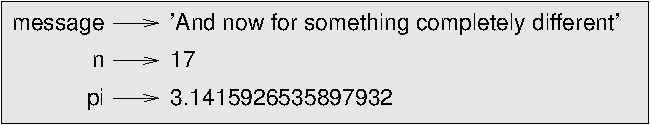
\includegraphics[scale=0.8]{figs/state2.pdf}}
\caption{State diagram.}
\label{fig.state2}
\end{figure}



\section{变量名}
\index{variable}

程序工程师一般会为变量选择容易理解的名称, 使人一看即知其用途. 

变量名可长可短, 可以包含字母和数字, 但不能以数字开头, 
大小写均可用, 但依惯例来说, 建议只用小写字母. 

变量名也可以使用\verb"_",  多用在形如\verb"your_name" 或 
\verb"airspeed_of_unladen_swallow" 这种多单词命名的变量名中. 
\index{underscore character}

如果变量名包含了非法字符, 就会报语法错误:

\begin{verbatim}
>>> 76trombones = 'big parade'
SyntaxError: invalid syntax
>>> more@ = 1000000
SyntaxError: invalid syntax
>>> class = 'Advanced Theoretical Zymurgy'
SyntaxError: invalid syntax
\end{verbatim}
%
变量名 {\tt 76trombones}不合法, 是因为以数字开头, 
而{\tt more@}不合法是因为包含了非法字符 {\tt @}. 
那么 {\tt class} 为什么也不正确呢?

这是因为 {\tt class}是Python的一个{\bf 关键字}. 
解释器用关键字(也称预留字)来识别代码结构, 所以它们不能用作变量名. 
\index{keyword}

Python 3包含以下关键字:

\begin{verbatim}
False      class      finally    is         return
None       continue   for        lambda     try
True       def        from       nonlocal   while
and        del        global     not        with
as         elif       if         or         yield
assert     else       import     pass
break      except     in         raise
\end{verbatim}
%

你无须记忆这些关键字. 在多数开发环境中, 关键字会以特殊颜色标识, 
所以如果将其误用作变量名时, 很容易发觉. 

\section{表达式和语句}

{\bf 表达式}是值, 变量以及运算符的组合. 
值本身可以认为是一个表达式, 同样, 变量也可以认为是一个表达式. 
所以下面都是合法的表达式:
\index{expression}

\begin{verbatim}
>>> 42
42
>>> n
17
>>> n + 25
42
\end{verbatim}
%
当根据提示符输入表达式时, 解释器会进行{\bf 估算}, 也就是说它会找到表达式的值. 
上例中, {\tt n} 的值是17, {\tt n+25} 的值是42. 
\index{evaluate}

 {\bf 语句} 是代码的基本有效单位, 例如新建变量或者显示值. 
\index{statement}

\begin{verbatim}
>>> n = 17
>>> print(n)
\end{verbatim}
%
第一行是为{\tt n}赋值的赋值语句, 第二行是显示{\tt n}结果的打印语句. 

当你键入语句, 解释器根据语句{\bf 执行}, 但通常, 语句是没有值的. 
\index{execute}


\section{脚本模式}

截至当前, 我们一直在{\bf 交互模式}下运行代码, 
这表示你可以直接与解释器进行交互.
入门学习采用交互模式尚可行, 
但代码行数一旦增多, 使用就会很麻烦. 
\index{interactive mode}

另一个替代方案是将代码保存至{\bf 脚本}文件, 然后在{\bf 脚本模式}
下运行解释器执行脚本. 按照惯例, Python脚本以 {\tt .py} 结尾. 
\index{script}
\index{script mode}

了解了如何创建以及运行脚本, 便可开启后续学习. 
如果没有配套工具, 建议继续采用PythonAnywhere. 
同时, 我已在\url{http://tinyurl.com/thinkpython2e}
撰写了脚本模式下执行代码的相关步骤. 

因为Python提供了这两种模式,  
所以你可以采用交互模式进行部分语句的验证,
然后将其发布到脚本中. 
但是两种模式多有差异, 可能会令人无所适从. 
\index{interactive mode}
\index{script mode}

例如, 以Python进行运算, 可以键入:

\begin{verbatim}
>>> miles = 26.2
>>> miles * 1.61
42.182
\end{verbatim}

首行代码给{\tt miles}赋值, 但是不显示任何结果. 
第二行是表达式, 解释器会对其求值, 并显示结果, 
事实证明, 马拉松大约为42公里. 

但是将相同代码写入脚本并运行, 不会有任何输出结果. 
表达式在脚本模式不会有任何可见效果, 如果需要显示结果, 
可以采用 {\tt print}语句: 

\begin{verbatim}
miles = 26.2
print(miles * 1.61)
\end{verbatim}

初次使用, 会感到奇怪. 为了验证你的理解, 
可以在Python解释器键入以下内容, 看看现象:

\begin{verbatim}
5
x = 5
x + 1
\end{verbatim}

将同样语句放入脚本并运行, 会如何?
如果将每个表达式都放入print语句中, 并运行, 又会如何?


\section{运算次序}
\index{order of operations}
\index{PEMDAS}

当表达式含有多个运算符时, 执行顺序主要基于 {\bf 运算次序}. 
对于数学运算符, Python 遵循数学惯例. 
采用缩写{\bf PEMDAS}可以辅助记忆这些规则:

\begin{itemize}

\item 括号({\bf P}arentheses)优先级最高, 可以据此按需调整运算次序. 
因为括号中的表达式会优先处理, 所以{\tt 2 * (3-1)}结果为 4, {\tt (1+1)**(5-2)}则为 8. 
又如{\tt (minute * 100) / 60}, 
虽然没有改变结果, 但使用括号令表达式更加易于阅读了. 

\item 幂运算({\bf E}xponentiation)优先级次之. 所以
{\tt 1 + 2**3} 是 9 而非 27,  且{\tt 2 * 3**2} 等于18 而非 36. 

\item 乘法({\bf M}ultiplication)和除法({\bf D}ivision)优先级高于加法({\bf A}ddition)
和减法({\bf S}ubtraction). 所以 {\tt 2*3-1} 等于5而非4, {\tt 6+4/2}等于8而非5. 

\item 对于同优先级的运算符, 遵照自左向右的顺序(除幂运算). 
 在表达式{\tt degrees / 2 * pi}中, 除法先执行, 结果再乘以{\tt pi}. 
如果想除以$2 \pi$,  可以使用括号处理或者改写为{\tt degrees / 2 / pi}. 

\end{itemize}

不必强求记忆这些运算符的优先级, 碰到比较复杂的表达式, 采用括号会方便很多. 


\section{字符串操作}
\index{string!operation}
\index{operator!string}

通常, 字符串不能使用数学运算符, 即使是类似数字的字符串也不能, 
因此下面的表达式均是非法运算:

\begin{verbatim}
'chinese'-'food'    'eggs'/'easy'    'third'*'a charm'
\end{verbatim}
%

但是有两个例外,  {\tt +} 和 {\tt *}. 

 {\tt +}可以实现{\bf 字符串拼接}, 也就是首尾相接. 例如:
\index{concatenation}

\begin{verbatim}
>>> first = 'throat'
>>> second = 'warbler'
>>> first + second
throatwarbler
\end{verbatim}
%
 {\tt *} 同样适用于字符串, 表示堆叠. 例如\verb"'Spam'*3" 表示
\verb"'SpamSpamSpam'". 如果其中一个值是字符串, 另外一个值就必须是整数. 

这种使用{\tt +} 和 {\tt *}的方式与加法和乘法类似. 
 {\tt 4*3} 等价于 {\tt 4+4+4}, 
而对于 \verb"'Spam'*3",  
我们也希望等价于 \verb"'Spam'+'Spam'+'Spam'", 也确实如此. 
但是, 字符串的拼接和堆叠与数字的加法和乘法, 有一个明显的不同之处. 
你是否可以想到, 加法具有, 而字符串拼接却没有的属性?

\index{commutativity}


\section{注释}
\index{comment}

随着代码量越来越庞大, 越来越复杂, 
阅读并理解其逻辑也越来越困难. 
编程语言使用时又写得密密麻麻, 
想通过一段代码去明白其逻辑和功能, 无异于海底捞针. 

所以, 在程序代码中加入一些自然语言备注说明, 
以解释其作用, 便显得异常重要. 
这些备注说明, 便叫做{\bf 注释},  一般以井号( \verb"#")开头:

\begin{verbatim}
# 计算所占一小时的百分比
percentage = (minute * 100) / 60
\end{verbatim}
%
此例中, 注释独占一行. 你也可以把注释放在代码末尾:

\begin{verbatim}
percentage = (minute * 100) / 60     # 所占一小时的百分比
\end{verbatim}
%
代码中所有{\tt \#}开头的行, 在执行过程中都会被忽略. 

在编码中实现特殊逻辑时, 注释尤为重要. 
但要注意, 说明编码的 {\em 缘由},
远胜于讲述代码的{\em 作用}. 

下面这条注释便显得多余:

\begin{verbatim}
v = 5     # 将 5 赋值给 v
\end{verbatim}
%

而下面的注释则包含了未体现在代码中的有用信息:

\begin{verbatim}
v = 5     # 速度(米/秒) 
\end{verbatim}
%
良好的变量命名可以减少注释的使用, 
但是过长的变量名, 又使得代码繁杂而难以阅读, 
所以如何取舍, 需要权衡. 


\section{调试}
\index{debugging}
\index{bug}

一般程序中会出现三种异常:
语法错误, 运行时错误以及语义错误. 
有效区分三者差异, 可以大大提高定位速度. 

\begin{description}

\item[语法错误:] ``语法''指的是程序结构以及使用规范. 
例如, 括号必须成对出现, 
所以{\tt (1 + 2)}正确, 而{\tt 8)}则是语法错误. 
\index{syntax error} 
\index{error!syntax}
\index{error message}
\index{syntax} 

如果程序存在语法错误, Python会直接报错并退出, 
程序便无法继续运行. 
开始学习编程时, 你可能需要耗费大量精力跟踪语法错误. 
但随着经验的积累, 你犯此类错误将会越来越少, 而定位也会越来越快.


\item[运行时错误:] 第二类错误是运行时错误, 
因为这种错误只有在程序开始运行后才会出现. 
这些错误也叫作{\bf 异常}, 
因为它们通常表示发生了异常(且不好的)情况. 
\index{runtime error} \index{error!runtime}
  \index{exception} \index{safe language} \index{language!safe}

本书前几章的程序较为简单, 运行时错误也较少遇到, 
所以想窥其全貌, 还需一段时间. 

\item[语义错误:] 第三种错误是 ``语义错误'', 
意如其字, 表示含义相关. 
如果程序中存在语义错误, 它不会报错, 只是不会按照预期的方式执行. 
具体来说, 便是会按照你的指示去做, 而不是你想要的去做.
\index{semantic error}
  \index{error!semantic} \index{error message}

识别语义错误可能很棘手, 需要你逆向处理, 
从输出查看, 回溯代码, 才能确定其逻辑. 

\end{description}


\section{术语表}

\begin{description}

\item[变量(variable):]  用来引用一个值的名称. 
\index{variable}

\item[赋值(assignment):] 为变量赋值的语句. 
\index{assignment}

\item[状态图(state diagram):] 一种图像化表示变量及所引用值的方式. 
\index{state diagram}

\item[关键字(keyword):] 编程语言用来解析代码的预留字, 像 {\tt if}、{\tt  def} 和 {\tt while}, 
均不能作为变量名使用. 
\index{keyword}

\item[操作数(operand):] 运算符操作的单一值对象. 
\index{operand}

\item[表达式(expression):] 变量、运算符以及值的组合, 
共同作用来表示单一结果. 
\index{expression}

\item[求值(evaluate):] 通过执行运算来简化表达式, 从而得到值的过程. 
\index{evaluate}

\item[语句(statement):] 表示命令或者操作的代码块. 目前遇到的语句是赋值语句以及打印语句. 
\index{statement}

\item[执行(execute):] 运行语句, 执行其指令.
\index{execute}

\item[交互模式(interactive mode):] 通过在提示符下输入代码
来使用Python解释器的一种方式. 
\index{interactive mode}

\item[脚本模式(script mode):] 通过从脚本中读取代码并执行, 
以使用Python解释器的一种方式. 
\index{script mode}

\item[脚本(script):] 存储代码的文件. 
\index{script}

\item[运算次序(order of operations):]  包含多运算符和操作数的表达式执行时所遵循的先后顺序. 
\index{order of operations}

\item[拼接(concatenate):] 操作数首位相接. 
\index{concatenation}

\item[注释(comment):] 帮助他人理解代码的有效信息, 对程序执行无影响. 
\index{comment}

\item[语法错误(syntax error):] 导致代码无法解析(因此无法解释)的错误. 
\index{syntax error}

\item[异常(exception):] 程序运行时遇到的错误. 
\index{exception}

\item[语义(semantics):] 代码含义. 
\index{semantics}

\item[语义错误(semantic error):] 未获得预期结果的错误. 
\index{semantic error}

\end{description}


\section{习题集}

\begin{exercise}

重申从上节便给出的建议, 学习新知识, 
尽量在交互模式下不断试错, 大胆假设, 小心求证. 

\begin{itemize}

\item 既然{\tt n = 42}正确, 那么{\tt 42 = n}呢?

\item {\tt x = y = 1}正确与否?

\item 在一些编程语言中, 每个语句都会以分号{\tt ;}结尾, 
如果在Python的语句末尾加上分号会怎样?

\item 语句末尾加句号会如何?

\item 数学公式中, 可以用 $x y$ 表示 $x$ 和 $y$ 相乘. Python中若如此使用会如何?

\end{itemize}

\end{exercise}


\begin{exercise}

使用Pyhton解释器作为计算器进行练习:
\index{calculator}

\begin{enumerate}

\item 半径$r$的球体体积是 $\frac{4}{3} \pi r^3$. 那半径为5的球体体积是多少?

\item 假设书原价\$24.95, 但书店拥有 40\% 的折扣. 
同时邮寄首件需要邮费\$3, 后续每件75美分, 
如果批发60件, 总费用多少?

\item 如果我早上6:52离家, 以慢跑方式 (8分15秒/每英里)跑了1英里, 然后以
快跑方式(7分12秒/每英里)跑了3英里, 最后, 又以慢跑方式跑了1英里, 
那我什么时候到家吃早餐?
\index{running pace}

\end{enumerate}
\end{exercise}


\chapter{函数}
\label{funcchap}

在编程领域, {\bf 函数}是指执行既定运算的语句组合. 
定义函数便是确定名称以及语句组合. 然后, 便可以通过函数名来``调用''函数. 
\index{function}

\section{函数调用}
\label{functionchap}
\index{function call}

上文已见过{\bf 函数调用}的例子:

\begin{verbatim}
>>> type(42)
<class 'int'>
\end{verbatim}
%
此函数的名称为{\tt type},  括号中的表达式叫做函数的{\bf 参数}. 
此处获得的结果, 是参数的类型. 
\index{parentheses!argument in}

通俗来说, 函数会``接受''参数, 并``返回''相应的结果. 
这个结果也叫做{\bf 返回值}. 
\index{argument}
\index{return value}

Python提供了值类型转换的函数, 正常情况下, 
{\tt int}函数可以将任意值转为整数, 
除非输入有误:
\index{conversion!type}
\index{type conversion}
\index{int function}
\index{function!int}

\begin{verbatim}
>>> int('32')
32
>>> int('Hello')
ValueError: invalid literal for int(): Hello
\end{verbatim}
%
{\tt int}函数虽然可以将浮点数转为整数, 
但不会四舍五入, 而是直接截取整数部分:

\begin{verbatim}
>>> int(3.99999)
3
>>> int(-2.3)
-2
\end{verbatim}
%
{\tt float}函数可以将整数及字符串格式小数转为浮点数:
\index{float function}
\index{function!float}

\begin{verbatim}
>>> float(32)
32.0
>>> float('3.14159')
3.14159
\end{verbatim}
%
最后, {\tt str} 函数可以将其参数转为字符串:
\index{str function}
\index{function!str}

\begin{verbatim}
>>> str(32)
'32'
>>> str(3.14159)
'3.14159'
\end{verbatim}
%

\section{数学函数}
\index{math function}
\index{function!math}

Pyhton内置了名为{\tt math}的模块, 提供了大量数学计算函数. 
{\bf 模块}是指包含一类相关函数的文件. 
\index{module}
\index{module object}

在使用模块中的函数前, 我们需要用{\bf import 语句}来导入模块:

\begin{verbatim}
>>> import math
\end{verbatim}
%
这个语句会创建一个名为{\tt math}的{\bf 模块对象}. 
输入模块对象名称, 可以看到一些相关信息:

\begin{verbatim}
>>> math
<module 'math' (built-in)>
\end{verbatim}
%
模块对象包含了模块中定义的函数和变量. 
若要调用相应函数, 需要指定模块名称和函数名称, 
中间用点(也可以当作英文中的句号)来分隔. 这种调用方法, 就是{\bf 点标法}. 
\index{dot notation}

\begin{verbatim}
>>> ratio = signal_power / noise_power
>>> decibels = 10 * math.log10(ratio)

>>> radians = 0.7
>>> height = math.sin(radians)
\end{verbatim}
%
第一个例子使用 \verb"math.log10" 计算分贝信噪比(已知 \verb"signal_power" 和
\verb"noise_power"). 
{\tt math}模块还提供了{\tt log}函数, 用于计算以{\tt e}为底的对数. 
\index{log function}
\index{function!log}
\index{sine function}
\index{radian}
\index{trigonometric function}
\index{function!trigonometric}

第二个例子是计算{\tt 弧度(radians)}的正弦值. 
{\tt 弧度} 一般作为三角函数({\tt sin}, {\tt cos}和 {\tt tan}, 等)的输入参数. 
而角度转弧度, 需要除以180然后乘以$\pi$:

\begin{verbatim}
>>> degrees = 45
>>> radians = degrees / 180.0 * math.pi
>>> math.sin(radians)
0.707106781187
\end{verbatim}
%
{\tt math.pi} 表达式是从math模块获取变量{\tt pi}, 
这是一个 $\pi$的浮点格式近似值, 
精确到小数点后约15位. 
\index{pi}

如果熟悉三角函数原理, 
便可以通过与 $\frac{ \sqrt{2}} {2}$ 比较来验证结果:
\index{sqrt function}
\index{function!sqrt}

\begin{verbatim}
>>> math.sqrt(2) / 2.0
0.707106781187
\end{verbatim}
%

\section{组合}
\index{composition}

到目前为止, 我们学习了编程涉及的各个元素---变量, 表达式以及语句. 
但都是分开来讲, 并未整合在一起. 

编程语言的强大之处在于, 可以构建众多的小积木, 然后 {\bf 组合}起来. 
例如, 函数的参数既然可以是各种表达式, 那自然包括算数运算:

\begin{verbatim}
x = math.sin(degrees / 360.0 * 2 * math.pi)
\end{verbatim}
%
也可以是函数调用:

\begin{verbatim}
x = math.exp(math.log(x+1))
\end{verbatim}
%
任何可以使用值的地方, 都可以使用表达式来替换, 除了一种情况:
赋值语句的左侧必须是变量名. 
左侧出现任何表达式都会报语法错误(但稍后会看到此规则的例外情况). 

\begin{verbatim}
>>> minutes = hours * 60                 # right
>>> hours * 60 = minutes                 # wrong!
SyntaxError: can't assign to operator
\end{verbatim}
%
\index{SyntaxError}
\index{exception!SyntaxError}


\section{创建函数}

到目前, 我们在Python编程中多使用的是内置函数, 但现在可以尝试创建一个函数. 
{\bf 函数定义} 一般是指定义函数名称以及调用函数时所运行的一系列语句组合. 
\index{function}
\index{function definition}
\index{definition!function}

这是一个示例:

\begin{verbatim}
def print_lyrics():
    print("I'm a lumberjack, and I'm okay.")
    print("I sleep all night and I work all day.")
\end{verbatim}
%

{\tt def}关键字表示这是一个函数定义. 
函数名是 \verb"print_lyrics". 
函数名的命名规则和变量名命名规则一致: 
可包含字母, 数字或下划线, 但第一个字符不能为数字. 
同时不能使用关键字作为函数名, 要避免变量和函数重名. 
\index{def keyword}
\index{keyword!def}
\index{argument}

函数名后的空括号表示这个函数不带任何参数. 
\index{parentheses!empty}
\index{header}
\index{body}
\index{indentation}
\index{colon}

函数定义首行一般叫做 {\bf 函数头}, 其余部分叫{\bf 函数体}.
函数头以冒号结尾, 函数体必须缩进. 
依照惯例, 一个缩进等于四个空格. 
函数体可以包含任意行语句. 

print语句中的字符串需要被双引号包着. 
一般单引号和双引号作用相同, 所以人们多数情况使用单引号, 
除非字符串中本来就有单引号, 这种情况就要使用双引号了. 

所有的引号(无论单双)都是 ``直引号'', 通常位于键盘确认键(Enter)旁边, 
像本句中这种``弯引号'', 在Python使用中是不合法的. 

在交互模式下定义函数, 解释器会打省略号({\tt ...}) 以表示函数定义尚不完整:
\index{ellipses}

\begin{verbatim}
>>> def print_lyrics():
...     print("I'm a lumberjack, and I'm okay.")
...     print("I sleep all night and I work all day.")
...
\end{verbatim}
%
要结束函数定义, 需要多敲一个换行. 

函数定义完成便会创建一个 \verb"function" 类型的 {\bf 函数对象}:
\index{function type}
\index{type!function}

\begin{verbatim}
>>> print(print_lyrics)
<function print_lyrics at 0xb7e99e9c>
>>> type(print_lyrics)
<class 'function'>
\end{verbatim}
%
调用自定义函数和调用内置函数的方式一样:

\begin{verbatim}
>>> print_lyrics()
I'm a lumberjack, and I'm okay.
I sleep all night and I work all day.
\end{verbatim}
%
一旦定义了一个函数, 便可在其他函数中使用它. 
例如, 为了重复之前的歌词, 
我们可以编写一个名为\verb"repeat_lyrics" 的函数:

\begin{verbatim}
def repeat_lyrics():
    print_lyrics()
    print_lyrics()
\end{verbatim}
%
然后调用\verb"repeat_lyrics":

\begin{verbatim}
>>> repeat_lyrics()
I'm a lumberjack, and I'm okay.
I sleep all night and I work all day.
I'm a lumberjack, and I'm okay.
I sleep all night and I work all day.
\end{verbatim}
%
但这并不是歌曲的真正歌词. 

\section{定义和调用}
\index{function definition}

将上一节的代码片段组合在一切, 看起来便是这样:

\begin{verbatim}
def print_lyrics():
    print("I'm a lumberjack, and I'm okay.")
    print("I sleep all night and I work all day.")

def repeat_lyrics():
    print_lyrics()
    print_lyrics()

repeat_lyrics()
\end{verbatim}
%
此程序包含两个函数定义: \verb"print_lyrics" 和 \verb"repeat_lyrics". 
这些函数定义的执行和其他语句一样, 但是会在执行后创建函数对象. 
函数内的语句只有在函数被调用时才会执行, 同时函数定义本身并不会输出结果. 
\index{use before def}

如你所料, 函数运行前需要先创建函数, 也就是说, 
函数定义必须在函数调用之前执行. 

做个练习, 将程序的末行提到开始, 令函数先被调用, 再被定义. 
运行程序, 看看会报什么错误. 

将函数调用再次移回末尾, 然后将 \verb"print_lyrics" 的函数定义
放到 \verb"repeat_lyrics" 的定义之后, 运行程序, 会发生什么?

\section{执行流程}
\index{flow of execution}

为保证函数定义先于函数调用, 你需要了解语句执行顺序, 
这被称为{\bf 执行流程}. 

程序代码从第一行开始, 从上到下, 逐行运行. 

执行函数定义不会改变程序执行流程, 
但是要谨记, 函数内的语句只会在函数被调用时才执行. 

函数调用就像执行流程中的绕路, 不会继续向下执行语句, 
而是跳转到函数体内, 执行其中语句, 完成后再回到离开的地方, 
继续执行之前的语句. 

听起来很简单, 但是要意识到, 函数可以不断调用函数({\tt 译者注: 类似套娃}).
甲函数运行中, 可能会调用乙函数, 从而去执行其语句, 
然后乙函数运行中又可能去调用其他函数!

幸亏Python解释器能够有效追踪函数的执行流程, 才可以在函数执行完成后, 
回到函数被调用的地方, 继续执行, 直到结束. 

总之, 当你阅读程序时, 不要总是自上而下阅读程序, 
有时候按照执行流程来阅读更便于理解. 


\section{形参和实参}
\label{parameters}
\index{parameter}
\index{function parameter}
\index{argument}
\index{function argument}

我们观察到有些函数需要参数. 例如调用{\tt math.sin}函数, 需要传递数值作为参数. 
还有些函数不止一个参数:{\tt math.pow} 需要两个参数, 分别是底和幂. 

函数内, 实参会被赋值给{\bf 形参}. 
下面是函数传参(实参赋值给形参)的例子:
\index{parentheses!parameters in}

\begin{verbatim}
def print_twice(bruce):
    print(bruce)
    print(bruce)
\end{verbatim}
%
此函数会将实参赋值给形参{\tt bruce}, 当此函数被调用时, 
会输出两次参数值(无论参数为何). 

此函数适用于任何可被打印的值. 

\begin{verbatim}
>>> print_twice('Spam')
Spam
Spam
>>> print_twice(42)
42
42
>>> print_twice(math.pi)
3.14159265359
3.14159265359
\end{verbatim}
%
自定义函数和内置函数的适用规则是一致的, 
所以\verb"print_twice"的实参也可以是任意表达式:
\index{composition}
\index{programmer-defined function}
\index{function!programmer defined}

\begin{verbatim}
>>> print_twice('Spam '*4)
Spam Spam Spam Spam
Spam Spam Spam Spam
>>> print_twice(math.cos(math.pi))
-1.0
-1.0
\end{verbatim}
%
实参会在函数调用前被计算, 所以在上例中, 表达式 \verb"'Spam '*4" 和
{\tt math.cos(math.pi)}只会被计算一次. 
\index{argument}

你也可以使用变量作为实参:

\begin{verbatim}
>>> michael = 'Eric, the half a bee.'
>>> print_twice(michael)
Eric, the half a bee.
Eric, the half a bee.
\end{verbatim}
%
函数实参的变量命名({\tt michael})和函数形参的命名({\tt bruce})没有关系. 
无论外部传递进来的值如何命名, 函数 \verb"print_twice"内部, 我们统称其为 {\tt bruce}. 


\section{局部变量和参数}
\index{local variable}
\index{variable!local}

函数内部定义的变量都是{\bf 局部}的, 也就是说, 只能作用于函数内部, 
例如:
\index{parentheses!parameters in}

\begin{verbatim}
def cat_twice(part1, part2):
    cat = part1 + part2
    print_twice(cat)
\end{verbatim}
%
此函数将两个参数拼接后, 结果输出两次. 以下是用例:
\index{concatenation}

\begin{verbatim}
>>> line1 = 'Bing tiddle '
>>> line2 = 'tiddle bang.'
>>> cat_twice(line1, line2)
Bing tiddle tiddle bang.
Bing tiddle tiddle bang.
\end{verbatim}
%
\verb"cat_twice"运行结束, 内部变量{\tt cat}便被销毁. 
如果现在尝试打印它, 会报错:
\index{NameError}
\index{exception!NameError}

\begin{verbatim}
>>> print(cat)
NameError: name 'cat' is not defined
\end{verbatim}
%
形参都是局部的, 例如变量{\tt bruce}便不会出现在\verb"print_twice" 函数之外.
\index{parameter}


\section{栈图}
\label{stackdiagram}
\index{stack diagram}
\index{function frame}
\index{frame}
若想跟踪变量使用情况, 一般绘制{\bf 栈图}比较有效. 
和状态图类似, 栈图也会标识每个变量的值, 不同之处是, 
栈图会标识变量所属函数. 
\index{stack diagram}
\index{diagram!stack}

每个函数都用一个{\bf 框} 来表示, 一个框就是一个旁边有函数名, 
内部是参数以及变量值的箱体图. 
前述例子的栈图见图~\ref{fig.stack}. 

\begin{figure}
\centerline
{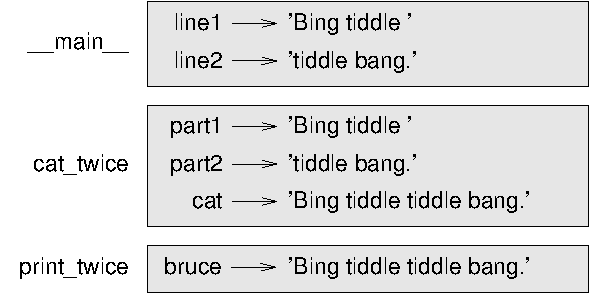
\includegraphics[scale=0.8]{figs/stack.pdf}}
\caption{栈图.}
\label{fig.stack}
\end{figure}

栈图中的各个框的排列方式标示了各个函数的调用关系. 
此例中, \verb"print_twice"函数被 \verb"cat_twice"调用, 
\verb"cat_twice" 被\verb"__main__"调用. \verb"__main__"是
顶层框的一个特殊名称, 任何函数外的变量, 都属于它. 
\index{main}

形参和实参是一一对应的, 所以{\tt part1} 和{\tt line1}的值相同, 
{\tt part2} 和{\tt line2}的值也相同, 并且, 
 {\tt bruce} 和{\tt cat}的值也一样. 

如果函数在调用过程中出错, Python会打印出函数名称, 
以及调用它的上级函数信息, 以及更上级的函数, 一直到 \verb"__main__" 函数.

例如, 如果在\verb"print_twice" 中调用{\tt cat}, 会得到名称错误({\tt NameError}):

\begin{verbatim}
Traceback (innermost last):
  File "test.py", line 13, in __main__
    cat_twice(line1, line2)
  File "test.py", line 5, in cat_twice
    print_twice(cat)
  File "test.py", line 9, in print_twice
    print(cat)
NameError: name 'cat' is not defined
\end{verbatim}
%
这一系列跟踪函数的信息叫做{\bf 溯源}, 这些信息会显示是哪个文件出错, 哪行出错, 
以及运行时函数, 甚至引起错误的代码行号. 
\index{traceback}

在溯源信息中的函数次序和栈图中的框的次序是一致的, 
当前正在运行的函数都是在最下面. 

\section{有值函数和无值函数}
\index{fruitful function}
\index{void function}
\index{function!fruitful}
\index{function!void} 

目前用到过的一些函数, 例如math函数, 都会返回结果, 
一得之见, 暂称{\bf 有值函数}. 其他函数, 像 \verb"print_twice", 
运行完成, 并不会返回值, 便叫做{\bf 无值函数}. 

当调用有值函数时, 一般是希望对返回结果另行处理, 比如, 
将结果赋值给某个变量, 或者作为表达式一部分使用:

\begin{verbatim}
x = math.cos(radians)
golden = (math.sqrt(5) + 1) / 2
\end{verbatim}
%
在交互模式调用函数, Python解释器总会输出结果:

\begin{verbatim}
>>> math.sqrt(5)
2.2360679774997898
\end{verbatim}
%
但是在脚本模式, 调用有值函数, 却永远不会看到返回值!

\begin{verbatim}
math.sqrt(5)
\end{verbatim}
%
这个脚本计算5的平方根, 但因为没有保存或者显示结果, 所以不是很有用. 
\index{interactive mode}
\index{script mode}

无值函数可以在屏幕显示信息或者制造其他效果, 
只是不会有返回值. 如果将函数运行结果赋值到某个变量, 
那变量会指向一个特殊的值:{\tt None}.
\index{None special value}
\index{special value!None}

\begin{verbatim}
>>> result = print_twice('Bing')
Bing
Bing
>>> print(result)
None
\end{verbatim}
%
{\tt None}是个具有既定类型的特殊值, 和字符串 \verb"'None'"是不同的:

\begin{verbatim}
>>> type(None)
<class 'NoneType'>
\end{verbatim}
%
截至目前, 我们定义的函数都是无返回值的, 
后续章节将开始定义有返回值的函数. 
\index{NoneType type}
\index{type!NoneType}


\section{函数何用}
\index{function!reasons for}

将程序划分为一个个函数是否值得, 对此的考量, 可以参看以下缘由:

\begin{itemize}

\item 函数可以将一组语句起个名字, 使程序便于阅读和调试. 

\item 函数可以消除重复, 简化代码, 针对功能, 修改一处即可. 

\item 将程序切分为函数, 可以分别调试, 然后组合它们即可. 

\item 设计良好的函数对许多程序都有用, 一旦编写调试了一个函数, 
便可以多次复用. 

\end{itemize}


\section{调试}

编程最重要的技能之一就是调试了, 虽往往令人黯然神伤, 愁眉难舒, 
却是编程中最考验才智, 最富有挑战同时最有趣的地方.
\index{experimental debugging}
\index{debugging!experimental}

在某些方面, 调试和侦探工作很像. 面对线索, 有效推理, 确定造就结果的流程和缘由. 

调试也像实验科学, 针对问题, 一旦有所想法, 便可修改程序, 再次尝试. 
如果假设正确, 便可预期修改后的结果, 向可执行的程序代码推进. 
如果假设错误, 便要继续探究了. 正如Sherlock Holmes(夏洛克·福尔摩斯)所说, 
``当你排除所有不可能因素, 留下来的东西, 即使看似不可能, 也必定是
真相."(A. Conan Doyle, {\em The Sign of Four})
\index{Holmes, Sherlock}
\index{Doyle, Arthur Conan}

对某些人而言, 编程便是调试. 这是因为, 编程便是不断调试程序, 直到实现目标的过程. 
所以, 你应该从一个能够工作的程序开始, 逐步进行小的修改, 并在修改的同时进行调试. 

比如, Linux 操作系统具有数百万行代码,  但它最初只是一个Linus Torvalds
探索Intel 80386芯片的简单代码. 根据Larry Greenfield的说法, 
``Linus的早期项目中, 有个在打印AAAA和BBBB之间切换的程序, 而这后来演化为了Linux.''
({\em The Linux Users' Guide} Beta Version 1).
\index{Linux}


\section{术语表}

\begin{description}

\item[函数(function):] 特别命名的一组语句序列, 实现特定功能. 可以有参数, 
也可以没有参数, 可以返回值, 也可以不返回. 
\index{function}

\item[函数定义(function definition):] 创建函数的语句, 会指定名称, 参数以及内部语句. 
\index{function definition}

\item[函数对象(function object):] 函数定义创建的值, 函数名便是指向函数对象的变量. 
\index{function object}

\item[函数头(header):] 函数定义的首行.
\index{header}

\item[函数体(body):] 函数定义的内部语句序列.
\index{body}

\item[形参(parameter):] 函数内部用来引用传入值的名称. 
\index{parameter}

\item[函数调用(function call):] 运行函数的语句, 由函数名, 以及括号中的参数列表构成. 
\index{function call}

\item[实参(argument):] 函数调用时传入函数的值. 这个值会赋值给函数内部的形参. 
\index{argument}

\item[局部变量(local variable):] 函数内部定义的变量, 局部变量只能在其所属函数内部使用. 
\index{local variable}

\item[返回值(return value):] 函数返回的结果. 如果用函数调用作为表达式, 那么函数返回值, 便是表达式的值. 
\index{return value}

\item[有值返回(fruitful function):] 有返回值的函数. 
\index{fruitful function}

\item[无值返回(void function:] 返回值为{\tt None}的函数. 
\index{void function}

\item[空值({\tt None}):] 无值返回函数返回的结果. 
\index{None special value}
\index{special value!None}

\item[模块(module):] 包含相关函数以及定义的文件. 
\index{module}

\item[导入语句(import statement):] 读取模块文件并创建模块对象的语句. 
\index{import statement}
\index{statement!import}

\item[模块对象(module object):] {\tt import}语句创建的值, 通过其可以获取模块内部的值. 
\index{module object}

\item[点标法(dot notation):] 通过在模块名后紧跟一个点(英文句号)和要调用的函数名, 
来调用模块函数的语法. 
\index{dot notation}

\item[组合(composition):] 采用简单表达式构建复杂表达式, 简单语句塑造复杂模块的方法. 
\index{composition}

\item[执行流程(flow of execution):] 语句的执行顺序.
\index{flow of execution}

\item[栈图(stack diagram):] 表示函数,变量,以及值的关系图. 
\index{stack diagram}

\item[框(frame):] 栈图中表示函数调用的方框,包括局部变量以及参数. 
\index{function frame}
\index{frame}

\item[溯源(traceback):] 异常发生时, 打印的正在执行的函数列表. 
\index{traceback}


\end{description}


\section{习题集}

\begin{exercise}
\index{len function}
\index{function!len}

编写名为 \verb"right_justify" 同时以字符串{\tt s}为参数的函数, 
其输出的字符串左侧有足够的空格, 以使输出结果的最后一个字符在第70字符处. 

\begin{verbatim}
>>> right_justify('monty')
                                                                 monty
\end{verbatim}

提示: 使用字符串拼接以及堆叠操作. 此外, Python提供了内置函数{\tt len}, 可以返回字符串长度, 
因此\verb"len('monty')"的结果为5.

\end{exercise}


\begin{exercise}
\index{function object}
\index{object!function}

函数对象可以赋值给变量, 或者作为实参传递. 
例如, \verb"do_twice"便是一个接受函数对象作为参数, 并调用两次的函数:

\begin{verbatim}
def do_twice(f):
    f()
    f()
\end{verbatim}

下面是使用\verb"do_twice"来调用函数\verb"print_spam"两次的例子. 

\begin{verbatim}
def print_spam():
    print('spam')

do_twice(print_spam)
\end{verbatim}

\begin{enumerate}

\item 将上述代码写入脚本进行测试.

\item 修改 \verb"do_twice", 给其接受两个参数: 函数对象和值, 
使其调用两次传入的函数对象, 这个函数对象会以传入的值为参数.

\item 将先前章节中定义的\verb"print_twice"代码复制到脚本.

\item 用修改后的 \verb"do_twice"函数调用 \verb"print_twice"函数两次, 
同时传入参数 \verb"'spam'".

\item 定义新函数\verb"do_four", 令其接收函数对象和值, 
并以值为参数调用四次函数对象. 
要求函数体只有两条语句, 而不是四条. 

\end{enumerate}

答案: \url{http://thinkpython2.com/code/do_four.py}.

\end{exercise}



\begin{exercise}

说明: 此习题应该只使用我们学过的语句和特性来完成. 

\begin{enumerate}

\item 编写绘制下面网格图的函数:
\index{grid}

\begin{verbatim}
+ - - - - + - - - - +
|         |         |
|         |         |
|         |         |
|         |         |
+ - - - - + - - - - +
|         |         |
|         |         |
|         |         |
|         |         |
+ - - - - + - - - - +
\end{verbatim}
%
提示: 要在一行上打印多个值, 可以通过打印逗号分隔的值序列来实现:

\begin{verbatim}
print('+', '-')
\end{verbatim}
%
默认情况, {\tt print}会换到下一行, 但可以覆盖这种行为, 
使其以空格结尾, 如下:

\begin{verbatim}
print('+', end=' ')
print('-')
\end{verbatim}
%
上边语句会将\verb"'+ -'"在同一行输出, 下一个print语句的输出, 则会另起一行. 

\item 编写一个函数, 以四行四列的形式绘制类似网格. 

\end{enumerate}

答案: \url{http://thinkpython2.com/code/grid.py}.
致谢: 此习题基于Oualline的书
({\em Practical C Programming, Third Edition},  
O'Reilly Media, 1997)中的一个练习.

\end{exercise}


\chapter{案例分析: 接口设计}
\label{turtlechap}

本章采用案例来讲述, 如何设计可以协同运行的函数. 

主要介绍 {\tt turtle(乌龟)}模块, 可以让你用其绘图功能, 制作图片. 
大部分Python安装包会预装{\tt turtle}模块, 但如果你使用的是PythonAnywhere网站, 
现在还无法执行turtle示例(至少撰写本书时还不能). 

如果你的计算机安装了Python, 便可以直接运行这些实例. 
如果还没有, 那么最好现在安装吧, 可以参看我写的
操作步骤\url{http://tinyurl.com/thinkpython2e}. 

本章的代码样例可以从\url{http://thinkpython2.com/code/polygon.py}获取. 


\section{模块turtle}
\label{turtle}

打开Python解释器, 键入以下命令, 以检查是否安装{\tt turtle}模块:

\begin{verbatim}
>>> import turtle
>>> bob = turtle.Turtle()
\end{verbatim}

运行此代码, 会创建一个窗口, 此窗口包含一个箭头, 代表一只小乌龟. 
关闭窗口. 

创建名为{\tt mypolygon.py} 的文件, 并输入以下代码:

\begin{verbatim}
import turtle
bob = turtle.Turtle()
print(bob)
turtle.mainloop()
\end{verbatim}
%
{\tt turtle}模块(小写字母 't')提供了函数{\tt Turtle}(大写字母 'T'), 
可以用来创建Turtle 对象, 我们将其分配给名为{\tt bob}的变量. 
输出{\tt bob}会显示如下类似信息:

\begin{verbatim}
<turtle.Turtle object at 0xb7bfbf4c>
\end{verbatim}
%
这意味着{\tt bob}指向了一个类型为{\tt Turtle}的对象, 
该对象是在模块{\tt turtle}中定义的.

\verb"mainloop" 会令窗口等待, 以执行其他操作. 但是本例
只需关闭窗口, 暂不进行其他操作. 

一旦创建了Turtle对象, 便可以调用{\bf 方法}在窗口中移动它. 
方法和函数类似, 但是略有不同. 比如, 令小乌龟前进:

\begin{verbatim}
bob.fd(100)
\end{verbatim}
%
方法{\tt fd}来自于乌龟对象{\tt bob}. 
调用方法就好比递交申请: 请求{\tt bob}向前移动. 

{\tt fd} 的参数是像素距离, 实际距离取决于屏幕尺寸. 

其他可以调用的方法还有{\tt bk}, 实现向后移动, 
{\tt lt}实现左转, {\tt rt}实现右转. 
{\tt lt} 和 {\tt rt}的参数都是以度为单位的角度. 

同时, 每个乌龟都带着笔, 可以抬起或落下;
如果笔落下, 乌龟移动时会留下痕迹. 
{\tt pu}和{\tt pd}方法分别表示``抬笔(pen up)''和``落笔(pen down)''.

将下面代码加入程序, 以实现绘制直角(
在创建{\tt bob}对象后, 以及调用\verb"mainloop"之前):

\begin{verbatim}
bob.fd(100)
bob.lt(90)
bob.fd(100)
\end{verbatim}
%
运行程序, 可以看到{\tt bob}对象会向东移动, 然后向北移动, 并留下两个线段. 

现在修改程序, 尝试绘制个正方形, 在实现之前, 先不要着急学习下面的内容. 

%\newpage

\section{简单重复}
\label{repetition}
\index{repetition}

你可能会写成下面的样子:

\begin{verbatim}
bob.fd(100)
bob.lt(90)

bob.fd(100)
bob.lt(90)

bob.fd(100)
bob.lt(90)

bob.fd(100)
\end{verbatim}
%
我们可以用{\tt for}语句更简洁地完成同样的操作. 
将下面代码写入{\tt mypolygon.py}并再次运行:
\index{for loop}
\index{loop!for}
\index{statement!for}

\begin{verbatim}
for i in range(4):
    print('Hello!')
\end{verbatim}
%
所见如下:

\begin{verbatim}
Hello!
Hello!
Hello!
Hello!
\end{verbatim}
%
这是{\tt for}语句的简单使用, 后面会有更多示例. 
但这足以让你重写正方形的绘制程序. 
暂时不要看下面的内容, 先尝试一下. 

下面是一个绘制正方形的{\tt for}语句示例:

\begin{verbatim}
for i in range(4):
    bob.fd(100)
    bob.lt(90)
\end{verbatim}
%
{\tt for}语句的语法使用类似函数定义. 
以冒号结尾的语句为函数头, 
缩进的内容为函数体. 
函数体可以包含任意数量的语句. 

{\tt for}语句也叫{\bf 循环}, 因为代码执行流程会重复执行循环体, 
此例中, 会执行四次循环体.
\index{loop}

这一版代码和上一版略有不同, 绘制完最后一条边后, 会做额外的转向. 
虽然这额外的旋转需要更多的时间, 但是如果我们每次循环都做同样的事情, 
可以简化代码. 
当然, 这个版本也有将小乌龟留在起始位置, 并朝向起始方向的效果. 

\section{习题集}
以下为一系列操作{\tt turtle} 模块的练习. 
它们旨在让你玩得开心, 但也有一定的重点. 
做练习的时候, 要好好思考一下重点是什么. 

习题后面有答案, 因此在完成(或至少尝试)之前, 先不要查看. 

\begin{enumerate}

\item 编写{\tt square}函数, 参数是个turtle对象{\tt t}, 用turtle绘制正方形. 

编写一个函数调用, 将{\tt bob} 作为参数传给{\tt square}, 然后运行程序. 

\item 为{\tt square}添加参数{\tt length}, 修改函数体, 令边的长度为{\tt length}, 
同时修改函数, 令其调用第二个实参. 再次运行程序, 使用不同的值测试{\tt length}的范围. 

\item 复制{\tt square}并命名为 {\tt polygon}. 添加另一个参数{\tt n},
并修改函数, 令其绘制正n边形. 提示: 正n边形外角角度为$360/n$度. 
\index{polygon function} 
\index{function!polygon}

\item 编写{\tt circle} 函数, 以turtle类型的{\tt t}, 以及半径{\tt r}为参数, 
通过使用适当长度和边数, 来调用{\tt polygon}函数, 绘制一个近似的圆. 
用不同的 {\tt r}值, 测试程序. \index{circle function} \index{function!circle}

提示: 确定圆的周长, 使其满足{\tt 边长 * 边数 = 周长}.

\item 升级{\tt circle}版本, 命名为{\tt arc}, 新增参数 {\tt angle}, 
用此值确定所绘制的圆弧的大小. 
{\tt angle}以度为单位, 当{\tt angle=360}, {\tt arc}会绘制一个完整的圆. 
\index{arc function}
\index{function!arc}

\end{enumerate}


\section{封装}

第一道题是编写绘制正方形的函数代码, 然后传递turtle参数, 并调用函数. 
代码如下:

\begin{verbatim}
def square(t):
    for i in range(4):
        t.fd(100)
        t.lt(90)

square(bob)
\end{verbatim}
%
函数内的 {\tt fd} 和 {\tt lt}缩进两次, 表示运行于函数定义里面的{\tt for} 循环中. 
下一行 {\tt square(bob)}, 左边距对齐同时没有缩进, 
这表示{\tt for} 循环以及函数定义的结束. 

函数内的 {\tt t} 和 {\tt bob}指向的是同一个乌龟对象, 
因此{\tt t.lt(90)}就好比 {\tt bob.lt(90)}. 
那么为何不直接用变量 {\tt bob}呢?
这是因为{\tt t}可以代指任意乌龟对象, 而不仅仅是 {\tt bob}, 
因此也可以再创建一个乌龟对象, 并作为参数传入 {\tt square}:

\begin{verbatim}
alice = turtle.Turtle()
square(alice)
\end{verbatim}
%
将一段代码写在函数中, 叫做{\bf 封装}. 
封装的好处之一在于, 用一个简单的名字来指代一段代码, 类似文档说明. 
另一个好处是可以复用代码, 调用函数两次总比复制粘贴大段的代码要更简洁!
\index{encapsulation}


\section{泛化}

下一步是给{\tt square}增加参数 {\tt length} , 详见下例:

\begin{verbatim}
def square(t, length):
    for i in range(4):
        t.fd(length)
        t.lt(90)

square(bob, 100)
\end{verbatim}
%
给函数增加参数, 叫做{\bf 泛化}. 
因为可以令函数更通用:
上版代码中, 正方形的边长总是相同大小, 
而此版, 边长可以是任意大小.
\index{generalization}

下一步也是泛化. 令{\tt polygon}实现绘制任意多边形, 
而不是只绘制正方形, , 详见示例:

\begin{verbatim}
def polygon(t, n, length):
    angle = 360 / n
    for i in range(n):
        t.fd(length)
        t.lt(angle)

polygon(bob, 7, 70)
\end{verbatim}
%
上面代码绘制了边长为70的正七边形. 

如果你使用的是Python 2, {\tt angle} 的值可能因为整除而出现偏差. 
有个简单的办法, 便是{\tt angle = 360.0 / n}. 分子为浮点数, 结果便也是浮点数了. 
\index{Python 2}

当函数有多个数值参数时, 很容易混淆各自代表什么, 或者参数顺序. 
这种情况下, 通常最好在传递实参列表时, 附上形参的名字:

\begin{verbatim}
polygon(bob, n=7, length=70)
\end{verbatim}
%
这也叫做{\bf 关键字参数}, 因为是把形参的名字作为 ``关键字''包含进来. 
(不要同Python中 {\tt while}和{\tt def}这种内置关键字混淆). 
\index{keyword argument}
\index{argument!keyword}

这种语法令程序可读性更强. 同时也提示了实参和形参的工作原理:
调用函数时, 实参赋值给了形参. 


\section{接口设计}

下一步要编写{\tt circle}, 此函数以半径{\tt r}为参数. 
以下是采用{\tt polygon}来绘制正五十边形的简单解决方案:

\begin{verbatim}
import math

def circle(t, r):
    circumference = 2 * math.pi * r
    n = 50
    length = circumference / n
    polygon(t, n, length)
\end{verbatim}
%
首行根据公式 $2 \pi r$和半径{\tt r} 计算圆的周长. 
要使用{\tt math.pi},  需要先导入{\tt math}. 
通常{\tt import}语句位于脚本开头. 

{\tt n}是要逼近圆的正多边形的边数, {\tt length} 表示边长. 
最后,  {\tt polygon}通过绘制正五十边形, 来逼近半径 {\tt r}的圆. 

此方案的局限性在于, {\tt n} 是一个常量, 这表示绘制非常大的圆时, 线段过长. 
而绘制小圆时, 需要耗费时间绘制小线段. 
要想使此函数通用, 可以将{\tt n}作为参数传入通用化的函数. 
这将为用户( {\tt circle}的调用者)提供更多控制权, 但是接口会显得不那么简洁了. 
\index{interface}

函数{\bf 接口} 是函数用途的摘要: 参数是什么? 函数做什么? 返回什么? 
如果一个接口允许调用者执行所需操作, 而无需处理无关的细节, 那么这个接口就是``简洁''的. 

在此示例中, {\tt r}放在接口中合适, 是因为要用它来确定圆的大小. 
而{\tt n}放进接口则显得不太友好, 是因为它只与{\em 如何}绘制圆的细节有关. 

与其令接口复杂, 不如根据{\tt 周长}来确定一个合适的{\tt n}:

\begin{verbatim}
def circle(t, r):
    circumference = 2 * math.pi * r
    n = int(circumference / 3) + 3
    length = circumference / n
    polygon(t, n, length)
\end{verbatim}
%
现在边的个数便是近似 {\tt circumference/3}的整数, 
每个边的长度也就近似于3了, 用这个长度, 绘制大圆快速, 小圆好看, 
对任意尺寸的圆都适用. 

给{\tt n}加3是为了保证多边形至少有3条边. 

\section{重构}
\label{refactoring}
\index{refactoring}

我们可以复用{\tt polygon}来构造{\tt circle}, 是因为边足够多的正多边形近似于圆. 
但是, 构造 {\tt arc}就不适合了, 因为没有办法用 {\tt polygon}或者{\tt circle}来绘制一段弧线. 

一个替代策略是复制{\tt polygon}, 将其修改为{\tt arc}, 代码如下:

\begin{verbatim}
def arc(t, r, angle):
    arc_length = 2 * math.pi * r * angle / 360
    n = int(arc_length / 3) + 1
    step_length = arc_length / n
    step_angle = angle / n
    
    for i in range(n):
        t.fd(step_length)
        t.lt(step_angle)
\end{verbatim}
%
函数后半段和 {\tt polygon}很像, 但如果我们不调整接口, 便无法复用 {\tt polygon}. 
我们需要给 {\tt polygon} 加入角度作为第三个参数, 来泛化它, 
那么也不能继续使用 {\tt polygon}作为名字了!
反而叫{\tt polyline}会更合适些:

\begin{verbatim}
def polyline(t, n, length, angle):
    for i in range(n):
        t.fd(length)
        t.lt(angle)
\end{verbatim}
%
现在我们需要重写{\tt polygon}和{\tt arc}, 以使用{\tt polyline}:

\begin{verbatim}
def polygon(t, n, length):
    angle = 360.0 / n
    polyline(t, n, length, angle)

def arc(t, r, angle):
    arc_length = 2 * math.pi * r * angle / 360
    n = int(arc_length / 3) + 1
    step_length = arc_length / n
    step_angle = float(angle) / n
    polyline(t, n, step_length, step_angle)
\end{verbatim}
%
最后, 我们重写{\tt circle}, 以使用{\tt arc}:

\begin{verbatim}
def circle(t, r):
    arc(t, r, 360)
\end{verbatim}
%
此过程---调整代码, 优化接口, 便于复用---叫做{\bf 重构}. 
此案例中, 我们发现{\tt arc}和{\tt polygon}具有一些相似代码, 
所以将其``抽离''为{\tt polyline}.\
\index{refactoring}

如果早有规划, 我们可能会优先编写{\tt polyline}, 避免后续耗时重构. 
但一般你很难在项目开始的时候, 便深入了解一切, 规划好所有接口. 
只有开始编码, 你才会更好地研究并理解其中曲折. 
所以, 有时候重构便是你学到了一些东西的标志. 


\section{开发计划}
\index{development plan!encapsulation and generalization}

{\bf 开发计划}便是指编码的流程. 以上案例中, 我们采用的流程是
``封装和泛化'', 详细步骤如下:

\begin{enumerate}

\item 首先编写一个没有函数定义的小程序.

\item 如果代码可用, 抽离相关代码, 封装进函数, 并为其命名.

\item 添加适当的参数, 来泛化函数.

\item 重复步骤1-3, 直到你拥有一组运行函数. 尽量复制粘贴, 减少打字(以及重复调试).

\item 尝试重构程序. 比如, 在多个地方有相似代码, 试试能否将其
拆解为恰当的通用函数.

\end{enumerate}

这种流程存在一定的缺点---后续会讲述一些替代方案---但是在你不知道
如何将程序拆解为函数时, 这种方法可以让你在开发的同时不断优化程序. 

\section{帮助文档}
\label{docstring}
\index{docstring}
{\bf 帮助文档}是指函数开头的字符串, 一般用来解释接口(``doc''是``documentation''的简称).
下面是个例子:

\begin{verbatim}
def polyline(t, n, length, angle):
    """Draws n line segments with the given length and
    angle (in degrees) between them.  t is a turtle.
    """    
    for i in range(n):
        t.fd(length)
        t.lt(angle)
\end{verbatim}
%
按照惯例, 所有的帮助文档都要用三重引号引起来, 也称为多行字符串, 
因为三重引号允许字符串跨越多行. 
\index{quotation mark}
\index{triple-quoted string}
\index{string!triple-quoted}
\index{multiline string}
\index{string!multiline}

帮助文档虽然简洁, 但是重要, 因为它包含了使用这个函数所需的基本信息. 
同时, 它简要概括了函数的功能(不涉及如何操作), 
并解释了各个参数的类型和作用. 

设计接口, 重要的一步, 便是编写友好的帮助文档. 
一个设计优良的接口, 应该是易于理解的;
如果需要耗费大量口舌讲解, 那么这个接口还有待改进. 


\section{调试}
\index{debugging}
\index{interface}

接口类似于调用方和函数之间的合同. 
调用方同意提供某些参数, 同时函数同意执行某些操作. 

例如, {\tt polyline}需要四个参数 : Turtle对象{\tt t},  整数{\tt n}, 
正数{\tt length}, 以及以度为单位的数字{\tt angle}.

这些条件, 叫做 {\bf 前置条件}, 因为这些条件满足了, 函数才能执行. 
相反, 函数结束时的条件叫做{\bf 后置条件}. 后置条件包括函数预期效果
(比如绘制线段), 以及意外情况(移动Turtle或其他更改).
\index{precondition}
\index{postcondition}

前置条件是调用方的责任. 如果调用方违背(标注详细的)前置条件, 导致函数异常, 
那么责任在于调用方, 而不是函数. 

如果前置条件都满足而后置条件未达到预期, 那问题便出在函数中. 
如果前置和后置条件都清晰明了, 那么调试会方便很多. 

\section{术语表}

\begin{description}

\item[方法(method):] 与对象相关联, 并使用点符号调用的函数. 
\index{method}

\item[循环(loop):] 程序中可以重复执行的部分. 
\index{loop}

\item[封装(encapsulation):] 将一系列语句转化为函数定义的过程. 
\index{encapsulation}

\item[泛化(generalization):] 将过于具体内容(比如数字)
替换为通用内容(变量或参数)的过程. 
\index{generalization}

\item[关键字参数(keyword argument):] 将参数名称作为``关键字''使用的参数. 
\index{keyword argument}
\index{argument!keyword}

\item[接口(interface):] 描述如何使用要给函数, 包括参数和返回值的名称以及描述. 
\index{interface}

\item[重构(refactoring):] 修改代码, 以优化函数接口, 提升代码质量的流程.
\index{refactoring}

\item[开发计划(development plan):] 编码过程.
\index{development plan}

\item[帮助文档(docstring):] 函数定义顶部的文档字符串, 用来描述函数接口. 
\index{docstring}

\item[前置条件(precondition):] 函数运行前, 调用方需满足的条件. 
\index{precondition}

\item[后置条件(postcondition):] 函数结束前, 需要满足的要求.
\index{precondition}

\end{description}


\section{习题集}

\begin{exercise}

从\url{http://thinkpython2.com/code/polygon.py}下载本章代码. 

\begin{enumerate}

\item 绘制栈图, 描述{\tt circle(bob, radius)}运行时的程序状态. 
可以手算, 或者在代码中加入 {\tt print}语句.
\index{stack diagram}

\item 第~\ref{refactoring}节的那版{\tt arc}并不是很精确, 
因为用来逼近圆的线段总会在圆的外侧. 
所以Turtle的最终位置总会和真实位置有偏差. 
我的解决方案可以有效降低误差. 阅读代码, 看看是否有所帮助. 
画个栈图, 也许便明白了其原理. 

\end{enumerate}

\end{exercise}

\begin{figure}
\centerline
{
\includegraphics[scale=0.8]{figs/flowers.pdf}}
\caption{花.}
\label{fig.flowers}
\end{figure}

\begin{exercise}
\index{flower}

尝试编写函数, 绘制图~\ref{fig.flowers}中的花朵. 

参阅: \url{http://thinkpython2.com/code/flower.py},
以及 \url{http://thinkpython2.com/code/polygon.py}.

\end{exercise}

\begin{figure}
\centerline
{
\includegraphics[scale=0.8]{figs/pies.pdf}}
\caption{饼.}
\label{fig.pies}
\end{figure}


\begin{exercise}
\index{pie}

编写函数, 绘制图~\ref{fig.pies}中图形. 

参阅: \url{http://thinkpython2.com/code/pie.py}.

\end{exercise}

\begin{exercise}
\index{alphabet}
\index{turtle typewriter}
\index{typewriter, turtle}

字母表中的字母都是由几个基础元素构成, 比如垂直线和水平线, 以及曲线. 
设计个字母表, 使用最少数量的基本元素, 编写一个绘制字母的函数. 

你要为每个字母开发函数, 比如 \verb"draw_a", \verb"draw_b",等等, 
将这些函数放在名为{\tt letters.py}的文件中. 
你可以从 \url{http://thinkpython2.com/code/typewriter.py}下载个``turtle typewriter'', 
来校验代码. 

可参阅 \url{http://thinkpython2.com/code/letters.py};以及
\url{http://thinkpython2.com/code/polygon.py}.

\end{exercise}

\begin{exercise}

去\url{http://en.wikipedia.org/wiki/Spiral}了解一下螺旋线;
然后编码实现一个阿基米德螺线(或其他螺旋线). 
参阅: \url{http://thinkpython2.com/code/spiral.py}.
\index{spiral}
\index{Archimedian spiral} 

\end{exercise}


\chapter{条件和递归}

本章的重点是{\tt if}语句, 
它会基于程序的不同状态, 执行不同的代码. 
但首先我要介绍两个新的运算符: 向下取整和求模. 

\section{向下取整和求模}

{\bf 向下取整}运算符,即 \verb"//", 
它会将两数相除, 结果向下取整. 
例如, 假设某电影时长105分钟, 你想知道按小时计, 是多长时间. 
常规除法返回的是浮点数:

\begin{verbatim}
>>> minutes = 105
>>> minutes / 60
1.75
\end{verbatim}

但一般我们表示小时, 不用小数格式. 
向下取整会返回小时数的整数部分, 舍弃了小数部分:

\begin{verbatim}
>>> minutes = 105
>>> hours = minutes // 60
>>> hours
1
\end{verbatim}

要得到余数, 只需从总分钟数中减去一小时的分钟数:

\begin{verbatim}
>>> remainder = minutes - hours * 60
>>> remainder
45
\end{verbatim}

\index{floor division}
\index{floating-point division}
\index{division!floor}
\index{division!floating-point}
\index{modulus operator}
\index{operator!modulus}

还可以使用 {\bf 求模运算符},  \verb"%",  
它会将两数相除, 返回余数. 

\begin{verbatim}
>>> remainder = minutes % 60
>>> remainder
45
\end{verbatim}
%
求模运算的用途不止于此. 例如, 检查一个数字是否可以
被另一个整除--如果
{\tt x \% y}结果为0, 则{\tt x}可以被{\tt y}整除.
\index{divisibility}

此外, 你也可以通过求模从数字中提取最右边的一个或多个数字. 
例如,  {\tt x \% 10}可以得到{\tt x}(10进制下) 最右边的一位数字. 
同样, {\tt x \% 100}可以得到最后两位数字. 

如果你使用的是Python 2, 除法略有不同. 
其除法运算符, \verb"/",  会在两个整数相除时, 自动向下取整, 
如果有一个是{\tt 浮点数}, 那么结果才是浮点格式. 
\index{Python 2}


\section{布尔表达式}
\index{boolean expression}
\index{expression!boolean}
\index{logical operator}
\index{operator!logical}

{\bf 布尔表达式} 是用来表示结果为真或为假的表达式. 
下面例子使用运算符{\tt ==},  它比较两个操作数, 
如果相等, 则结果为{\tt True}, 否则为{\tt False}:

\begin{verbatim}
>>> 5 == 5
True
>>> 5 == 6
False
\end{verbatim}
%
{\tt True} 和 {\tt False}都是{\tt 布尔}类型的特殊值, 不是字符串:
\index{True special value}
\index{False special value}
\index{special value!True}
\index{special value!False}
\index{bool type}
\index{type!bool}

\begin{verbatim}
>>> type(True)
<class 'bool'>
>>> type(False)
<class 'bool'>
\end{verbatim}
%
 {\tt ==}运算符是{\bf 关系运算符}的一种, 其他还有:

\begin{verbatim}
      x != y               # x不等于 y
      x > y                # x 大于 y
      x < y                # x 小于 y
      x >= y               # x 大于等于 y
      x <= y               # x 小于等于 y
\end{verbatim}
%
虽然这些运算符对你来说并不陌生, 但是Python中的运算符和数学里的不同. 
一个很常见的错误就是混淆单等号({\tt =})和双等号({\tt ==}). 
要记住, {\tt =}是赋值运算符, 而{\tt ==}是关系运算符. 
而且也没有{\tt =<} 和 {\tt =>}这种运算符. 
\index{relational operator}
\index{operator!relational}


\section {逻辑运算符}
\index{logical operator}
\index{operator!logical}

有三种{\bf 逻辑运算符}: {\tt and}, {\tt or}, 和 {\tt not}.
其语义和英文中的意思很相似. 例如
{\tt x > 0 and x < 10} 表示只有在 {\tt x} 大于0 {\em 且}小于10时才为真.
\index{and operator}
\index{or operator}
\index{not operator}
\index{operator!and}
\index{operator!or}
\index{operator!not}

{\tt n\%2 == 0 or n\%3 == 0} 需要在{\em 一个或者全部}条件都成立时为真, 
也就是说, 被2整除{\em 或}被3整除. 

最后, {\tt not}运算符是个对布尔表达式取反的操作. 
所以, 当{\tt x > y}为假,  {\tt not (x > y)}便为真, 
也就表示{\tt x}小于或者等于{\tt y}时, 为真.

严格来说, 逻辑运算符的操作数都应该是布尔表达式, 不过Python在这方面不太严格. 
任何非零的数都当作{\tt True}:

\begin{verbatim}
>>> 42 and True
True
\end{verbatim}
%
这种灵活性固然有用, 但是一些细微差异, 会令人困惑. 
尽量不要如此使用(除非你知道你在做什么).


\section{条件执行}
\label{conditional.execution}

\index{conditional statement}
\index{statement!conditional}
\index{if statement}
\index{statement!if}
\index{conditional execution}
若想写出实用性强的程序, 就必然需要程序可以根据条件, 进行选择处理. 
{\bf 条件语句} 便为我们提供了这种能力. 
最简单的便是{\tt if} 语句:

\begin{verbatim}
if x > 0:
    print('x is positive')
\end{verbatim}
%
{\tt if}后面的布尔表达式, 叫在{\bf 条件}. 
如果为真, 则缩进的语句执行, 如果为假, 则不执行. 
\index{condition}
\index{compound statement}
\index{statement!compound}

{\tt if} 语句和函数定义的结构一样: 头部和紧随其后的缩进体. 
这样的语句统称为{\bf 复合语句}.

缩进体对于语句行数没有限制, 不过至少要有一行. 
但是有时候, 缩进体暂时不想写语句(类似于待写代码的占位符), 
这种情况下, 可以使用 {\tt pass}语句, 表示不做任何操作.
\index{pass statement}
\index{statement!pass}

\begin{verbatim}
if x < 0:
    pass          # TODO:需处理负数!
\end{verbatim}
%

\section{选择执行}
\label{alternative.execution}
\index{alternative execution}
\index{else keyword}
\index{keyword!else}
{\tt if} 语句第二种使用场景, 是``选择执行'',
一般存在两种选择, 具体执行哪个, 需要根据条件判断. 
语法如下:

\begin{verbatim}
if x % 2 == 0:
    print('x is even')
else:
    print('x is odd')
\end{verbatim}
%
如果 {\tt x}对2取余后, 结果为0,则{\tt x}为偶数, 并输出相应信息. 
如果不为0, 则执行第二组语句. 
这种条件非真即假, 所以只有一种情况会运行. 这些选择, 
被称为{\bf 分支}, 
因为它们属于执行流程上的分叉. 
\index{branch}

\section{链式条件}
\index{chained conditional}
\index{conditional!chained}
有时候, 会遇到多种可能性, 便需要更多的分支. 
一种方式是采用{\bf 链式条件}进行处理:

\begin{verbatim}
if x < y:
    print('x is less than y')
elif x > y:
    print('x is greater than y')
else:
    print('x and y are equal')
\end{verbatim}
%
{\tt elif} 是``else if''的缩写. 同样, 上述代码也只有一个分支会运行. 
对于{\tt elif}语句的数量, 没有限制. 
至于{\tt else}, 不是必须的, 但如果有的话, 则必须放到结尾.
\index{elif keyword}
\index{keyword!elif}

\begin{verbatim}
if choice == 'a':
    draw_a()
elif choice == 'b':
    draw_b()
elif choice == 'c':
    draw_c()
\end{verbatim}
%
这些条件都是顺序检验. 如果一个为假, 则检验下一个, 依此类推. 
如果条件为真, 则相应分支开始执行, 语句结束. 
即使存在多个条件为真, 那也只会执行第一个为真的分支.  


\section{嵌套条件}
\index{nested conditional}
\index{conditional!nested}

条件判断也可以嵌套于其他条件语句内. 
可以将上一节的例子改写成下面这样:

\begin{verbatim}
if x == y:
    print('x and y are equal')
else:
    if x < y:
        print('x is less than y')
    else:
        print('x is greater than y')
\end{verbatim}
%
外部的条件判断包含两个分支. 
第一个只包含一个简单语句. 
第二个则包含另外一个{\tt if}语句, 
这个语句又包含两个分支, 这两个分支都只是简单语句. 
不过, 它们也可以继续是条件语句.

虽然语句的缩进可以使代码结构清晰, 但是{\bf 嵌套条件}的语句阅读起来却很麻烦. 
所以, 最好还是尽量不用. 

逻辑运算符可以有效简化嵌套条件语句, 例如, 可以用一行条件语句来重写下面的代码:

\begin{verbatim}
if 0 < x:
    if x < 10:
        print('x is a positive single-digit number.')
\end{verbatim}
%
只有两个条件都满足, {\tt print} 语句才会运行, 因此我们
可以使用{\tt and}运算符, 得到同样的效果:

\begin{verbatim}
if 0 < x and x < 10:
    print('x is a positive single-digit number.')
\end{verbatim}

对于这种类型的条件, Python提供了更简洁的方案:

\begin{verbatim}
if 0 < x < 10:
    print('x is a positive single-digit number.')
\end{verbatim}

\section{递归}
\label{recursion}
\index{recursion}

既然一个函数可以调用另一个函数, 那么, 函数也就可以调用自身. 
虽然这可能不是一件好事, 但这却是程序最神奇的功能之一了.
看看下面的函数:

\begin{verbatim}
def countdown(n):
    if n <= 0:
        print('Blastoff!')
    else:
        print(n)
        countdown(n-1)
\end{verbatim}
%
如果{\tt n}为0或负数, 输出单词 ``Blastoff!''. 
否则, 输出{ \tt n} , 然后调用函数自身{\tt countdown}并以{\tt n-1}为实参. 

如果如下一般调用此函数, 会如何?

\begin{verbatim}
>>> countdown(3)
\end{verbatim}
%

{\tt countdown}的执行从{\tt n=3}开始, 由于{\tt n}大于0, 输出值为3, 然后调用自身...

\begin{quote}
{\tt countdown}的执行从{\tt n=2}开始, 由于{\tt n}大于0, 输出值为2, 然后调用自身...

\begin{quote}
{\tt countdown}的执行从{\tt n=1}开始, 由于{\tt n}大于0, 输出值为1, 然后调用自身...

\begin{quote}
{\tt countdown}的执行从{\tt n=0}开始, 由于{\tt n}不大于0, 输出``Blastoff!'', 
然会返回. 
\end{quote}

{\tt n=1}的 {\tt countdown}返回. 
\end{quote}

{\tt n=2}的 {\tt countdown}返回. 
\end{quote}

{\tt n=3}的 {\tt countdown}返回. 

然后会回到 \verb"__main__",  所有输出如下:
\index{main}

\begin{verbatim}
3
2
1
Blastoff!
\end{verbatim}
%
函数内部调用了自身, 这种函数便是{\bf 可递归的};
其执行过程叫做{\bf 递归}.
\index{recursion}
\index{function!recursive}

再举个例子, 我们写个将字符串输出{\tt n} 次的函数.

\begin{verbatim}
def print_n(s, n):
    if n <= 0:
        return
    print(s)
    print_n(s, n-1)
\end{verbatim}
%
如果{\tt n<=0}, 则 {\bf return 语句}退出函数. 
执行流程立刻返回给调用者, 函数其他部分不执行. 
\index{return statement}
\index{statement!return}

函数其余部分和{\tt countdown}类似:
显示{\tt s}, 调用自身, 以再显示{\tt s}另外$n-1$次. 
因此, 所有输出的行数便是 {\tt 1 + (n - 1)},  加起来为{\tt n}. 

对于这种简单样例, 用{\tt for} 循环可能更加方便. 
但是后续我们会遇到一些例子, 用{\tt for}循环比较难编写, 而用递归却轻而易举, 
所以, 现在不啻为一个好的开始. 
\index{for loop}
\index{loop!for}


\section{递归函数栈图}
\label{recursive.stack}
\index{stack diagram}
\index{function frame}
\index{frame}

在第~\ref{stackdiagram}节, 我们使用栈图来描述函数调用过程中
程序的状态. 
相同类型的图表也有助于更好地解释递归函数. 

每次函数被调用, Python都会创建一个包含函数局部变量以及参数的框. 
所以对于递归函数, 可能会在同一时间有多个框存在于堆栈上. 

图~\ref{fig.stack2}便是以{\tt n = 3}为参数, 调用{\tt countdown}所产生的栈图. 

\begin{figure}
\centerline
{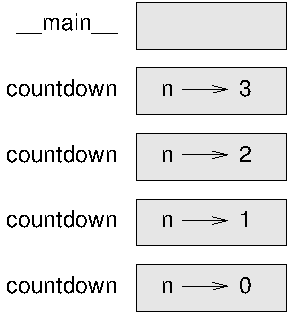
\includegraphics[scale=0.8]{figs/stack2.pdf}}
\caption{栈图.}
\label{fig.stack2}
\end{figure}

通常, 最顶层的框属于\verb"__main__". 
其为空, 是因为没有在\verb"__main__"内创建变量或者传入参数. 
\index{base case}
\index{recursion!base case}

四个{\tt countdown}的框分别对应不同的{\tt n}值, 最底层{\tt n=0}的栈, 叫做
{\tt 边界条件},  也就是不再进行递归调用的栈, 所以下面也不会再有其他框了. 

做个练习, 以\verb"s = 'Hello'"和{\tt n=2}为参数, 绘制调用\verb"print_n"的栈图. 
然后编写名为\verb"do_n"的函数, 参数为一个函数对象, 和一个数值{\tt n}. 
使其调用{\tt n}次给定的函数. 


\section{无穷递归}
\index{infinite recursion}
\index{recursion!infinite}
\index{runtime error}
\index{error!runtime}
\index{traceback}

如果递归一直无法触及边界条件, 则会一直调用, 永不终止. 
这便叫做{\bf 无穷递归}, 出现这种情况, 往往表示情况不妙. 
下面是个无穷递归的极简程序:

\begin{verbatim}
def recurse():
    recurse()
\end{verbatim}
%
多数编程环境中, 无穷递归的程序不会一直运行. 
当达到了最大递归深度, Python便会报错:
\index{exception!RuntimeError}
\index{RuntimeError}

\begin{verbatim}
  File "<stdin>", line 2, in recurse
  File "<stdin>", line 2, in recurse
  File "<stdin>", line 2, in recurse
                  .   
                  .
                  .
  File "<stdin>", line 2, in recurse
RuntimeError: Maximum recursion depth exceeded
\end{verbatim}
%
这次的追踪信息比以往的要长一些. 这个错误发生时, 栈中已经有1000个{\tt 递归}框了!

如若不幸遇到无穷递归, 最好重新审视一下你的函数, 确保存在不再进行递归调用的边界条件. 
如果已有边界条件, 请检查是否可以保证其被触达. 


\section{键盘输入}
\index{keyboard input}

到目前为止, 我们编写的程序,基本都没有涉及用户输入, 它们每次执行都一样. 

Python提供了内置函数{\tt input}, 可以暂停程序运行, 等待用户键入信息. 
当用户敲击{\sf  Return} 或 {\sf Enter}键时, 程序恢复运行, 
同时\verb"input"将用户输入作为字符串返回. 
在Python 2中, 同样作用的函数叫做\verb"raw_input".
\index{Python 2}
\index{input function}
\index{function!input}

\begin{verbatim}
>>> text = input()
What are you waiting for?
>>> text
'What are you waiting for?'
\end{verbatim}
%
在接收用户输入时, 最好给用户以提示, 使其知晓要输入的内容. 
\verb"input"会把参数作为提示信息:
\index{prompt}

\begin{verbatim}
>>> name = input('What...is your name?\n')
What...is your name?
Arthur, King of the Britons!
>>> name
'Arthur, King of the Britons!'
\end{verbatim}
%
提示信息末尾的\verb"\n"是个{\bf 换行符}, 表示另起一行的特殊字符. 
所以用户的输入信息会处于提示信息下面.  
\index{newline}

若想得到一个整数, 便要将返回值转为{\tt int}:

\begin{verbatim}
>>> prompt = 'What...is the airspeed velocity of an unladen swallow?\n'
>>> speed = input(prompt)
What...is the airspeed velocity of an unladen swallow?
42
>>> int(speed)
42
\end{verbatim}
%
但如果用户输入的不是数字类型的字符串, 那便要报错了:

\begin{verbatim}
>>> speed = input(prompt)
What...is the airspeed velocity of an unladen swallow?
What do you mean, an African or a European swallow?
>>> int(speed)
ValueError: invalid literal for int() with base 10
\end{verbatim}
%
后续我们会学习如何应对这种错误. 
\index{ValueError}
\index{exception!ValueError}


\section{调试}
\label{whitespace}
\index{debugging}
\index{traceback}

当遇到语法异常或者运行时异常, 其报错信息详细而充分, 
但会令人无所适从. 一般最有用的也就下面两部分:

\begin{itemize}

\item 哪种错误

\item 出于何处

\end{itemize}

语法错误通常容易定位, 但是有些情况需要注意. 
空格异常可能比较棘手, 因为空格和制表({\tt Tab})符是不可见的, 所以容易被忽视. 
\index{whitespace}

\begin{verbatim}
>>> x = 5
>>>  y = 6
  File "<stdin>", line 1
    y = 6
    ^
IndentationError: unexpected indent
\end{verbatim}
%
此例中, 问题在于, 第二行多了一个空格. 
但是错误信息指向 {\tt y}, 便误导了我们. 
通常, 错误信息只标识错误发生的位置, 但是问题代码可能在
此位置之前, 甚至是前行代码. 
\index{error!runtime}
\index{runtime error}

运行时错误也如此, 假设你要计算分贝的信噪比. 
公式是$SNR_{db} = 10 \log_{10} (P_{signal} / P_{noise})$. 
在Python中, 编码如下:

\begin{verbatim}
import math
signal_power = 9
noise_power = 10
ratio = signal_power // noise_power
decibels = 10 * math.log10(ratio)
print(decibels)
\end{verbatim}
%
运行代码, 会遇到报错:
%
\index{exception!OverflowError}
\index{OverflowError}

\begin{verbatim}
Traceback (most recent call last):
  File "snr.py", line 5, in ?
    decibels = 10 * math.log10(ratio)
ValueError: math domain error
\end{verbatim}
%
错误信息显示, 问题出在第5行, 
但是这行代码看不出任何问题. 
为了确定具体问题, 可以输出{\tt ratio}值, 显示是0.
那问题便出在第4行, 本应使用浮点数除法, 却误用了整除.
\index{floor division}
\index{division!floor}

对错误信息要仔细阅读, 但也不能完全偏信. 


\section{术语表}

\begin{description}


\item[向下取整(floor division):] 运算符{\tt //}, 将两数相除, 结果向下(负无穷方向)取整.
  \index{floor division} 
  \index{division!floor}

\item[求模运算符(modulus operator):]  一个运算符, 用百分号({\tt \%})表示, 作用于整数并返回两数相除后的余数. 
\index{modulus operator}
\index{operator!modulus}

\item[布尔表达式(boolean expression):]  结果为{\tt True} 或 {\tt False}的表达式.
\index{boolean expression}
\index{expression!boolean}

\item[关系运算符(relational operator):] 比较操作数的运算符, 包括 
{\tt ==}, {\tt !=}, {\tt >}, {\tt <}, {\tt >=} 和 {\tt <=}.

\item[逻辑运算符(logical operator):] 组合布尔表达式的运算符, 包括 
{\tt and}, {\tt or} 以及 {\tt not}.

\item[条件语句(conditional statement):]  根据条件, 确定程序运行流程的语句.
\index{conditional statement}
\index{statement!conditional}

\item[条件(condition):] 条件语句中的布尔表达式, 确定分支走向.
\index{condition}

\item[复合语句(compound statement):]  由头部和缩进体构成的语句, 头部以冒号(:)结尾, 
缩进体相对头部需要缩进.
\index{compound statement}

\item[分支(branch):] 条件语句中一个可选的语句序列. 
\index{branch}

\item[链式条件(chained conditional):] 一系列可选分支构成的条件语句. 
\index{chained conditional}
\index{conditional!chained}

\item[嵌套条件(nested conditional):] 出现在条件语句的分支中的条件语句. 
\index{nested conditional}
\index{conditional!nested}

\item[返回语句(return statement):] 令函数立刻结束并返回给调用方的语句. 
\index{return statement}

\item[递归(recursion):]  函数调用自身的过程. 
\index{recursion}

\item[边界条件(base case):]  递归函数中不再进行递归调用的条件. 
\index{base case}

\item[无穷递归(infinite recursion):]  不存在或者永远无法触及边界条件的递归, 最终, 无穷递归会报运行时异常.
\index{infinite recursion}

\end{description}

\section{习题集}

\begin{exercise}

{\tt time}模块提供同样名为{\tt time}的函数, 此函数以某个``时间点''为基准, 
返回当前格林威治时间戳. 在Unix系统中, 
一般以1970年1月1日为参考``时间点''. 

\begin{verbatim}
>>> import time
>>> time.time()
1437746094.5735958
\end{verbatim}

编写一个脚本, 读取当前时间并将其转换为日期时间(以时分秒格式表示), 
以及基准时间点以来的天数. 

\end{exercise}


\begin{exercise}
\index{Fermat's Last Theorem}

费马大定理表明, 不存在任何正整数
$a$, $b$, 和 $c$ 满足

\[ a^n + b^n = c^n \]
%
当$n$大于2时.

\begin{enumerate}

\item 编写函数 \verb"check_fermat" , 它接受四个入参---{\tt a}, {\tt b}, {\tt c} 和 {\tt n}---
并检验费马大定理是否成立. 
如果$n$大于2同时满足

\[a^n + b^n = c^n \]
%
那么程序应输出, ``Holy smokes, Fermat was wrong!'', 
否则, 输出``No, that doesn't work.''

\item 编写一个函数, 提示用户输入 {\tt a}, {\tt b}, {\tt c} 和 {\tt n}, 
并将其转换为整数, 然后用\verb"check_fermat" 来检验它们是否违背了费马大定理. 

\end{enumerate}

\end{exercise}


\begin{exercise}
\index{triangle}

给你三根木棍, 你可能无法将其拼成三角形, 比如, 一根12英寸长, 
其余两根1英寸长, 这两根太短, 以至于都到不了长的那根的中间. 
所以, 对于三根任意长度的木棍, 都有一个简单方法, 可以确定其是否可以拼成三角形:

\begin{quotation}
三根木棍中, 如果有任意一根长度大于另外两根之和, 则无法组成三角形. 
否则, 便可以拼成三角形. (如果两边之和等于第三边, 便称其为``退化''三角形. )
\end{quotation}

\begin{enumerate}

\item 编写\verb"is_triangle" 函数, 以三个整数变量为入参, 
同时根据三个特定长度的木棍是否可以拼成三角形, 来输出 ``Yes'' 或 ``No''. 

\item 编写一个函数, 提示用户输入三个木棍的长度, 并将其转换为整数, 
并使用\verb"is_triangle"函数检测这三个值是否可以拼成三角形. 
\end{enumerate}

\end{exercise}

\begin{exercise}
下面的程序会输出什么? 绘制栈图, 展示输出结果时的程序状态.

\begin{verbatim}
def recurse(n, s):
    if n == 0:
        print(s)
    else:
        recurse(n-1, n+s)

recurse(3, 0)
\end{verbatim}

\begin{enumerate}

\item 如果像这样{\tt  recurse(-1, 0)}, 调用函数会发生什么?

\item 为此函数编写帮助文档, 告知使用函数所须了解的相关信息(仅此而已).

\end{enumerate}

\end{exercise}

以下练习需要用到第~\ref{turtlechap}节提到的{\tt turtle}模块:
\index{turtle module}

\begin{exercise}
阅读下面函数, 看看是否能明白其功能(参阅第~\ref{turtlechap}节的案例). 
运行并看看是否理解正确. 

\begin{verbatim}
def draw(t, length, n):
    if n == 0:
        return
    angle = 50
    t.fd(length*n)
    t.lt(angle)
    draw(t, length, n-1)
    t.rt(2*angle)
    draw(t, length, n-1)
    t.lt(angle)
    t.bk(length*n)
\end{verbatim}

\end{exercise}


\begin{figure}
\centerline
{
\includegraphics[scale=0.8]{figs/koch.pdf}}
\caption{科赫曲线.}
\label{fig.koch}
\end{figure}

\begin{exercise}
\index{Koch curve}

科赫曲线(The Koch curve)是类似图~\ref{fig.koch}的一种分形几何. 
要想绘制长度为$x$的曲线, 你需要如此这般:

\begin{enumerate}

\item 绘制长为$x/3$的科赫曲线. 

\item 左转60度. 

\item 继续绘制长 $x/3$的曲线. 

\item 右转120度. 

\item 再绘制长 $x/3$的曲线. 

\item 左转60度. 

\item 绘制长为 $x/3$的曲线. 

\end{enumerate}

当$x$小于3时, 会有所不同: 在此情况下, 绘制所得为长$x$的一段直线. 

\begin{enumerate}

\item 编写{\tt koch}函数, 以 turtle 和长度length为参数, 使用turtle, 根据指定长度, 绘制
科赫曲线. 

\item 编写{\tt snowflake}函数, 使其绘制三条科赫曲线, 
从而构成雪花的轮廓.

参阅: \url{http://thinkpython2.com/code/koch.py}.

\item 生成科赫曲线有多种方法. 参看
\url{http://en.wikipedia.org/wiki/Koch_snowflake} 上的案例, 选择你喜欢的进行实现. 


\end{enumerate}
\end{exercise}


\chapter{有值返回函数}
\label{fruitchap}

目前我们用到的很多Python函数都有返回值, 比如math函数. 
但我们目前写的函数, 都是无返回值的: 它们只是实现特定的效果, 比如输出值, 
或者移动小乌龟, 只是它们都没有返回值. 
本章, 重点学习如何编写有值返回函数. 

\section{返回值}
\index{return value}

调用函数便会产生返回值, 一般我们将其赋值给变量或者作为表达式的一部分使用. 

\begin{verbatim}
e = math.exp(1.0)
height = radius * math.sin(radians)
\end{verbatim}
%
目前写的函数, 多是无返回值的. 笼统讲, 是没有返回值, 然而, 
更准确地说, 返回值是{\tt None}.

本章, 我们总算要写一些有返回值的函数了. 
第一个例子是 {\tt area}函数, 根据给定的半径, 返回面积:

\begin{verbatim}
def area(radius):
    a = math.pi * radius**2
    return a
\end{verbatim}
%
前面我们学过了{\tt return} 语句, 但是在有值返回的函数中, 
{\tt return} 语句包含表达式. 
其意思为:``立即将此表达式作为返回值进行返回. ''
鉴于表达式可简可繁, 上述函数可以精炼为下面样子:
\index{return statement}
\index{statement!return}

\begin{verbatim}
def area(radius):
    return math.pi * radius**2
\end{verbatim}
%
但是, 使用类似{\tt a}这样的{\bf 临时变量}, 更加清晰明了, 便于调试. 
\index{temporary variable}
\index{variable!temporary}

有时候, 根据条件设置多个不同返回语句, 更加高效:

\begin{verbatim}
def absolute_value(x):
    if x < 0:
        return -x
    else:
        return x
\end{verbatim}
%
这些{\tt return}语句位于条件语句的不同分支中, 而且, 只有一个会执行. 

一旦返回语句执行, 函数不再执行后续语句, 立刻终止运行. 
{\tt return}语句后的代码, 或者任何不被触及的代码, 都叫做{\bf 无效代码}.
\index{dead code}

有值返回函数中, 最好保证程序中的每种可能情况, 都有{\tt return}语句. 例如:

\begin{verbatim}
def absolute_value(x):
    if x < 0:
        return -x
    if x > 0:
        return x
\end{verbatim}
%

这个函数错误之处在于, 如果{\tt x}恰好是0,
便没有条件为真, 也就不会触及任何{\tt return}语句. 
如果运行到函数最后, 返回值将是{\tt None}, 而不是0的绝对值. 
\index{None special value}
\index{special value!None}

\begin{verbatim}
>>> print(absolute_value(0))
None
\end{verbatim}
%
顺便提一下, Python提供了内置函数{\tt abs}来计算绝对值. 
\index{abs function}
\index{function!abs}

做个练习, 编写 {\tt compare} 函数, 输入为{\tt x} 和 {\tt y}, 
如果 {\tt x > y},  返回 {\tt 1}, 
如果{\tt x == y},  返回{\tt 0} , 
如果 {\tt x < y},  返回{\tt -1}. 
\index{compare function}
\index{function!compare}


\section{增量开发}
\label{incremental.development}
\index{development plan!incremental}

随着编写的函数越来越长, 你会发现, 调试时间也越来越恐怖. 

为了处理越来越复杂的程序, 您可能想尝试一种新的方法, 即{\bf 增量开发}.
增量开发的目标是通过每次只添加并测试少量代码, 从而避免
长时间的连续开发调试. 
\index{testing!incremental development}
\index{Pythagorean theorem}

比如, 若想得到两坐标 $(x_1, y_1)$ 和 $(x_2, y_2)$之间的距离, 
根据勾股定理, 距离为:

\begin{displaymath}
\mathrm{distance} = \sqrt{(x_2 - x_1)^2 + (y_2 - y_1)^2}
\end{displaymath}
%
首先考虑在Python中 {\tt distance}函数是什么样子. 换句话说, 就是何为输入(形参), 
何为输出(返回值)?

此例中, 输入为两个点, 即四个值表示的坐标. 返回值为两点的距离, 用浮点数表示. 

你可以立刻写出函数的大致轮廓:

\begin{verbatim}
def distance(x1, y1, x2, y2):
    return 0.0
\end{verbatim}
%
显然, 这个版本无法计算距离, 因为其总是返回0.
但是, 它的语法正确, 同时可以运行, 
这意味着, 在其变复杂之前, 你能够对其进行测试. 

用实例参数调用此函数, 看看效果:

\begin{verbatim}
>>> distance(1, 2, 4, 6)
0.0
\end{verbatim}
%
选择这些值作为坐标, 是因为其水平距离是3,垂直距离是4,两点距离便是5, 
也就是3-4-5直角三角形的斜边. 
在测试函数过程中, 知道预期结果, 尤为重要. 
\index{testing!knowing the answer}

我们已经确认此函数语法正确, 现在便可以向函数体添加代码了. 
合理的下一步是计算$x_2 - x_1$ 和 $y_2 - y_1$的值, 
下一个版本会将其保存为临时变量, 并输出. 

\begin{verbatim}
def distance(x1, y1, x2, y2):
    dx = x2 - x1
    dy = y2 - y1
    print('dx is', dx)
    print('dy is', dy)
    return 0.0
\end{verbatim}
%
如果函数正常, 则会输出\verb"dx is 3" 和 \verb"dy is 4". 
这样, 我们便知道函数入参正确, 同时前期的计算无误. 
如果发生异常, 那么我们只需要仔细检查这几行代码. 

接下来, 我们计算{\tt dx} 和 {\tt dy}的平方和:

\begin{verbatim}
def distance(x1, y1, x2, y2):
    dx = x2 - x1
    dy = y2 - y1
    dsquared = dx**2 + dy**2
    print('dsquared is: ', dsquared)
    return 0.0
\end{verbatim}
%
同样, 你要在此阶段运行代码, 并检查输出(输出值应为25). 
最后, 你可以使用{\tt math.sqrt}来计算并返回结果:
\index{sqrt}
\index{function!sqrt}

\begin{verbatim}
def distance(x1, y1, x2, y2):
    dx = x2 - x1
    dy = y2 - y1
    dsquared = dx**2 + dy**2
    result = math.sqrt(dsquared)
    return result
\end{verbatim}
%
如果运行正常, 意味着程序正确. 
否则, 就要在返回语句前打印{\tt result}的值, 仔细排查. 

最终版本的函数, 除了返回一个值, 不会输出任何信息. 
{\tt print} 语句只是为了便于调试代码, 一旦确认程序无误, 就应将其移除. 
这种代码, 一般叫做{\bf 脚手架},  主要用来辅助构建程序, 而不应
忝列最终成品之中. 
\index{scaffolding}

开始时, 一般每次只增加一两行代码. 但随着经验增长, 慢慢你便可以驾驭大段代码了. 
无论如何, 增量开发都能节约大量调试时间.

此方法的关键在于:

\begin{enumerate}

\item 从一个小的可运行程序开始, 并进行小的增量变化. 任何时候遇到错误, 都要弄清缘由, 尽快解决. 

\item 利用变量保存中间值, 以便展示和检验. 

\item 一旦程序运行正常, 便可以移除脚手架代码, 或将多个语句合并为复合表达式, 从而精简代码. 
但前提是不会令代码难以阅读. 

\end{enumerate}

做个练习, 用增量开发的方式, 写个函数{\tt hypotenuse}, 
给定直角三角形的两个直角边, 返回斜边长度. 
同时在开发过程中记录各个阶段的进展. 
\index{hypotenuse}


\section{组合}
\index{composition}
\index{function composition}

如你所想, 你可以在一个函数中调用另外的函数. 
例如, 编写一个函数, 其接收两个坐标, 一个是圆心, 一个是圆周上的点, 
计算圆的面积. 

假设圆心坐标为变量{\tt xc} 和
{\tt yc}, 圆周上点的坐标为{\tt xp} 和 {\tt yp}.
首先要计算圆的半径, 也就是两点之间的距离. 
便可以借用之前写过的 {\tt distance}的函数, 如下:

\begin{verbatim}
radius = distance(xc, yc, xp, yp)
\end{verbatim}
%
下一步便是根据半径, 计算面积, 我们刚刚也写过:

\begin{verbatim}
result = area(radius)
\end{verbatim}
%
将上述步骤封装在一个函数中, 我们得到:
\index{encapsulation}

\begin{verbatim}
def circle_area(xc, yc, xp, yp):
    radius = distance(xc, yc, xp, yp)
    result = area(radius)
    return result
\end{verbatim}
%
临时变量{\tt radius} 和 {\tt result} 在开发和调试时有用, 但是程序一旦正常运行, 
便可以通过组合函数调用, 使其更简洁:

\begin{verbatim}
def circle_area(xc, yc, xp, yp):
    return area(distance(xc, yc, xp, yp))
\end{verbatim}
%

\section{布尔函数}
\label{boolean}

函数可以返回布尔值, 从而便于隐藏函数内复杂的判断逻辑.  \index{boolean function}
例如:

\begin{verbatim}
def is_divisible(x, y):
    if x % y == 0:
        return True
    else:
        return False
\end{verbatim}
%
给布尔函数命名, 通常采用类似是/否提问的词语; 
\verb"is_divisible" 返回{\tt True}或{\tt False}, 
以标识{\tt x}是否可以被{\tt y}整除. 

这是个示例:

\begin{verbatim}
>>> is_divisible(6, 4)
False
>>> is_divisible(6, 3)
True
\end{verbatim}
%
既然{\tt ==}运算符的结果为布尔值, 
我们便可以直接返回, 从而精简函数:

\begin{verbatim}
def is_divisible(x, y):
    return x % y == 0
\end{verbatim}
%
布尔函数一般用于条件语句:
\index{conditional statement}
\index{statement!conditional}

\begin{verbatim}
if is_divisible(x, y):
    print('x is divisible by y')
\end{verbatim}
%
也可以这么写:

\begin{verbatim}
if is_divisible(x, y) == True:
    print('x is divisible by y')
\end{verbatim}
%
但这个比较就显得多余了.

做个练习, 编写函数\verb"is_between(x, y, z)", 
如果$x \le y \le z$, 返回{\tt True}, 否则返回{\tt False}.


\section{再说递归}
\label{more.recursion}
\index{recursion}
\index{Turing complete language}
\index{language!Turing complete}
\index{Turing, Alan}
\index{Turing Thesis}

目前, 我们只学到了Python的一小部分, 但麻雀虽小, 五脏俱全, 
这一小部分便足以表达一门{\em 完整的}编程语言了, 
也就是说, 如果一切皆是计算, 那么以上所学便已足够. 
任何程序都可以只用以上所学模块, 进行构建(当然, 可能还需要一些控制设备
的命令, 比如管理鼠标, 硬盘等, 但是也仅需要这些).

最早证明了上述伟大结论的是艾兰图灵(Alan Turing), 最早的计算机科学家之一
(有人会计较其是数学家, 但是早期的计算机科学家, 起初都是数学家). 
因此, 这个理论也叫做图灵论断(Turing Thesis). 
关于图灵论断, 如果想更加详细深入了解, 我推荐 Michael Sipser 所写
 {\em 计算理论导引(Introduction to the Theory of Computation)} 一书.

为了展示目前所学的威力, 我们分析几个递归数学函数. 
递归定义类似于循环定义, 某种意义上说, 函数定义体内包含了对定义体的引用. 
通常一个完全循环的定义, 是无用的:

\begin{description}

\item[致命的:] 一个形容词, 用来描述一些致命的东西.
\index{vorpal}
\index{circular definition}
\index{definition!circular}

\end{description}

如果在辞典中看到这样的定义, 可能会感到恼火. 
但你如果查询一下用符号$!$表示的阶乘函数的定义, 
可能会看到以下内容:
%
\begin{eqnarray*}
&&  0! = 1 \\
&&  n! = n (n-1)!
\end{eqnarray*}
%
这个定义声明0的阶乘为1, 同时对于任意$n$, 阶乘$n$等于$n$乘以阶乘$n-1$. 

所以$3!$等于3乘以$2!$,  而$2!$等于2乘以$1!$, $1!$又是1乘以
$0!$. 整理一下, $3!$ 等于3乘以2乘以1再乘以1,结果是6.
\index{factorial function}
\index{function!factorial}
\index{recursive definition}

如果你可以写出某个东西的递归定义, 那便可以编写个Python程序来计算它. 
首先要确定参数. 很显然, 此处{\tt factorial}函数的参数为整数:

\begin{verbatim}
def factorial(n):
\end{verbatim}
%
如果参数恰好为0, 只需要返回1:

\begin{verbatim}
def factorial(n):
    if n == 0:
        return 1
\end{verbatim}
%
而其他情况就有意思了, 需要递归调用以找到$n-1$的阶乘, 然后将其与
$n$相乘:

\begin{verbatim}
def factorial(n):
    if n == 0:
        return 1
    else:
        recurse = factorial(n-1)
        result = n * recurse
        return result
\end{verbatim}
%
此程序的执行流程和第~\ref{recursion}节的{\tt
countdown}极为相似. 如果以3为参数调用{\tt factorial}:

3不等于0,则走第二分支, 计算{\tt n-1}的阶乘...

\begin{quote}
2不等于0,则走第二分支, 计算{\tt n-1}的阶乘...


  \begin{quote}
 1不等于0,则走第二分支, 计算{\tt n-1}的阶乘...


    \begin{quote}
   0等于0, 则走第一分支, 不再递归调用, 返回1.
    \end{quote}

  返回值1乘以$n$, 而$n$此时为1,则返回1. 
  \end{quote}

返回值1乘以$n$, 此时$n$为2, 返回为2的结果.
\end{quote}

返回值(2)乘以此时为3的$n$, 结果为6, 也就是整个流程最终的结果. 
\index{stack diagram}

图~\ref{fig.stack3} 是这一系列函数调用的栈图展现.

\begin{figure}
\centerline
{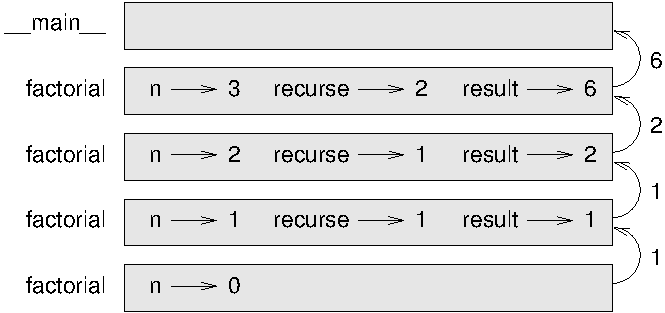
\includegraphics[scale=0.8]{figs/stack3.pdf}}
\caption{栈图.}
\label{fig.stack3}
\end{figure}

返回值会在栈中被传递. 
每个框内, 返回值就是{\tt result}的值, 也就是{\tt recurse}和{\tt n}相乘的结果. 
\index{function frame}
\index{frame}

最后的框中, 没有局部变量{\tt recurse}和{\tt result} , 是因为
创建它们的分支没有执行. 

\section{置信迁移}
\index{recursion}
\index{leap of faith}

阅读程序的一种方式是跟踪其执行顺序, 但是你很快会不堪重负. 
另一种可行方案, 我称之为``置信迁移''. 当遇到某个函数调用时, 
不是根据执行流程深入跟踪, 
而是{\em 假设}这个函数工作正常, 可以返回正确结果. 

实际当你使用内置函数时, 就已经在实践置信迁移了. 调用
{\tt math.cos} 或 {\tt math.exp}时, 并不会查看其具体实现. 
这是因为你相信写出这些内置函数的人是优秀的编程人员, 
所以相信这些函数可以正确运行. 

对于你来说, 调用自己的函数也是同理. 例如第~\ref{boolean}节, 
我们编写了\verb"is_divisible"函数, 用来判断一个数是否可以被另一个数
整除. 如果我们确信这些函数是正确的--代码检查以及测试都通过--
我们便可以直接使用它, 而无需再探究细节. 
\index{testing!leap of faith}

递归程序也一样. 当你进行递归调用时, 
无需一步步跟踪执行流程, 而是假设递归调用工作正常
(会返回正确的结果), 然后问问自己, ``既然我可以计算出 $n-1$的阶乘, 那么
是不是我也可以计算出$n$的阶乘?'' 很显然你可以, 乘以$n$即可. 

当然, 当你还没有完成函数编写, 便假设其正常运行, 是有点奇怪, 
所以这也是为何我们称其为置信迁移的原因!


\section{另例}
\label{one.more.example}

\index{fibonacci function}
\index{function!fibonacci}
在了解{\tt 阶乘}之后, 我们要学习的是递归数学函数中最常见的用例, 
{\tt 斐波拉契数列}. 
其详细定义可参阅\url{http://en.wikipedia.org/wiki/Fibonacci_number}:
%
\begin{eqnarray*}
&& \mathrm{fibonacci}(0) = 0 \\
&& \mathrm{fibonacci}(1) = 1 \\
&& \mathrm{fibonacci}(n) = \mathrm{fibonacci}(n-1) + \mathrm{fibonacci}(n-2)
\end{eqnarray*}
%
翻译为Python代码, 代码如下:

\begin{verbatim}
def fibonacci(n):
    if n == 0:
        return 0
    elif  n == 1:
        return 1
    else:
        return fibonacci(n-1) + fibonacci(n-2)
\end{verbatim}
%
若你尝试跟踪其流转, 那即使一个很小的$n$值, 都能令你头疼. 
但是, 基于置信迁移, 如果假设两个递归调用都运行正常, 那么很显然, 
将其相加, 便能得到正确结果. 
\index{flow of execution}


\section{类型检查}
\label{guardian}

试试调用{\tt factorial}函数并将1.5作为参数传递, 会发生什么?
\index{type checking}
\index{error checking}
\index{factorial function}
\index{RuntimeError}

\begin{verbatim}
>>> factorial(1.5)
RuntimeError: Maximum recursion depth exceeded
\end{verbatim}
%
看起来陷入了无限递归. 怎么会这样? 此函数有个边界条件--当 {\tt n == 0}时. 
但如果{\tt n}不是整数, 那便会{\em 掠过}边界条件, 一直递归下去. 
\index{infinite recursion}
\index{recursion!infinite}

第一次递归调用中, { \tt n}是0.5. 
下一次, 变成了-0.5.再然后, 会越来越小(更小的负数), 
也就永远不可能再成为0.

我们有两种方案. 一种是尝试改进{\tt factorial}函数, 使其支持浮点数, 
或者使其检验其参数类型. 
第一种方案会写出伽玛函数, 超出了本书的范畴. 所以选择方案二. 
\index{gamma function}

我们可以使用内置函数{\tt isinstance}来检验参数类型. 
同时, 我们也需要确保参数是正数:
\index{isinstance function}
\index{function!isinstance}

\begin{verbatim}
def factorial(n):
    if not isinstance(n, int):
        print('Factorial is only defined for integers.')
        return None
    elif n < 0:
        print('Factorial is not defined for negative integers.')
        return None
    elif n == 0:
        return 1
    else:
        return n * factorial(n-1)
\end{verbatim}
%
第一个边界条件, 针对非整数;
第二个, 则针对负整数. 
这两个边界条件中, 都会输出错误信息, 并返回{\tt None}, 
以标识运行错误:

\begin{verbatim}
>>> print(factorial('fred'))
Factorial is only defined for integers.
None
>>> print(factorial(-2))
Factorial is not defined for negative integers.
None
\end{verbatim}
% 
如果通过两个检验, 那可以确定$n$现在是非负整数, 
至此便可以确保递归会终止了. 
\index{guardian pattern}
\index{pattern!guardian}

此程序展示了一种叫做{\bf 哨兵}的角色. 
前两个条件, 就像哨兵一样, 避免程序犯错, 使其正确运行. 

在第~\ref{raise}节, 我们会看到一种更灵活的方案来输出错误信息: 上报异常. 


\section{调试}
\label{factdebug}
将程序大而化小, 也就天然地为调试创造了一个个的检查点. 
如果程序运行异常, 需要考虑以下三种可能原因:
\index{debugging} 

\begin{itemize}

\item 函数入参异常, 前置条件未满足. 

\item 函数本身异常, 后置条件不满足. 

\item 返回值或者调用方式异常. 

\end{itemize}

若要避免第一种异常, 可以在函数开头添加{\tt print}语句, 打印参数值(以及类型). 
或者编写代码, 显示校验前置条件. 
\index{precondition}
\index{postcondition}

如果参数没问题, 那在每个{\tt return}语句前, 增加{\tt print}语句, 打印返回值. 
如果可以的话, 最好手动检查结果. 同时尽量在调用函数时, 传入合适的参数, 
以使返回结果便于校验
(如第~\ref{incremental.development}节中所示). 

如果函数都正常, 那检验一下函数调用方式, 看看是否正确使用了返回值
(或者至少用到了返回值!)
\index{flow of execution}

在函数开头和结尾添加打印语句, 有助于更直观地观察执行流程. 例如, 下面是一个
带有打印语句的{\tt factorial}版本:

\begin{verbatim}
def factorial(n):
    space = ' ' * (4 * n)
    print(space, 'factorial', n)
    if n == 0:
        print(space, 'returning 1')
        return 1
    else:
        recurse = factorial(n-1)
        result = n * recurse
        print(space, 'returning', result)
        return result
\end{verbatim}
%
在此, 用{\tt 空格}字符串来控制输出语句的缩进. 以下为{\tt factorial(4)}的运行结果:

\begin{verbatim}
                 factorial 4
             factorial 3
         factorial 2
     factorial 1
 factorial 0
 returning 1
     returning 1
         returning 2
             returning 6
                 returning 24
\end{verbatim}
%
若惑于其函数执行流程, 那么, 此输出可能会有助于理解. 
有时候, 增加脚手架需要耗费一点时间, 
但是, 这一点时间的花费, 往往能够节约大量的调试时间. 

\section{术语表}

\begin{description}

\item[临时变量(temporary variable):] 复杂运算中, 暂存中间值的变量. 
\index{temporary variable}
\index{variable!temporary}

\item[无效代码(dead code):]  程序永远不会运行的语句, 通常出现在{\tt return}语句之后. 
\index{dead code}

\item[增量开发(incremental development):]  一种每次仅添加并测试少量代码的开发方案, 
小步慢跑, 从而避免调试. 
\index{incremental development}

\item[脚手架(scaffolding):]  程序开发中起辅助作用的代码, 但不会留在最终程序中. 
\index{scaffolding}

\item[哨兵(guardian):]  一种编程模式, 使用条件语句进行检验, 并处理可能导致异常的情形. 
\index{guardian pattern}
\index{pattern!guardian}

\end{description}


\section{习题集}

\begin{exercise}
针对以下代码, 绘制栈图, 查看程序输出为何?
\index{stack diagram}

\begin{verbatim}
def b(z):
    prod = a(z, z)
    print(z, prod)
    return prod

def a(x, y):
    x = x + 1
    return x * y

def c(x, y, z):
    total = x + y + z
    square = b(total)**2
    return square

x = 1
y = x + 1
print(c(x, y+3, x+y))
\end{verbatim}

\end{exercise}


\begin{exercise}
\label{ackermann}

阿克曼(Ackermann)函数$A(m, n)$定义如下:

\begin{eqnarray*}
A(m, n) = \begin{cases} 
              n+1 & \mbox{if } m = 0 \\ 
        A(m-1, 1) & \mbox{if } m > 0 \mbox{ and } n = 0 \\ 
A(m-1, A(m, n-1)) & \mbox{if } m > 0 \mbox{ and } n > 0.
\end{cases} 
\end{eqnarray*}
%
参考\url{http://en.wikipedia.org/wiki/Ackermann_function}.
编写{\tt ack}函数代码, 计算Ackermann函数. 
用此代码执行{\tt ack(3, 4)}, 结果应该为125. 
同时, 当{\tt m} 和{\tt n}较大时, 看看结果有何不同? 
答案参见:\url{http://thinkpython2.com/code/ackermann.py}.
\index{Ackermann function}
\index{function!ack}

\end{exercise}


\begin{exercise}
\label{palindrome}

像``noon''和``redivider''一样, 正序和倒序拼写方式完全一样的词, 称为回文词. 
从递归角度看, 如果开始和结束字母相同, 同时中间部分是回文词, 那么就可以认为
总体是回文词. 
\index{palindrome}
下文为返回字符串首字母, 尾字母以及中间字母的函数:

\begin{verbatim}
def first(word):
    return word[0]

def last(word):
    return word[-1]

def middle(word):
    return word[1:-1]
\end{verbatim}
%

在第~\ref{strings}节会详细解释其原理.

\begin{enumerate}

\item 将这些函数代码, 写入文件{\tt palindrome.py}, 并测试输出. 
用两个字母, 测试{\tt middle}函数, 看看会怎么样? 一个字母呢?  
尝试传入不包含任何字母的空字符串\verb"''",  会如何?

\item 编写\verb"is_palindrome"函数, 如果传入参数为回文字符串, 
则返回{\tt True}, 否则返回{\tt False}. 
提示一下, 你可以使用内置函数{\tt len}检验字符串长度. 

\end{enumerate}

答案参阅: \url{http://thinkpython2.com/code/palindrome_soln.py}.

\end{exercise}

\begin{exercise}

如果$a$可以被$b$整除, 同时$a/b$也是$b$的幂次方, 那么$a$便是$b$是幂次方. 
编写函数\verb"is_power", 
接收参数{\tt a}和{\tt b}, 如果{\tt a}是{\tt b}的幂次方, 则返回{\tt True}. 
提示:注意边界条件. 

\end{exercise}


\begin{exercise}
\index{greatest common divisor (GCD)}
\index{GCD (greatest common divisor)}

两个数$a$和$b$的最大公约数(GCD), 是指能同时被整除且没有余数的最大数. 

寻找最大公约数的一种方法便是基于观察, 如果$r$ 是$a$除以$b$的余数, 
那么$gcd(a, b) = gcd(b, r)$, 边界条件是$gcd(a, 0) = a$.

编写函数\verb"gcd", 接收参数{\tt a}和{\tt b}, 并返回其最大公约数. 


致谢: 此习题借鉴了Abelson和
Sussman的{\em Structure and Interpretation of Computer Programs}中的样例.

\end{exercise}


\chapter{迭代}

本章主讲迭代, 其主要实现重复执行一组语句. 
在第~\ref{recursion}节的递归, 便是一种迭代. 
在第~\ref{repetition}节的{\tt for}循环, 也是一种迭代. 
本章, 我们会接触另一种迭代, {\tt while} 语句. 
但这里要先讲一下变量赋值. 

\section{重新赋值}
\index{assignment}
\index{statement!assignment}
\index{reassignment}

你可能已经注意到, 相同的变量可以被多次赋值. 
重新赋值会将已存在的变量指向新的值(并且不再指向旧的值).

\begin{verbatim}
>>> x = 5
>>> x
5
>>> x = 7
>>> x
7
\end{verbatim}
%
第一次输出{\tt x}, 值为5, 第二次输出, 值为7.

图~\ref{fig.assign2}展示了栈图中{\bf 重新赋值}
的过程. \index{state diagram} \index{diagram!state}

在此, 我想澄清一下大家的困惑.
因为Python使用等号({\tt =})进行赋值, 
很容易将{\tt a = b}这样的语句, 作为数学命题中的等式进行解读, 
认为其表示{\tt a}和{\tt b}相等. 
这种解读是极其错误的. 
\index{equality and assignment}

首先, 等式是对称关系, 而赋值不是. 
例如, 数学中, 如果$a=7$, 那么$7=a$. 但是在Python中, 
{\tt a = 7}正确, 但是{\tt 7 = a}则不然. 

同样, 在数学领域, 等式结果要么真要么假. 
如果$a=b$成立, 那么 $a$始终等于$b$. 
而在Python中, 虽然赋值语句可以使两变量相等, 但是无法保证其一直相等:

\begin{verbatim}
>>> a = 5
>>> b = a    # a 和 b 相等
>>> a = 3    # a 和 b 不等
>>> b
5
\end{verbatim}
%
第三行代码, 改变了{\tt a}的值, 但是没有改变{\tt b}, 所以他们不再相等. 

很多时候我们需要给变量重新赋值, 但是要谨慎使用. 
如果变量的值变动过于频繁, 代码后续将难以理解, 同时调试也困难. 

\begin{figure}
\centerline
{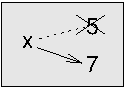
\includegraphics[scale=0.8]{figs/assign2.pdf}}
\caption{栈图}
\label{fig.assign2}
\end{figure}



\section{变量更新}
\label{update}

\index{update}
\index{variable!updating}

一种常见的重新赋值, 是{\bf 变量更新},
通常是基于前值进行修改而得到新值. 

\begin{verbatim}
>>> x = x + 1
\end{verbatim}
%
这句代码表示``获取{\tt x}的值, 然后加一, 得到新值, 继而用新值更新{\tt x}.'' 

如果你尝试更新未定义变量, 会遇到错误, 
因为Python会在赋值{\tt x} 前会先计算右侧表达式:

\begin{verbatim}
>>> x = x + 1
NameError: name 'x' is not defined
\end{verbatim}
%
更新变量前, 一定要先{\bf 初始化}, 通常采用简单赋值来实现:
\index{initialization (before update)}

\begin{verbatim}
>>> x = 0
>>> x = x + 1
\end{verbatim}
%
对变量进行加1来使其更新, 叫做{\bf 递增};
执行减1更新变量, 叫做{\bf 递减}. 
\index{increment}
\index{decrement}


\section{{\tt while}语句}
\index{statement!while}
\index{while loop}
\index{loop!while}
\index{iteration}
计算机通常用于自动化一些重复性工作. 
对于大量重复的相同或相似任务, 计算机可以永不犯错, 
这也是计算机精擅之处, 却恰恰是人类最不擅长的. 
在计算机编程中, 这种重复, 便称作{\bf 迭代}.

我们已经遇到过两个函数, {\tt countdown} 和
\verb"print_n",  它们都是使用递归进行迭代. 
因迭代操作很普遍, Python提供了一些内置功能来便捷使用. 
一个便是在第~\ref{repetition}节见到的{\tt for}语句, 我们后续再讲. 

另一个便是{\tt while}语句, 下面是{\tt countdown}的{\tt while}语句版本:

\begin{verbatim}
def countdown(n):
    while n > 0:
        print(n)
        n = n - 1
    print('Blastoff!')
\end{verbatim}
%
{\tt while}语句很容易理解, 因为其便如英语表达一样. 
意为, ``当{\tt n}大于0时, 打印{\tt n}值, 然后自减1.
直到当等于0时, 打印 {\tt Blastoff!}''
\index{flow of execution}

正式些讲, 下面是{\tt while}语句的执行流程:

\begin{enumerate}

\item 确定条件之真假.

\item 如果为假, 退出{\tt while}语句, 执行后续语句. 

\item 如果为真, 运行执行体, 回到第一步. 

\end{enumerate}

这种程序流转, 便叫做循环. 因为第三步骤时, 会返回到起点. 
\index{condition}
\index{loop}
\index{body}

循环体通常会修改一个或多个变量的值, 从而令条件最终为假, 终止循环. 
否则, 循环会一直重复, 成为{\bf 无限循环}. 
对计算机科学家们, 有个乐此不疲的玩笑, 
便是观察洗发水的使用说明, 
``起泡, 冲洗, 重复'',  这就是个无限循环. 
\index{infinite loop}
\index{loop!infinite}

在{\tt countdown}例子中, 我们如此来确保循环终止:
如果{\tt n}小于或等于0,循环不再运行. 
由于{\tt n}每循环一次, 就会变小, 终究会达到0.

而有些循环, 则不太容易判断是否会终止, 比如:

\begin{verbatim}
def sequence(n):
    while n != 1:
        print(n)
        if n % 2 == 0:        # n 是偶数
            n = n / 2
        else:                 # n 是奇数
            n = n*3 + 1
\end{verbatim}
%
此循环的条件是{\tt n != 1},  那么只有{\tt n}等于{\tt 1}时, 条件为假, 循环才终止. 

每次循环, 程序都输出{\tt n}的值, 然后检查是奇是偶. 
如果是偶数, 则{\tt n}除以2. 如果是奇数, 则{\tt n}值更新为{\tt n*3 + 1}. 
例如, 如果{\tt sequence}的参数为3, {\tt n}值依次变为3, 10, 5, 16, 8, 4, 2, 1.


由于{\tt n} 有时增加, 有时减少, 所以很难保证{\tt n}会达到1, 或者程序终止. 
对于某些特殊的{\tt n}值, 我们可以确信循环会终止. 
比如, 如果起始值是2的幂, 那么循环每次执行后{\tt n}都会是偶数, 直到最终成为1.
刚刚例子中得到的数列, 从16开始, 便是如此. 
\index{Collatz conjecture}

问题的难点在于, 是否可以证明对于{\em 所有}正数的{\tt n}, 程序都会结束. 
目前, 还没有人能证明或者证否此命题! 
(参阅 \url{http://en.wikipedia.org/wiki/Collatz_conjecture})

做个练习, 用迭代替换递归, 重写第~\ref{recursion}节的\verb"print_n"函数, 

\section{{\tt break}语句}
\index{break statement}
\index{statement!break}
有时, 想要出世, 就需要先入世, 只有进入循环体, 
才知道何时应当终止循环. 
这时, 我们可以用{\tt break}语句跳出循环. 

例如, 想要获取用户的输入, 直到用户输入{\tt done}为止, 可以这样写:

\begin{verbatim}
while True:
    line = input('> ')
    if line == 'done':
        break
    print(line)

print('Done!')
\end{verbatim}
%
循环条件为{\tt True}, 便会一直循环, 所以只有触及 break 语句, 才会跳出循环. 

每次循环, 都会打印尖括号来提示用户输入, 
如果用户输入了{\tt done}, {\tt break} 语句会终止循环. 
否则, 程序会打印用户的输入, 并进入下一轮循环. 
举个例子:

\begin{verbatim}
> not done
not done
> done
Done!
\end{verbatim}
%
这种写法在{\tt while}循环中很常见, 
因为你能够随时检验其条件(而不仅仅在头部验证), 
同时也可以主动地去终止循环(``当发生某种情况时停止''), 
而不是被动地等待结束(``一直执行, 直到发生某种情况停止'').


\section{平方根}
\label{squareroot}
\index{square root}

%Loops are often used in programs that compute
%numerical results by starting with an approximate answer and
%iteratively improving it.
在编程中, 循环通常用来进行数值计算, 通过近似值逼近真实值来实现. 
\index{Newton's method}

%For example, one way of computing square roots is Newton's method.
%Suppose that you want to know the square root of $a$.  If you start
%with almost any estimate, $x$, you can compute a better
%estimate with the following formula:
例如, 牛顿公式(Newton's method)便是一种计算平方根的方法. 
若要计算$a$的平方根, 可以先确定一个任意的估计值, $x$, 
然后通过下面公式, 得到一个更优的值:

\[ y = \frac{x + a/x}{2} \]
%
%For example, if $a$ is 4 and $x$ is 3:
比如, 如果$a$为 4, 且$x$为 3:

\begin{verbatim}
>>> a = 4
>>> x = 3
>>> y = (x + a/x) / 2
>>> y
2.16666666667
\end{verbatim}
%
%The result is closer to the correct answer ($\sqrt{4} = 2$).  If we
%repeat the process with the new estimate, it gets even closer:
结果很接近正确答案($\sqrt{4} = 2$).
如果我们用得到的近似值, 重复刚才的流程, 结果会更接近:

\begin{verbatim}
>>> x = y
>>> y = (x + a/x) / 2
>>> y
2.00641025641
\end{verbatim}
% After a few more updates, the estimate is almost exact:
多重复几次, 结果便更准确:
\index{update}

\begin{verbatim}
>>> x = y
>>> y = (x + a/x) / 2
>>> y
2.00001024003
>>> x = y
>>> y = (x + a/x) / 2
>>> y
2.00000000003
\end{verbatim}
%In general we don't know ahead of time how many steps it takes
%to get to the right answer, but we know when we get there
%because the estimate
%stops changing:
通常, 我们很难预知, 重复多少次, 才能得到正确结果. 
但是, 我们知道, 一旦结果不再改变, 便是停止的时候:

\begin{verbatim}
>>> x = y
>>> y = (x + a/x) / 2
>>> y
2.0
>>> x = y
>>> y = (x + a/x) / 2
>>> y
2.0
\end{verbatim}
%When {\tt y == x}, we can stop.  Here is a loop that starts
%with an initial estimate, {\tt x}, and improves it until it
%stops changing:
当{\tt y == x}时, 我们便可以停止循环了. 
下面的循环, 以估计值{\tt x}开始并不断逼近真实值, 在结果不再变化时终止:

\begin{verbatim}
while True:
    print(x)
    y = (x + a/x) / 2
    if y == x:
        break
    x = y
\end{verbatim}
%For most values of {\tt a} this works fine, but in general it is
%dangerous to test {\tt float} equality.
%Floating-point values are only approximately right:
%most rational numbers, like $1/3$, and irrational numbers, like
%$\sqrt{2}$, can't be represented exactly with a {\tt float}.
对于大部分的{\tt a}值, 此方法都有效. 
但涉及到{\tt 浮点数}等式, 便很麻烦. 
浮点值一般认为是近似正确:
大部分的有理数, 比如$1/3$, 
以及类似$\sqrt{2}$的无理数, 都无法用{\tt 浮点数}来精确表示. 
\index{floating-point}
\index{epsilon}

%Rather than checking whether {\tt x} and {\tt y} are exactly equal, it
%is safer to use the built-in function {\tt abs} to compute the
%absolute value, or magnitude, of the difference between them:
与其费劲比较 {\tt x} 和 {\tt y} 是否相等, 不如用{\tt abs}计算
其差值的绝对值大小:

\begin{verbatim}
    if abs(y-x) < epsilon:
        break
\end{verbatim}
%Where \verb"epsilon" has a value like {\tt 0.0000001} that
%determines how close is close enough.
其中\verb"epsilon"是一个值, 比如{\tt 0.0000001}, 用于确定两个值
多接近才是足够接近. 


%\section{Algorithms}
\section{算法}
\index{algorithm}


%Newton's method is an example of an {\bf algorithm}: it is a
%mechanical process for solving a category of problems (in this
%case, computing square roots).
牛顿公式可以认为是一种{\bf 算法}:
通过既定步骤来解决一类问题(此例中为计算平方根). 

%To understand what an algorithm is, it might help to start with
%something that is not an algorithm.  When you learned to multiply
%single-digit numbers, you probably memorized the multiplication table.
%In effect, you memorized 100 specific solutions.  That kind of
%knowledge is not algorithmic.
要理解何为算法, 先要明白什么不属于算法. 
当你学习乘法时, 往往需要记忆乘法表. 
实际, 你记忆了100个特定答案. 这种知识不属于算法. 


%But if you were ``lazy'', you might have learned a few
%tricks.  For example, to find the product of $n$ and 9, you can
%write $n-1$ as the first digit and $10-n$ as the second
%digit.  This trick is a general solution for multiplying any
%single-digit number by 9.  That's an algorithm!
但如果你想``偷懒'', 你可能会发现一些小技巧. 
比如, 你想计算$n$和9的乘积, 只需把$n-1$, 作为第一个数字. 
$10-n$作为第二个数字即可. 这个小技巧对于任何数字乘以9都有效. 
这便是算法!
\index{addition with carrying}
\index{carrying, addition with}
\index{subtraction!with borrowing}
\index{borrowing, subtraction with}

%Similarly, the techniques you learned for addition with carrying,
%subtraction with borrowing, and long division are all algorithms.  One
%of the characteristics of algorithms is that they do not require any
%intelligence to carry out.  They are mechanical processes where
%each step follows from the last according to a simple set of rules.
同样地, 你学过的进位加法, 借位减法, 以及长除法, 
都是算法. 这些算法的一个共性便是, 都无需费力思考. 
它们都是机械的过程, 
遵循简单的规则, 一步步操作, 便可得到结果. 

%Executing algorithms is boring, but designing them is interesting,
%intellectually challenging, and a central part of computer science.
执行算法固然无聊, 但其设计过程却既有趣又挑战智力, 
同时也是计算机科学的核心. 

%Some of the things that people do naturally, without difficulty or
%conscious thought, are the hardest to express algorithmically.
%Understanding natural language is a good example.  We all do it, but
%so far no one has been able to explain {\em how} we do it, at least
%not in the form of an algorithm.
有些事情, 对于人们来说很自然, 豪无难度, 且下意识便可完成, 
而算法却很难解决. 
比如, 理解自然语言. 我们所有人都能轻易做到, 
但目前为止, 还没有人能阐明我们是{\em 如何}理解的, 
更不用说用算法的形式来解释. 

%\section{Debugging}
\section{调试}
\label{bisectbug}

%As you start writing bigger programs, you might find yourself
%spending more time debugging.  More code means more chances to
%make an error and more places for bugs to hide.
随着程序代码规模的增长, 你会发现需要耗费更多时间在
调试上. 一般更多的代码, 也就意味着更多的出错机会, 
以及更多的潜在问题. 
\index{debugging!by bisection}
\index{bisection, debugging by}
%One way to cut your debugging time is ``debugging by bisection''.
%For example, if there are 100 lines in your program and you
%check them one at a time, it would take 100 steps.
一种有效节约调试时间的方法便是``二分调试''.
比如, 有100行代码, 逐行检查, 需要100个步骤. 

%Instead, try to break the problem in half.  Look at the middle
%of the program, or near it, for an intermediate value you
%can check.  Add a {\tt print} statement (or something else
%that has a verifiable effect) and run the program.
相反, 将程序对半切分. 找到程序的中间位置, 或者靠近中间的位置, 
以便从中间开始检查. 添加{\tt print}语句(或者其他可验证效果的东西), 
然后运行代码. 

%If the mid-point check is incorrect, there must be a problem in the
%first half of the program.  If it is correct, the problem is
%in the second half.
如果中间检查点出现异常, 那代码前半部分有问题. 
如果中间没有出错, 那么问题便在后半部分了. 

%Every time you perform a check like this, you halve the number of
%lines you have to search.  After six steps (which is fewer than 100),
%you would be down to one or two lines of code, at least in theory.
每次如此检验代码, 将待检验的代码行数不断减半. 大约六步之后(远远小于100步), 
理论上, 便只剩下一两行代码需要检查了. 

%In practice it is not always clear what
%the ``middle of the program'' is and not always possible to
%check it.  It doesn't make sense to count lines and find the
%exact midpoint.  Instead, think about places
%in the program where there might be errors and places where it
%is easy to put a check.  Then choose a spot where you
%think the chances are about the same that the bug is before
%or after the check.
实际上, 很难清晰界定``代码中间位置'', 同时也很难在其位置检验. 
所以没必要计较于行数, 执着于中点. 
反而, 你需要多思考代码的哪些位置容易出错, 哪些地方又容易验证. 
然后选择一个恰到好处的点, 进行验证. 



\section{术语表}

\begin{description}

%\item[reassignment:] Assigning a new value to a variable that
%already exists.
\item[重新赋值(reassignment):] 给已存在的变量分配一个新值的过程. 
\index{reassignment}

%\item[update:] An assignment where the new value of the variable
%depends on the old.
\item[变量更新(update):] 基于前值, 计算新值, 更新变量的过程. 
\index{update}

%\item[initialization:] An assignment that gives an initial value to
%a variable that will be updated.
\item[初始化(initialization):] 给变量赋初始值, 以待后续更新. 
\index{initialization!variable}

%\item[increment:] An update that increases the value of a variable
%(often by one).
\item[递增(increment):] 使变量的值增加的更新操作(通常为1). 
\index{increment}


%\item[decrement:] An update that decreases the value of a variable.
\item[递减(decrement):] 使变量的值减少的更新操作. 
\index{decrement}

%\item[iteration:] Repeated execution of a set of statements using
%either a recursive function call or a loop.
\item[迭代(iteration):] 采用递归或者循环, 重复执行一段语句. 
\index{iteration}

%\item[infinite loop:] A loop in which the terminating condition is
%never satisfied.
\item[无限循环(infinite loop):] 终止条件一直不能抵达的循环. 
\index{infinite loop}

%\item[algorithm:]  A general process for solving a category of
%problems.
\item[算法(algorithm):]  解决一类问题的通用过程. 
\index{algorithm}

\end{description}

%\section{Exercises}
\section{习题集}

\begin{exercise}
\index{algorithm!square root}

%Copy the loop from Section~\ref{squareroot}
%and encapsulate it in a function called
%\verb"mysqrt" that takes {\tt a} as a parameter, chooses a
%reasonable value of {\tt x}, and returns an estimate of the square
%root of {\tt a}.  \index{encapsulation}
复制第~\ref{squareroot}节的循环, 封装为\verb"mysqrt" 函数, 
令其以{\tt a}为参数, 选择一个合适的值{\tt x}, 返回{\tt a}的
近似平方根.  \index{encapsulation}

%To test it, write a function named \verb"test_square_root"
%that prints a table like this:
若要测试, 需要编写一个名为\verb"test_square_root"的函数, 
输出下面的表格:

\begin{verbatim}
a   mysqrt(a)     math.sqrt(a)  diff
-   ---------     ------------  ----
1.0 1.0           1.0           0.0
2.0 1.41421356237 1.41421356237 2.22044604925e-16
3.0 1.73205080757 1.73205080757 0.0
4.0 2.0           2.0           0.0
5.0 2.2360679775  2.2360679775  0.0
6.0 2.44948974278 2.44948974278 0.0
7.0 2.64575131106 2.64575131106 0.0
8.0 2.82842712475 2.82842712475 4.4408920985e-16
9.0 3.0           3.0           0.0
\end{verbatim}
%
%The first column is a number, $a$; the second column is the square
%root of $a$ computed with \verb"mysqrt"; the third column is the
%square root computed by {\tt math.sqrt}; the fourth column is the
%absolute value of the difference between the two estimates.
第一列是数值$a$; 第二列是 \verb"mysqrt"函数计算出的$a$的平方根;
第三列是通过{\tt math.sqrt}计算出的平方根;
第四列是两者的差值绝对值. 
\end{exercise}


\begin{exercise}
\index{eval function}
\index{function!eval}
%The built-in function {\tt eval} takes a string and evaluates
%it using the Python interpreter.  For example:
内置函数{\tt eval}以字符串为输入, 并用Python解释器执行. 
如下:

\begin{verbatim}
>>> eval('1 + 2 * 3')
7
>>> import math
>>> eval('math.sqrt(5)')
2.2360679774997898
>>> eval('type(math.pi)')
<class 'float'>
\end{verbatim}
%
%Write a function called \verb"eval_loop" that iteratively
%prompts the user, takes the resulting input and evaluates
%it using {\tt eval}, and prints the result.
编写函数\verb"eval_loop", 不停提示用户, 获取输入并用{\tt eval}执行, 
同时打印结果. 

%It should continue until the user enters \verb"'done'", and then
%return the value of the last expression it evaluated.
直到用户输入 \verb"'done'"才终止, 
同时返回最后一次表达式的结果. 

\end{exercise}


\begin{exercise}
\index{Ramanujan, Srinivasa}
%The mathematician Srinivasa Ramanujan found an
%infinite series
%that can be used to generate a numerical
%approximation of $1 / \pi$:
数学家Srinivasa Ramanujan发现了一个无穷级数, 
可以用来计算$1 / \pi$的近似值:
\index{pi}

\[ \frac{1}{\pi} = \frac{2\sqrt{2}}{9801} 
\sum^\infty_{k=0} \frac{(4k)!(1103+26390k)}{(k!)^4 396^{4k}} \]

%Write a function called \verb"estimate_pi" that uses this formula
%to compute and return an estimate of $\pi$.  It should use a {\tt while}
%loop to compute terms of the summation until the last term is
%smaller than {\tt 1e-15} (which is Python notation for $10^{-15}$).
%You can check the result by comparing it to {\tt math.pi}.
编写函数\verb"estimate_pi", 使用上述公式计算$\pi$的近似值, 
同时返回结果. 用{\tt while}循环计算各个项并求和, 直到最后一项小于{\tt 1e-15}
(Python中$10^{-15}$的表示法)为止. 
同时可以和{\tt math.pi}比较结果, 检验效果. 

%Solution: \url{http://thinkpython2.com/code/pi.py}.
答案参见: \url{http://thinkpython2.com/code/pi.py}

\end{exercise}

%\chapter{Strings}
\chapter{字符串}
\label{strings}

%Strings are not like integers, floats, and booleans.  A string
%is a {\bf sequence}, which means it is
%an ordered collection of other values.  In this chapter you'll see
%how to access the characters that make up a string, and you'll
%learn about some of the methods strings provide.
字符串和整数, 浮点数以及布尔值不同. 
一个字符串就是一个{\bf 序列}, 也就是说, 字符串是一个有序的值集合. 
本章你将学习如何访问构造字符串的字符, 以及字符串提供的相关方法. 
\index{sequence}

%\section{A string is a sequence}
\section{字符串即序列}

\index{sequence}
\index{character}
\index{bracket operator}
\index{operator!bracket}
%A string is a sequence of characters.  
%You can access the characters one at a time with the
%bracket operator:
字符串便是字符系列. 
你可以通过方括号运算符, 逐个访问其中的字符:

\begin{verbatim}
>>> fruit = 'banana'
>>> letter = fruit[1]
\end{verbatim}
%
%The second statement selects character number 1 from {\tt
%	fruit} and assigns it to {\tt letter}. 
第二句表达式会从{\tt fruit}中选择在位置1处的字符, 并赋给变量{\tt letter}. 
\index{index}

%The expression in brackets is called an {\bf index}.  
%The index indicates which character in the sequence you
%want (hence the name).
方括号中的表达式, 叫做{\bf 索引}.
索引标识了你将从序列中获取哪个字符(因此得名).

%But you might not get what you expect:
但有时候你所得非所愿:

\begin{verbatim}
>>> letter
'a'
\end{verbatim}
%
%For most people, the first letter of \verb"'banana'" is {\tt b}, not
%{\tt a}.  But for computer scientists, the index is an offset from the
%beginning of the string, and the offset of the first letter is zero.
对大部分人来说, \verb"'banana'" 的第一个字母是{\tt b}, 
而不是{\tt a}. 但是, 对于计算机科学家来说, 索引是从字符串开始位置的偏移量, 
而第一个字符的偏移量是0.

\begin{verbatim}
>>> letter = fruit[0]
>>> letter
'b'
\end{verbatim}
%
%So {\tt b} is the 0th letter (``zero-eth'') of \verb"'banana'", {\tt
%	a} is the 1th letter (``one-eth''), and {\tt n} is the 2th letter
%(``two-eth'').  
所以{\tt b}是\verb"'banana'"的第0个字母, {\tt a}是第1个, {\tt n}是第2个. 
\index{index!starting at zero} 
\index{zero, index starting at}

%As an index you can use an expression that contains variables and
%operators:
你可以使用包括变量和操作符的表达式作为索引:
\index{index}

\begin{verbatim}
>>> i = 1
>>> fruit[i]
'a'
>>> fruit[i+1]
'n'
\end{verbatim}
%
%But the value of the index has to be an integer.  Otherwise you
%get:
但索引的值必须是整数. 否则, 会报错:
\index{exception!TypeError}
\index{TypeError}

\begin{verbatim}
>>> letter = fruit[1.5]
TypeError: string indices must be integers
\end{verbatim}
%

%\section{{\tt len}}
\section{{\tt len}函数}
\index{len function}
\index{function!len}

%{\tt len} is a built-in function that returns the number of characters
%in a string:
{\tt len} 是内置函数, 可以返回字符串中的字符数量:

\begin{verbatim}
>>> fruit = 'banana'
>>> len(fruit)
6
\end{verbatim}
%
%To get the last letter of a string, you might be tempted to try something
%like this:
想要获得字符串最后一个字符, 可以尝试下面的操作:
\index{exception!IndexError}
\index{IndexError}

\begin{verbatim}
>>> length = len(fruit)
>>> last = fruit[length]
IndexError: string index out of range
\end{verbatim}
%
%The reason for the {\tt IndexError} is that there is no letter in {\tt
%	'banana'} with the index 6.  Since we started counting at zero, the
%six letters are numbered 0 to 5.  To get the last character, you have
%to subtract 1 from {\tt length}:
报出{\tt IndexError}的原因是{\tt 'banana'}中不存在索引为6的字母. 
因为索引从0开始计数, 那六个字母的索引应该是从0至5.
想获取最后一个字符, 需要字符串{\tt 长度}减1:

\begin{verbatim}
>>> last = fruit[length-1]
>>> last
'a'
\end{verbatim}
%
%Or you can use negative indices, which count backward from
%the end of the string.  The expression {\tt fruit[-1]} yields the last
%letter, {\tt fruit[-2]} yields the second to last, and so on.
你也可以使用负数索引, 由尾至头计数. 
表达式{\tt fruit[-1]}给出最后一个字母, 
{\tt fruit[-2]} 给出了倒数第二个字母, 以此类推. 
\index{index!negative}
\index{negative index}

%\section{Traversal with a {\tt for} loop}
\section{{\tt for}循环}
\label{for}
\index{traversal}
\index{loop!traversal}
\index{for loop}
\index{loop!for}
\index{statement!for}
\index{traversal}
%A lot of computations involve processing a string one character at a
%time.  Often they start at the beginning, select each character in
%turn, do something to it, and continue until the end.  This pattern of
%processing is called a {\bf traversal}.  One way to write a traversal
%is with a {\tt while} loop:
很多计算会涉及逐个处理字符串中的字符. 
通常从头部开始, 顺序逐个获取字符, 做些操作, 直到末尾结束. 
这种处理模式叫做{\bf 遍历}.
一种方式是使用{\tt while}循环进行遍历:

\begin{verbatim}
index = 0
while index < len(fruit):
    letter = fruit[index]
    print(letter)
    index = index + 1
\end{verbatim}
%
%This loop traverses the string and displays each letter on a line by
%itself.  The loop condition is {\tt index < len(fruit)}, so
%when {\tt index} is equal to the length of the string, the
%condition is false, and the body of the loop doesn't run.  The
%last character accessed is the one with the index {\tt len(fruit)-1},
%which is the last character in the string.
上面循环会遍历字符串, 并每行打印一个字符. 
循环条件是{\tt index < len(fruit)}, 
所以当{\tt index} 等于字符串长度时, 条件为假, 循环体终止. 
最后获取的字符, 索引为{\tt len(fruit)-1}, 也就是最后一个字符. 

%As an exercise, write a function that takes a string as an argument
%and displays the letters backward, one per line.
做个练习, 写个函数, 以字符串为入参, 倒序输出每个字符, 每行一个. 

%Another way to write a traversal is with a {\tt for} loop:
遍历字符串的另一种方法是用{\tt for}循环:

\begin{verbatim}
for letter in fruit:
    print(letter)
\end{verbatim}
%
%Each time through the loop, the next character in the string is assigned
%to the variable {\tt letter}.  The loop continues until no characters are
%left.
每次循环中, 字符串中下一个字符被赋值给变量{\tt letter}. 
直到没有字符可用, 循环便终止. 
\index{concatenation}
\index{abecedarian}
\index{McCloskey, Robert}

%The following example shows how to use concatenation (string addition)
%and a {\tt for} loop to generate an abecedarian series (that is, in
%alphabetical order).  In Robert McCloskey's book {\em Make
%	Way for Ducklings}, the names of the ducklings are Jack, Kack, Lack,
%Mack, Nack, Ouack, Pack, and Quack.  This loop outputs these names in
%order:
下面的例子, 展示了如何用拼接(字符串相加)以及{\tt for}循环, 来构建
一个字母序列(按照字母顺序). 
在Robert McCloskey的书{\em Make Way for Ducklings}中, 
小鸭子们的名字分别是Jack, Kack, Lack,
Mack, Nack, Ouack, Pack, 和 Quack.
下面循环会依次输出这些名字:

\begin{verbatim}
prefixes = 'JKLMNOPQ'
suffix = 'ack'

for letter in prefixes:
    print(letter + suffix)
\end{verbatim}
%
%The output is:
输出如下:

\begin{verbatim}
Jack
Kack
Lack
Mack
Nack
Oack
Pack
Qack
\end{verbatim}
%
%Of course, that's not quite right because ``Ouack'' and ``Quack'' are
%misspelled.  As an exercise, modify the program to fix this error.
显然, 上面结果并不是全部正确, 因为 ``Ouack'' 和 ``Quack'' 都拼错了. 
作为练习, 请修改程序,修复错误. 

%\section{String slices}
\section{字符串切片}
\label{slice}
\index{slice operator} \index{operator!slice} \index{index!slice}
\index{string!slice} \index{slice!string}

%A segment of a string is called a {\bf slice}.  Selecting a slice is
%similar to selecting a character:
字符串的一个片段, 叫做{\bf 切片}.
选择切片类似于从字符串中选择字符:

\begin{verbatim}
>>> s = 'Monty Python'
>>> s[0:5]
'Monty'
>>> s[6:12]
'Python'
\end{verbatim}
%
%The operator {\tt [n:m]} returns the part of the string from the 
%``n-eth'' character to the ``m-eth'' character, including the first but
%excluding the last.  This behavior is counterintuitive, but it might
%help to imagine the indices pointing {\em between} the
%characters, as in Figure~\ref{fig.banana}.
操作符{\tt [n:m]}, 会返回字符串从第n个位置到第m个位置的字符, 
包括开头位置的字符, 但是不包括最后位置的字符. 
这有点违反直觉, 但若将索引想象为指向字符{\em 之间}, 如图~\ref{fig.banana}所示,
可能会容易理解. 

\begin{figure}
\centerline
{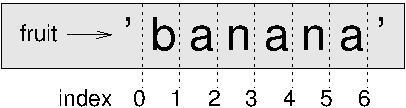
\includegraphics[scale=0.8]{figs/banana.pdf}}
\caption{切片的索引.}
\label{fig.banana}
\end{figure}
%If you omit the first index (before the colon), the slice starts at
%the beginning of the string.  If you omit the second index, the slice
%goes to the end of the string:
如果缺失第一个索引(冒号前), 则切片从字符串头部开始. 
如果忽略了第二个索引, 切片到末尾结束:

\begin{verbatim}
>>> fruit = 'banana'
>>> fruit[:3]
'ban'
>>> fruit[3:]
'ana'
\end{verbatim}
%
%If the first index is greater than or equal to the second the result
%is an {\bf empty string}, represented by two quotation marks:
%\index{quotation mark}
若第一个索引值大于或等于第二个, 则结果为{\bf 空字符串}, 用两个单引号表示:
\index{quotation mark}

\begin{verbatim}
>>> fruit = 'banana'
>>> fruit[3:3]
''
\end{verbatim}
%

%An empty string contains no characters and has length 0, but other
%than that, it is the same as any other string.
空字符串一般不包括任何字符, 同时长度为0, 除此之外, 
和其他字符串一样. 

%Continuing this example, what do you think 
%{\tt fruit[:]} means?  Try it and see.
继续上面的例子, 思考一下{\tt fruit[:]}表示什么? 试试吧. 
\index{copy!slice}
\index{slice!copy}

%\section{Strings are immutable}
\section{字符串不可变}
\index{mutability}
\index{immutability}
\index{string!immutable}


%It is tempting to use the {\tt []} operator on the left side of an
%assignment, with the intention of changing a character in a string.
%For example:
尝试在赋值等式左侧用 {\tt []}操作符修改字符串中的字符. 
例如:
\index{TypeError}
\index{exception!TypeError}

\begin{verbatim}
>>> greeting = 'Hello, world!'
>>> greeting[0] = 'J'
TypeError: 'str' object does not support item assignment
\end{verbatim}
%
%The ``object'' in this case is the string and the ``item'' is
%the character you tried to assign.  For now, an object is
%the same thing as a value, but we will refine that definition
%later (Section~\ref{equivalence}). 
这里的``object''指字符串, ``item''指试图赋值的字符. 
当前, 你可以认为对象和值一样, 但是后续
(在第~\ref{equivalence}节), 我们会对该定义进行细化. 
\index{object}
\index{item}
\index{item assignment}
\index{assignment!item}
\index{immutability}

%The reason for the error is that
%strings are {\bf immutable}, which means you can't change an
%existing string.  The best you can do is create a new string
%that is a variation on the original:
错误的原因在于字符串是{\bf 不可变的}, 
也就是说, 你无法改变一个既有的字符串. 
你能做的, 是基于原来字符串做些操作, 创建一个新的字符串:

\begin{verbatim}
>>> greeting = 'Hello, world!'
>>> new_greeting = 'J' + greeting[1:]
>>> new_greeting
'Jello, world!'
\end{verbatim}
%
%This example concatenates a new first letter onto
%a slice of {\tt greeting}.  It has no effect on
%the original string.
上述代码是用新的首字母和{\tt greeting}的切片进行了拼接, 
而这并不会改变原来的字符串. 
\index{concatenation}

%\section{Searching}
\section{检索}
\label{find}
%What does the following function do?
下面的函数什么用途?
\index{find function}
\index{function!find}

\begin{verbatim}
def find(word, letter):
    index = 0
    while index < len(word):
        if word[index] == letter:
            return index
        index = index + 1
    return -1
\end{verbatim}
%
%In a sense, {\tt find} is the inverse of the {\tt []} operator.
%Instead of taking an index and extracting the corresponding character,
%it takes a character and finds the index where that character
%appears.  If the character is not found, the function returns {\tt
%-1}.
可以认为, {\tt find}是{\tt []}操作符的逆运算. 
此操作不同于根据索引获取对应字符, 
而是根据字符, 查找其索引. 如果字符没有检索到, 
则返回{\tt -1}. 

%This is the first example we have seen of a {\tt return} statement
%inside a loop.  If {\tt word[index] == letter}, the function breaks
%out of the loop and returns immediately.
%
%If the character doesn't appear in the string, the program
%exits the loop normally and  returns {\tt -1}.
%
%This pattern of computation---traversing a sequence and returning
%when we find what we are looking for---is called a {\bf search}.
这是我们第一次见到, 在循环内使用{\tt return}语句. 
如果{\tt word[index] == letter}, 函数会跳出循环, 并立刻返回结果. 

如果字符串中不存在该字符, 程序会一直执行到循环结束, 并
返回{\tt -1}.

这种算法--遍历序列并在找到预期结果时返回--叫做{\bf 检索}. 
\index{traversal}
\index{search pattern}
\index{pattern!search}

%As an exercise, modify {\tt find} so that it has a
%third parameter, the index in {\tt word} where it should start
%looking.
做个练习, 为{\tt find}函数加入第三个参数, 
即在{\tt word}中开始查找的索引位置. 

%\section{Looping and counting}
\section{循环和计数}
\label{counter}
\index{counter}
\index{counting and looping}
\index{looping and counting}
\index{looping!with strings}
%The following program counts the number of times the letter {\tt a}
%appears in a string:
以下程序会统计字符串中{\tt a}出现的次数:

\begin{verbatim}
word = 'banana'
count = 0
for letter in word:
    if letter == 'a':
        count = count + 1
print(count)
\end{verbatim}
%
%This program demonstrates another pattern of computation called a {\bf
%counter}.  The variable {\tt count} is initialized to 0 and then
%incremented each time an {\tt a} is found.
%When the loop exits, {\tt count}
%contains the result---the total number of {\tt a}'s.
此程序描述了另一种算法, 称之为{\bf 计数器}.
初始化变量{\tt count}为0, 其后每找到一次{\tt a}, 就加1.
循环结束后,  {\tt count}便包含了结果-- {\tt a}的全部数量.

\index{encapsulation}
%As an exercise, encapsulate this code in a function named {\tt
%count}, and generalize it so that it accepts the string and the
%letter as arguments.
做个练习, 封装以上代码为{\tt count}函数, 使其以字符串和要计数
的字母为参数, 从而更加通用. 

%Then rewrite the function so that instead of
%traversing the string, it uses the three-parameter version of {\tt
%find} from the previous section.
然后重写该函数, 用上一节的{\tt find}函数的三参数版本, 替换字符串遍历操作. 

%\section{String methods}
\section{字符串方法}
\label{optional}
%Strings provide methods that perform a variety of useful operations.
%A method is similar to a function---it takes arguments and
%returns a value---but the syntax is different.  For example, the
%method {\tt upper} takes a string and returns a new string with
%all uppercase letters.
字符串提供了诸多有用的方法, 方法类似于函数--接受参数
并返回结果--但是语法有些不同. 
例如, {\tt upper}方法, 接收字符串, 
并返回一个全部字母大写后的字符串. 
\index{method}
\index{string!method}

%Instead of the function syntax {\tt upper(word)}, it uses
%the method syntax {\tt word.upper()}.
与函数的语法{\tt upper(word)}不同, 
它使用方法的语法 {\tt word.upper()}.

\begin{verbatim}
>>> word = 'banana'
>>> new_word = word.upper()
>>> new_word
'BANANA'
\end{verbatim}
%
%This form of dot notation specifies the name of the method, {\tt
%upper}, and the name of the string to apply the method to, {\tt
%word}.  The empty parentheses indicate that this method takes no
%arguments.
这种点标法, 声明了方法的名字, {\tt upper}, 
和要使用此方法的字符串的名字, {\tt word}. 
括号为空, 表明此方法未接受任何参数. 
\index{parentheses!empty}
\index{dot notation}

%A method call is called an {\bf invocation}; in this case, we would
%say that we are invoking {\tt upper} on {\tt word}.
方法调用, 通常叫做{\bf 调用};
此例中, 我们会说我们正在对{\tt word}调用{\tt upper}方法. 
\index{invocation}

%As it turns out, there is a string method named {\tt find} that
%is remarkably similar to the function we wrote:
事实证明, 有一个叫{\tt find}的字符串方法, 和我们写的函数
惊人相似:

\begin{verbatim}
>>> word = 'banana'
>>> index = word.find('a')
>>> index
1
\end{verbatim}
%
%In this example, we invoke {\tt find} on {\tt word} and pass
%the letter we are looking for as a parameter.
此例中, 我们调用{\tt word}的{\tt find}方法, 将要查找的字母作为入参. 

%Actually, the {\tt find} method is more general than our function;
%it can find substrings, not just characters:
实际上, {\tt find}方法比我们写的函数要更通用;
它不仅可以定位字符, 也能定位字符串片段:

\begin{verbatim}
>>> word.find('na')
2
\end{verbatim}
%
%By default, {\tt find} starts at the beginning of the string, but
%it can take a second argument, the index where it should start:
默认情况, {\tt find} 从字符串开头开始查找, 不过它也可以接受第二个参数作为索引, 
使其从既定位置开始:
\index{optional argument}
\index{argument!optional}

\begin{verbatim}
>>> word.find('na', 3)
4
\end{verbatim}
%
%This is an example of an {\bf optional argument};
%{\tt find} can
%also take a third argument, the index where it should stop:
这是一个{\bf 可选参数}的例子;
{\tt find}方法也可以接收第三个索引参数, 以标识结束位置:

\begin{verbatim}
>>> name = 'bob'
>>> name.find('b', 1, 2)
-1
\end{verbatim}
%
%This search fails because {\tt b} does not
%appear in the index range from {\tt 1} to {\tt 2}, not including {\tt
%2}.  Searching up to, but not including, the second index makes
%{\tt find} consistent with the slice operator.
因为{\tt b}没有出现在字符串索引{\tt 1}和{\tt 2}且不包括{\tt 2}的范围内, 
所以搜索失败. 
而这种到达第二个索引位但不包括此索引的规则, 和切片操作一样. 

%\section{The {\tt in} operator}
\section{操作符 {\tt in}}
\label{inboth}
\index{in operator}
\index{operator!in}
\index{boolean operator}
\index{operator!boolean}

%The word {\tt in} is a boolean operator that takes two strings and
%returns {\tt True} if the first appears as a substring in the second:
单词 {\tt in}是一个布尔运算符, 其比较两个字符串, 
如果前者是后者的一部分, 
则返回{\tt True}:

\begin{verbatim}
>>> 'a' in 'banana'
True
>>> 'seed' in 'banana'
False
\end{verbatim}
%
%For example, the following function prints all the
%letters from {\tt word1} that also appear in {\tt word2}:
例如, 下面的函数会输出同时出现在{\tt word1}和{\tt word2}中的字母:

\begin{verbatim}
def in_both(word1, word2):
    for letter in word1:
        if letter in word2:
            print(letter)
\end{verbatim}
%

%With well-chosen variable names,
%Python sometimes reads like English.  You could read
%this loop, ``for (each) letter in (the first) word, if (the) letter 
%(appears) in (the second) word, print (the) letter.''
变量名选择得足够好的话, Python读起来便如同英语. 
读一下这个循环, ``for (each) letter in (the first) word, if (the) letter 
(appears) in (the second) word, print (the) letter.''

%Here's what you get if you compare apples and oranges:
下面是apples和oranges比较的结果:

\begin{verbatim}
>>> in_both('apples', 'oranges')
a
e
s
\end{verbatim}
%

%\section{String comparison}
\section{字符串比较}
\index{string!comparison}
\index{comparison!string}

%The relational operators work on strings.  To see if two strings are equal:
关系运算符同样适用于字符串. 
比如要判断两字符串是否相等:

\begin{verbatim}
if word == 'banana':
    print('All right, bananas.')
\end{verbatim}
%
%Other relational operations are useful for putting words in alphabetical
%order:
其他的关系运算符也适用于按照字母顺序进行比较:

\begin{verbatim}
if word < 'banana':
    print('Your word, ' + word + ', comes before banana.')
elif word > 'banana':
    print('Your word, ' + word + ', comes after banana.')
else:
    print('All right, bananas.')
\end{verbatim}
%
%Python does not handle uppercase and lowercase letters the same way
%people do.  All the uppercase letters come before all the
%lowercase letters, so:
Python处理大小写的方式同人类思维不同, 在其看来, 大写字母都排在小写字母之前, 
所以:

\begin{verbatim}
 Pineapple 在前,  banana 在后.
\end{verbatim}
%
%A common way to address this problem is to convert strings to a
%standard format, such as all lowercase, before performing the
%comparison.  Keep that in mind in case you have to defend yourself
%against a man armed with a Pineapple.
解决此问题的常见做法是, 在比较前先统一字符串的格式, 比如都转小写. 
谨记这一点, 以免遇到Pineapple时, 变得一团糟. 


%\section{Debugging}
\section{调试}
\index{debugging}
\index{traversal}

%When you use indices to traverse the values in a sequence,
%it is tricky to get the beginning and end of the traversal
%right.  Here is a function that is supposed to compare two
%words and return {\tt True} if one of the words is the reverse
%of the other, but it contains two errors:
若想用索引来遍历序列中的值, 难点在于确定遍历的起点和终点. 
下面是一个比较单词的函数, 如果一个单词恰好是另一个单词的倒序排列, 
则返回{\tt True}, 但这里有两处错误:

\begin{verbatim}
def is_reverse(word1, word2):
    if len(word1) != len(word2):
        return False
    
    i = 0
    j = len(word2)

    while j > 0:
        if word1[i] != word2[j]:
            return False
        i = i+1
        j = j-1

    return True
\end{verbatim}
%
%The first {\tt if} statement checks whether the words are the
%same length.  If not, we can return {\tt False} immediately.
%Otherwise, for the rest of the function, we can assume that the words
%are the same length.  This is an example of the guardian pattern
%in Section~\ref{guardian}.
第一个 {\tt if} 语句会判断两个单词的长度是否一样. 
如果不同, 立刻返回{\tt False}. 
然而为了执行后续代码, 我们先假设单词长度相同. 
这是一个哨兵模式的示例, 在第~\ref{guardian}节已经介绍过. 
\index{guardian pattern}
\index{pattern!guardian}
\index{index}

%{\tt i} and {\tt j} are indices: {\tt i} traverses {\tt word1}
%forward while {\tt j} traverses {\tt word2} backward.  If we find
%two letters that don't match, we can return {\tt False} immediately.
%If we get through the whole loop and all the letters match, we
%return {\tt True}.
{\tt i} 和 {\tt j}是索引: {\tt i} 正向遍历{\tt word1}, 同时{\tt j} 反向遍历
{\tt word2}. 如果遇到两个字母不同, 则即刻返回{\tt False}. 
如果我们遍历整个循环, 并且所有字母都匹配, 返回{\tt True}. 

%If we test this function with the words ``pots'' and ``stop'', we
%expect the return value {\tt True}, but we get an IndexError:
如果用``pots'' 和 ``stop'' 测试函数, 我们期望得到的是{\tt True}, 
但我们却得到了索引错误:
\index{IndexError}
\index{exception!IndexError}

\begin{verbatim}
>>> is_reverse('pots', 'stop')
...
  File "reverse.py", line 15, in is_reverse
    if word1[i] != word2[j]:
IndexError: string index out of range
\end{verbatim}
%
%For debugging this kind of error, my first move is to
%print the values of the indices immediately before the line
%where the error appears.
调试此种异常, 第一步就是在出现错误的行之前, 先打印索引的值. 

\begin{verbatim}
    while j > 0:
        print(i, j)        # print here
        
        if word1[i] != word2[j]:
            return False
        i = i+1
        j = j-1
\end{verbatim}
%
%Now when I run the program again, I get more information:
现在当我再次运行程序, 获得了更多信息:

\begin{verbatim}
>>> is_reverse('pots', 'stop')
0 4
...
IndexError: string index out of range
\end{verbatim}
%
%The first time through the loop, the value of {\tt j} is 4,
%which is out of range for the string \verb"'pots'".
%The index of the last character is 3, so the
%initial value for {\tt j} should be {\tt len(word2)-1}.
首次循环,  {\tt j} 的值是4,
超出了\verb"'pots'"的索引范围. 
最后一个字符的索引应该是3,
因此{\tt j} 的初始值应该是{\tt len(word2)-1}.


%If I fix that error and run the program again, I get:
如果修复此错误, 并再次执行, 输出如下:

\begin{verbatim}
>>> is_reverse('pots', 'stop')
0 3
1 2
2 1
True
\end{verbatim}
%
%This time we get the right answer, but it looks like the loop only ran
%three times, which is suspicious.  To get a better idea of what is
%happening, it is useful to draw a state diagram.  During the first
%iteration, the frame for \verb"is_reverse" is shown in
%Figure~\ref{fig.state4}.
这次我们的到了正确结果, 但是循环只运行了三次, 有点奇怪. 
为了弄清怎么回事, 可以绘制栈图来辅助理解. 
第一次迭代, \verb"is_reverse"的状态框见图~\ref{fig.state4}.  
\index{state diagram} \index{diagram!state}

\begin{figure}
\centerline
{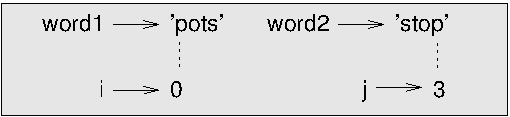
\includegraphics[scale=0.8]{figs/state4.pdf}}
\caption{栈图.}
\label{fig.state4}
\end{figure}

%I took some license by arranging the variables in the frame
%and adding dotted lines to show that the values of {\tt i} and
%{\tt j} indicate characters in {\tt word1} and {\tt word2}.
我尝试在框中排列变量, 并用虚线标识{\tt i} 和
{\tt j}的值, 用来表示在{\tt word1} 和 {\tt word2}中的字符, 
从而帮助理解. 


%Starting with this diagram, run the program on paper, changing the
%values of {\tt i} and {\tt j} during each iteration.  Find and fix the
%second error in this function.
从这个图开始, 尝试在纸上执行程序, 逐次迭代更改{\tt i} 和 {\tt j}值. 
然后找到并修复函数中的第二个错误. 
\label{isreverse}


\section{术语表}
%\section{Glossary}

\begin{description}

%\item[object:] Something a variable can refer to.  For now,
%you can use ``object'' and ``value'' interchangeably.
\item[对象(object):] 变量引用的东西, 目前, 可以将
``对象'' 与 ``值'' 同样看待. 
\index{object}

%\item[sequence:] An ordered collection of
%values where each value is identified by an integer index.
\item[序列(sequence):] 一组有序的值, 每个值由整数索引标识. 
\index{sequence}

%\item[item:] One of the values in a sequence.
\item[元素(item):] 序列中的一个值.
\index{item}

%\item[index:] An integer value used to select an item in
%a sequence, such as a character in a string.  In Python
%indices start from 0.
\item[索引(index):] 一个整数值, 用来选择序列中的元素, 
比如选择字符串中某个字符. 在Python中, 索引都是从0开始. 
\index{index}

%\item[slice:] A part of a string specified by a range of indices.
\item[切片(slice):] 字符串中一部分, 通过索引范围指定. 
\index{slice}

%\item[empty string:] A string with no characters and length 0, represented
%by two quotation marks.
\item[空字符串(empty string):] 不包含任何字符且长度为0的字符串, 用两个引号表示. 
\index{empty string}

%\item[immutable:] The property of a sequence whose items cannot
%be changed.
\item[不可变(immutable):] 序列内元素不可改变的特性. 
\index{immutability}

%\item[traverse:] To iterate through the items in a sequence,
%performing a similar operation on each.
\item[遍历(traverse):] 遍历序列中每个元素, 同时对其执行相似操作的过程. 
\index{traversal}

%\item[search:] A pattern of traversal that stops
%when it finds what it is looking for.
\item[检索(search):] 找到预期目标便停止的一种遍历模式. 
\index{search pattern}
\index{pattern!search}

%\item[counter:] A variable used to count something, usually initialized
%to zero and then incremented.
\item[计数器(counter):] 用来计数的变量, 一般始于0, 不断递增. 
\index{counter}

%\item[invocation:] A statement that calls a method.
\item[调用(invocation):] 调用方法的语句.
\index{invocation}

%\item[optional argument:] A function or method argument that is not
%required.
\item[可选参数(optional argument):] 函数或者方法中的不必要参数. 
\index{optional argument}
\index{argument!optional}

\end{description}


%\section{Exercises}
\section{习题集}

\begin{exercise}
\index{string method}
\index{method!string}

%Read the documentation of the string methods at
%\url{http://docs.python.org/3/library/stdtypes.html#string-methods}.
%You might want to experiment with some of them to make sure you
%understand how they work.  {\tt strip} and {\tt replace} are
%particularly useful.
阅读位于 \url{http://docs.python.org/3/library/stdtypes.html#string-methods}
的文档中的字符串方法, 
可能你会想试试其中一些方法, 尽量弄明白它们的工作原理. 
其中{\tt strip} 和 {\tt replace} 特别有用. 

%The documentation uses a syntax that might be confusing.
%For example, in \verb"find(sub[, start[, end]])", the brackets
%indicate optional arguments.  So {\tt sub} is required, but
%{\tt start} is optional, and if you include {\tt start},
%then {\tt end} is optional.
文档中的某种语法可能难以理解. 
比如\verb"find(sub[, start[, end]])"方法, 方括号标识了可选参数. 
 {\tt sub} 是必需的, 但是{\tt start}是可选的, 
如果包含了 {\tt start}, {\tt end} 便是可选的. 
\index{optional argument}
\index{argument!optional}

\end{exercise}


\begin{exercise}
\index{count method}
\index{method!count}


%There is a string method called {\tt count} that is similar
%to the function in Section~\ref{counter}.  Read the documentation
%of this method
%and write an invocation that counts the number of {\tt a}'s
%in \verb"'banana'".
有个叫{\tt count}的字符串方法, 和第~\ref{counter}节的函数很相似. 
阅读此方法文档, 编写调用此方法的代码, 实现对\verb"'banana'"中
{\tt a}的数量的统计.
\end{exercise}


\begin{exercise}
\index{step size}
\index{slice operator}
\index{operator!slice}

%A string slice can take a third index that specifies the ``step
%size''; that is, the number of spaces between successive characters.
%A step size of 2 means every other character; 3 means every third,
%etc.
字符串切片也可以使用第三个参数, 叫做``步长'';
即相邻字符之间的间隔数. 
步长为2表示每隔一个字符取一个;
步长为3表示每第三个取一个, 依此类推. 

\begin{verbatim}
>>> fruit = 'banana'
>>> fruit[0:5:2]
'bnn'
\end{verbatim}
%A step size of -1 goes through the word backwards, so
%the slice \verb"[::-1]" generates a reversed string.
步长为-1,则表示倒序读取, 所以切片 \verb"[::-1]" , 
便会产生一个反转的字符串. 
\index{palindrome}

%Use this idiom to write a one-line version of \verb"is_palindrome"
%from Exercise~\ref{palindrome}.
用这个神奇的方法, 将习题~\ref{palindrome}中的 \verb"is_palindrome"
修改为一行代码的版本吧. 
\end{exercise}


\begin{exercise}
%The following functions are all {\em intended} to check whether a
%string contains any lowercase letters, but at least some of them are
%wrong.  For each function, describe what the function actually does
%(assuming that the parameter is a string).
下面的函数都是{\em 试图}检验字符串中是否包含小写字母, 
但其中有些函数存在问题. 
仔细分析每个函数并明了其用途
(假设入参都是一个字符串).

\begin{verbatim}
def any_lowercase1(s):
    for c in s:
        if c.islower():
            return True
        else:
            return False

def any_lowercase2(s):
    for c in s:
        if 'c'.islower():
            return 'True'
        else:
            return 'False'

def any_lowercase3(s):
    for c in s:
        flag = c.islower()
    return flag

def any_lowercase4(s):
    flag = False
    for c in s:
        flag = flag or c.islower()
    return flag

def any_lowercase5(s):
    for c in s:
        if not c.islower():
            return False
    return True
\end{verbatim}

\end{exercise}


\begin{exercise}
\index{letter rotation}
\index{rotation, letter}

\label{exrotate}
%A Caesar cypher is a weak form of encryption that involves ``rotating'' each
%letter by a fixed number of places.  To rotate a letter means
%to shift it through the alphabet, wrapping around to the beginning if
%necessary, so 'A' rotated by 3 is 'D' and 'Z' rotated by 1 is 'A'.
凯撒加密(Caesar cypher )是一种通过对每个字母
进行特定数值的``移位''操作, 而实现的弱加密方案. 
对字母移位, 也就是按照字母顺序, 进行移动, 必要时需要回到开头,  
所以'A'移位3, 得到 'D' ,   'Z' 移位1,得到'A'. 

%To rotate a word, rotate each letter by the same amount.
%For example, ``cheer'' rotated by 7 is ``jolly'' and ``melon'' rotated
%by -10 is ``cubed''.  In the movie {\em 2001: A Space Odyssey}, the 
%ship computer is called HAL, which is IBM rotated by -1.
对一个单词移位, 就是对每个字母采用相同的移位数量. 
例如``cheer'' 移位7,则为``jolly'',  ``melon''移位-10, 则为 ``cubed''. 
在电影{\em 2001: A Space Odyssey}中, 飞船上的计算机名叫HAL, 
就是IBM移位-1得到的. 

%For example ``sleep''
%rotated by 9 is ``bunny'' and ``latex'' rotated by 7 is ``shale''.

%Write a function called \verb"rotate_word"
%that takes a string and an integer as parameters, and returns
%a new string that contains the letters from the original string
%rotated by the given amount.  
编写名为\verb"rotate_word"的函数, 接收一个字符串和一个整数, 作为参数, 
对字符串中的字符进行数值移位, 得到新字符串, 并返回. 

%You might want to use the built-in function {\tt ord}, which converts
%a character to a numeric code, and {\tt chr}, which converts numeric
%codes to characters.  Letters of the alphabet are encoded in alphabetical
%order, so for example:
你可能需要用内置的{\tt ord}函数, 此函数可以将字符转为数字码, 
而{\tt chr}则可以将数字码转回字符. 
字母表中的字母会按顺序进行编码, 比如:

\begin{verbatim}
>>> ord('c') - ord('a')
2
\end{verbatim}
%Because \verb"'c'" is the two-eth letter of the alphabet.  But
%beware: the numeric codes for upper case letters are different.
因为\verb"'c'"在字母表中是第2个(从0开始)字母. 
但要注意: 大写字母的数字码和小写的不同. 

%Potentially offensive jokes on the Internet are sometimes encoded in
%ROT13, which is a Caesar cypher with rotation 13.  If you are not
%easily offended, find and decode some of them.  Solution:
%\url{http://thinkpython2.com/code/rotate.py}.
网络上一些冒犯性的笑话有时会采用ROT13编码, 也就是移位数量为13的凯撒加密. 
如果你不会太介意, 试试解密它们吧. 参阅:
\url{http://thinkpython2.com/code/rotate.py}.

\end{exercise}

%\chapter{Case study: word play}
\chapter{案例学习: 单词游戏}
\label{wordplay}

%This chapter presents the second case study, which involves
%solving word puzzles by searching for words that have certain
%properties.  For example, we'll find the longest palindromes
%in English and search for words whose letters appear in
%alphabetical order.  And I will present another program development
%plan: reduction to a previously solved problem.
本章学习第二个案例, 主要研究如何通过搜索特定词汇, 进行猜迷. 
比如, 查找最长回字文, 以及寻找按照字母表顺序排列的单词. 
同时, 我将介绍一种新的程序开发模式: 抽离纷纷扰扰, 回归已有方案. 


\section{读取单词列表}
\label{wordlist}
%For the exercises in this chapter we need a list of English words.
%There are lots of word lists available on the Web, but the one most
%suitable for our purpose is one of the word lists collected and
%contributed to the public domain by Grady Ward as part of the Moby
%lexicon project (see \url{http://wikipedia.org/wiki/Moby_Project}).  It
%is a list of 113,809 official crosswords; that is, words that are
%considered valid in crossword puzzles and other word games.  In the
%Moby collection, the filename is {\tt 113809of.fic}; you can download
%a copy, with the simpler name {\tt words.txt}, from
%\url{http://thinkpython2.com/code/words.txt}.
本章的练习, 需要准备一个英文单词表. 
网上有很多可用的单词表, 但是对我们来说, 最理想的莫过于
Grady Ward 收集整理, 作为Moby词典项目, 贡献给公共领域的单词表
(详见\url{http://wikipedia.org/wiki/Moby_Project}). 这是
包含 113,809 个填词游戏的单词表; 也就是说, 这些单词, 已经在
填词游戏和其他单词游戏中证明了是有效单词. 
在Moby项目中, 这个文件名为 {\tt 113809of.fic};
你可以从\url{http://thinkpython2.com/code/words.txt} 下载一个副本, 
其名字简称 {\tt words.txt}. 
\index{Moby Project}
\index{crosswords}

%This file is in plain text, so you can open it with a text
%editor, but you can also read it from Python.  The built-in
%function {\tt open} takes the name of the file as a parameter
%and returns a {\bf file object} you can use to read the file.
此文件为纯文本文件, 因此你可以用文本编辑器打开, 
但也可以用Python读取. 
内置函数{\tt open}, 以文件名为入参, 返回一个 {\bf 文件对象}, 
你可以用来读取文件内容. 
\index{open function}
\index{function!open}
\index{plain text}
\index{text!plain}
\index{object!file}
\index{file object}

\begin{verbatim}
>>> fin = open('words.txt')
\end{verbatim}
%
%{\tt fin} is a common name for a file object used for input.  The file
%object provides several methods for reading, including {\tt readline},
%which reads characters from the file until it gets to a newline and
%returns the result as a string:
{\tt fin} 是用于输入的文件对象的通用名称. 
文件对象提供了多个读取方法, 包括 {\tt readline}, 
此方法会读取文件的一整行
字符, 并作为字符串返回: 
\index{readline method}
\index{method!readline}

\begin{verbatim}
>>> fin.readline()
'aa\n'
\end{verbatim}
%
%The first word in this particular list is ``aa'', which is a kind of
%lava.  The sequence \verb"\n" represents the newline character that 
%separates this word from the next.
单词列表中第一个单词是``aa'', 这是一种岩浆. 
后面的\verb"\n" 是换行符, 用来断行(将当前单词和后面分隔开). 

%The file object keeps track of where it is in the file, so
%if you call {\tt readline} again, you get the next word:
文件对象会跟踪它在文件的位置(也就是读到了哪里), 从而, 如果再次运行
{\tt readline}, 会得到后面的单词:

\begin{verbatim}
>>> fin.readline()
'aah\n'
\end{verbatim}
%
%The next word is ``aah'', which is a perfectly legitimate
%word, so stop looking at me like that.
%Or, if it's the newline character that's bothering you,
%we can get rid of it with the string method {\tt strip}:
下一个单词是``aah'',  这是个绝对正确的单词, 所以别那样看着我了. 
另外, 如果换行符令你厌烦, 可以用字符串方法{\tt strip}移除:
\index{strip method}
\index{method!strip}

\begin{verbatim}
>>> line = fin.readline()
>>> word = line.strip()
>>> word
'aahed'
\end{verbatim}
%
%You can also use a file object as part of a {\tt for} loop.
%This program reads {\tt words.txt} and prints each word, one
%per line:
你也可以将文件对象置于{\tt for}循环中. 
这样程序便会读取 {\tt words.txt}, 然后逐行输出每个单词:
\index{open function}
\index{function!open}

\begin{verbatim}
fin = open('words.txt')
for line in fin:
    word = line.strip()
    print(word)
\end{verbatim}
%

\section{练习}
%\section{Exercises}
%There are solutions to these exercises in the next section.
%You should at least attempt each one before you read the solutions.
下一节有这些习题的答案, 但在看答案之前最好尽力一试. 

\begin{exercise}
编写程序, 读取{\tt words.txt}, 仅打印多于20个字符的单词
(不包括空格). 
\index{whitespace}

\end{exercise}

\begin{exercise}
%In 1939 Ernest Vincent Wright published a 50,000 word novel called
%{\em Gadsby} that does not contain the letter ``e''.  Since ``e'' is
%the most common letter in English, that's not easy to do.
Ernest Vincent Wright在1939年出版了一部 50,000 单词的小说, 名叫
{\em Gadsby}, 本书不包括字母``e''. 而英文中最常用的便是``e'', 所以
这是很难做到的. 

%In fact, it is difficult to construct a solitary thought without using
%that most common symbol.  It is slow going at first, but with caution
%and hours of training you can gradually gain facility.
事实上, 若不使用常用的字符, 一般很难表达出一个观点. 
不过, 开始虽然进展缓慢, 但是, 通过保持谨慎并训练几个小时, 
你便可以慢慢适应. 

%All right, I'll stop now.
%
%Write a function called \verb"has_no_e" that returns {\tt True} if
%the given word doesn't have the letter ``e'' in it.
好了, 闲言少叙. 

编写 \verb"has_no_e" 函数, 如果输入的单词不包括``e'',  则返回{\tt True}. 

%Write a program that reads {\tt words.txt} and prints only the words
%that have no ``e''.  Compute the percentage of words in the list
%that have no ``e''.
编写程序, 读取{\tt words.txt}, 只打印不包含``e''的单词. 
统计列表中, 不包含``e''的单词所占比例. 
\index{lipogram}

\end{exercise}

\begin{exercise} 

%Write a function named {\tt avoids}
%that takes a word and a string of forbidden letters, and
%that returns {\tt True} if the word doesn't use any of the forbidden
%letters.
编写{\tt avoids}函数, 以单词和一个包含禁用字母的字符串为输入, 
当单词不包含任何禁用字母时, 返回 {\tt True}. 

%Write a program that prompts the user to enter a string
%of forbidden letters and then prints the number of words that
%don't contain any of them.
%Can you find a combination of 5 forbidden letters that
%excludes the smallest number of words?
编写程序, 提示用户输入一个包含禁用字母的字符串, 
然后输出不含有任何禁用字母的单词数量. 
看看你是否可以找出一个包含5个禁用字母的组合, 
使得被排除的单词数最少?

\end{exercise}


\begin{exercise}
%Write a function named \verb"uses_only" that takes a word and a
%string of letters, and that returns {\tt True} if the word contains
%only letters in the list.  Can you make a sentence using only the
%letters {\tt acefhlo}?  Other than ``Hoe alfalfa''?
编写\verb"uses_only"函数 , 以一个单词和一串字母字符串为输入, 
如果单词的字母都在这串字母字符串中, 则返回{\tt True}.
你是否可以只用{\tt acefhlo}这些字母, 构造出句子?
换成 ``Hoe alfalfa''这些字母呢?

\end{exercise}


\begin{exercise} 
%Write a function named \verb"uses_all" that takes a word and a
%string of required letters, and that returns {\tt True} if the word
%uses all the required letters at least once.  How many words are there
%that use all the vowels {\tt aeiou}?  How about {\tt aeiouy}?
编写\verb"uses_all"函数 , 接受一个单词和一串必需字母作为输入, 
如果单词对这些必需字母, 都至少使用了一次, 则返回{\tt True}. 
看看有多少单词同时包含{\tt aeiou}? 又有多少同时包含 {\tt aeiouy}呢?

\end{exercise}


\begin{exercise}
%Write a function called \verb"is_abecedarian" that returns
%{\tt True} if the letters in a word appear in alphabetical order
%(double letters are ok).  
%How many abecedarian words are there?
编写\verb"is_abecedarian"函数, 如果单词中的字母是按照字母表顺序排列, 
则返回 {\tt True}(字母相同, 视为顺序). 看看有多少这种单词?

\index{abecedarian}

\end{exercise}

%\section{Search}
\section{检索}
\label{search}
\index{search pattern}
\index{pattern!search}

%All of the exercises in the previous section have something
%in common; they can be solved with the search pattern we saw
%in Section~\ref{find}.  The simplest example is:
上一章节中, 所有的练习, 都有个共通之处;
它们都可以采用第~\ref{find}节的检索模式来解决. 
举个简单例子:

\begin{verbatim}
def has_no_e(word):
    for letter in word:
        if letter == 'e':
            return False
    return True
\end{verbatim}
%
%The {\tt for} loop traverses the characters in {\tt word}.  If we find
%the letter ``e'', we can immediately return {\tt False}; otherwise we
%have to go to the next letter.  If we exit the loop normally, that
%means we didn't find an ``e'', so we return {\tt True}.
{\tt for}循环会遍历 {\tt word}中所有字母. 
如果遇到 ``e'', 则即刻返回{\tt False};
否则继续查找下一个字母. 
如果循环正常结束, 也就是说没有遇到``e'',  则返回{\tt True}.
\index{traversal}

\index{in operator}
\index{operator!in}
%You could write this function more concisely using the {\tt in}
%operator, but I started with this version because it 
%demonstrates the logic of the search pattern.
你也可以使用{\tt in}运算符来精简程序, 
我先介绍上述版本, 主要是它展示了检索模式的内在逻辑. 

\index{generalization}
%{\tt avoids} is a more general version of \verb"has_no_e" but it
%has the same structure:
{\tt avoids} 函数相比 \verb"has_no_e" 版本, 功能更加通用, 
但结构是相同的:

\begin{verbatim}
def avoids(word, forbidden):
    for letter in word:
        if letter in forbidden:
            return False
    return True
\end{verbatim}
%
%We can return {\tt False} as soon as we find a forbidden letter;
%if we get to the end of the loop, we return {\tt True}.
在此函数中, 一旦遇到禁止字母, 即刻返回{\tt False}, 
如果循环正常结束, 则返回{\tt True}. 

%\verb"uses_only" is similar except that the sense of the condition
%is reversed:
\verb"uses_only" 与之极为相似, 无非条件的含义相反:

\begin{verbatim}
def uses_only(word, available):
    for letter in word: 
        if letter not in available:
            return False
    return True
\end{verbatim}
%
%Instead of a list of forbidden letters, we have a list of available
%letters.  If we find a letter in {\tt word} that is not in
%{\tt available}, we can return {\tt False}.
这里不再是禁用字母列表了, 而是可用字母列表. 
如果在 {\tt word}中找到了不在{\tt available}中的字母, 返回{\tt False}.

%\verb"uses_all" is similar except that we reverse the role
%of the word and the string of letters:
\verb"uses_all"和上述函数也较为相似, 不同之处在于, 
我们颠倒了单词和字母序列的角色:

\begin{verbatim}
def uses_all(word, required):
    for letter in required: 
        if letter not in word:
            return False
    return True
\end{verbatim}
%
%Instead of traversing the letters in {\tt word}, the loop
%traverses the required letters.  If any of the required letters
%do not appear in the word, we can return {\tt False}.
不再是遍历 {\tt word}中的字母, 
而是遍历必需字母列表. 
如果字母列表中有字母未出现在单词中, 返回{\tt False}.
\index{traversal}

%If you were really thinking like a computer scientist, you would
%have recognized that \verb"uses_all" was an instance of a
%previously solved problem, and you would have written:
如若你已像计算机科学家一样去思考, 你便会注意到 \verb"uses_all" 
是以前一个已解决的问题的另一种表达, 你便会这么写:

\begin{verbatim}
def uses_all(word, required):
    return uses_only(required, word)
\end{verbatim}
%
%This is an example of a program development plan called {\bf
%  reduction to a previously solved problem}, which means that you
%recognize the problem you are working on as an instance of a solved
%problem and apply an existing solution. 
此案例便是一个{\bf 抽离纷扰, 回归已知}的程序开发模式的实践, 
这种模式是将遇到的问题, 映射为已解决的问题, 
从而用已有的解决方案来解决当前问题.   
\index{reduction to a previously solved problem} 
\index{development plan!reduction}


%\section{Looping with indices}
\section{索引循环}
\index{looping!with indices}
\index{index!looping with}
%I wrote the functions in the previous section with {\tt for}
%loops because I only needed the characters in the strings; I didn't
%have to do anything with the indices.
前一章节中, 我用{\tt for}循环编写函数, 这是因为我
只需要字符串中的字符; 所以不必理会索引. 

%For \verb"is_abecedarian" we have to compare adjacent letters,
%which is a little tricky with a {\tt for} loop:
但\verb"is_abecedarian"函数中, 我们不得不比较相邻的字母, 
用{\tt for}循环便有些棘手:

\begin{verbatim}
def is_abecedarian(word):
    previous = word[0]
    for c in word:
        if c < previous:
            return False
        previous = c
    return True
\end{verbatim}

%An alternative is to use recursion:
另一种方案是使用递归:

\begin{verbatim}
def is_abecedarian(word):
    if len(word) <= 1:
        return True
    if word[0] > word[1]:
        return False
    return is_abecedarian(word[1:])
\end{verbatim}

%Another option is to use a {\tt while} loop:
还可以使用 {\tt while} 循环:

\begin{verbatim}
def is_abecedarian(word):
    i = 0
    while i < len(word)-1:
        if word[i+1] < word[i]:
            return False
        i = i+1
    return True
\end{verbatim}
%
%The loop starts at {\tt i=0} and ends when {\tt i=len(word)-1}.  Each
%time through the loop, it compares the $i$th character (which you can
%think of as the current character) to the $i+1$th character (which you
%can think of as the next).
此循环始于 {\tt i=0}, 终于{\tt i=len(word)-1}. 
每次循环都会比较第$i$个字符(可以视为当前字符)
和第$i+1$个字符(可以视为下一个字符). 

%If the next character is less than (alphabetically before) the current
%one, then we have discovered a break in the abecedarian trend, and
%we return {\tt False}.
如果下一个字符小于(按字母顺序居前)当前字符, 
我们发现这会破坏顺序递增的趋势, 从而返回{\tt False}.

%If we get to the end of the loop without finding a fault, then the
%word passes the test.  To convince yourself that the loop ends
%correctly, consider an example like \verb"'flossy'".  The
%length of the word is 6, so
%the last time the loop runs is when {\tt i} is 4, which is the
%index of the second-to-last character.  On the last iteration,
%it compares the second-to-last character to the last, which is
%what we want.
如果直到循环结束, 仍然无异常, 则单词通过检验. 
为确信循环正常结束, 可以试试\verb"'flossy'". 
单词长度为6, 所以{\tt i} 为 4时, 便是最后一次循环, 
因为这是倒数第二个字符的索引. 最后一次循环中, 
比较了倒数第二个和倒数第一个字符, 这恰恰符合预期. 
\index{palindrome}

%Here is a version of \verb"is_palindrome" (see
%Exercise~\ref{palindrome}) that uses two indices; one starts at the
%beginning and goes up; the other starts at the end and goes down.
下面是\verb"is_palindrome" 函数(参看习题~\ref{palindrome})的另一个版本, 
其使用了两个索引; 一个从开头到结尾, 顺序前进;
另一个从结尾到开头, 倒序进行.

\begin{verbatim}
def is_palindrome(word):
    i = 0
    j = len(word)-1

    while i<j:
        if word[i] != word[j]:
            return False
        i = i+1
        j = j-1

    return True
\end{verbatim}

%Or we could reduce to a previously solved
%problem and write:
或者, 我们也可以缩减为先前已解决的难题, 写成:
\index{reduction to a previously solved problem}
\index{development plan!reduction}

\begin{verbatim}
def is_palindrome(word):
    return is_reverse(word, word)
\end{verbatim}
%
%Using \verb"is_reverse" from Section~\ref{isreverse}.
此处使用了第~\ref{isreverse}节的\verb"is_reverse"函数.

%\section{Debugging}
\section{调试}
\index{debugging}
\index{testing!is hard}
\index{program testing}

%Testing programs is hard.  The functions in this chapter are
%relatively easy to test because you can check the results by hand.
%Even so, it is somewhere between difficult and impossible to choose a
%set of words that test for all possible errors.
程序测试是很难的. 本章的函数相对容易测试, 
因为你可以用手算来检验结果. 
即便如此, 想要选择一组可以测试所有可能错误的单词, 也是困难重重. 


%Taking \verb"has_no_e" as an example, there are two obvious
%cases to check: words that have an `e' should return {\tt False}, and
%words that don't should return {\tt True}.  You should have no
%trouble coming up with one of each.
以\verb"has_no_e"为例, 有两个明显的情况需要检查: 
一种是含有`e'的单词, 返回{\tt False}, 
另一种是不含有`e'的单词, 返回{\tt True}. 
对此, 你应该可以针对每种情景, 轻松想出一个单词. 

%Within each case, there are some less obvious subcases.  Among the
%words that have an ``e'', you should test words with an ``e'' at the
%beginning, the end, and somewhere in the middle.  You should test long
%words, short words, and very short words, like the empty string.  The
%empty string is an example of a {\bf special case}, which is one of
%the non-obvious cases where errors often lurk.
对于每种情景, 都存在一些不太明显的子用例. 
对于包含 ``e'' 的单词, 你需要检验在单词开头, 结尾, 
以及中间某处带有 ``e'' 的单词. 
你需要检验长单词, 短单词, 甚至非常短的单词, 比如空字符串. 
空字符串是{\bf 特例}的一种, 也就是那种容易被忽视, 
却往往导致错误频发的情况. 
\index{special case}


%In addition to the test cases you generate, you can also test
%your program with a word list like {\tt words.txt}.  By scanning
%the output, you might be able to catch errors, but be careful:
%you might catch one kind of error (words that should not be
%included, but are) and not another (words that should be included,
%but aren't).
除了自己构建测试用例, 你也可以用类似{\tt words.txt}的单词列表检验程序. 
通过扫描输出, 你可能会发现错误, 但要注意: 
你可能发现了一种错误(包括了不应包含的单词), 而忽略了另一种错误
(没有包括应该包含的单词). 

%In general, testing can help you find bugs, but it is not easy to
%generate a good set of test cases, and even if you do, you can't
%be sure your program is correct.
%According to a legendary computer scientist:
通常, 程序测试可以帮助你发现错误, 但要生成好的测试用例, 
往往很难, 即使通过了这些测试, 你也不能百分百地确认你的程序正确. 
一位传奇的计算机科学家说过:
\index{testing!and absence of bugs}

\begin{quote}

%Program testing can be used to show the presence of bugs, but never to
%show their absence!
程序测试只能表明错误的存在, 却永远无法保证其不存在!

--- Edsger W. Dijkstra
\end{quote}
\index{Dijkstra, Edsger}

%\section{Glossary}
\section{术语表}

\begin{description}

%\item[file object:] A value that represents an open file.
\item[文件对象(file object):] 标识一个已打开文件的值.
\index{file object}
\index{object!file}


%\item[reduction to a previously solved problem:] A way of solving a
%  problem by expressing it as an instance of a previously solved
%  problem. 
\item[抽离纷绕, 回归已知(reduction to a previously solved problem):] 一种将当前问题简化为已解决问题, 进而解决问题的方式.
\index{reduction to a previously solved problem}
\index{development plan!reduction}


%\item[special case:] A test case that is atypical or non-obvious
%(and less likely to be handled correctly).
\item[特例(special case):] 非典型或者不明显的测试用例
(往往容易犯错的地方).
\index{special case}

\end{description}

%\section{Exercises}
\section{习题集}

\begin{exercise}
\index{Car Talk}
\index{Puzzler}
\index{double letters}

这个问题源于广播节目 {\em Car Talk} 中的一个迷题
(\url{http://www.cartalk.com/content/puzzlers}):

\begin{quote}
给我一个存在三个连续双字母的单词. 
我会给你一些看似符合, 其实不符的单词. 
例如, 单词committee,  c-o-m-m-i-t-t-e-e. 
如果没有`i' 在中间, 就很完美. 
又或者Mississippi: M-i-s-s-i-s-s-i-p-p-i.
如果将其中的 i 都移除, 便符合了. 
但是有一个词恰好含有三个连续双字母, 而且据我所知, 
这可能是仅有的一个这样的单词. 
当然, 实际上有可能有500多个这样的单词, 但我只能想到一个. 
是哪个单词呢?
\end{quote}

编写程序来寻找一下吧. 
答案: \url{http://thinkpython2.com/code/cartalk1.py}.

\end{exercise}


\begin{exercise}
这也是一个 {\em Car Talk}的迷题(\url{http://www.cartalk.com/content/puzzlers}):
\index{Car Talk}
\index{Puzzler}
\index{odometer}
\index{palindrome}

\begin{quote}

``某天我在高速上开车, 碰巧注意到里程表. 
同多数里程表一样, 它有6个数字, 只能表示整里数. 
所以, 如果我的车跑了300,000英里, 那显示的就是
3-0-0-0-0-0.

``现在, 我看到的很有意思. 最后4个数字是回文;也就是说, 从前往后读
和从后往前读都一样. 比如5-4-4-5 便是个回文, 
所以我的里程表可能显示的是3-1-5-4-4-5.

``一英里后, 最后的5个数字也是回文. 
例如显示为3-6-5-4-5-6. 然后又跑了1英里, 6个数字中间的4位是回文了. 
准备好玩这个了吗?  那又跑了1英里, 所有6个数字也是回文了!

``问题来了, 我开始在里程表上看到的数字是什么?''
\end{quote}

编写个Python程序, 检验所有的6位数字, 然后输出满足上述要求的任意数字. 
答案: \url{http://thinkpython2.com/code/cartalk2.py}.

\end{exercise}


\begin{exercise}
再来一个{\em Car Talk}上的迷题, 你可以用检索法来
解决(\url{http://www.cartalk.com/content/puzzlers}):
\index{Car Talk}
\index{Puzzler}
\index{palindrome}

\begin{quote}
``最近我去看望母亲, 我们发现我的年龄倒过来, 正好是母亲的年龄. 
比如, 若她是73, 我是37. 我们想知道在过去这些年, 有多少次这种情况发生, 
但后来我们岔开了话题, 没有得到答案. 

``回到家后, 我发现到目前为止, 我们的年龄已经互逆了6次. 
同时, 我也意识到, 如果我们幸运的话, 稍后几年, 我们又会年龄互逆一次, 
如果我们特别幸运, 就还会有一次机会. 换句话说, 这样的情况, 可能我们一共会
遇到8次. 所以, 请问, 我现在多少岁了?''

\end{quote}

编写Python程序, 寻找这个迷题的答案. 
提示: 你可能会用到字符串的 {\tt zfill} 方法. 

答案: \url{http://thinkpython2.com/code/cartalk3.py}.

\end{exercise}



\chapter{列表}

本章讲述Python最有用的内置类型, 列表. 
同时你会深入了解对象, 学习一个对象对应多个名称时会产生的现象. 


\section{列表即序列}
\label{sequence}

同字符串一样, {\bf 列表} 也是值的序列. 
字符串中, 值是字符;在列表中, 值可以是任何类型. 
列表中的值, 叫做{\bf 元素}, 有时也叫{\bf 列表项}.
\index{list}
\index{type!list}
\index{element}
\index{sequence}
\index{item}

创建列表的方式很多; 最简单的莫过于将元素用方括号包起来(\verb"[" and \verb"]"):

\begin{verbatim}
[10, 20, 30, 40]
['crunchy frog', 'ram bladder', 'lark vomit']
\end{verbatim}
%
第一个例子是由四个整数构成的列表, 
第二个示例列表则由三个字符串构成. 
列表中的元素类型可以不同. 
下面的列表, 便同时包括了字符串, 浮点数, 整数以及另一个列表:

\begin{verbatim}
['spam', 2.0, 5, [10, 20]]
\end{verbatim}
%
列表中包含列表, 叫做{\bf 嵌套列表}.
\index{nested list}
\index{list!nested}

不包含任何元素的列表, 叫做空列表;
你可以用\verb"[]"创建空列表.
\index{empty list}
\index{list!empty}

如你所想, 列表也可以赋给变量:

\begin{verbatim}
>>> cheeses = ['Cheddar', 'Edam', 'Gouda']
>>> numbers = [42, 123]
>>> empty = []
>>> print(cheeses, numbers, empty)
['Cheddar', 'Edam', 'Gouda'] [42, 123] []
\end{verbatim}
%
\index{assignment}


\section{列表可变}
\label{mutable}
\index{list!element}
\index{access}
\index{index}
\index{bracket operator}
\index{operator!bracket}

从列表中获取元素的语法和从字符串中获取字符的语法一样--方括号操作符. 
括号中的表达式确定了索引值. 
要注意, 索引从0开始:

\begin{verbatim}
>>> cheeses[0]
'Cheddar'
\end{verbatim}
%
和字符串不同, 列表是可变的, 当括号操作符出现在赋值语句左侧, 
就会将对应的列表元素重新赋值. 
\index{mutability}

\begin{verbatim}
>>> numbers = [42, 123]
>>> numbers[1] = 5
>>> numbers
[42, 5]
\end{verbatim}
%
{\tt numbers}中的第一个元素, 原来是123,现在变成了5.
\index{index!starting at zero}
\index{zero, index starting at}


图~\ref{fig.liststate} 是 {\tt cheeses}, {\tt numbers} 和{\tt empty} 的状态图.
\index{state diagram}
\index{diagram!state}

\begin{figure}
\centerline
{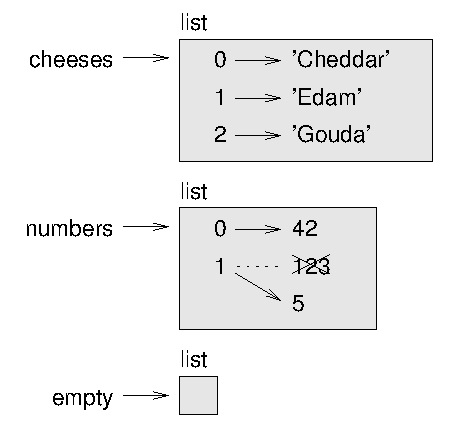
\includegraphics[scale=0.8]{figs/liststate.pdf}}
\caption{状态图.}
\label{fig.liststate}
\end{figure}

列表用单词``list''在外, 元素在内的箱体图表示. 
{\tt cheeses} 指向了一个包括三个元素的列表, 其索引分别为0,1和2. 
{\tt numbers} 包括两个元素; 图中也展现了第二个元素从123 被赋值为5的过程. 
{\tt empty} 指向了一个空列表. 
\index{item assignment}
\index{assignment!item}
\index{reassignment}

列表索引和字符串索引的作用是一样的:

\begin{itemize}

\item 索引可以是任意整型表达式.

\item 如果试图通过索引读写不存在的元素, 会得到{\tt IndexError}.
\index{exception!IndexError}
\index{IndexError}

\item 如果索引为负值, 则从列表末尾倒序计数. 

\end{itemize}
\index{list!index}

\index{list!membership}
\index{membership!list}
\index{in operator}
\index{operator!in}

运算符{\tt in}也可作用于列表. 

\begin{verbatim}
>>> cheeses = ['Cheddar', 'Edam', 'Gouda']
>>> 'Edam' in cheeses
True
>>> 'Brie' in cheeses
False
\end{verbatim}


\section{遍历列表}
\index{list!traversal}
\index{traversal!list}
\index{for loop}
\index{loop!for}
\index{statement!for}

遍历列表中元素的最常用方法便是{\tt for}循环. 语法和字符串遍历相同:

\begin{verbatim}
for cheese in cheeses:
    print(cheese)
\end{verbatim}
%
这种方法对于仅读取列表中元素很方便, 但是如果你想写入或者更新元素, 
那便需要索引了. 
通常把内置函数{\tt range} 和 {\tt len}结合使用:
\index{looping!with indices}
\index{index!looping with}

\begin{verbatim}
for i in range(len(numbers)):
    numbers[i] = numbers[i] * 2
\end{verbatim}
%

此循环会遍历列表并更新每个元素. 
{\tt len}方法会返回列表中元素数量. {\tt range} 则返回从0到 $n-1$的索引值列表, 
其中 $n$ 是列表的长度. 
每次循环, {\tt i}都会获得下一个元素的索引. 循环体中的赋值语句
则会通过{\tt i}获取元素的旧值, 并赋予新值. 
\index{item update}
\index{update!item}

用{\tt for}循环遍历空列表, 永远不会执行循环体:

\begin{verbatim}
for x in []:
    print('This never happens.')
\end{verbatim}
%
虽然列表可以包含其他列表, 但是嵌入的列表仍表示一个元素. 
下面列表的长度为{\tt 4}:
\index{nested list}
\index{list!nested}

\begin{verbatim}
['spam', 1, ['Brie', 'Roquefort', 'Pol le Veq'], [1, 2, 3]]
\end{verbatim}



\section{列表操作}
\index{list!operation}

运算符 {\tt +} 可以用来拼接列表:
\index{concatenation!list}
\index{list!concatenation}

\begin{verbatim}
>>> a = [1, 2, 3]
>>> b = [4, 5, 6]
>>> c = a + b
>>> c
[1, 2, 3, 4, 5, 6]
\end{verbatim}
%

运算符 {\tt *} 会将列表复制给定的次数:
\index{repetition!list}
\index{list!repetition}

\begin{verbatim}
>>> [0] * 4
[0, 0, 0, 0]
>>> [1, 2, 3] * 3
[1, 2, 3, 1, 2, 3, 1, 2, 3]
\end{verbatim}
%
第一个示例复制了{\tt [0]}四次. 
第二个, 则复制了{\tt [1, 2, 3]}三次. 


\section{列表切片}
\index{slice operator}
\index{operator!slice}
\index{index!slice}
\index{list!slice}
\index{slice!list}

切片运算符同样适用于列表:

\begin{verbatim}
>>> t = ['a', 'b', 'c', 'd', 'e', 'f']
>>> t[1:3]
['b', 'c']
>>> t[:4]
['a', 'b', 'c', 'd']
>>> t[3:]
['d', 'e', 'f']
\end{verbatim}
%
如果省略第一位索引, 则从头开始, 进行切片. 
如果省略第二位索引, 则切片止于末尾. 
如果两位都省略, 则切片便等同于复制整个列表. 
\index{list!copy}
\index{slice!copy}
\index{copy!slice}

\begin{verbatim}
>>> t[:]
['a', 'b', 'c', 'd', 'e', 'f']
\end{verbatim}
%
因为列表可变, 所以最好在执行修改列表的操作前, 复制一份, 以防万一. 
\index{mutability}

如果切片运算符在赋值号左侧, 便可以同时更新多个元素:
\index{slice!update}
\index{update!slice}

\begin{verbatim}
>>> t = ['a', 'b', 'c', 'd', 'e', 'f']
>>> t[1:3] = ['x', 'y']
>>> t
['a', 'x', 'y', 'd', 'e', 'f']
\end{verbatim}
%

% 你也可以通过将待更新元素放入空的位置, 从而向列表添加元素
% :

% % \begin{verbatim}
% >>> t = ['a', 'd', 'e', 'f']
% >>> t[1:1] = ['b', 'c']
% >>> print t
% ['a', 'b', 'c', 'd', 'e', 'f']
% \end{verbatim}
% \afterverb
%
% 也可以通过赋值空列表, 从而移除元素. 
% :

% % \begin{verbatim}
% >>> t = ['a', 'b', 'c', 'd', 'e', 'f']
% >>> t[1:3] = []
% >>> print t
% ['a', 'd', 'e', 'f']
% \end{verbatim}
% \afterverb
%
% 但这些操作都可以用更加清晰明了的列表方法替换
% .


\section{列表方法}
\index{list!method}
\index{method, list}

Python 提供了大量操作列表的方法. 例如, 
{\tt append} 可以在列表末尾添加新元素:
\index{append method}
\index{method!append}

\begin{verbatim}
>>> t = ['a', 'b', 'c']
>>> t.append('d')
>>> t
['a', 'b', 'c', 'd']
\end{verbatim}
%
{\tt extend}会以列表为参数, 并将其中所有元素添加到执行列表中:
\index{extend method}
\index{method!extend}

\begin{verbatim}
>>> t1 = ['a', 'b', 'c']
>>> t2 = ['d', 'e']
>>> t1.extend(t2)
>>> t1
['a', 'b', 'c', 'd', 'e']
\end{verbatim}
%
这个例子中, {\tt t2} 没有被修改. 

{\tt sort} 会将列表元素, 从低到高排序:
\index{sort method}
\index{method!sort}

\begin{verbatim}
>>> t = ['d', 'c', 'e', 'b', 'a']
>>> t.sort()
>>> t
['a', 'b', 'c', 'd', 'e']
\end{verbatim}
%
多数列表方法都没有返回值; 这些方法修改列表然后返回{\tt None}. 
如果你意外写了{\tt t = t.sort()}, 结果会令你失望. 
\index{void method}
\index{method!void}
\index{None special value}
\index{special value!None}


\section{Map, filter和reduce}
\label{filter}

若想对列表中所有数字求和, 可以用如下循环实现:

% see add.py

\begin{verbatim}
def add_all(t):
    total = 0
    for x in t:
        total += x
    return total
\end{verbatim}
%
{\tt total}初始为0.
每循环一次{\tt x} 会从列表中获取一个元素. {\tt +=} 操作符, 是一种更新运算的便捷写法. 
也是一种 {\bf 增量赋值语句}. 
\index{update operator}
\index{operator!update}
\index{assignment!augmented}
\index{augmented assignment}

\begin{verbatim}
    total += x
\end{verbatim}
%
等同于

\begin{verbatim}
    total = total + x
\end{verbatim}
%
随着循环运行, {\tt total} 会累积元素求和;
这样的变量有时也称为{\bf 累加器}. 
\index{accumulator!sum}
对列表元素求和, 使用比较普遍, 所以Python提供了内置函数{\tt sum}:

\begin{verbatim}
>>> t = [1, 2, 3]
>>> sum(t)
6
\end{verbatim}
%
像这样将一系列元素合为一个值的操作, 一般称为{\bf reduce}.
\index{reduce pattern}
\index{pattern!reduce}
\index{traversal}

有时, 你会遍历列表, 创建新列表. 例如, 下述函数会接收字符串列表, 
并返回一个将所有字符串都转为首字母大写的字符串列表:

\begin{verbatim}
def capitalize_all(t):
    res = []
    for s in t:
        res.append(s.capitalize())
    return res
\end{verbatim}
%
{\tt res} 开始是一个空列表; 每次循环, 都会向其中添加下一个元素. 
所以{\tt res}也可认为是另一种累加器. 
\index{accumulator!list}

类似\verb"capitalize_all"这样的操作, 一般叫做{\bf map}, 
因为此操作会将函数(此处为{\tt capitalize})``应用''到序列中每个元素上. 
\index{map pattern}
\index{pattern!map}
\index{filter pattern}
\index{pattern!filter}

另一种常用操作是, 从列表中筛选部分元素, 返回子列表. 例如, 
下面函数会接收一个字符串列表, 返回仅包含大写字母的字符串列表:

\begin{verbatim}
def only_upper(t):
    res = []
    for s in t:
        if s.isupper():
            res.append(s)
    return res
\end{verbatim}
%
{\tt isupper}是字符串方法, 如果字符串中字母全部为大写, 则返回{\tt True}. 

如\verb"only_upper" 一样的操作, 叫做 {\bf filter}, 因为此操作会筛选出某些元素, 
过滤掉其他元素. 

大部分的列表操作都可以由map, filter 以及reduce 组合构成. 


\section{移除元素}
\index{element deletion}
\index{deletion, element of list}

从列表中移除元素有多种方法. 
如果你知道所要移除元素的索引, 可以用
{\tt pop}方法:
\index{pop method}
\index{method!pop}

\begin{verbatim}
>>> t = ['a', 'b', 'c']
>>> x = t.pop(1)
>>> t
['a', 'c']
>>> x
'b'
\end{verbatim}
%
{\tt pop} 会改变列表, 并返回被移除的元素. 
如果未提供索引, 则会删除并返回最后一个元素. 

如果你不使用移除的元素, 则可以用{\tt del}元算符:
\index{del operator}
\index{operator!del}

\begin{verbatim}
>>> t = ['a', 'b', 'c']
>>> del t[1]
>>> t
['a', 'c']
\end{verbatim}
%
如果你知道要删除元素的值(但不知道索引位置), 你可以用{\tt remove}方法:
\index{remove method}
\index{method!remove}

\begin{verbatim}
>>> t = ['a', 'b', 'c']
>>> t.remove('b')
>>> t
['a', 'c']
\end{verbatim}
%
{\tt remove} 方法的返回值是{\tt None}.
\index{None special value}
\index{special value!None}

如果要移除多个元素, 可以用 {\tt del}配合切片索引实现:

\begin{verbatim}
>>> t = ['a', 'b', 'c', 'd', 'e', 'f']
>>> del t[1:5]
>>> t
['a', 'f']
\end{verbatim}
%
通常, 切片含头不含尾, 即到第二个索引值(不包括)为止. 



\section{列表和字符串}
\index{list}
\index{string}
\index{sequence}

字符串是一系列的字符, 列表是一系列的值, 但是字符列表和字符串并不可等同视之. 
采用 {\tt list}方法, 可以将字符串转换为字符列表:
\index{list!function}
\index{function!list}

\begin{verbatim}
>>> s = 'spam'
>>> t = list(s)
>>> t
['s', 'p', 'a', 'm']
\end{verbatim}
%
因{\tt list}是一个内置函数的名字, 所以尽量避免将其作为变量名. 
我通常也不建议使用{\tt l} , 因为和{\tt 1}太像了. 这便是我用
{\tt t}作为变量名的缘由. 

{\tt list}函数可以将字符串拆解为单独的字母. 
如果你想将字符串分拆为一个个单词, 则可以使用{\tt split}方法:
\index{split method}
\index{method!split}

\begin{verbatim}
>>> s = 'pining for the fjords'
>>> t = s.split()
>>> t
['pining', 'for', 'the', 'fjords']
\end{verbatim}
%
此处的可选参数是{\bf 分隔符}, 也就是定义单词边界的字符. 
下面的示例使用连字符作为分隔符:
\index{optional argument}
\index{argument!optional}
\index{delimiter}

\begin{verbatim}
>>> s = 'spam-spam-spam'
>>> delimiter = '-'
>>> t = s.split(delimiter)
>>> t
['spam', 'spam', 'spam']
\end{verbatim}
%
{\tt join}和 {\tt split}的作用正好相反. 
它会接收字符串列表, 然后拼接所有元素. 
{\tt join}是一个字符串方法, 所以你需要
在分隔符上调用此方法, 然后将列表作为参数传入:
\index{join method}
\index{method!join}
\index{concatenation}

\begin{verbatim}
>>> t = ['pining', 'for', 'the', 'fjords']
>>> delimiter = ' '
>>> s = delimiter.join(t)
>>> s
'pining for the fjords'
\end{verbatim}
%
此例中, 分隔符是一个空格, 
{\tt join}会在每个单词之间放置一个空格. 
若想不用空格拼接, 则可以用空字符串\verb"''"作为分隔符. 
\index{empty string}
\index{string!empty}


\section{对象和值}
\label{equivalence}
\index{object}
\index{value}

如果运行下面的赋值语句:

\begin{verbatim}
a = 'banana'
b = 'banana'
\end{verbatim}
%
我们知道{\tt a} 和 {\tt b}都指向了字符串, 但我们不知道, 他们是否指向
了{\em 相同的} 字符串. 
所以, 便有了两种可能状态, 如图~\ref{fig.list1}.
\index{aliasing}

\begin{figure}
\centerline
{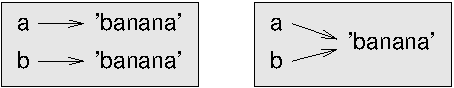
\includegraphics[scale=0.8]{figs/list1.pdf}}
\caption{状态图.}
\label{fig.list1}
\end{figure}

第一种情况, {\tt a} 和 {\tt b}指向了两个不同对象, 这两个对象
有相同的值. 第二种情况, 它们指向了同一个对象. 
\index{is operator}
\index{operator!is}

若想判断两个变量是否指向了同一个对象, 可以用{\tt is}运算符.

\begin{verbatim}
>>> a = 'banana'
>>> b = 'banana'
>>> a is b
True
\end{verbatim}
%
此例中, Python仅创建了一个字符串对象, 然后{\tt a} 
和 {\tt b} 都指向了此对象. 
但是当你创建两个列表时, 你得到的就是两个对象:

\begin{verbatim}
>>> a = [1, 2, 3]
>>> b = [1, 2, 3]
>>> a is b
False
\end{verbatim}
%

此时, 状态图便是图~\ref{fig.list2}的样子.
\index{state diagram}
\index{diagram!state}

\begin{figure}
\centerline
{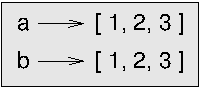
\includegraphics[scale=0.8]{figs/list2.pdf}}
\caption{状态图.}
\label{fig.list2}
\end{figure}

这种情况下, 可以说这两个列表是{\bf 相等的},
因为它们有相同的元素, 
但它们不是{\bf 相同的}, 因为不是同一个对象. 
两个对象如果相同, 那么它们必然相等, 
但是它们如果相等, 却未必相同. 
\index{equivalence}
\index{identity}

到目前为止, 我们一直混用``对象''和 ``值'', 但更准确地说, 
一个对象有一个值. 若创建{\tt [1, 2, 3]}, 你会得到一个列表对象, 
而这个对象的值是个整数序列. 
如果另外一个列表也有相同的元素, 我们便说它们拥有相同的值, 
但它们不是同一个对象. 
\index{object}
\index{value}


\section{别称}
\index{aliasing}
\index{reference!aliasing}

如果 {\tt a} 指向一个对象, 同时令{\tt b = a},
那么, 两个变量都指向了同一个对象:

\begin{verbatim}
>>> a = [1, 2, 3]
>>> b = a
>>> b is a
True
\end{verbatim}
%
此时状态图如图~\ref{fig.list3}所示.
\index{state diagram}
\index{diagram!state}

\begin{figure}
\centerline
{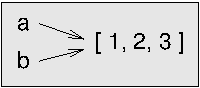
\includegraphics[scale=0.8]{figs/list3.pdf}}
\caption{状态图.}
\label{fig.list3}
\end{figure}

变量和对象的这种关联, 叫做{\bf 引用}.
上例中, 两个引用指向了同一个对象. 
\index{reference}

有多个引用的对象, 也便有了多个名称, 
如此, 我们可以说, 对象是有{\bf 别称的}.
\index{mutability}

如果一个有别称的对象是可变的, 那么一个别称所做的修改会影响另一个:

\begin{verbatim}
>>> b[0] = 42
>>> a
[42, 2, 3]
\end{verbatim}
%

虽然此特性很有用, 但也很容易出错. 
通常, 对于可变对象, 避免使用别称, 会安全很多. 
\index{immutability}

而对于像字符串这样的不可变对象, 别称使用往往不是问题. 
如下所示:

\begin{verbatim}
a = 'banana'
b = 'banana'
\end{verbatim}
%
所以{\tt a} 和 {\tt b} 是否指向同一个对象, 已无关紧要. 


\section{列表参数}
\label{list.arguments}
\index{list!as argument}
\index{argument}
\index{argument!list}
\index{reference}
\index{parameter}

当给函数传递列表时, 函数收到的是对该列表的引用. 
如果函数修改了列表, 那么调用一方也会看到相应变化. 
例如, \verb"delete_head" 函数删除了列表中第一个元素:

\begin{verbatim}
def delete_head(t):
    del t[0]
\end{verbatim}
%

下面是一个应用:

\begin{verbatim}
>>> letters = ['a', 'b', 'c']
>>> delete_head(letters)
>>> letters
['b', 'c']
\end{verbatim}
%
形参{\tt t}和变量{\tt letters}是同一个变量的别称. 
栈图如图~\ref{fig.stack5}所示.
\index{stack diagram}
\index{diagram!stack}

\begin{figure}
\centerline
{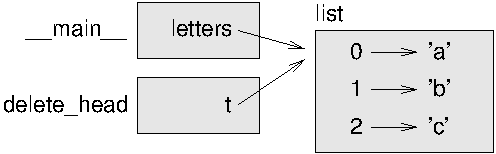
\includegraphics[scale=0.8]{figs/stack5.pdf}}
\caption{栈图.}
\label{fig.stack5}
\end{figure}

因两个框共用一个列表, 所以我把列表画在了它们中间. 

区分修改列表操作和新建列表操作, 是非常重要的. 
例如,  {\tt append}方法是修改列表, 而{\tt +}运算符则会新建列表.
\index{append method}
\index{method!append}
\index{list!concatenation}
\index{concatenation!list}

下面是{\tt append}的一个使用示例:
%
\begin{verbatim}
>>> t1 = [1, 2]
>>> t2 = t1.append(3)
>>> t1
[1, 2, 3]
>>> t2
None
\end{verbatim}
%
{\tt append} 的返回值是 {\tt None}.

下面是使用 {\tt +}运算符的示例:
%
\begin{verbatim}
>>> t3 = t1 + [4]
>>> t1
[1, 2, 3]
>>> t3
[1, 2, 3, 4]
\end{verbatim}
%
操作结果是个新列表, 原列表也没有变化.

在为修改列表而编写函数时, 此差异尤要重视. 
例如, 下面函数{\em 没有}删除列表的第一个元素:
%
\begin{verbatim}
def bad_delete_head(t):
    t = t[1:]              # WRONG!
\end{verbatim}
%
此切片运算符会新建列表, 同时赋值号令 {\tt t}指向此新列表, 
但是这个操作并不会影响调用者.
\index{slice operator}
\index{operator!slice}
%
\begin{verbatim}
>>> t4 = [1, 2, 3]
>>> bad_delete_head(t4)
>>> t4
[1, 2, 3]
\end{verbatim}
%

\verb"bad_delete_head"函数开始运行时, {\tt t} 和 {\tt t4} 指向了同一个
列表. 函数结束时, {\tt t}指向了新的列表, 
但是{\tt t4} 仍然指向了原来的,未被修改的列表.

一种替代方案是, 编写一个创建并返回新列表的函数. 比如, 
{\tt tail}函数会返回列表中除首元素的所有元素列表:

\begin{verbatim}
def tail(t):
    return t[1:]
\end{verbatim}
%
此函数依然会保持原列表不变. 下面是用法:

\begin{verbatim}
>>> letters = ['a', 'b', 'c']
>>> rest = tail(letters)
>>> rest
['b', 'c']
\end{verbatim}



\section{调试}
\index{debugging}

若使用列表(和其他可变对象)时不够小心谨慎, 很容易导致长达数小时的调试跟踪. 
这里有一些常见陷阱以及如何避免:

\begin{enumerate}

\item 多数的列表方法都是传入参数, 返回 {\tt None}. 
这和字符串方法恰恰相反, 字符串方法一般返回新字符串, 
同时保持原始值不变. 

如果你惯于编写下面这样的代码:

\begin{verbatim}
word = word.strip()
\end{verbatim}

那么你可能会写出下面这样的代码:

\begin{verbatim}
t = t.sort()           # WRONG!
\end{verbatim}
\index{sort method}
\index{method!sort}

因为 {\tt sort}返回的是{\tt None}, 所以后续对{\tt t}的操作多会失败.

在使用列表方法前, 你应该认真阅读文档, 并在交互模式下测试一下. 

\item 确定原则, 坚定执行.

列表使用中面临的部分问题在于, 有多条道路通罗马. 
比如, 从列表中移除元素, 你可以用 {\tt pop}, {\tt remove}, {\tt del},
甚至用切片重新赋值. 

若想给列表添加元素, 可以用{\tt append}方法, 或者{\tt +}运算符. 
假设{\tt t}是列表, {\tt x}是列表元素, 下面的操作都正确: 

\begin{verbatim}
t.append(x)
t = t + [x]
t += [x]
\end{verbatim}

而下面的代码是错误的:

\begin{verbatim}
t.append([x])          # WRONG!
t = t.append(x)        # WRONG!
t + [x]                # WRONG!
t = t + x              # WRONG!
\end{verbatim}

在交互模式下测试每个示例, 确保理解其作用. 
你会注意到, 只有最后一个会报运行时异常;
其他三个语句合法, 但并不会得到想要的效果. 


\item 复制列表, 避免别称.
\index{aliasing!copying to avoid}
\index{copy!to avoid aliasing}

你若想使用{\tt sort} 方法修改参数, 同时又想保留原列表, 那你可以复制一份. 

\begin{verbatim}
>>> t = [3, 1, 2]
>>> t2 = t[:]
>>> t2.sort()
>>> t
[3, 1, 2]
>>> t2
[1, 2, 3]
\end{verbatim}

此例中, 你也可以使用内置函数{\tt sorted}, 
此函数可以返回新的排好序的列表, 同时又保留了原始列表. 
\index{sorted!function}
\index{function!sorted}

\begin{verbatim}
>>> t2 = sorted(t)
>>> t
[3, 1, 2]
>>> t2
[1, 2, 3]
\end{verbatim}

\end{enumerate}



\section{术语表}

\begin{description}

\item[列表(list):] 由值构成的序列. 
\index{list}

\item[元素(element):] 列表(或序列)中的值, 也可以称为列表项.
\index{element}

\item[嵌套列表(nested list):] 列表中的元素是另外的列表. 
\index{nested list}

\item[累加器(accumulator):] 在循环中用于累加或累积结果的变量.
\index{accumulator}

\item[增强赋值(augmented assignment):] 使用 \verb"+=" 这样的操作符更新变量值的
赋值语句.
\index{assignment!augmented}
\index{augmented assignment}
\index{traversal}

\item[reduce:] 一种遍历序列, 并累加元素为一个元素的处理模式.
\index{reduce pattern}
\index{pattern!reduce}

\item[map:] 一种遍历序列, 对每个元素都执行同一操作的处理模式.
\index{map pattern}
\index{pattern!map}

\item[filter:] 一种遍历列表, 并筛选满足特定条件的元素的处理模式.
\index{filter pattern}
\index{pattern!filter}

\item[对象(object):] 变量之指向. 对象拥有特定类型以及值.
\index{object}

\item[相等(equivalent):] 拥有相同的值.
\index{equivalent}

\item[相同(identical):] 指向同一个对象(也就意味着相等).
\index{identical}

\item[引用(reference):] 变量和其指向的值之间的关系.
\index{reference}

\item[别称(aliasing):] 多个变量指向同一个对象的情况.
\index{aliasing}

\item[分隔符(delimiter):] 用来界定长字符串分隔位置的字符和字符串.
\index{delimiter}

\end{description}


\section{习题集}

大家可以从\url{http://thinkpython2.com/code/list_exercises.py}
下载这些习题的答案.

\begin{exercise}

编写 \verb"nested_sum" 函数, 接收包含整数列表的一个列表, 
然后将所有内嵌列表的元素相加求和. 
比如:

\begin{verbatim}
>>> t = [[1, 2], [3], [4, 5, 6]]
>>> nested_sum(t)
21
\end{verbatim}

\end{exercise}

\begin{exercise}
\label{cumulative}
\index{cumulative sum}
编写函数{\tt cumsum} , 使其接收一个数字列表, 返回累加之和;
也就是, 第$i$个元素是原列表中的第$i+1$个元素之前所有元素之和. 
比如:

\begin{verbatim}
>>> t = [1, 2, 3]
>>> cumsum(t)
[1, 3, 6]
\end{verbatim}

\end{exercise}

\begin{exercise}

编写\verb"middle"函数, 接收一个列表, 返回包含掐头去尾后所有元素的新列表. 
比如:

\begin{verbatim}
>>> t = [1, 2, 3, 4]
>>> middle(t)
[2, 3]
\end{verbatim}

\end{exercise}

\begin{exercise}
编写函数 \verb"chop" , 使其接收一个列表, 然后移除首尾元素, 返回 {\tt None}.
例如:

\begin{verbatim}
>>> t = [1, 2, 3, 4]
>>> chop(t)
>>> t
[2, 3]
\end{verbatim}

\end{exercise}


\begin{exercise}
编写 \verb"is_sorted"函数, 接收一个列表, 如果列表是升序排列, 则返回 {\tt True}, 
否则返回 {\tt False}. 例如:

\begin{verbatim}
>>> is_sorted([1, 2, 2])
True
>>> is_sorted(['b', 'a'])
False
\end{verbatim}

\end{exercise}


\begin{exercise}
\label{anagram}
\index{anagram}

如果一个单词, 通过重新排列字母, 得到另一单词, 则称两个词为字母异位词. 
编写\verb"is_anagram"函数, 接收两个字符串, 如果两者为字母异位词, 返回{\tt True}.
\end{exercise}



\begin{exercise}
\label{duplicate}
\index{duplicate}
\index{uniqueness}

编写\verb"has_duplicates" 函数, 使其接收一个列表, 如果列表中
存在重复出现的元素, 返回{\tt True}. 注意不要修改原始列表.

\end{exercise}


\begin{exercise}

此题属于生日悖论, 你可以参考\url{http://en.wikipedia.org/wiki/Birthday_paradox}
了解更多.
\index{birthday paradox}

如果你的班上有23名学生, 那其中两人的生日相同的概率是多少? 
你可以生成23个随机的生日样本, 检查其是否存在相同, 从而估计概率值. 
提示: 你可以通过{\tt random}模块中的{\tt randint} 函数来制造随机生日. 
\index{random module}
\index{module!random}
\index{randint function}
\index{function!randint}

可以从 \url{http://thinkpython2.com/code/birthday.py} 下载我的代码.

\end{exercise}


\begin{exercise}
\index{append method}
\index{method!append}
\index{list!concatenation}
\index{concatenation!list}

编写函数读取{\tt words.txt} 内容, 并将其中每个单词放入列表中. 
写两个版本, 一个采用{\tt append}方法, 另一个则用 {\tt t = t + [x]} 实现. 
哪种耗时较长? 为什么?

代码参见: \url{http://thinkpython2.com/code/wordlist.py}.
\index{time module}
\index{module!time}

\end{exercise}


\begin{exercise}
\label{wordlist1}
\label{bisection}
\index{membership!bisection search}
\index{bisection search}
\index{search, bisection}
\index{membership!binary search}
\index{binary search}
\index{search, binary}
若要检验一个单词是否在列表中, 可以用{\tt in}运算符, 
但是速度会慢, 因为它是从头开始, 顺序检索. 

由于这些单词通常是按照字母表顺序排列, 我们可以通过对折查找
(也叫二分查找), 提高速度. 此方法和你通过字典(此处指书籍, 不是数据结构)
查找单词的方式很像. 
你一般会先翻到字典中间, 然后看单词在之前, 还是之后. 如果在前面, 则继续此
方法查找, 如果在后面, 同样操作. 

无论怎样, 你都可以将搜索区间减半. 
如果单词列表有113,809 个单词, 大约17次, 你就可以定位到单词, 
或者确定其不在其中.

编写函数\verb"in_bisect",  使其接收一个有序列表, 以及一个目标值, 
当单词在列表中时, 返回{\tt True},  否则返回{\tt False}. 
\index{bisect module}
\index{module!bisect}

你也可以阅读{\tt bisect}模块相关文档, 进而使用它!
可以参看代码: \url{http://thinkpython2.com/code/inlist.py}.

\end{exercise}

\begin{exercise}
\index{reverse word pair}

如果两个单词拼写顺序相反, 则称其为``逆序对''.
编写程序, 查找单词列表中所有逆序对.
参见代码: \url{http://thinkpython2.com/code/reverse_pair.py}.

\end{exercise}

\begin{exercise}
\index{interlocking words}
如果从两个单词交替获取字母, 构成新单词, 便称其``连锁''. 
比如 ``shoe'' 和``cold'', 交替获取字母, 构成了``schooled''. 
答案见: \url{http://thinkpython2.com/code/interlock.py}.
致谢: 此习题源于 \url{http://puzzlers.org} 的一个例子.

\begin{enumerate}

\item 编写函数, 寻找所有连锁单词对. 提示:不要枚举所有单词对!

\item 你能找到三路连锁的单词吗; 也就是从三个单词, 第一个, 第二个, 第三个, 
每次获取三个字母, 从而构成新单词?

\end{enumerate}
\end{exercise}


\chapter{字典}

本章讲述另一个内置类型, 字典. 
字典是Python最优秀的特性之一; 同时也是诸多高效且优雅算法的基石. 


\section{字典即映射}

\index{dictionary}
\index{dictionary}
\index{type!dict}
\index{key}
\index{key-value pair}
\index{index}

 {\bf 字典} 如同列表, 但更加通用. 列表中, 索引必须是整数, 
而在字典中, 索引(几乎)可以是任何类型. 

字典包括一个索引集合, 叫做{\bf 键(keys)}, 以及一个值的集合. 
每个键都和一个值相关联. 键和值的这种对应关系, 叫做{\bf 键值对(key-value pair)}
或者叫做 {\bf 项(item)}.  \index{item}

数学语言中, 字典代表了从键到值的{\bf 映射(mapping)}关系, 
所以你也可以说, 每个键都``映射''了一个值. 
举个例子, 我们构建个字典, 使其将英语单词映射到西班牙语单词, 
那么, 键和值便都是字符串. 

函数{\tt dict}用来创建一个新的空字典. 
由于{\tt dict}是内置函数名, 你要尽量避免将其用作变量名. 
\index{dict function}
\index{function!dict}

\begin{verbatim}
>>> eng2sp = dict()
>>> eng2sp
{}
\end{verbatim}

花括号 \verb"{}", 表示一个空字典. 
要想向其中添加项, 可以用方括号:
\index{squiggly bracket}
\index{bracket!squiggly}

\begin{verbatim}
>>> eng2sp['one'] = 'uno'
\end{verbatim}
%
这行代码创建了一个从键\verb"'one'"到值\verb"'uno'"的映射的项. 
如果你再次打印字典, 可以看到一个键值对, 其键和值用冒号隔开:

\begin{verbatim}
>>> eng2sp
{'one': 'uno'}
\end{verbatim}
%

这种输出格式也可以是输入的格式. 比如, 用三个项创建一个新字典:

\begin{verbatim}
>>> eng2sp = {'one': 'uno', 'two': 'dos', 'three': 'tres'}
\end{verbatim}
%
但你打印{\tt eng2sp}, 会感到意外:

\begin{verbatim}
>>> eng2sp
{'one': 'uno', 'three': 'tres', 'two': 'dos'}
\end{verbatim}
%
键值对的顺序不一样了. 
如果你在电脑输入上述代码, 可能结果也不一样. 
通常, 字典中项的顺序是很难确定的. 

但是这往往不是个问题, 因为字典的元素从来不是用整数索引去检索的. 
而是用键来寻找相应的值:

\begin{verbatim}
>>> eng2sp['two']
'dos'
\end{verbatim}
%
键\verb"'two'"总是映射到值\verb"'dos'" , 所以项的顺序就无关紧要了. 

如果键不在字典中, 你会得到异常:
\index{exception!KeyError}
\index{KeyError}

\begin{verbatim}
>>> eng2sp['four']
KeyError: 'four'
\end{verbatim}
%
 {\tt len} 函数对于字典同样有效; 它会返回键-值对的数量:
\index{len function}
\index{function!len}

\begin{verbatim}
>>> len(eng2sp)
3
\end{verbatim}
%
运算符{\tt in}对字典也同样有效;
它可以判断某个{\em key} 是否存在于字典的键中(而不是值中). 
\index{membership!dictionary}
\index{in operator}
\index{operator!in}

\begin{verbatim}
>>> 'one' in eng2sp
True
>>> 'uno' in eng2sp
False
\end{verbatim}
%
若要确定值是否存在于字典中, 可以用{\tt values}方法, 它会返回值的集合,  
然后使用{\tt in}运算符:
\index{values method}
\index{method!values}

\begin{verbatim}
>>> vals = eng2sp.values()
>>> 'uno' in vals
True
\end{verbatim}
%
运算符{\tt in}在列表和字典中使用的算法不同. 
对于列表来说, 它会如第~\ref{find}节一样, 按照顺序搜索列表中的元素. 
随着列表变长, 确定目标的耗时也会更长. 

Python中的字典则使用了叫做{\bf 哈希表}的数据结构, 使其具有了一个神奇特性: 
无论字典中有多少项, {\tt in} 运算符都耗时相同. 
我会在第~\ref{hashtable}节解释其原理, 暂时这些还不重要. 

\section{以字典为计数器}
\label{histogram}
\index{counter}

假设有个字符串, 你需要统计每个字母出现的次数. 
有多种方法可以实现:

\begin{enumerate}

\item 你可以新建26个变量, 对应字母表中的每个字母. 
然后遍历字符串, 遇到哪个字母, 相应计数器就加一, 
可能会用到链式条件. 

\item 你也可以创建一个包含26个元素的列表. 
把每个字母转换成数字(使用内置函数{\tt ord}), 用这些数字作为列表的索引, 
然后累加相应计数器. 

\item 你也可以新建一个字典, 这个字典将字母作为键, 
将计数器作为相应的值. 
字母首次出现, 便在字典中添加一个项, 后面再出现, 便可以对
已有的项累加即可. 

\end{enumerate}

上述各个方案, 目标相同, 手段各异.
\index{implementation}

一种{\bf 实现}便是一种运算方式; 有好有坏. 
比如, 用字典实现的优势在于, 我们无需提前知道字符串中存在哪些字母, 
我们只需要为每个出现的字母提供空间而已. 

下面是代码实现:

\begin{verbatim}
def histogram(s):
    d = dict()
    for c in s:
        if c not in d:
            d[c] = 1
        else:
            d[c] += 1
    return d
\end{verbatim}
%
这个函数名是 {\tt histogram(直方图)}, 是个统计术语, 表示计数(或者频次)的集合.
\index{histogram}
\index{frequency}
\index{traversal}

函数第一行新建了一个空字典. 
然后用 {\tt for} 循环遍历字符串. 每次循环中, 如果字符{\tt c}不在字典中, 
则创建一个新的项, 将{\tt c}作键, 初始值为1(只遇到了一次). 
如果{\tt c} 已经在字典中, 则 {\tt d[c]}加一.
\index{histogram}

下面为执行样例:

\begin{verbatim}
>>> h = histogram('brontosaurus')
>>> h
{'a': 1, 'b': 1, 'o': 2, 'n': 1, 's': 2, 'r': 2, 'u': 2, 't': 1}
\end{verbatim}
%

结果表明字母 \verb"'a'"和 \verb"'b'"只出现了一次;
\verb"'o'"出现了两次, 等等. 


\index{get 方法}
\index{method!get}
字典有个方法, 叫做{\tt get}, 
以键和默认值为参数. 
如果键在字典中, {\tt get} 则返回对应的值;否则, 会返回默认值. 
如下:

\begin{verbatim}
>>> h = histogram('a')
>>> h
{'a': 1}
>>> h.get('a', 0)
1
>>> h.get('c', 0)
0
\end{verbatim}
%
做个练习, 用{\tt get} 来精炼一下{\tt histogram}函数. 
尽量避免使用{\tt if}语句. 

\section{循环和字典}
\index{dictionary!looping with}
\index{looping!with dictionaries}
\index{traversal}

如果你针对字典应用{\tt for}语句, 它会遍历所有的键. 
比如, \verb"print_hist"函数会输出每个键以及其相应的值:

\begin{verbatim}
def print_hist(h):
    for c in h:
        print(c, h[c])
\end{verbatim}
%
下面为输出结果:

\begin{verbatim}
>>> h = histogram('parrot')
>>> print_hist(h)
a 1
p 1
r 2
t 1
o 1
\end{verbatim}
%
又是这样, 这些键没有按照顺序输出. 
若要按顺序遍历键, 可以用内置函数{\tt sorted}:
\index{sorted!function}
\index{function!sorted}

\begin{verbatim}
>>> for key in sorted(h):
...     print(key, h[key])
a 1
o 1
p 1
r 2
t 1
\end{verbatim}

%TODO: get this on Atlas


\section{反向查找}
\label{raise}
\index{dictionary!lookup}
\index{dictionary!reverse lookup}
\index{lookup, dictionary}
\index{reverse lookup, dictionary}

给定字典{\tt d}以及键{\tt k}, 很容易确定对应的值{\tt v = d[k]}. 
这种操作, 叫做{\bf 查找}.

但是, 如果你有{\tt v}, 那么如何找到{\tt k}呢?
面临两个难题:第一, 可能有多个键的值为 {\tt v}. 
基于不同需要, 可能你只需要选一个, 也可能需要将所有的放入列表. 
第二, 没有一个简单的语法可以实现{\bf 反向查找}; 你需要检索才行.

下面这个函数, 可以根据输入的值, 返回第一个映射该值的键:

\begin{verbatim}
def reverse_lookup(d, v):
    for k in d:
        if d[k] == v:
            return k
    raise LookupError()
\end{verbatim}
%
这个函数也是一种检索模式, 只是它用到了未曾接触过的一个功能, {\tt raise}. 
{\bf raise 语法}会制造一个异常;
在这里, 它制造了{\tt LookupError}, 这是一个内置异常, 用来表示查找失败. 
\index{search}
\index{pattern!search} \index{raise statement} \index{statement!raise}
\index{exception!LookupError} \index{LookupError}

如果一直运行到循环结束, 这表示{\tt v}没有出现在字典的值中, 
所以会引起异常. 

下面是一个正常的反向查找的样例:

\begin{verbatim}
>>> h = histogram('parrot')
>>> key = reverse_lookup(h, 2)
>>> key
'r'
\end{verbatim}
%
以及一个异常的:

\begin{verbatim}
>>> key = reverse_lookup(h, 3)
Traceback (most recent call last):
  File "<stdin>", line 1, in <module>
  File "<stdin>", line 5, in reverse_lookup
LookupError
\end{verbatim}
%
自己制造的异常和Python抛出的异常效果是一样的:
输出追溯信息以及错误信息. 
\index{traceback}
\index{optional argument}
\index{argument!optional}

当你自己抛出异常时, 可以通过可选参数, 提供详细的错误信息. 比如:

\begin{verbatim}
>>> raise LookupError('value does not appear in the dictionary')
Traceback (most recent call last):
  File "<stdin>", line 1, in ?
LookupError: value does not appear in the dictionary
\end{verbatim}
%
反向查找比正向查找要慢得多;
如果使用频繁, 或者字典过大, 都会对程序性能造成影响. 


\section{字典和列表}
\label{invert}

列表可以作为值出现在字典中. 比如, 给定一个字典, 映射了字母和其频次, 
你想倒过来看看; 也就是创建个字典, 是从频次映射到字母的. 
然而, 可能有些字母的频次相同, 那么这个倒过来的字典中, 每个值都应该是个字母列表. 
\index{invert dictionary}
\index{dictionary!invert}

此处为一个颠倒字典的函数:

\begin{verbatim}
def invert_dict(d):
    inverse = dict()
    for key in d:
        val = d[key]
        if val not in inverse:
            inverse[val] = [key]
        else:
            inverse[val].append(key)
    return inverse
\end{verbatim}
%
每次循环, {\tt key}都从{\tt d}中获取一个键, {\tt val}获取对应的值. 
如果{\tt val}不在{\tt inverse}这个字典中, 也就是说以前没有遇到过, 
那便创建一个新项, 并用{\bf 单元素集}(包含一个元素的列表)来初始化它. 
如果在字典中, 则将此键添加到列表中. \index{singleton}

此为示例:

\begin{verbatim}
>>> hist = histogram('parrot')
>>> hist
{'a': 1, 'p': 1, 'r': 2, 't': 1, 'o': 1}
>>> inverse = invert_dict(hist)
>>> inverse
{1: ['a', 'p', 't', 'o'], 2: ['r']}
\end{verbatim}

\begin{figure}
\centerline
{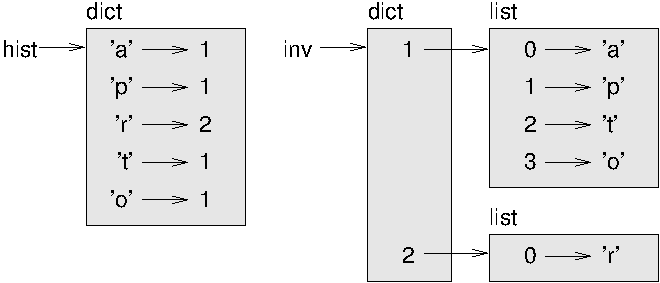
\includegraphics[scale=0.8]{figs/dict1.pdf}}
\caption{状态图.}
\label{fig.dict1}
\end{figure}

图~\ref{fig.dict1} 是表示 {\tt hist}和 {\tt inverse}的状态图. 
字典用箱体表示, 其上有{\tt dict}类型标识, 其内是键值对. 
通常如果值是整数, 浮点数或者字符串, 我会将其绘制在箱体内部, 
但如果是列表, 我会绘制在箱体外部, 只是为了简单易懂. 
\index{state diagram}
\index{diagram!state}

列表可以是字典的值, 就像图中所示, 但是不能作为键使用. 
下面是擅自使用遇到的错误:
\index{TypeError}
\index{exception!TypeError}


\begin{verbatim}
>>> t = [1, 2, 3]
>>> d = dict()
>>> d[t] = 'oops'
Traceback (most recent call last):
  File "<stdin>", line 1, in ?
TypeError: list objects are unhashable
\end{verbatim}
%
以前我讲过, 字典的实现基于哈希表, 意味着其键必须是{\bf 可散列的}.
\index{hash function}
\index{hashable}

{\bf hash}是一个函数, 其接收任意值(任何类型), 然后返回一个整数. 
字典会用这些被称为哈希值的整数, 对键值对进行存储和查找. 
\index{immutability}

如果键不可变, 则一切正常. 
如果键像列表一样可变, 那么便不太妙了. 
比如, 你想创建个键值对, 
Python 计算键的哈希值, 并将其存储于相应的位置. 
如果你修改了键, 然后再次计算哈希值, 那么位置不同了. 
这时候, 相当于一个键对应了两个不同的位置, 或者说, 你无法找到
某个键了. 总之, 字典不能正常使用了. 

这也就是键必须要可哈希的原因, 以及为何像列表一样的可变类型不能用作键的
原因. 突破此限制的最简单方法是使用元组, 这个在下一章节会学到. 

因为字典是可变的, 所以不能用作键, 
但是{\em 可以}用作值. 

\section{缓存}
\label{memoize}

如果你已经学习了第~\ref{one.more.example}节的{\tt fibonacci}函数, 
你会发现, 随着参数越大, 函数运行时间越长. 而且, 耗时增长的速度很快. 
\index{fibonacci function}
\index{function!fibonacci}

若想理解其原由, 参考图~\ref{fig.fibonacci}, 此{\bf 调用图}展示了当
{\tt n=4}时{\tt fibonacci} 函数的调用情况:
\begin{figure}
\centerline
{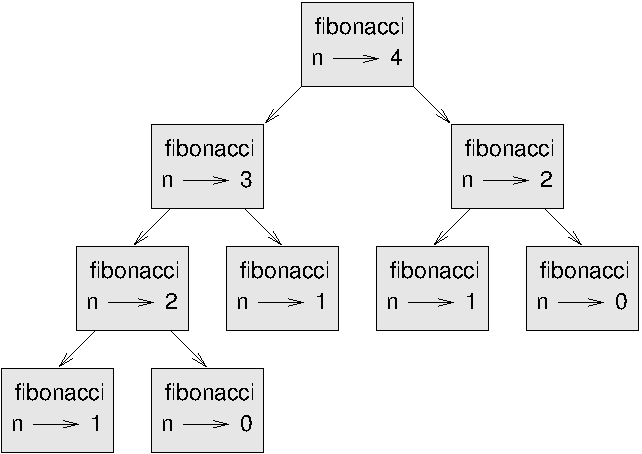
\includegraphics[scale=0.7]{figs/fibonacci.pdf}}
\caption{调用图.}
\label{fig.fibonacci}
\end{figure}
调用图是一堆函数框图, 用框与框间的连线, 表示调用关系. 
此图最顶层, 表示{\tt n=4}的{\tt fibonacci}函数会调用{\tt n=3}和{\tt n=2}时的函数. 
同样, {\tt n=3}时的{\tt fibonacci}函数会调用{\tt n=2}和{\tt n=1}时的函数, 
以此类推. 
\index{function frame}
\index{frame}
\index{call graph}

算算 {\tt fibonacci(0)} 和 {\tt fibonacci(1)} 会被调用多少次吧. 
此操作是如此低效, 而且随着参数变大, 效率更低. 
\index{memo}

另一种思路是跟踪并记录已经计算过的数据, 将其存储到字典中. 
将之前计算过的值存储起来, 方便后续使用, 这种操作叫做{\bf 缓存}.
下面是 {\tt fibonacci}的``缓存''版本:

\begin{verbatim}
known = {0:0, 1:1}

def fibonacci(n):
    if n in known:
        return known[n]

    res = fibonacci(n-1) + fibonacci(n-2)
    known[n] = res
    return res
\end{verbatim}
%
字典{\tt known} 用来跟踪记录过往结果. 
其初始包括两项: 0对应0, 1对应1.

每次{\tt fibonacci}被调用, 总会先检查{\tt known}. 
如果结果已经存在, 则立刻返回结果. 否则, 计算结果, 
并保存到字典, 然后返回结果. 

当你运行这个版本的{\tt fibonacci}, 和以前版本相比, 
你会发现, 快了很多. 


\section{全局变量}
\index{global variable}
\index{variable!global}
上例中, {\tt known} 是在函数外创建, 
所以它属于\verb"__main__"函数的框内, 这是一个特殊的框. 
\verb"__main__"函数中的变量, 有时也被认为是{\bf 全局的}, 
因为可以从任意函数访问它们. 
不像局部变量, 其运行的函数一旦结束, 便会消失, 
全局变量可以在一个函数执行到另一个函数时, 也保持存在. 
\index{flag}
\index{main}

全局变量, 一个常用的地方, 便是作为{\bf 标识}使用;
也就是作为布尔变量, 来表示(``标识'')条件是否成立. 
比如, 有些程序会使用 {\tt verbose}作为标识, 来控制输出信息的
详细程度:

\begin{verbatim}
verbose = True

def example1():
    if verbose:
        print('Running example1')
\end{verbatim}
%
如果尝试重新赋值全局变量, 可能会得到意外结果. 
下面的例子, 用全局变量来跟踪函数是否被调用过:
\index{reassignment}

\begin{verbatim}
been_called = False

def example2():
    been_called = True         # WRONG
\end{verbatim}
%
运行此程序, 你会注意到\verb"been_called"的值没有改变. 
问题在于 {\tt example2} 内部又创建了名为\verb"been_called"的局部变量. 
而局部变量会在函数结束后释放, 并不会对全局变量产生影响. 
\index{global statement}
\index{statement!global}
\index{declaration}

如果想在函数内部修改全局变量, 你需要在赋值前, {\bf 声明}这是全局变量:

\begin{verbatim}
been_called = False

def example2():
    global been_called 
    been_called = True
\end{verbatim}
%
这个{\bf global 声明}会告诉解释器,  ``在这个函数中, 当我说\verb"been_called", 
我指的是那个全局变量;而不是新建一个局部变量. ''
\index{update!global variable}
\index{global variable!update}

下面是段修改全局变量的代码:

\begin{verbatim}
count = 0

def example3():
    count = count + 1          # WRONG
\end{verbatim}
%
运行后, 你会看到:
\index{UnboundLocalError}
\index{exception!UnboundLocalError}

\begin{verbatim}
UnboundLocalError: local variable 'count' referenced before assignment
\end{verbatim}
%
Python假设{\tt count}是局部的, 据此假设, 需要在更新变量前先读取变量. 
解决方法依然是, 声明{\tt count}为全局变量. 
\index{counter}

\begin{verbatim}
def example3():
    global count
    count += 1
\end{verbatim}
%
如果全局变量指向了可变的值, 那你在修改前, 无需声明全局变量:
\index{mutability}

\begin{verbatim}
known = {0:0, 1:1}

def example4():
    known[2] = 1
\end{verbatim}
%
所以你可以在全局的列表或字典中, 添加, 移除以及替换元素, 
但是你若想对变量重新赋值, 需要提前声明全局变量:

\begin{verbatim}
def example5():
    global known
    known = dict()
\end{verbatim}
%
全局变量是很有用, 但如果你到处使用, 并且还频繁修改, 那么程序往往会
难以调试. 


\section{调试}
\index{debugging}
随着数据集越来越大, 仅仅使用打印输出以及手工校验结果的手段进行调试, 略显不便. 
下面是调试大型数据集的一些建议:

\begin{description}

\item[降低输入规模:] 如果可能, 降低数据集大小. 比如, 读取文本文件, 
只读取前10行, 或者使用你能找到的最简样例. 
可以重新编辑文件, 或者(更优的做法是)修改程序, 只读取前{\tt n}行. 

如果报错, 可以将{\tt n}减小为刚好会报错的最小值, 
然后修正异常, 并逐步增大{\tt n}值, 如此循环往复. 

\item[检验概览及类型:] 不要打印并检验全部数据集, 只需输出数据的概览:
比如, 字典中项的个数, 或者列表中数字总数量. 

值类型错误, 是产生运行时错误的常见原因. 
所以调试此类错误, 通常打印值的类型即可. 

\item[编写自检代码:]  有时候, 你可以编写代码, 自动检验异常. 
例如, 你要计算数字列表的平均值, 你可以检验一下, 结果是否
比列表中最大值还要大, 或者比最小值还要小. 这叫做``合理性检验'', 
是因为要检查结果是否``不合理''.  
\index{sanity check}
\index{consistency check}

另一种检验方法是比较两种不同解法的结果, 看是否一致. 
这叫做``一致性检验''. 

\item[格式化输出:] 格式化调试的输出, 可以更直观地展示错误. 
在第~\ref{factdebug}节, 我们曾展示过样例. 另一个好用的工具是 {\tt pprint} 模块, 
它提供了{\tt pprint}函数, 可以将内置类型输出为更适合人类阅读的格式({\tt pprint}
是``pretty pprint'' 的缩写).
\index{pretty print}
\index{pprint module}
\index{module!pprint}

\end{description}

再次强调, 构建脚手架花费时间越长, 调试耗费时间越少. 
\index{scaffolding}


\section{术语表}

\begin{description}

\item[映射(mapping):] 集合中每个元素都对应到另一个集合的单一元素的关系.
\index{mapping}

\item[字典(dictionary):] 从键到相应的值的映射. 
\index{dictionary}

\item[键值对(key-value pair):] 键到值的映射关系的表示. 
\index{key-value pair}

\item[项(item):] 字典中, 键值对的别名. 
\index{item!dictionary}

\item[键(key):] 字典中的一个对象, 也是键值对的第一部分. 
\index{key}

\item[值(value):] 字典中的一个对象, 作为键值对的第二部分. 
这里的表示和以前用到的``值''相比, 更加具体. 
\index{value}

\item[实现(implementation):] 一种执行计算的方式. 
\index{implementation}

\item[哈希表(hashtable):] 实现Python字典的算法. 
\index{hashtable}

\item[哈希函数(hash function):] 哈希表使用的函数, 用来计算键的位置. 
\index{hash function}

\item[散列的(hashable):] 一种可以使用哈希函数的类型. 
不可变类型, 像整型, 浮点型和字符串型, 都是可散列的;
像列表和字典这种可变类型, 则不是. 
\index{hashable}

\item[查找(lookup):] 一种字典操作, 根据键查找对应的值.
\index{lookup}

\item[反向查找(reverse lookup):] 一种字典操作, 通过值来查找对应的一个或多个键.
\index{reverse lookup}

\item[raise语句(raise statement):]  主动抛出异常的语句.
\index{raise statement}
\index{statement!raise}

\item[单元素集(singleton):] 只包含一个元素的列表(或者其他序列).
\index{singleton}

\item[调用图(call graph):] 一种用来展示程序执行流程的图, 包括每步创建的框, 
以及从调用者指向被调用者的箭头. 
\index{call graph}
\index{diagram!call graph}

\item[备忘(memo):] 存储计算过的值, 避免后续重复计算的操作. 
\index{memo}

\item[全局变量(global variable):] 定义在函数之外的变量. 
全局变量可以被任何函数获取使用. 
\index{global variable}

\item[global语句(global statement):] 声明变量是全局变量的语句.
\index{global statement}
\index{statement!global}

\item[标识(flag):] 标识条件是否为真的布尔变量. 
\index{flag}

\item[声明(declaration):] 像{\tt global}一样的语句, 用来告知解释器
变量的有关信息. 
\index{declaration}

\end{description}


\section{习题集}

\begin{exercise}
\label{wordlist2}
\index{set membership}
\index{membership!set}

编写函数, 读取{\tt words.txt}中的单词, 
将其作为键存储于字典中. 值是什么无关紧要. 
然后便可以用{\tt in}运算符快速检验某个字符串是否在字典中. 

如果你做过习题~\ref{wordlist1}, 可以比较一下这种实现, 和列表的{\tt in}运算, 
以及二分查找相比, 速度如何. 

\end{exercise}


\begin{exercise}
\label{setdefault}
阅读字典方法 {\tt setdefault}的文档, 
以此精简\verb"invert_dict"版本. 
参见: \url{http://thinkpython2.com/code/invert_dict.py}.
\index{setdefault method}
\index{method!setdefault}

\end{exercise}


\begin{exercise}
用缓存的方式重写习题~\ref{ackermann} 中的Ackermann函数, 
看看是否缓存方式可以使其处理较大参数. 
提示: 不能.
参考: \url{http://thinkpython2.com/code/ackermann_memo.py}.
\index{Ackermann function}
\index{function!ack}

\end{exercise}


\begin{exercise}
\index{duplicate}
如果做过习题~\ref{duplicate}, 你应该已经写过一个\verb"has_duplicates" 函数, 
令其接收一个列表作为参数, 如果其中存在任意重复对象, 则返回{\tt True}.

使用字典来编写一个更简单高效的\verb"has_duplicates"版本. 
参考: \url{http://thinkpython2.com/code/has_duplicates.py}.
\end{exercise}


\begin{exercise}
\label{exrotatepairs}
\index{letter rotation}
\index{rotation!letters}

两个单词, 如果翻转其中一个, 得到另一个, 则称其为``翻转词组''
(参见习题~\ref{exrotate}中的\verb"rotate_word" ).

编写程序读取一个单词表, 并找到所有的翻转词组. 
参考: \url{http://thinkpython2.com/code/rotate_pairs.py}.

\end{exercise}


\begin{exercise}
\index{Car Talk}
\index{Puzzler}

这是另一个来自{\em Car Talk}的迷题
(\url{http://www.cartalk.com/content/puzzlers}):

\begin{quote}
这个谜题来自于一个名为Dan O'Leary的朋友. 
他最近发现一个单音节, 五个字母的常用单词, 其具有下述特征. 
当你移除首字母, 剩下字母构成了一个和原单词发音完全一样的同音词. 
如果再替换首字母, 也就是把首字母放回去, 移除第二个字母, 然后得到的又是
同音词. 那么问题来了, 这是什么词?

现在, 我给你展示一个错误的例子. 
咱们看一下这个五个字母的单词, `wrack'.  W-R-A-C-K, 就是
`wrack with pain.' 中的那个`wrack'. 
如果移除首字母, 剩下四个字母的单词, 'R-A-C-K.' 
比如, `Holy cow, did you see the rack on that buck!
It must have been a nine-pointer!' 发音完全一样. 
如果你放回`w', 移除`r', 得到一个单词, `wack', 
这是一个真正的单词, 只是发音和前两个不同. 

但是, 至少有一个这样的单词, Dan和我们都认识, 
分别删除前两个字母, 构成两个新的四个字母单词, 发音完全相同. 
问题是, 这个词是什么?
\end{quote}
\index{homophone}
\index{reducible word}
\index{word, reducible}

你可以用习题~\ref{wordlist2} 中的字典来检验一个字符串是否在单词表中. 

若想检查两个单词是否是同音词, 可以用CMU发音词典. 
这个词典可以从\url{http://www.speech.cs.cmu.edu/cgi-bin/cmudict}
或\url{http://thinkpython2.com/code/c06d}下载. 
或者下载\url{http://thinkpython2.com/code/pronounce.py}代码, 
这个文件提供了一个 \verb"read_dictionary"函数, 
可以读取发音词典并返回一个Python字典, 此字典将每个单词映射到了
表示发音的字符串. 

编写程序列出所有满足谜语条件的单词. 
答案: \url{http://thinkpython2.com/code/homophone.py}.

\end{exercise}



\chapter{元组}
\label{tuplechap}

本章介绍另一种内置类型, 元组, 以及列表、字典和元组如何一起使用. 
同时展示可变长度参数列表的一个特性, 以及聚合和扩展运算符. 

话外音: 对于 ``tuple''如何发音, 尚无共识. 有人读``tuh-ple'', 
和 ``supple''发音类系. 
但在编程领域, 多数人读``too-ple'', 和``quadruple''发音一样. 


\section{元组不可变}
\index{tuple}
\index{type!tuple}
\index{sequence}

元组也是值的序列. 其中值可以是任意类型, 也是用整数作为索引, 
所以在某些方面, 元组和列表很像. 
但两者最大的区别在于元组不可变. 
\index{mutability}
\index{immutability}

从语法来看, 元组就是一个逗号分隔的序列:

\begin{verbatim}
>>> t = 'a', 'b', 'c', 'd', 'e'
\end{verbatim}
%
虽然不是很必要, 但一般都用括号把元组括起来:
\index{parentheses!tuples in}

\begin{verbatim}
>>> t = ('a', 'b', 'c', 'd', 'e')
\end{verbatim}
%
若要创建一个单元素的元组, 需要在末尾加上逗号:
\index{singleton}
\index{tuple!singleton}

\begin{verbatim}
>>> t1 = 'a',
>>> type(t1)
<class 'tuple'>
\end{verbatim}
%
括号中只有一个值, 便不是元组:

\begin{verbatim}
>>> t2 = ('a')
>>> type(t2)
<class 'str'>
\end{verbatim}
%
另一种创建元组的方法, 可以使用内置函数{\tt tuple}. 
如果不传参数, 便会创建一个空元组:
\index{tuple function}
\index{function!tuple}

\begin{verbatim}
>>> t = tuple()
>>> t
()
\end{verbatim}
%
如果参数是一个序列(字符串, 列表或者元组), 
结果便会得到一个由元素序列构成的元组:

\begin{verbatim}
>>> t = tuple('lupins')
>>> t
('l', 'u', 'p', 'i', 'n', 's')
\end{verbatim}
%
因为{\tt tuple} 是一个内置函数名, 
所以要尽量避免用作变量名. 

多数列表运算符同样适用于元组. 
所以用方括号也可以索引元组元素:
\index{bracket operator}
\index{operator!bracket}

\begin{verbatim}
>>> t = ('a', 'b', 'c', 'd', 'e')
>>> t[0]
'a'
\end{verbatim}
%
切片运算符也可以选择元组中一段区间的元素. 
\index{slice operator}
\index{operator!slice}
\index{tuple!slice}
\index{slice!tuple}

\begin{verbatim}
>>> t[1:3]
('b', 'c')
\end{verbatim}
%
你如果想修改元组中的某个元素, 会报错:
\index{exception!TypeError}
\index{TypeError}
\index{item assignment}
\index{assignment!item}

\begin{verbatim}
>>> t[0] = 'A'
TypeError: object doesn't support item assignment
\end{verbatim}
%
因为元组不可变, 所以你不能修改其中元素. 
但是你可以用另一个元组替换当前元组:

\begin{verbatim}
>>> t = ('A',) + t[1:]
>>> t
('A', 'b', 'c', 'd', 'e')
\end{verbatim}
%
这个语句创建新元组, 然后用 {\tt t} 指向它. 

关系运算符也同样适用于元组以及其他序列;
Python会从各自序列的首元素开始比较, 如果相等, 则比较下一个元素, 
以此类推, 直到找出不同元素. 
而后续元素便不再比较(即使后面元素更大). 
\index{comparison!tuple}
\index{tuple!comparison}

\begin{verbatim}
>>> (0, 1, 2) < (0, 3, 4)
True
>>> (0, 1, 2000000) < (0, 3, 4)
True
\end{verbatim}



\section{元组赋值}
\label{tuple.assignment}
\index{tuple!assignment}
\index{assignment!tuple}
\index{swap pattern}
\index{pattern!swap}
交换变量的值经常会用到. 
比较传统的方法, 是使用中间变量. 
比如下面例子, 互换 {\tt a} 和 {\tt b}的值:

\begin{verbatim}
>>> temp = a
>>> a = b
>>> b = temp
\end{verbatim}
%
这种方法比较麻烦; 用{\bf 元组赋值}会优雅很多:

\begin{verbatim}
>>> a, b = b, a
\end{verbatim}
%
左侧是个变量元组;右侧是个表达式元组. 
每个值都会赋值给其对应的变量. 
右侧的表达式在赋值操作前都会先计算. 

同时左侧变量的数量必须要和右侧值的数量一样:
\index{exception!ValueError}
\index{ValueError}

\begin{verbatim}
>>> a, b = 1, 2, 3
ValueError: too many values to unpack
\end{verbatim}
%
也有更普遍的用法, 右侧可以用各种类型的序列(字符串, 列表或者元组). 
例如, 将一个邮箱地址切分为用户名和域名, 可以这么写:
\index{split method}
\index{method!split}
\index{email address}

\begin{verbatim}
>>> addr = 'monty@python.org'
>>> uname, domain = addr.split('@')
\end{verbatim}
%
{\tt split}的结果是一个两元素的列表;
第一个元素赋值给了{\tt uname}, 第二个赋值给了{\tt domain}. 

\begin{verbatim}
>>> uname
'monty'
>>> domain
'python.org'
\end{verbatim}
%

\section{元组作为返回值}
\index{tuple}
\index{value!tuple}
\index{return value!tuple}
\index{function!tuple as return value}
严格来讲, 函数只能返回一个值, 但是如果这个值是一个元组, 
效果便等同于返回了多个值. 
比如, 你要将两个整数相除, 计算商和余数, 先计算{\tt x//y} , 再
计算{\tt x\%y}, 略显低效. 更好的方法是同时计算两个值. 
\index{divmod}

内置函数 {\tt divmod} 会接收两个参数, 返回一个包含两个值的元组, 
商和余数. 同时, 你也可以将结果存储为元组:

\begin{verbatim}
>>> t = divmod(7, 3)
>>> t
(2, 1)
\end{verbatim}
%
或者用元组赋值分别存储结果:
\index{tuple assignment}
\index{assignment!tuple}

\begin{verbatim}
>>> quot, rem = divmod(7, 3)
>>> quot
2
>>> rem
1
\end{verbatim}
%
下面是一个返回元组的函数:

\begin{verbatim}
def min_max(t):
    return min(t), max(t)
\end{verbatim}
%
{\tt max} 和 {\tt min} 都是内置函数,  用来从序列中寻找最大值和最小值. 
\verb"min_max"函数计算两者, 然后将其作为元组返回. 
\index{max function}
\index{function!max}
\index{min function}
\index{function!min}


\section{变长参数即元组}
\label{gather}
\index{variable-length argument tuple}
\index{argument!variable-length tuple}
\index{gather}
\index{parameter!gather}
\index{argument!gather}
函数可以接收任意数量参数. 以{\tt *} 开头的参数会{\bf 聚合}所有参数作为一个元组. 
比如, {\tt printall}会接收任意数量的参数, 并打印输出:

\begin{verbatim}
def printall(*args):
    print(args)
\end{verbatim}
%
这个聚合参数可以随意命名, 但是 {\tt args}更为人所熟知. 
下面的函数展示其效果:

\begin{verbatim}
>>> printall(1, 2.0, '3')
(1, 2.0, '3')
\end{verbatim}
%
聚合的对立面是{\bf 扩展}. 
如果你有一个值的序列, 想将其作为多个参数, 传入函数, 那便可以使用{\tt *}运算符. 
比如, {\tt divmod}仅接收两个参数; 如果传入一个元组, 则运行异常:
\index{scatter}
\index{argument scatter}
\index{TypeError}
\index{exception!TypeError}

\begin{verbatim}
>>> t = (7, 3)
>>> divmod(t)
TypeError: divmod expected 2 arguments, got 1
\end{verbatim}
%
但如果你扩展了元组, 那便运行正常:

\begin{verbatim}
>>> divmod(*t)
(2, 1)
\end{verbatim}
%
很多内置函数都会用到变长参数元组. 
比如, {\tt max}和{\tt min}都可以接收任意数量的参数:
\index{max function}
\index{function!max}
\index{min function}
\index{function!min}

\begin{verbatim}
>>> max(1, 2, 3)
3
\end{verbatim}
%
但{\tt sum}函数不行.
\index{sum function}
\index{function!sum}

\begin{verbatim}
>>> sum(1, 2, 3)
TypeError: sum expected at most 2 arguments, got 3
\end{verbatim}
%
做个练习, 写个函数 \verb"sum_all", 使其可以接收任意数量参数, 并返回总和. 


\section{列表和元组}
\index{zip function}
\index{function!zip}
{\tt zip}是个内置函数,  其接收两个或者更多序列作为参数, 并交错获取其中元素. 
这个函数的名字表示其像拉链, 仿若两排交错的牙齿. 

下面的例子是压缩一个字符串和一个列表:

\begin{verbatim}
>>> s = 'abc'
>>> t = [0, 1, 2]
>>> zip(s, t)
<zip object at 0x7f7d0a9e7c48>
\end{verbatim}
%
结果是个 {\bf zip 对象}, 用来迭代数值对. 
所以{\tt zip}常常用在{\tt for}循环内:

\begin{verbatim}
>>> for pair in zip(s, t):
...     print(pair)
...
('a', 0)
('b', 1)
('c', 2)
\end{verbatim}
%

zip对象是一种{\bf 迭代器}, 也就是一种用来迭代序列的对象. 
迭代器和列表在某些方面比较相似, 但与列表不同的是, 你不能从
迭代器中通过索引获取元素. 
\index{iterator}

如果你想使用列表的运算符和方法, 可以用zip对象构建列表:

\begin{verbatim}
>>> list(zip(s, t))
[('a', 0), ('b', 1), ('c', 2)]
\end{verbatim}
%
列表中都是元组; 在这个例子中, 每个元组都包括
字符串中的一个字母, 以及列表中的相应元素. 
\index{list!of tuples}

若序列长度不同, 则结果长度取决于较短的那个序列. 

\begin{verbatim}
>>> list(zip('Anne', 'Elk'))
[('A', 'E'), ('n', 'l'), ('n', 'k')]
\end{verbatim}
%
可以在{\tt for}循环中使用元组赋值, 遍历元组列表:
\index{traversal}
\index{tuple assignment}
\index{assignment!tuple}

\begin{verbatim}
t = [('a', 0), ('b', 1), ('c', 2)]
for letter, number in t:
    print(number, letter)
\end{verbatim}
%
每次循环, Python都会获取列表中的下一个元组, 并将其元素分别
赋给 {\tt letter} 和 {\tt number}. 
循环的输出如下:
\index{loop}

\begin{verbatim}
0 a
1 b
2 c
\end{verbatim}
%
如果结合 {\tt zip}, {\tt for} 和元组赋值, 那你便得到了一个同时
遍历两个(或多个)序列的利器. 比如, \verb"has_match" 接收两个序列, 
{\tt t1} 和 {\tt t2}, 如果存在索引{\tt i}, 令{\tt t1[i] == t2[i]}成立, 
则返回 {\tt True}:
\index{for loop}

\begin{verbatim}
def has_match(t1, t2):
    for x, y in zip(t1, t2):
        if x == y:
            return True
    return False
\end{verbatim}
%
如果你需要遍历序列元素以及其索引, 可以使用
内置函数{\tt enumerate}:
\index{traversal}
\index{enumerate function}
\index{function!enumerate}

\begin{verbatim}
for index, element in enumerate('abc'):
    print(index, element)
\end{verbatim}
%
 {\tt enumerate} 返回的结果是一个枚举对象, 
会迭代一个值对序列;
每个值对包括索引(从0开始)和给定序列中的元素. 
此例输出同样如下:

\begin{verbatim}
0 a
1 b
2 c
\end{verbatim}
%
\index{iterator}
\index{object!enumerate}
\index{enumerate object}


\section{字典和元组}
\label{dictuple}
\index{dictionary}
\index{items method}
\index{method!items}
\index{key-value pair}

字典有个方法叫做{\tt items}, 其返回一个元组序列, 每个元组都是一个键值对.

\begin{verbatim}
>>> d = {'a':0, 'b':1, 'c':2}
>>> t = d.items()
>>> t
dict_items([('c', 2), ('a', 0), ('b', 1)])
\end{verbatim}
%
结果是个 \verb"dict_items" 对象, 是一个迭代键值对的迭代器. 
可以在 {\tt for} 中使用, 如下所示:
\index{iterator}

\begin{verbatim}
>>> for key, value in d.items():
...     print(key, value)
...
c 2
a 0
b 1
\end{verbatim}
%
如你所想, 字典中的项没有特定顺序. 

相反, 你也可以用一个元组列表, 初始化一个新字典: 
\index{dictionary!initialize}

\begin{verbatim}
>>> t = [('a', 0), ('c', 2), ('b', 1)]
>>> d = dict(t)
>>> d
{'a': 0, 'c': 2, 'b': 1}
\end{verbatim}

将{\tt dict}和{\tt zip}结合使用, 便产生了一种新建字典的简洁方法:
\index{zip function!use with dict}

\begin{verbatim}
>>> d = dict(zip('abc', range(3)))
>>> d
{'a': 0, 'c': 2, 'b': 1}
\end{verbatim}
%
字典的{\tt update}方法也可以接收一个元组列表, 然后将其
作为键值对添加到已有字典中.
\index{update method}
\index{method!update}
\index{traverse!dictionary}
\index{dictionary!traversal}

使用元组作为字典的键, 很常见(主要是列表不能). 
比如, 电话簿会将姓氏-名字映射到电话号码. 
假设我们定义了{\tt last}, {\tt first} 和 {\tt number}, 
便可以编写如下:
\index{tuple!as key in dictionary}
\index{hashable}

\begin{verbatim}
directory[last, first] = number
\end{verbatim}
%
方括号中的表达式是个元组. 
可以用元组赋值语句来遍历字典.
\index{tuple!in brackets}

\begin{verbatim}
for last, first in directory:
    print(first, last, directory[last,first])
\end{verbatim}
%
此循环会遍历 {\tt directory}中的键, 也就是元组. 
同时会将元组中的元素赋值给{\tt last} 和 {\tt first}, 
然后输出姓名以及对应的电话号码. 

在状态图中展示元组有两种方法. 
较详细的版本会展示起索引和元素, 就像列表一样. 
例如, 图~\ref{fig.tuple1} 展示了元组 \verb"('Cleese', 'John')" .
\index{state diagram}
\index{diagram!state}

\begin{figure}
\centerline
{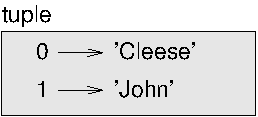
\includegraphics[scale=0.8]{figs/tuple1.pdf}}
\caption{状态图.}
\label{fig.tuple1}
\end{figure}

但在大规模得图中, 你需要忽略细节. 
图~\ref{fig.dict2}展示了电话簿的状态.

\begin{figure}
\centerline
{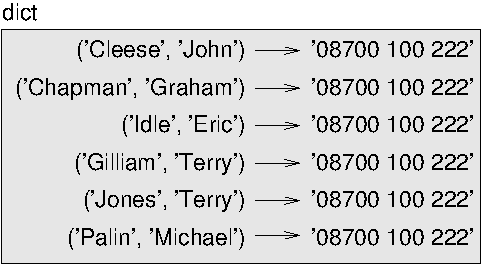
\includegraphics[scale=0.8]{figs/dict2.pdf}}
\caption{状态图.}
\label{fig.dict2}
\end{figure}

图中的元组都使用Python语法形象表示. 
电话号码是BBC的投诉热线, 所以请不要拨打. 


\section{序列中的序列}
\index{sequence}

我一直讲的是元组列表, 但是本章几乎所有示例同样适用于
列表构成的列表, 元组构成的元组, 以及列表构成的元组. 
为了避免枚举各种组合, 直接叫做序列构成的序列, 便简单多了. 

很多情形下, 不同类型的序列(字符串, 列表以及元组)可以替换使用, 
那你如何从中择优呢?
\index{string}
\index{list}
\index{tuple}
\index{mutability}
\index{immutability}

从最显而易见的情形考虑, 字符串比其他序列, 应用场景最有限, 
因为其元素需要是字符. 
同时, 他们不能被修改. 
如果你想要修改字符串中的字符(而不是新建一个新字符串), 
你最好还是用字符列表吧. 

列表比元组更加常用, 主要因为列表可变. 
但以下情况, 用元组会更好:

\begin{enumerate}

\item 在某些情形, 比如{\tt return}语句, 语法上创建元组比创建列表更简便. 

\item 如果你想使用序列作为字典的键, 
你需要使用元组或者字符串这种不可变类型. 

\item 如果需要将一个序列作为参数传递给函数, 
使用元组可以有效降低使用别名带来的潜在问题. 

\end{enumerate}

因为元组不可变, 所以它们不提供 {\tt sort} 和 {\tt reverse}这种修改现有列表的方法, 
但是Python提供内置函数 {\tt sorted}, 其接收任意序列, 然后返回一个排序后的新列表, 
也提供了{\tt reversed}函数, 其接收一个序列, 返回一个迭代器, 此迭代器可以
倒序遍历列表. 
\index{sorted function}
\index{function!sorted} \index{reversed function}
\index{function!reversed}
\index{iterator}


\section{调试}
\index{debugging}
\index{data structure}
\index{shape error}
\index{error!shape}

列表, 字典以及元组都是 {\bf 数据结构}的例子;
本章我们开始了解复合数据结构, 像元组列表, 或者用元组作键, 
列表作值的字典. 
复合数据结构很有用, 但很容易产生我说的{\bf 格式异常};
就是当数据结构中出现了不恰当的类型, 大小或结构, 导致的错误. 
比如, 你想要一个含有一个整数的列表, 而我给了一个单纯的整数
(不被列表包含), 那便会出错. 
\index{structshape module}
\index{module!structshape}

为了调试这种异常, 我写了一个叫作 {\tt structshape} 的模块, 
其提供了一个{\tt structshape}函数, 可以接收任意数据结构作为参数, 
返回一个其格式的概述. 
你可以从 \url{http://thinkpython2.com/code/structshape.py} 下载. 

下面是一个简单列表的示范:

\begin{verbatim}
>>> from structshape import structshape
>>> t = [1, 2, 3]
>>> structshape(t)
'list of 3 int'
\end{verbatim}
%

严谨点的写法是``list of 3 int{\em s}'', 
但是忽略复数, 便于操作. 下面是一个列表构成的列表:

\begin{verbatim}
>>> t2 = [[1,2], [3,4], [5,6]]
>>> structshape(t2)
'list of 3 list of 2 int'
\end{verbatim}
%
如果列表中的元素类型不止一种, 
{\tt structshape} 按顺序汇总类型:

\begin{verbatim}
>>> t3 = [1, 2, 3, 4.0, '5', '6', [7], [8], 9]
>>> structshape(t3)
'list of (3 int, float, 2 str, 2 list of int, int)'
\end{verbatim}
%
这是一个元组列表:

\begin{verbatim}
>>> s = 'abc'
>>> lt = list(zip(t, s))
>>> structshape(lt)
'list of 3 tuple of (int, str)'
\end{verbatim}
%
下面是一个包含3个项的字典, 每个项都是映射整数到字符串.

\begin{verbatim}
>>> d = dict(lt) 
>>> structshape(d)
'dict of 3 int->str'
\end{verbatim}
%
如果你对你的数据结构感到棘手, 可以试试{\tt structshape}.


\section{术语表}

\begin{description}

\item[元组(tuple):] 一个不可变的元素序列. 
\index{tuple}

\item[元组赋值(tuple assignment):] 一种序列居右, 变量元组在左的赋值语句. 
等号右侧会先运算, 然后这些结果会赋值给相应的左侧变量. 
\index{tuple assignment}
\index{assignment!tuple}

\item[聚合(gather):] 将多个参数聚合为一个元组的操作.
\index{gather}

\item[扩展(scatter):] 使序列表现为多个参数的操作. 
\index{scatter}

\item[zip对象(zip object):] 调用内置函数{\tt zip}返回的结果;
是可遍历多个元组序列的对象. 
\index{zip object}
\index{object!zip}

\item[迭代器(iterator):] 可遍历序列的对象, 但不适用列表运算符和方法. 
\index{iterator}

\item[数据结构(data structure):] 相关值的集合, 通常由列表, 字典, 元组等组成. 
\index{data structure}

\item[格式异常(shape error):] 值的格式不合适导致的错误, 通常是类型或者大小. 
\index{shape}

\end{description}


\section{习题集}

\begin{exercise}

编写函数 \verb"most_frequent", 接收一个字符串, 然后按照字母频数倒序输出. 
从不同语言找一些文本素材, 看看不同语言之间字母频数有何差异. 
并将结果与\url{http://en.wikipedia.org/wiki/Letter_frequencies}中的表格进行比较. 
参考:
\url{http://thinkpython2.com/code/most_frequent.py}.  
\index{letter frequency} 
\index{frequency!letter}

\end{exercise}


\begin{exercise}
\label{anagrams}
\index{anagram set}
\index{set!anagram}

再来些变位词!

\begin{enumerate}

\item 编写程序, 从文件中读取单词列表(参见第~\ref{wordlist}节), 
并且输出所有的变位词集合. 

下面是个输出样例:

\begin{verbatim}
['deltas', 'desalt', 'lasted', 'salted', 'slated', 'staled']
['retainers', 'ternaries']
['generating', 'greatening']
['resmelts', 'smelters', 'termless']
\end{verbatim}
%
提示: 你或许会想要构建个字典, 将字母集合映射到单词列表, 
而列表中的单词都可以用这些字母构成. 问题来了, 你如何表示这些字母集合, 
从而使其能够作为键来使用?

\item 修改上面的程序, 使其先输出最长的变位词, 然后输出次长, 依次类推. 
\index{Scrabble}
\index{bingo}

\item 拼字游戏中, 你已有7张牌了, 如果又翻出了第8张, 构成了一个8字母的单词, 那么
你就获得了一个``bingo''. 找找哪些8字母的组合, 是最可能获得``bingo''的组合?

% (7, ['angriest', 'astringe', 'ganister', 'gantries', 'granites',
% 'ingrates', 'rangiest'])

参考: \url{http://thinkpython2.com/code/anagram_sets.py}.

\end{enumerate}
\end{exercise}

\begin{exercise}
\index{metathesis}
如果将一个单词交换其中两个字母的位置, 构成另一个单词, 则这两个单词
构成了一个 ``易位词对''; 比如, ``converse'' 和 ``conserve''.  
编写程序, 从字典中寻找所有的``易位词对''.
提示: 不用尝试所有的单词组合, 也不用尝试所有可能易位操作. 
参考:
\url{http://thinkpython2.com/code/metathesis.py}.  
鸣谢: 这道题源自\url{http://puzzlers.org}上的一个例子. 
\end{exercise}


\begin{exercise}
\index{Car Talk}
\index{Puzzler}

这又是一个汽车广播字迷
(\url{http://www.cartalk.com/content/puzzlers}):

\begin{quote}
每次从单词中移除一个字母, 依然是正确的英文单词, 这样的单词中, 
最长的是哪个?

可以从末尾或者中间移除字母, 但不能调整任何字母的顺序. 
每次移除一个字母, 都得到一个新的英文单词. 一直这样操作, 
最终会得到一个字母, 同时这个字母也是一个英文单词---可以在字典中找到. 
那么最长的单词是什么, 以及它有多少个字母?

我举个小例子: Sprite. 认识吗? 从sprite开始, 从中间去掉一个字母, 移除r, 剩下的字母构成了单词 spite, 
然后移除末尾的字母, 得到单词 spit, 然后移除 s, 得到 pit, 然后依次得到 it, 和 I. 
\end{quote}
\index{reducible word}
\index{word, reducible}

编写程序, 寻找所有这样可以缩减的单词, 然后确定最长的单词. 

这道题相比其他题有些难, 所以这里给些提示:

\begin{enumerate}

\item 你可能需要写个函数, 接收一个单词, 然后计算得到所有的单词列表. 
这些单词都是通过移除一个字母得到. 这些就是这个单词的``子类''.
\index{recursive definition}
\index{definition!recursive}

\item 用递归思路来考虑, 如果一个单词的子类是可以缩减的, 
那么这个单词就是可以缩减的. 可以将空字符串可缩减, 作为基准条件. 

\item 我提供的单词列表 {\tt words.txt}, 不包含单字母单词. 所以你可能需要添加``I'', ``a''和空字符串. 

\item 若想提升程序性能, 最好缓存住已知的可缩减单词. 

\end{enumerate}

参考: \url{http://thinkpython2.com/code/reducible.py}.

\end{exercise}


%\begin{exercise}
%\url{http://en.wikipedia.org/wiki/Word_Ladder}
%\end{exercise}


\chapter{案例学习: 数据结构选择}

截止当前, 你已学习了Python最核心的数据结构, 
同时也已熟悉了与之相关的一些算法. 
若想后续深入了解算法知识, 可以学习章节~\ref{algorithms}. 
但现在不用太急切; 后续时间方便了, 可以耐心学习. 

本章通过多道习题, 一个案例来让你思考如何选择和应用数据结构. 


\section{词频统计}
\label{analysis}

同往常一样, 看答案前先尽量尝试自己做一下. 

\begin{exercise}

写个程序, 读取文件, 把每行拆分成单词, 去掉空格和标点, 并将其转为小写. 
\index{string module}
\index{module!string}

提示: {\tt string}模块提供了名为{\tt whitespace}和名为 
{\tt  punctuation}的字符串, {\tt whitespace}包含了空格, 制表符, 换行等等; 而{\tt punctuation} 则包含各种标点符号. 
让我们看看是否可以用Python来说明:

\begin{verbatim}
>>> import string
>>> string.punctuation
'!"#$%&\'()*+,-./:;<=>?@[\\]^_`{|}~'
\end{verbatim}
%
同时, 你可能会用到字符串方法{\tt strip},
{\tt replace} 和 {\tt translate}.
\index{strip method}
\index{method!strip}
\index{replace method}
\index{method!replace}
\index{translate method}
\index{method!translate}

\end{exercise}


\begin{exercise}
\index{Project Gutenberg}

前往Gutenberg项目 (\url{http://gutenberg.org}), 然后下载一个你最喜欢的书籍, 
要下载无版权书籍的纯文本格式. 
\index{plain text}
\index{text!plain}

修改上个习题的代码, 使其可以读取所下载书籍的内容, 同时跳过书籍开头部分的标题信息, 像以前一样处理其余单词. 

调整代码, 统计书中单词总数, 以及每个单词出现次数. 
\index{word frequency}
\index{frequency!word}

输出书中不重复的单词数量. 
比较不同作者在不同时代撰写的不同书籍, 看看哪个作者的用词最丰富?
\end{exercise}


\begin{exercise}

修改上面习题中的程序, 输出书中出现次数最多的20个单词. 

\end{exercise}


\begin{exercise}

修改上述代码, 使其读取单词列表(参见第~\ref{wordlist}节), 
并输出所有出现在书中, 但不在单词表中的词汇. 
看看有多少是拼写异常? 又有多少是{\em 应该}包含在单词表中的常用词汇,
又有哪些是晦涩难懂的单词?

\end{exercise}


\section{随机数}
\index{random number}
\index{number, random}
\index{deterministic}
\index{pseudorandom}

多数程序, 给定同样的输入, 每次都是同样的输出, 这就叫做{\bf 确定性}.
确定性是件好事, 因为我们总是希望同样的计算产生同样的结果. 
但对于某些应用来说, 我们需要计算机能变得不可预测. 
游戏就是一个很好的例子, 也有很多其他的应用场景. 

想让一个程序完全随机, 是很难的, 但是可以让其看起来随机. 
一种方法是使用算法生成{\bf 伪随机}数.
伪随机数不是真正随机的, 因为它们是用一个确定的运算生成的, 
但只是从数字来看, 很难与真随机进行区分. 
\index{random module}
\index{module!random}

{\tt random}模块提供了生成伪随机数(后续均用``随机数''作为简称)的函数.
\index{random function}
\index{function!random}

函数{\tt random}会返回0.0到1.0之间(包括0.0但不包括1.0)的一个随机浮点数. 
每次调用{\tt random}, 都会得到既定长序列上的下一个值. 
下面的循环便是一个例子:

\begin{verbatim}
import random

for i in range(10):
    x = random.random()
    print(x)
\end{verbatim}
%
函数{\tt randint}接收参数 {\tt low} 和{\tt high}, 
返回 {\tt low} 和 {\tt high} 之间的一个整数(包括两者). 
\index{randint function}
\index{function!randint}

\begin{verbatim}
>>> random.randint(5, 10)
5
>>> random.randint(5, 10)
9
\end{verbatim}
%
若想从一个序列随机选择一个元素, 可以用{\tt choice}函数:
\index{choice function}
\index{function!choice}

\begin{verbatim}
>>> t = [1, 2, 3]
>>> random.choice(t)
2
>>> random.choice(t)
3
\end{verbatim}
%
{\tt random}模块也提供了些可基于某种连续分布, 
比如高斯分布, 指数分布, 伽马分布等, 生成随机数的函数. 

\begin{exercise}
\index{histogram!random choice}

编写\verb"choose_from_hist"函数, 使其
以第~\ref{histogram}节中定义的统计频数为输入, 然后从中
根据与频数成正比的概率来返回一个随机数. 
比如, 对于下面的频数统计来说:

\begin{verbatim}
>>> t = ['a', 'a', 'b']
>>> hist = histogram(t)
>>> hist
{'a': 2, 'b': 1}
\end{verbatim}
%
你的函数应该返回\verb"'a'" 的概率是$2/3$,  返回\verb"'b'"的概率是$1/3$.
\end{exercise}


\section{词频}

继续下面章节前, 先尽量完成上面的练习. 
你可以从 \url{http://thinkpython2.com/code/analyze_book1.py}下载
我的解决方案. 此外, 你也会需要\url{http://thinkpython2.com/code/emma.txt}这个文件.

下面是一个读取文件, 并基于其中单词构建词频统计的程序:
\index{histogram!word frequencies}

\begin{verbatim}
import string

def process_file(filename):
    hist = dict()
    fp = open(filename)
    for line in fp:
        process_line(line, hist)
    return hist

def process_line(line, hist):
    line = line.replace('-', ' ')
    
    for word in line.split():
        word = word.strip(string.punctuation + string.whitespace)
        word = word.lower()
        hist[word] = hist.get(word, 0) + 1

hist = process_file('emma.txt')
\end{verbatim}
%
这个程序会读取 {\tt emma.txt}, 其中包括了Jane Austen的{\em Emma}小说. 
\index{Austen, Jane}

\verb"process_file" 遍历文件中的每一行, 同时将每行内容逐次传给\verb"process_line". 
词频{\tt hist} 在此处作为累加器使用. 
\index{accumulator!histogram}
\index{traversal}

\verb"process_line"用字符串方法{\tt replace}将连字符替换为空格, 然后用
 {\tt split}方法, 将整行拆分为字符串列表. 
然后遍历列表, 并使用{\tt strip}方法, 移除标点符号, 使用{\tt lower}方法, 
转换为全小写. (此处简单说是``转换'', 但要记住字符串是不可变的, 所以像
{\tt strip}以及{\tt lower} 方法, 都是返回新的字符串.)

最终, \verb"process_line" 会通过新建项或者累加已有项, 更新词频统计.
\index{update!histogram}

若想统计文件中全部单词数量, 可以将词频统计中的所有频数相加求和即可:

\begin{verbatim}
def total_words(hist):
    return sum(hist.values())
\end{verbatim}
%
不同单词的数量也就是字典中项的数量:

\begin{verbatim}
def different_words(hist):
    return len(hist)
\end{verbatim}
%
下面的代码会输出结果:

\begin{verbatim}
print('Total number of words:', total_words(hist))
print('Number of different words:', different_words(hist))
\end{verbatim}
%
结果如下:

\begin{verbatim}
Total number of words: 161080
Number of different words: 7214
\end{verbatim}
%

\section{最常用单词}

若想找到最常用的单词, 我们可以创建一个元组列表, 
每个元组都包含一个单词和其频数, 然后据此将列表排序.

下面函数接收一个词频统计, 然后返回一个词-频元组列表:

\begin{verbatim}
def most_common(hist):
    t = []
    for key, value in hist.items():
        t.append((value, key))

    t.sort(reverse=True)
    return t
\end{verbatim}

每个元组中, 频数在前, 所以列表便是按频数排序. 
下面循环会输出前十个最常用单词:

\begin{verbatim}
t = most_common(hist)
print('The most common words are:')
for freq, word in t[:10]:
    print(word, freq, sep='\t')
\end{verbatim}
%
此处使用用关键词参数{\tt sep}, 来令{\tt print} 用换表符而不是空格作为``分隔符'', 
这样第二列就会对齐.  下面是对{\em Emma}小说的统计结果:

\begin{verbatim}
The most common words are:
to      5242
the     5205
and     4897
of      4295
i       3191
a       3130
it      2529
her     2483
was     2400
she     2364
\end{verbatim}
%
上述代码可以用 {\tt sort}函数的{\tt key}参数来简化. 
如果你感兴趣, 可以参阅 \url{https://wiki.python.org/moin/HowTo/Sorting}.


\section{可选参数}
\index{optional parameter}
\index{parameter!optional}
我们已经见到了诸多具有可选参数的内置函数和方法. 
而且我们也可以编写具有可选参数的自定义函数. 
比如, 下面是输出词频统计中最常用单词的函数:
\index{programmer-defined function}
\index{function!programmer defined}

\begin{verbatim}
def print_most_common(hist, num=10):
    t = most_common(hist)
    print('The most common words are:')
    for freq, word in t[:num]:
        print(word, freq, sep='\t')
\end{verbatim}

第一个参数是不可或缺的; 第二个是可选的. 
{\tt num}的{\bf 默认值}是10.
\index{default value}
\index{value!default}

如果你只给定一个参数:

\begin{verbatim}
print_most_common(hist)
\end{verbatim}

{\tt num} 会使用默认值. 如果给定两个参数:

\begin{verbatim}
print_most_common(hist, 20)
\end{verbatim}

{\tt num} 会使用实参来赋值. 
换句话说, 可选参数会{\bf 覆盖} 默认值.
\index{override}

如果一个函数同时有必需和可选参数, 
则必需参数在前, 可选参数在后. 


\section{字典减法}
\label{dictsub}
\index{dictionary!subtraction}
\index{subtraction!dictionary}
从本书选择不在{\tt words.txt} 中的单词会比较麻烦, 你可能已经
意识到, 这是个集合减法; 也就是说, 我们希望找出所有在某集合
(本书单词), 但不在另一个集合(单词列表)中的单词. 

{\tt subtract}函数会接收字典{\tt d1}和{\tt d2}, 返回一个新字典, 
其包含所有{\tt d1}中包含, 但{\tt d2}中不包含的键. 
因为我们不关心键的值, 所以就将其都设为None.

\begin{verbatim}
def subtract(d1, d2):
    res = dict()
    for key in d1:
        if key not in d2:
            res[key] = None
    return res
\end{verbatim}
%
若要找到包含在书中, 但是不包含在{\tt words.txt}中的单词, 
我们可以用\verb"process_file" 函数先建立
一个{\tt words.txt}的词频统计, 然后再做减法:

\begin{verbatim}
words = process_file('words.txt')
diff = subtract(hist, words)

print("Words in the book that aren't in the word list:")
for word in diff:
    print(word, end=' ')
\end{verbatim}
%
下面是对 {\em Emma}小说 执行统计后的结果:

\begin{verbatim}
Words in the book that aren't in the word list:
rencontre jane's blanche woodhouses disingenuousness 
friend's venice apartment ...
\end{verbatim}
%
这些单词有些是名字和所有格. 其他的, 例如``rencontre'', 已经很罕见了. 
但是有些依旧很常用, 确实也应该包含在列表中!

\begin{exercise}
\index{set}
\index{type!set}

Python提供了一种名为 {\tt set} 的数据结构, 其可以满足多数的集合操作. 
你可以仔细阅读章节~\ref{sets}, 或者阅读
\url{http://docs.python.org/3/library/stdtypes.html#types-set}上面的文档. 

编写程序, 使用集合减法, 寻找包含在本书但是不在单词列表中的单词. 
参考:
\url{http://thinkpython2.com/code/analyze_book2.py}.

\end{exercise}


\section{随机单词}
\label{randomwords}
\index{histogram!random choice}

若要从词频统计中选择随机单词, 最简单的方法是每个单词复制一定数量, 
复制的数量为其对应的频数, 合并为列表, 然后, 从中选择单词:

\begin{verbatim}
def random_word(h):
    t = []
    for word, freq in h.items():
        t.extend([word] * freq)

    return random.choice(t)
\end{verbatim}
%
表达式{\tt [word] * freq}会将{\tt word}复制{\tt freq}份. 
{\tt extend}方法和{\tt append}作用相似, 只是前者参数是个序列. 

这个算法有效, 但不够有效率; 每次选择随机单词, 
都需要重新构建和原书一样大的列表. 
显然, 更优的方案是只建立一次列表, 然后多次选择, 但列表依然很大.

一个更高效的方案是:

\begin{enumerate}

\item 使用 {\tt keys} 生成本书单词的列表.

\item 用词频的各步累积之和(参看习题~\ref{cumulative}), 构建列表. 
列表中最后一项, 便是书中单词总数, $n$. 
  
\item 选择一个从1到$n$的随机值. 使用二分搜索(参看习题~\ref{bisection}), 
寻找随机值在累积值列表中所嵌入位置的索引. 

\item 使用该索引值从单词列表中确定对应的单词. 

\end{enumerate}

\begin{exercise}
\label{randhist}
\index{algorithm}

采用上面的算法, 编写程序, 从书中随机获取单词. 参考:
\url{http://thinkpython2.com/code/analyze_book3.py}.

\end{exercise}



\section{Markov分析}
\label{markov}
\index{Markov analysis}
如果从书中随机选择一些词汇, 单词意思可能都明白, 
但是你很难理解整句话:

\begin{verbatim}
this the small regard harriet which knightley's it most things
\end{verbatim}
%
一些单词随机组合, 很少能够清楚表达意思, 因为其连续单词之间
没有联系. 比如, 一个完整的语句中, 我们知道``the''的后面往往紧跟着形容词
或名词, 很少是动词或副词. 

针对这些联系, 一种评估手段便是Markov分析, 这种方法的特征在于对给定的单词序列, 
评估接下来出现某个单词的概率. 比如, 歌曲{\em Eric, the Half a Bee}的开头:

\begin{quote}
Half a bee, philosophically, \\
Must, ipso facto, half not be. \\
But half the bee has got to be \\
Vis a vis, its entity. D'you see? \\
\\
But can a bee be said to be \\
Or not to be an entire bee \\
When half the bee is not a bee \\
Due to some ancient injury? \\
\end{quote}
%
这段文本中, ``half the''后边总是紧跟着``bee'',
但是``the bee''后面有``has'' 也有 ``is''.
\index{prefix}
\index{suffix}
\index{mapping}

Markov 分析得到的结果, 一般是从每个前缀(比如``half the'' 和 ``the bee'')
到所有可能后缀(比如``has'' 和 ``is'')的映射.
\index{random text}
\index{text!random}
有了这个映射, 你便可以选择任意单词作为前缀, 
然后从可能的后缀中随机选择单词. 继而, 用合并后句子的末尾作为前缀, 与后缀拼接, 
构成下一个前缀, 不断重复此过程. 

比如, 开始选择``Half a''作为前缀, 然后紧跟着必然是``bee'', 
因为这个前缀只在文本中出现了一次. 然后, 下一次前缀便是``a bee'', 
其后缀则可能是``philosophically'', ``be'' 或 ``due''.

这个例子中, 前缀总是两个单词, 但你也可以用任意长度的前缀进行Markov分析. 

\begin{exercise}

Markov 分析:

\begin{enumerate}

\item 写个程序, 读取文本内容, 进行Markov分析. 
结果应该是个从前缀映射到可能后缀集合的字典. 
这个集合可以是列表, 元组或者字典; 取决于你的选择. 
你可以用两个词的前缀测试程序, 但最好想办法让程序可以兼容其他长度的前缀. 

\item 在上面的程序中增加一个函数, 基于Markov分析生成随机文本. 
下面是针对 {\em Emma}采用两个单词前缀进行Markov分析后, 生成的文本:

\begin{quote}
He was very clever, be it sweetness or be angry, ashamed or only
amused, at such a stroke. She had never thought of Hannah till you
were never meant for me?" "I cannot make speeches, Emma:" he soon cut
it all himself.
\end{quote}

这个例子中, 我保留了单词的标点符号. 
结果看来语法正常, 但稍有瑕疵. 
从语义来看, 意思也能理解, 但不是很清晰明了. 

如果增加前缀单词长度, 会如何? 得到的随机文本是否会语义明了一些?

\item 一旦程序运行正常, 你可以试试混搭: 
如果将两本或者多本书的文本合并, 生成的随机文本夹杂着各处来源的单词短语, 将非常有趣. 
\index{mash-up}

\end{enumerate}

鸣谢: 本案例参考了1999年由Addison-Wesley出版, Kernighan and Pike
所撰写的{\em The Practice of Programming}一书中的例子. 
\end{exercise}

在继续之前, 尽量尝试一下解答此习题; 然后你可以从 
\url{http://thinkpython2.com/code/markov.py}下载我的方案, 同时, 
你也会用到\url{http://thinkpython2.com/code/emma.txt}.


\section{数据结构}
\index{data structure}

使用Markov方法生成随机文本固然有趣, 但是这个练习有个关键点:
数据结构的选择. 在解决前面的习题时, 你不得不考虑以下几点:

\begin{itemize}

\item 如何表示前缀.

\item 如何表示可能的后缀集合.

\item 如何表示前缀和后缀集合的映射.

\end{itemize}

最后一个很简单: 对于从键映射到相应的值, 很显然, 采用字典. 

如果是前缀, 最好选择字符串, 字符串列表或者字符串元组. 

对于后缀, 可以选择列表; 或者词频统计(字典).
\index{implementation}

至于如何抉择? 首先要考虑无论选择哪种数据结构, 都不可避免的相应操作. 
对于前缀来说, 我们需要从开头删除单词, 在末尾添加单词. 比如, 如果现在
前缀是``Half a'', 后面的词是``bee'',  你需要构建下一个前缀词, ``a bee''. 
\index{tuple!as key in dictionary}

首选可能是列表, 因为很容易添加和删除元素, 但我们同时需要
使用前缀作为字典的键, 所以列表不合适. 
而元组呢, 无法执行增删操作, 
但是可以用加法运算符构建新元组:

\begin{verbatim}
def shift(prefix, word):
    return prefix[1:] + (word,)
\end{verbatim}
%

{\tt shift} 函数接收一个单词元组, {\tt prefix}和一个字符串, 
{\tt word}, 取{\tt prefix}的除首位外的元素, 将{\tt word}拼接到
末尾, 构成新元组. 

对于后缀集合来说, 我们需要执行的操作包括增加新后缀(或者
增加已有后缀的频次), 以及随机选择后缀. 

添加新后缀, 对于列表实现或者词频统计都同样简单. 
而从列表中选择随机元素很容易, 但是从一个词频字典中操作, 便不太高效
(参考习题~\ref{randhist}). 

目前来说, 我们考虑更多的是实现难易, 
但在选择数据结构时, 还需要考虑一些其他因素. 
比如运行时间. 总有一些时候, 理论上可以预期某种数据结构就是比
另外一种要快. 比如, 我提到过的{\tt in}运算符, 字典比列表快, 
最起码元素数量很多的时候, 一目了然. 

但往往你无法提前知晓哪种实现要更快. 一种方法是, 对每种数据结构都
进行实现, 然后运行比较, 看哪种更快. 这个方法叫做{\bf 基准分析}.
更实际一些的方法是选择一种最容易实现的数据结构, 
然后看是否满足预期. 如果满足, 便没必要优化了. 如果不满足, 
可以使用一些工具, 像{\tt profile}模块, 以定位程序最耗时的部分. 
\index{benchmarking}
\index{profile module}
\index{module!profile}

另一个需要考虑的因素是存储空间. 
比如, 使用词频字典作为后缀集合, 只会消耗很少的空间, 
因为无论单词在文中出现多少次, 每个单词你只需存储一次. 
某些情况下, 节省空间也可以提高程序运行速度, 而且在极端情况下, 
内存耗尽, 程序便无法运行. 但对于多数应用来说, 运行时间的考量要优先于存储空间. 

最后再发散一下: 在本章节, 我已暗示, 我们应该使用一种数据结构进行分析和生成. 
但这二者又是两个阶段, 那么便可以在分析时用一种数据结构, 然后在生成时, 
转换为另一种数据结构. 如果生成节省的时间超过了转换耗费的时间, 
那这种方案便有利可图. 


\section{调试}
\index{debugging}

调试一个程序时, 尤其是面对严重问题时, 一定要做好以下五个步骤:

\begin{description}

\item[阅读(Reading):] 检查代码, 读给自己, 看看所写是否符合所想. 

\item[运行(Running):] 做些修改, 运行各版本程序. 通常, 如果你在程序合适的位置, 
输出合适的内容, 很容易定位问题, 不过有些时候, 你还是需要辅以脚手架代码. 

\item[反思(Ruminating):] 花点时间多思考!是哪种错误: 语法, 运行时, 还是语义错误? 
从异常信息, 或者程序输出中能得到什么信息? 哪种错误会引发你看到的问题? 
问题出现前, 你最后一次改动了什么? 

\item[小黄鸭(Rubberducking):] 如果你向另一个人阐述问题, 有时候在问完问题之前, 
便找到了答案. 
通常, 你不需要找别人;你只需要对一个橡皮鸭喃喃自语. 
这便是众所周知的{\bf 小黄鸭调试法}的来源. 这不是我瞎编的, 你可以
看\url{https://en.wikipedia.org/wiki/Rubber_duck_debugging}.

\item[回撤(Retreating):] 有时候, 最好的办法是回退, 
取消最近的修改, 直到程序正常并且你能理解. 然后开始再次构建. 

\end{description}

新手程序员有时候会在以上某种步骤中徘徊, 而忘记了其他步骤. 
上面的每一步都有其不灵的时候. 
\index{typographical error}

比如, 遇到拼写错误时, 阅读代码往往有效, 但如果是概念误用, 那阅读代码便无济于事了. 
如果你未理解代码的功能, 那即使你阅读100次, 也永远不会发现错误, 
因为你理解的就有问题. 
\index{experimental debugging}

运行实例往往有用, 尤其是一些小而简单的测试. 但是如果你不思考, 也不阅读, 
便进行实验, 那便会陷入我称之为``随机游走编程''的误区中, 
这种过程是随机修改, 直至程序正常. 可想而知, 随机游走编程必然会耗费大量时间. 
\index{random walk programming}
\index{development plan!random walk programming}

你要多花时间思考. 
调试就像实验科学. 
对于问题所在, 你至少要有一种假设. 
如果有两种或者多种可能性, 想办法设计个测试, 排除其中可能假设. 

但如果错误过多, 或者尝试修复的程序过于庞大复杂, 
那即使再好的调试方案, 都会失效. 
有时候, 最好的选择便是回退代码, 简化程序, 直到其正常且你能理解. 

新手程序员往往不愿意回退代码, 因为他们无法忍受删除一行代码(即使是错误代码). 
可以在删减代码前, 将程序复制一份, 这样会让你感觉好一些. 
在你想还原的时候, 便可以一次性复制回来. 

定位严重的异常, 需要阅读, 运行, 思考, 有时候还要回退代码. 
如果在某个步骤卡壳了, 试试其他步骤. 


\section{术语表}

\begin{description}

\item[确定性(deterministic):] 给定相同输入, 程序执行相同操作的特性. 
\index{deterministic}

\item[伪随机数(pseudorandom):] 由确定算法生成, 只是看起来像是随机的数字序列. 
\index{pseudorandom}

\item[默认值(default value):] 当可选参数未被赋值, 默认提供给可选参数的值. 
\index{default value}

\item[覆盖(override):] 用参数替换默认值. 
\index{override}

\item[基准分析(benchmarking):] 在多个数据结构间抉择的方法, 通过实现多个方案, 
并用可能的输入作为样本进行测试. 
\index{benchmarking}

\item[小黄鸭调试法(rubber duck debugging):] 通过对一个无生命对象, 比如小黄鸭, 阐述你的问题, 
从而调试的方法. 虽然小黄鸭不懂Python, 但是将问题描述清楚, 将有助于你解决问题. 
\index{rubber duck debugging}
\index{debugging!rubber duck}

\end{description}


\section{习题集}

\begin{exercise}
\index{word frequency}
\index{frequency!word}
\index{Zipf's law}

一个单词的``排名''便是其在单词列表中根据频次排序后, 所在的位置:
最常用的排第一, 第二常用的排第二, 依次类推. 

Zipf定律(\url{http://en.wikipedia.org/wiki/Zipf's_law})
描述了自然语言中单词排名和频次的关系. 
具体来说, 其预测排名$r$的单词的频次$f$为:

\[ f = c r^{-s} \]
%
参数$s$和$c$取决于语言和文本. 
如果等式两边取对数, 得到:
\index{logarithm}

\[ \log f = \log c - s \log r \]
%
如果绘制log $f$和log $r$的关系图, 你会得到一个斜率是$-s$, 截距为log $c$的斜线. 

编写程序, 读取文件中文本, 
统计单词频次, 按照频次降序, 逐行输出每个单词, 以及
log $f$和log $r$. 
采用绘图程序, 绘制结果曲线, 检验是否构成一条直线. 
能否再估计一下$s$的值?

参考: \url{http://thinkpython2.com/code/zipf.py}.
若要运行我的代码, 需要绘图模块{\tt matplotlib}.
如果安装了Anaconda, 默认是包括{\tt matplotlib}的;
否则, 你需要安装一下. 
\index{matplotlib}

\end{exercise}



\chapter{文件}

本章介绍程序将数据保存在永久存储中的``持久化''概念, 同时展示如何
使用不同类型的永久存储, 比如文件和数据库. 


\section{持久化}
\index{file}
\index{type!file}
\index{persistence}

以往我们遇到的多数程序都是一闪而过的, 因为它们运行很快, 也产生了一些输出, 
但当运行结束, 其数据便会消失不见. 
如果再次运行, 又是从头开始而已. 

有些程序是{\bf 持久化的}: 其运行时间很长(甚至一直运行);
这些程序至少会将部分数据进行永久储存(比如, 硬盘);
如果程序中断后重新运行, 便可以从之前停止的地方, 继续执行. 

操作系统便是一个持久化程序的例子, 计算机一旦启动, 便要执行诸多操作;
再比如网络服务器, 需要一直运行, 等待接收来自网络的请求. 

程序管理数据的一个最简单方法是读写文本文件. 
之前, 我们已经接触过读取文本文件了, 
本章将学习如何使用程序, 将文本写入文件. 

此外, 我们也可以将程序状态存储到数据库中. 
本章将介绍一个简单的数据库, 以及模块{\tt pickle}, 
它可以很容易存储程序数据. 
\index{pickle module}
\index{module!pickle}


\section{读和写}
\index{file!reading and writing}

文本文件是存储在永久介质, 比如硬盘, 闪存, 或光盘中的一系列字符. 
在第~\ref{wordlist}节, 我们已经学习了如何打开和读取文件. 
\index{open function}
\index{function!open}

若要写入文件, 需要在打开文件时, 用模式\verb"'w'"作为第二个参数:

\begin{verbatim}
>>> fout = open('output.txt', 'w')
\end{verbatim}
%
如果文件已存在, 采用写入模式打开文件会清除原有内容, 重新写入, 所以要格外谨慎!
如果文件不存在, 则会新建一个. 

{\tt open} 函数会返回一个文件对象, 此对象提供了各种操作文件的方法. 
{\tt write}方法可以将数据写入文件. 

\begin{verbatim}
>>> line1 = "This here's the wattle,\n"
>>> fout.write(line1)
24
\end{verbatim}
%

返回值是已写入的字符数量. 
文件对象会跟踪其位置, 所以如果你再次调用{\tt write}方法, 
它会在文件末尾追加内容. 

\begin{verbatim}
>>> line2 = "the emblem of our land.\n"
>>> fout.write(line2)
24
\end{verbatim}
%
写入完成, 需要关闭文件. 

\begin{verbatim}
>>> fout.close()
\end{verbatim}
%
\index{close method}
\index{method!close}
%
如果你没有关闭文件, 程序运行结束, 便会自动关闭. 


\section{格式运算符}
\index{format operator}
\index{operator!format}

{\tt write}的参数需要是字符串, 所以, 若要向文件写入其他类型, 
需要先转换为字符串. 最简单的方法是使用{\tt str}:

\begin{verbatim}
>>> x = 52
>>> fout.write(str(x))
\end{verbatim}
%
另一种方法是使用{\bf 格式运算符}, {\tt \%}. 
{\tt \%}在整数操作上是取余运算. 
但在第一个运算对象是字符串时, {\tt \%}便是格式运算符. 
\index{format string}

第一个运算对象通常是{\bf 格式字符串}, 它包括一个或者多个{\bf 格式序列}, 
而格式序列则是用来声明第二个运算对象的输出格式的. 
其运算结果便是字符串. 
\index{format sequence}

比如, 格式化序列 \verb"'%d'" 表示第二个运算对象
应该被格式化为一个十进制的整数字符串:

\begin{verbatim}
>>> camels = 42
>>> '%d' % camels
'42'
\end{verbatim}
%
结果为字符串\verb"'42'", 而不是整数{\tt 42}, 切勿混淆.

格式序列可以出现在字符串的任意位置, 所以你也可以在句子中
嵌入某个值:

\begin{verbatim}
>>> 'I have spotted %d camels.' % camels
'I have spotted 42 camels.'
\end{verbatim}
%
如果字符串中有不止一个格式序列, 那么第二个参数必须是一个元组. 
每个格式序列依次对应元组中的元素. 

下面的例子中, 使用\verb"'%d'" 格式化整数, 
使用 \verb"'%g'" 格式化浮点数, 
使用\verb"'%s'" 格式化字符串:

\begin{verbatim}
>>> 'In %d years I have spotted %g %s.' % (3, 0.1, 'camels')
'In 3 years I have spotted 0.1 camels.'
\end{verbatim}
%
元组中元素数量要和字符串中格式序列的数量保持一致. 
同时, 元素的类型也要和格式序列保持一致:
\index{exception!TypeError}
\index{TypeError}

\begin{verbatim}
>>> '%d %d %d' % (1, 2)
TypeError: not enough arguments for format string
>>> '%d' % 'dollars'
TypeError: %d format: a number is required, not str
\end{verbatim}
%
在第一个例子中, 元素数量不一致;
第二个例子中, 元素类型不匹配.

可以从
\url{https://docs.python.org/3/library/stdtypes.html#printf-style-string-formatting}
了解更多关于格式运算符的信息. 
此外, 有个功能更强大的替代方案, 便是字符串的格式化方法, 你可以从
\url{https://docs.python.org/3/library/stdtypes.html#str.format}了解更多细节. 

% You can specify the number of digits as part of the format sequence.
% For example, the sequence \verb"'%8.2f'"
% formats a floating-point number to be 8 characters long, with
% 2 digits after the decimal point:

% % \begin{verbatim}
% >>> '%8.2f' % 3.14159
% '    3.14'
% \end{verbatim}
% \afterverb
% %
% The result takes up eight spaces with two
% digits after the decimal point.  


\section{文件名和路径}
\label{paths}
\index{filename}
\index{path}
\index{directory}
\index{folder}

文件是按照{\bf 目录}(也叫``文件夹'')来组织存放的. 
每个运行的程序都有一个``当前目录'', 也是大多数运算的默认目录. 
比如, 当你要打开一个文件读取内容时, Python会在当前目录寻找此文件. 
\index{os module}
\index{module!os}

{\tt os}模块(``os'' 即 ``operating system'')提供了操作文件和目录的函数. 
{\tt os.getcwd} 会返回当前目录的名称:
\index{getcwd function}
\index{function!getcwd}

\begin{verbatim}
>>> import os
>>> cwd = os.getcwd()
>>> cwd
'/home/dinsdale'
\end{verbatim}
%
{\tt cwd} 意为``current working directory'', 即 ``当前工作目录''. 
本例中结果为{\tt /home/dinsdale}, 也就是用户{\tt dinsdale}的主目录. 
\index{working directory}
\index{directory!working}

像\verb"'/home/dinsdale'" 这样表示文件或者目录的字符串叫做{\bf 路径}. 

一个简单的文件名, 比如{\tt memo.txt} 也可以认为是一个路径, 
只是, 这是一个{\bf 相对路径}, 因为它和当前目录相关. 
如果当前目录是{\tt /home/dinsdale}, 那么文件名{\tt memo.txt} 便
指的是 {\tt /home/dinsdale/memo.txt}这个路径. 
\index{relative path} \index{path!relative}
\index{absolute path} \index{path!absolute}

以{\tt /} 开头的路径, 不依赖于当前目录;
所以叫做{\bf 绝对路径}.
若要找到一个文件的绝对路径, 可以使用 {\tt os.path.abspath}:

\begin{verbatim}
>>> os.path.abspath('memo.txt')
'/home/dinsdale/memo.txt'
\end{verbatim}
%
{\tt os.path} 提供了处理文件名和路径的其他一些方法. 
比如, {\tt os.path.exists}会检查文件或目录是否存在:
\index{exists function}
\index{function!exists}

\begin{verbatim}
>>> os.path.exists('memo.txt')
True
\end{verbatim}
%
如果存在, {\tt os.path.isdir}可以用来检查其是否是一个目录:

\begin{verbatim}
>>> os.path.isdir('memo.txt')
False
>>> os.path.isdir('/home/dinsdale')
True
\end{verbatim}
%
同理, {\tt os.path.isfile}可以判断路径是否是一个文件. 

{\tt os.listdir} 会返回指定目录下的文件列表(以及其他目录):

\begin{verbatim}
>>> os.listdir(cwd)
['music', 'photos', 'memo.txt']
\end{verbatim}
%
为了展示这些函数的用法, 下面的``walks''示例会遍历一个目录, 
输出所有文件的名称, 同时递归遍历自己所有目录. 
\index{walk, directory}
\index{directory!walk}

\begin{verbatim}
def walk(dirname):
    for name in os.listdir(dirname):
        path = os.path.join(dirname, name)

        if os.path.isfile(path):
            print(path)
        else:
            walk(path)
\end{verbatim}
%

{\tt os.path.join} 会接收一个目录和一个文件名, 将其拼接为一个完整路径. 

{\tt os} 模块也提供了一个名为{\tt walk}的函数, 和上面例子相似, 但更通用. 
做个练习, 阅读其文档, 并使用此函数输出给定目录以及其子目录下的所有文件的名称. 
可以从\url{http://thinkpython2.com/code/walk.py}下载我的答案. 


\section{捕获异常}
\label{catch}

当你读写文件时, 很多意外会发生. 
如果尝试打开一个不存在的文件, 通常会得到{\tt FileNotFoundError}:
\index{open function}
\index{function!open}
\index{exception!IOError}
\index{IOError}

\begin{verbatim}
>>> fin = open('bad_file')
FileNotFoundError: [Errno 2] No such file or directory: 'bad_file'

\end{verbatim}
%
如果你没有权限访问文件, 也会异常:
\index{file!permission}
\index{permission, file}

\begin{verbatim}
>>> fout = open('/etc/passwd', 'w')
PermissionError: [Errno 13] Permission denied: '/etc/passwd'
\end{verbatim}
%
如果你尝试打开一个目录, 读取内容, 会得到下面异常:

\begin{verbatim}
>>> fin = open('/home')
IsADirectoryError: [Errno 21] Is a directory: '/home'
\end{verbatim}
%
想要避免这些错误, 你可以使用 {\tt os.path.exists}和{\tt os.path.isfile} 这样的函数, 
但是会耗费大量时间, 编写大量代码来检验各种可能(如果说``{\tt Errno 21}'' 代表什么的话, 
那便是至少有21个异常会发生). 

\index{exception, catching}
\index{try statement}
\index{statement!try}

所以更好的做法是尽早尝试, 尽快应对可能的异常, 而这恰恰是{\tt try}语句的作用. 
而其语法和{\tt if...else}语句很相似:

\begin{verbatim}
try:    
    fin = open('bad_file')
except:
    print('Something went wrong.')
\end{verbatim}
%
Python 会先执行{\tt try}语句区块. 
如果一切正常, 会跳过{\tt except}语句, 继续执行. 
如果异常发生, 会跳出{\tt try}语句块, 执行{\tt except}语句块. 

使用{\tt try}语句处理异常的方式叫做{\bf 捕获}异常. 
在上面例子中, {\tt except}部分会输出一句错误信息, 但帮助不大. 
通常, 捕获异常是为了让你有机会修正问题, 或重试程序, 或者至少优雅地结束程序. 


\section{数据库}
\index{database}

{\bf 数据库}是用来存储数据的文件. 
很多数据库都是像字典一样构建, 从键映射到值, 进行数据存储. 
数据库和字典之间最大的区别, 在于数据库存储在磁盘(或者其他永久存储中), 
所以程序结束后, 数据依然存在. 
\index{dbm module} \index{module!dbm}

 {\tt dbm} 模块提供了一个创建和更新数据库文件的接口. 
下面的例子中, 我将创建一个数据库来存储图片文件的描述. 
\index{open function}
\index{function!open}

打开数据库便如打开文件一样:

\begin{verbatim}
>>> import dbm
>>> db = dbm.open('captions', 'c')
\end{verbatim}
%

模式 \verb"'c'" 表示如果数据库不存在, 则新建一个. 
其结果是一个数据库对象, 使用方式(很多操作)和字典一样.
\index{database object}
\index{object!database}

当创建新的项, {\tt dbm}便会更新数据库文件.
\index{update!database}

\begin{verbatim}
>>> db['cleese.png'] = 'Photo of John Cleese.'
\end{verbatim}
%
当想要读取其中的项时,  {\tt dbm}如下读取内容:

\begin{verbatim}
>>> db['cleese.png']
b'Photo of John Cleese.'
\end{verbatim}
%
结果是一个{\bf 字节对象}, 所以会用{\tt b}开头. 
字节对象和字符串在很多地方很相似. 
随着你对Python的理解不断深入, 这种差异便需要引起重视, 但是目前为止, 
可以暂时忽视这些差异. 
\index{bytes object}
\index{object!bytes}

如果对一个已经存在的键重新赋值, {\tt dbm}会替换旧值:

\begin{verbatim}
>>> db['cleese.png'] = 'Photo of John Cleese doing a silly walk.'
>>> db['cleese.png']
b'Photo of John Cleese doing a silly walk.'
\end{verbatim}
%

字典的某些方法, 比如{\tt keys} 和 {\tt items}, 
并不适用于数据库对象. 但是可以用{\tt for}循环对其进行迭代, 遍历对象:
\index{dictionary methods!dbm module}

\begin{verbatim}
for key in db:
    print(key, db[key])
\end{verbatim}
%
和操作其他文件一样, 用完之后, 需要关闭数据库:

\begin{verbatim}
>>> db.close()
\end{verbatim}
%
\index{close method}
\index{method!close}


\section{序列化}
\index{pickling}

{\tt dbm}的一个限制是, 键和值必须是字符串或者字节. 
如果使用其他类型, 会报错. 
\index{pickle module} \index{module!pickle}

这时候{\tt pickle}模块便有用武之地了. 
它可以将几乎任何类型对象转换为字符串, 以便存储于数据库中, 
然后用的时候再将字符串转换回对象. 

{\tt pickle.dumps}会接收一个对象参数, 返回一个字符串形式的文本
({\tt dumps}是``dump string''的缩写):

\begin{verbatim}
>>> import pickle
>>> t = [1, 2, 3]
>>> pickle.dumps(t)
b'\x80\x03]q\x00(K\x01K\x02K\x03e.'
\end{verbatim}
%

这个格式明显不适合人类阅读; 但是对于{\tt pickle}模块, 却容易解码. 
{\tt pickle.loads}(``load string'')可以将编码后的结果重新翻译回来:

\begin{verbatim}
>>> t1 = [1, 2, 3]
>>> s = pickle.dumps(t1)
>>> t2 = pickle.loads(s)
>>> t2
[1, 2, 3]
\end{verbatim}
%
虽然新旧对象的值一样, 但(通常)不是同一个对象:

\begin{verbatim}
>>> t1 == t2
True
>>> t1 is t2
False
\end{verbatim}
%
换个说法, 序列化对象, 然后再反序列化的过程, 就如同复制对象一样. 

你可以用{\tt pickle}来将任何非字符串数据存储到数据库中. 
实际上, 因为这种联动操作过于普遍, 以至于将其
封装进了{\tt shelve}模块.  
\index{shelve module}
\index{module!shelve}


\section{管道}
\index{shell}
\index{pipe}

多数操作系统都提供了命令行接口, 一般称为 {\bf shell}.
Shells 通常提供了大量命令, 以定位文件系统, 以及运行应用. 
比如, 在Unix中, 你可以用{\tt cd}命令切换目录, 
使用{\tt ls}命令显示目录下的内容, 以及(比如)键入{\tt firefox} 来启动浏览器. 
\index{ls (Unix command)}
\index{Unix command!ls}

任何你能通过shell启动的程序, 都可以通过Python, 使用{\bf 管道对象}来启动, 这个对象表示了一个运行中的程序. 

比如, Unix命令{\tt ls -l}通常会用长文件名格式来显示当前目录内容. 
在Python中, 可以用{\tt os.popen}\footnote{{\tt popen}模块目前已经废弃, 
也就是说, 我们应该避免使用它, 而尽量使用{\tt subprocess}模块. 
但因为{\tt subprocess}模块相对更复杂, 为了简便, 
暂时用{\tt popen}模块来讲解, 直到确实不能用再说} 来运行{\tt ls}:
\index{popen function}
\index{function!popen}

\begin{verbatim}
>>> cmd = 'ls -l'
>>> fp = os.popen(cmd)
\end{verbatim}
%
参数是个包含shell命令的字符串. 
返回值是一个对象, 使用方式和打开的文件对象一样. 
你可以用{\tt readline} 来逐行获取{\tt ls}进程的输出, 
或者用{\tt read}来一次获取全部内容:
\index{readline method}
\index{method!readline}
\index{read method}
\index{method!read}

\begin{verbatim}
>>> res = fp.read()
\end{verbatim}
%
当读取结束, 和操作文件一样, 需要关闭通道:
\index{close method}
\index{method!close}

\begin{verbatim}
>>> stat = fp.close()
>>> print(stat)
None
\end{verbatim}
%
返回值是{\tt ls}进程的最终状态;
{\tt None}表示正常结束(没有错误).

比如, 多数Unix系统都提供了一个{\tt md5sum}命令, 
来读取文件内容, 并计算一个``校验值''. 
可以通过 \url{http://en.wikipedia.org/wiki/Md5}了解更多MD5的知识. 
这个命令提供了一种有效的方法, 可以检验两个文件是否内容一样. 
不同文件产生相同校验值的概率极低(可以说, 在宇宙崩塌之前都不太可能). 
\index{md5}
\index{checksum}

你可以使用管道从Python中运行{\tt md5sum}, 并获取结果:

\begin{verbatim}
>>> filename = 'book.tex'
>>> cmd = 'md5sum ' + filename
>>> fp = os.popen(cmd)
>>> res = fp.read()
>>> stat = fp.close()
>>> print(res)
1e0033f0ed0656636de0d75144ba32e0  book.tex
>>> print(stat)
None
\end{verbatim}



\section{编写模块}
\label{modules}
\index{module, writing}
\index{word count}
任何包含Python代码的文件, 都可以作为模块导入使用. 
例如, 假设你有一个名为{\tt wc.py}的文件, 文件包含以下代码:

\begin{verbatim}
def linecount(filename):
    count = 0
    for line in open(filename):
        count += 1
    return count

print(linecount('wc.py'))
\end{verbatim}
%
如果运行程序, 代码会读取自身, 并输出文件中内容的行数, 也就是7.
你也可以像下面这样导入这个模块:

\begin{verbatim}
>>> import wc
7
\end{verbatim}
%
现在你有一个模块{\tt wc}了:
\index{module object}
\index{object!module}

\begin{verbatim}
>>> wc
<module 'wc' from 'wc.py'>
\end{verbatim}
%
同时, 模块对象提供了\verb"linecount"函数:

\begin{verbatim}
>>> wc.linecount('wc.py')
7
\end{verbatim}
%
如此这般, 用Python来编写模块. 

此处稍有瑕疵的地方在于, 上面例子中, 导入模块时, 
会运行最后一行的测试代码. 
通常, 当你导入一个模块, 只应定义新的函数, 而不应执行它们.
\index{import statement}
\index{statement!import}

如果需要将程序作为模块导入, 通常遵循下面的写法:

\begin{verbatim}
if __name__ == '__main__':
    print(linecount('wc.py'))
\end{verbatim}
%
\verb"__name__" 是一个内置变量, 程序一旦开始运行, 便被赋值. 
如果程序作为一个脚本运行, \verb"__name__"的值为\verb"'__main__'";
就像上面例子, 测试代码便会执行. 
如果程序作为模块导入, 那\verb"__name__"的值便不是\verb"'__main__'", 
那测试代码不会执行. 
\index{name built-in variable}
\index{main}

做个练习, 将上面代码写入{\tt wc.py}文件中, 将其作为脚本, 直接运行. 
然后运行Python解释器, 并{\tt import wc}. 
当作为模块导入时, \verb"__name__"的值是什么?

警告: 如果你导入一个已经导入过的模块, Python不会做任何操作. 
即使文件变了, Python也不会重新读取文件. 
\index{module!reload}
\index{reload function}
\index{function!reload}

如果你想重载模块, 可以使用内置函数{\tt reload}, 
但这个不太靠谱, 最安全的方法应该是重启解释器, 然后再次导入模块. 

\section{调试}
\index{debugging}
\index{whitespace}

当读写文件时, 可能会遇到一些空白导致的问题. 
这些问题很难被发现, 因为空格, 制表符和换行符都是不可见的:

\begin{verbatim}
>>> s = '1 2\t 3\n 4'
>>> print(s)
1 2	 3
 4
\end{verbatim}
\index{repr function}
\index{function!repr}
\index{string representation}

这时便用到了内置函数 {\tt repr} . 
这个函数可以接收任何对象作为参数, 返回对象的字符串表示. 
对于字符串来说, 它会将空白字符输出为反斜杠序列:

\begin{verbatim}
>>> print(repr(s))
'1 2\t 3\n 4'
\end{verbatim}

这个对于调试来说, 非常有用. 

另一个你可能遇到的难题是, 不同的系统会用不同的字符表示行尾. 
有些系统用换行符\verb"\n"表示, 有些系统用返回字符 \verb"\r"表示. 
有的系统又两者都用. 
如果在不同系统间移动文件, 这些不兼容的地方, 便是引发问题之处. 
\index{end of line character}

对于多数系统来说, 有诸多程序可以实现格式转换. 
你可以在\url{http://en.wikipedia.org/wiki/Newline}上查找软件
(以及阅读此问题的更多细节). 
或者, 你也可以自己写一个转换工具. 


\section{术语表}

\begin{description}

\item[持久化(persistent):] 程序可以随时执行, 同时至少将数据保存到永久存储中. 
\index{persistence}

\item[格式运算符(format operator):] 一个操作符, {\tt \%}, 连接格式字符串和元组, 
生成一个将元组元素格式化为指定格式的字符串. 
\index{format operator}
\index{operator!format}

\item[格式字符串(format string):] 用于格式运算符的字符串, 内含格式序列.  
\index{format string}

\item[格式序列(format sequence):] 格式字符串中的字符序列, 
比如{\tt \%d}, 规定了值应被格式化为哪种格式.
\index{format sequence}

\item[文本文件(text file):] 保存在类似硬盘一样永久存储介质上的字符序列. 
\index{text file}

\item[目录(directory):] 文件集合的名称, 也被称为文件夹.
\index{directory}

\item[路径(path):] 定位文件的字符串. 
\index{path}

\item[相对路径(relative path):] 从当前目录开始的路径. 
\index{relative path}

\item[绝对路径(absolute path):] 从文件系统中的根目录开始的路径. 
\index{absolute path}

\item[捕获异常(catch):] 使用 {\tt try} 和 {\tt except} 语句来防止异常中断程序执行. 
\index{catch}

\item[数据库(database):] 一个文件, 其内容以类似字典的键值对应的方式来管理. 
\index{database}

\item[字节对象(bytes object):] 和字符串相似的一种对象.
\index{bytes object}
\index{object!bytes}

\item[shell:] 一个程序, 允许用户输入命令, 然后通过启动其他程序来执行命令. 
\index{shell}

\item[管道对象(pipe object):] 表示一个正在运行的程序的对象, 
允许Python程序运行命令并读取结果.
\index{pipe object}
\index{object!pipe}

\end{description}


\section{习题集}

\begin{exercise}

编写一个名为{\tt sed}的函数, 接收一个模式字符串, 一个替换字符串, 以及两个文件名;
这个函数需要读取第一个文件, 然后把内容写入第二个文件(如果没有, 需要创建).
如果文件中出现模式字符串, 则用替换字符串进行替换. 

如果在打开, 读取, 写入或者关闭文件过程中发生异常, 
你的程序需要捕获异常, 输出错误信息, 安全退出. 
参考: \url{http://thinkpython2.com/code/sed.py}.

\end{exercise}


\begin{exercise}
\index{anagram set}
\index{set!anagram}

如果你从 \url{http://thinkpython2.com/code/anagram_sets.py}下载了
习题~\ref{anagrams}的答案, 你会发现, 
其创建了一个字典, 将一个有序字母字符串映射到了一个单词列表, 
列表中的单词均由这些字母构成. 比如,
\verb"'opst'" 映射着列表
\verb"['opts', 'post', 'pots', 'spot', 'stop', 'tops']".

编写一个模块, 导入 \verb"anagram_sets"模块并提供两个新的
函数: \verb"store_anagrams"可以将字母异位词字典存储到``shelf''; 
\verb"read_anagrams"则可以查找单词并返回它的字母异位词列表. 
参考: \url{http://thinkpython2.com/code/anagram_db.py}.

\end{exercise}


\begin{exercise}
\label{checksum}
\index{MP3}

在一个极大的MP3文件集合中, 可能会有重复的歌曲, 可能存储在不同目录, 
或者保存的名字不同. 
这个练习的目标在于查找重复歌曲. 

\begin{enumerate}

\item 编写一个程序, 搜索目录, 并递归其所有子目录, 
返回一个包括所有给定后缀 (比如 {\tt .mp3})的完整路径的列表. 
提示: {\tt os.path}提供了一些有用函数, 可以用来处理文件和路径名称. 
\index{duplicate}
\index{MD5 algorithm}
\index{algorithm!MD5}
\index{checksum}

\item 若要识别重复文件, 可以用{\tt md5sum}来计算每个文件的``校验值''. 
如果两个文件的校验值相同, 则可以认为其内容相同. 
\index{md5sum}

\item 可以用Unix命令{\tt diff}再次确认两个文件是否相同. 
\index{diff}

\end{enumerate}

答案: \url{http://thinkpython2.com/code/find_duplicates.py}.

\end{exercise}


\chapter{类和对象}
\label{clobjects}

截至当前, 你应该已经知晓如何使用函数组织代码, 
如何使用内置类型管理数据. 
接下来要学习``面向对象编程''了, 
这种方式是通过自定义类型来管理代码和数据的模式. 
面向对象编程是一个很大的主题; 需要花费数章, 才能讲解清楚. 
\index{object-oriented programming}

本章代码样例可以从
\url{http://thinkpython2.com/code/Point1.py} 下载;
同时, 习题答案可以从
\url{http://thinkpython2.com/code/Point1_soln.py}下载.


\section{自定义类型}
\label{point}
\index{programmer-defined type}
\index{type!programmer-defined}

我们已经接触过多种Python的内置类型;
现在, 我们来尝试定义一种新的类型. 
举例来说, 创建一个叫{\tt Point}的类型, 用于表示二维空间中的一个点. 
\index{point, mathematical}

在数学语言中, 通常用括号中逗号分隔的坐标来表示点. 
比如, $(0,0)$表示起点, $(x,y)$表示原点向右偏移$x$个单位, 
向上偏移$y$个单位. 

在Python中, 有几种方式可以表示点:

\begin{itemize}

\item 我们可以将坐标分别保存在两个变量中, {\tt x}和{\tt y}. 

\item 我们也可以将坐标作为列表或元组的元素进行存储. 

\item 我们也可以创建一个新的类型, 用对象表示点. 

\end{itemize}
\index{representation}

构建一种新的类型, 相比其他选项, 要更复杂, 
但是, 稍后会展示出它的威力. 

这种自定义类型, 也叫做{\bf 类}. 
类的定义便如下这般:
\index{class}
\index{object!class}
\index{class definition}
\index{definition!class}

\begin{verbatim}
class Point:
    """Represents a point in 2-D space."""
\end{verbatim}
%
代码头表示这个新类叫做{\tt Point}. 
代码体是一个文档字符串, 用来描述类的用途. 
你可以在类定义内部, 定义变量和方法, 
稍后再来讲解. 
\index{Point class}
\index{class!Point}
\index{docstring}

声明一个名为{\tt Point}的类, 便构建了一个{\bf 类对象}

\begin{verbatim}
>>> Point
<class '__main__.Point'>
\end{verbatim}
%
因为 {\tt Point} 在顶层定义, 所以其``全名''是 \verb"__main__.Point".
\index{object!class}
\index{class object}

类对象就像是一个创建对象的工厂. 
要创建一个Point,  可以像调用函数一般, 调用{\tt Point}.

\begin{verbatim}
>>> blank = Point()
>>> blank
<__main__.Point object at 0xb7e9d3ac>
\end{verbatim}
%
返回值是一个Point对象的引用, 同时赋值给了{\tt blank}.  

创建一个新的对象, 叫做{\bf 实例化}, 
而这个对象便是类的一个{\bf 实例}. 
\index{instance}
\index{instantiation}

当你打印一个实例时, Python会告诉你该实例所属的类, 以及存储在内存
中的位置(前缀{\tt 0x} 表示其后的数字为十六进制).
\index{hexadecimal}

每个对象都是某个类的实例, 所以``对象''和``实例''可以互用. 
但是本章我用``实例''来指代我所谈论的自定义类型. 


\section{属性}
\label{attributes}
\index{instance attribute}
\index{attribute!instance}
\index{dot notation}
可以用点标法对实例进行赋值:

\begin{verbatim}
>>> blank.x = 3.0
>>> blank.y = 4.0
\end{verbatim}
%

这种语法类似于从模块中选取变量, 比如{\tt math.pi}, 或者 {\tt string.whitespace}. 
但在此处, 我们是使用点标法对对象中特定元素进行赋值. 
这些元素叫做{\bf 属性(attribute)}. 

作为名词, ``AT-trib-ute'' 的重音在第一个音节, 而作为动词,  则发音如``a-TRIB-ute''. 

图~\ref{fig.point}是展示了上面赋值结果的状态图. 
这样展示一个对象及其属性的状态图, 也叫{\bf 对象图}. 
\index{state diagram}
\index{diagram!state}
\index{object diagram}
\index{diagram!object}

\begin{figure}
\centerline
{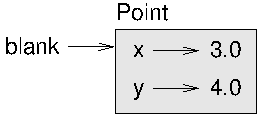
\includegraphics[scale=0.8]{figs/point.pdf}}
\caption{对象图.}
\label{fig.point}
\end{figure}

变量{\tt blank}指向了一个包含两个属性的Point对象. 
每个属性指向了一个浮点数. 

你可以基于同样语法, 读取属性值:

\begin{verbatim}
>>> blank.y
4.0
>>> x = blank.x
>>> x
3.0
\end{verbatim}
%
表达式{\tt blank.x}表示, ``定位{\tt blank}指向的对象, 获取{\tt x}的值.''
在上面例子中,  我们把这个表达式的值, 赋给了变量{\tt x}. 
变量{\tt x}和属性{\tt x}并不会出现冲突. 

同时, 你也可以在任意表达式中使用点标法. 比如:

\begin{verbatim}
>>> '(%g, %g)' % (blank.x, blank.y)
'(3.0, 4.0)'
>>> distance = math.sqrt(blank.x**2 + blank.y**2)
>>> distance
5.0
\end{verbatim}
%
你也可以将实例作为参数使用. 比如:
\index{instance!as argument}

\begin{verbatim}
def print_point(p):
    print('(%g, %g)' % (p.x, p.y))
\end{verbatim}
%
\verb"print_point"会接收一个点对象作为参数, 并用数学符号来表示. 
若要调用, 可以将{\tt blank}作为参数传入:

\begin{verbatim}
>>> print_point(blank)
(3.0, 4.0)
\end{verbatim}
%
在函数内部, {\tt p}是{\tt blank}的别称, 所以如果函数改变了{\tt p}, 
那么{\tt blank}也会发生变化. 
\index{aliasing}

做个练习, 写个\verb"distance_between_points"函数, 
使其接收两个Point对象作为参数, 返回两者之间的距离. 



\section{矩形}
\label{rectangles}

有时设置对象的属性很容易, 有时又很困难. 
假如你要设计一个类来表示矩形. 你会选择什么属性来描述位置和大小?
暂时忽略角度, 假设矩形要么垂直要么水平, 从而简化问题. 
\index{representation}

有两种方案可选: 

\begin{itemize}

\item 你可以确定矩形的一个角(或者中心, 以及宽度和高度. 

\item 你也可以声明两个对角的位置. 

\end{itemize}

现在很难说哪种更优, 我们先实现第一种方案, 做个示例. 
\index{Rectangle class}
\index{class!Rectangle}

下面是类定义:

\begin{verbatim}
class Rectangle:
    """Represents a rectangle. 

    attributes: width, height, corner.
    """
\end{verbatim}
%
文档字符串描述了相关属性: {\tt width}和
{\tt height}是数字; {\tt corner} 是个Point对象, 表示左下角位置. 

要表示一个矩形, 首先要初始化一个Rectangle对象, 并给属性赋值:

\begin{verbatim}
box = Rectangle()
box.width = 100.0
box.height = 200.0
box.corner = Point()
box.corner.x = 0.0
box.corner.y = 0.0
\end{verbatim}
%

表达式 {\tt box.corner.x}表示, 
``到{\tt box}指向的对象中, 选取名为{\tt corner}的属性;
然后再到{\tt corner}指向对象中, 选取名为{\tt x}的属性.''

\begin{figure}
\centerline
{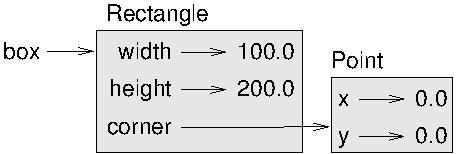
\includegraphics[scale=0.8]{figs/rectangle.pdf}}
\caption{对象图.}
\label{fig.rectangle}
\end{figure}


图~\ref{fig.rectangle} 展示了这个对象的状态图. 
一个对象作为另一个对象的属性存在, 叫做{\bf 嵌套}. 
\index{state diagram}
\index{diagram!state}
\index{object diagram}
\index{diagram!object}
\index{embedded object}
\index{object!embedded}


\section{返回实例}
\index{instance!as return value}
\index{return value}

函数也可以返回实例. 比如, \verb"find_center" 可以接收一个
 {\tt Rectangle}参数, 返回一个包含{\tt Rectangle}的中心位置坐标的{\tt Point}实例:

\begin{verbatim}
def find_center(rect):
    p = Point()
    p.x = rect.corner.x + rect.width/2
    p.y = rect.corner.y + rect.height/2
    return p
\end{verbatim}
%
下面的例子中, 传入了一个{\tt box}参数, 
然后将结果赋值给了{\tt center}变量:

\begin{verbatim}
>>> center = find_center(box)
>>> print_point(center)
(50, 100)
\end{verbatim}
%

\section{对象可变}
\index{object!mutable}
\index{mutability}

通过对属性赋值, 可以改变对象的状态. 
比如, 若要只改变矩形大小而不改变其位置, 可以只修改{\tt
width}和{\tt height}的值:

\begin{verbatim}
box.width = box.width + 50
box.height = box.height + 100
\end{verbatim}
%
你也可以通过函数, 修改对象. 例如, 
\verb"grow_rectangle" 函数会接收一个矩形对象和两个数值, 
{\tt dwidth}和{\tt dheight}, 然后分别累加到矩形的宽和高上:

\begin{verbatim}
def grow_rectangle(rect, dwidth, dheight):
    rect.width += dwidth
    rect.height += dheight
\end{verbatim}
%
下面展示了其使用效果:

\begin{verbatim}
>>> box.width, box.height
(150.0, 300.0)
>>> grow_rectangle(box, 50, 100)
>>> box.width, box.height
(200.0, 400.0)
\end{verbatim}
%
在函数内部, {\tt rect}是{\tt box}的别名, 所以当函数修改了{\tt rect}的属性, 
{\tt box}也会发生变化. 

做个练习, 编写\verb"move_rectangle"函数, 使其接收一个矩形对象以及
{\tt dx}和{\tt dy}两个值. 
同时对{\tt corner}的{\tt x}坐标加{\tt dx}, 
对{\tt corner}的{\tt y}坐标加上{\tt dy}, 
从而改变矩形的位置. 


\section{复制}
\label{copying}
\index{aliasing}

别名的使用会让程序变得复杂, 因为一处改动可能会影响到其他地方. 
同时, 追踪指向某个既定对象的所有变量, 又很困难. 
\index{copying objects}
\index{object!copying}
\index{copy module}
\index{module!copy}

所以, 常常用复制对象来代替别名使用. 
{\tt copy}模块包含一个{\tt copy}函数, 可以复制任意对象:

\begin{verbatim}
>>> p1 = Point()
>>> p1.x = 3.0
>>> p1.y = 4.0

>>> import copy
>>> p2 = copy.copy(p1)
\end{verbatim}
%
{\tt p1}和{\tt p2}包含同样的数据, 但它们不是同一个{\tt Point}对象.

\begin{verbatim}
>>> print_point(p1)
(3, 4)
>>> print_point(p2)
(3, 4)
>>> p1 is p2
False
>>> p1 == p2
False
\end{verbatim}
%

{\tt is}运算符表明{\tt p1}和{\tt p2}不是同一个对象, 这符合我们的预期. 
对于{\tt ==}, 本来我们看两者包含数据一样, 预期会是{\tt True}. 
但在此处, 令你沮丧的是, 对于实例来说, {\tt ==}运算符的默认操作和
{\tt is}运算符是一样的; 都是检验对象是否相同, 而不是判断是否相等.
这是因为对于用户自定义类型, Python至少现在还无法知道如何衡量相等.
\index{is operator}
\index{operator!is}
\index{identity}
\index{equivalence}

如果你用 {\tt copy.copy}来复制一个矩形, 
会发现只复制了{\tt Rectangle}对象, 并没有复制内嵌的{\tt Point}对象.
\index{embedded object!copying}

\begin{verbatim}
>>> box2 = copy.copy(box)
>>> box2 is box
False
>>> box2.corner is box.corner
True
\end{verbatim}

\begin{figure}
\centerline
{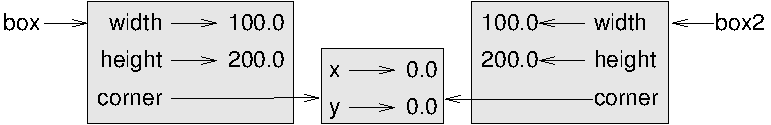
\includegraphics[scale=0.8]{figs/rectangle2.pdf}}
\caption{对象图.}
\label{fig.rectangle2}
\end{figure}

图~\ref{fig.rectangle2}展示了上面程序的对象图.
\index{state diagram}
\index{diagram!state}
\index{object diagram}
\index{diagram!object}
这种操作叫做{\bf 浅拷贝}, 因为仅仅复制对象和其内部引用, 而不会复制内嵌对象. 
\index{shallow copy}
\index{copy!shallow}

多数应用中, 我们所希望的并不是这个效果. 
在这个例子中, 对其中一个执行 \verb"grow_rectangle" 函数操作, 
并不会影响另一个, 但对任何一个调用 \verb"move_rectangle"函数, 两者都会被影响!
这种行为令人迷惑, 也更容易使人犯错. 
\index{deep copy}
\index{copy!deep}

幸运的是,  {\tt copy} 模块提供了一个{\tt
deepcopy}方法, 不仅复制对象, 同时也会复制其引用的对象, 
以及其引用对象内部引用的对象, 等等. 
所以, 你可以毫不意外地称其为{\bf 深拷贝}. 
\index{deepcopy function}
\index{function!deepcopy}

\begin{verbatim}
>>> box3 = copy.deepcopy(box)
>>> box3 is box
False
>>> box3.corner is box.corner
False
\end{verbatim}
%
{\tt box3}和{\tt box} 是完全隔离的对象了. 

做个练习, 编写一个 \verb"move_rectangle"新版本, 
使其创建并返回新的矩形对象, 而不是修改传入的对象. 

\section{调试}
\label{hasattr}
\index{debugging}

当你开始使用对象时, 极有可能遇到新的异常. 
如果试图读取一个不存在的属性, 会遇到属性异常{\tt AttributeError}:
\index{exception!AttributeError}
\index{AttributeError}

\begin{verbatim}
>>> p = Point()
>>> p.x = 3
>>> p.y = 4
>>> p.z
AttributeError: Point instance has no attribute 'z'
\end{verbatim}
%
如若不确定对象类型, 可以如下这般查看:
\index{type function}
\index{function!type}

\begin{verbatim}
>>> type(p)
<class '__main__.Point'>
\end{verbatim}
%
你也可以使用{\tt isinstance}来判断对象是否是某个类的实例:
\index{isinstance function}
\index{function!isinstance}

\begin{verbatim}
>>> isinstance(p, Point)
True
\end{verbatim}
%
如果你不确定对象是否存在某个属性, 
可以用内置函数{\tt hasattr}, 进行判断:
\index{hasattr function}
\index{function!hasattr}

\begin{verbatim}
>>> hasattr(p, 'x')
True
>>> hasattr(p, 'z')
False
\end{verbatim}
%
第一个参数可以是任意对象;
第二参数是个{\em 字符串}, 也就是某个属性的名称. 
\index{attribute}

你也可以用{\tt try}语句, 来判断对象是否具有你所要的属性:
\index{try statement}
\index{statement!try}

\begin{verbatim}
try:
    x = p.x
except AttributeError:
    x = 0
\end{verbatim}

这种方法便于编写适用不同情况的函数;
更多相关话题在第~\ref{polymorphism}节会详述. 


\section{术语表}

\begin{description}

\item[类(class):] 用户自定义类型. 一个类的声明会创建一个新的类对象. 
\index{class}
\index{programmer-defined type}
\index{type!programmer-defined}

\item[类对象(class object):] 包含自定义类型信息的对象. 
类对象可用来创建类的实例. 
\index{class object}
\index{object!class}

\item[实例(instance):] 属于某个类的对象. 
\index{instance}

\item[初始化(instantiate):] 创建一个新对象.
\index{instantiate}

\item[属性(attribute):] 一种与对象关联的命名值. 
\index{attribute!instance}
\index{instance attribute}

\item[内嵌对象(embedded object):] 作为属性存在于另一个对象内的对象. 
\index{embedded object}
\index{object!embedded}

\item[浅拷贝(shallow copy):] 复制对象的内容, 以及内嵌对象的所有引用;
通过{\tt copy}模块中的{\tt copy}函数实现. 
\index{shallow copy}

\item[深拷贝(deep copy):] 复制对象内容以及所有内嵌对象, 以及内嵌对象的内嵌对象, 等等;
通过{\tt copy} 模块的{\tt deepcopy}函数实现. 
\index{deep copy}

\item[对象图(object diagram):] 展示对象, 及其属性, 和属性值的图. 
\index{object diagram}
\index{diagram!object}

\end{description}


\section{习题集}

\begin{exercise}

定义一个名为 {\tt Circle}的类, 包含属性{\tt center}和{\tt radius}, 
 {\tt center}是一个Point对象, {\tt radius}是一个数字. 

初始化一个{\tt Circle}对象, 用来表示一个圆, 其圆心为$(150, 100)$, 
半径为 75.

编写\verb"point_in_circle" 函数, 以Circle和Point为入参, 
如果Point 在圆内或者圆周上, 则返回True. 

编写\verb"rect_in_circle"函数, 传入一个Circle和一个Rectangle, 
如果Rectangle 完全处于圆内或圆周上, 则返回True. 

编写函数\verb"rect_circle_overlap", 接收一个Circle和一个Rectangle, 
如果Rectangle的任意一个顶点在圆内, 则返回True. 
或者写个更有挑战性的版本, 如果矩形有任意部分在圆内, 则返回True. 

参考答案: \url{http://thinkpython2.com/code/Circle.py}.

\end{exercise}


\begin{exercise}

编写函数\verb"draw_rect", 接收一个Turtle对象和一个Rectangle, 
用Turtle 绘制Rectangle. 
可以参考第~\ref{turtlechap}节的Turtle对象的使用示例. 

编写函数\verb"draw_circle",  接收一个Turtle对象和一个Circle对象, 并绘制Circle.


参考答案: \url{http://thinkpython2.com/code/draw.py}.

\end{exercise}



\chapter{类和函数}
\label{time}

目前, 我们已经知道了如何创建新的类型, 下一步, 我们学习如何用
自定义类型对象作为参数和返回值, 编写函数. 
本章将介绍``函数式编程模式'', 以及两种新的程序开发范式. 


本章的代码样例可以从\url{http://thinkpython2.com/code/Time1.py}下载. 
习题答案可以参考
\url{http://thinkpython2.com/code/Time1_soln.py}.


\section{时间}
\label{isafter}

下面是一个自定义类型的示例, 我们定义了一个{\tt Time}类, 
用来记录一天的时间. 
类的定义如下: 
\index{programmer-defined type}
\index{type!programmer-defined} 
\index{Time class} \index{class!Time}

\begin{verbatim}
class Time:
    """Represents the time of day.
       
    attributes: hour, minute, second
    """
\end{verbatim}
%
我们可以创建一个新的{\tt Time}对象, 
对时分秒分别定义属性并赋值:

\begin{verbatim}
time = Time()
time.hour = 11
time.minute = 59
time.second = 30
\end{verbatim}
%
{\tt Time}对象的状态图如图~\ref{fig.time}所示.
\index{state diagram}
\index{diagram!state}
\index{object diagram}
\index{diagram!object}

做个练习, 编写\verb"print_time"函数, 令其接收一个Time对象, 并按照
{\tt 时:分:秒}的格式输出. 
提示: 格式序列 \verb"'%.2d'"会
用至少两位输出整数, 不足两位则前面补0. 

编写一个名为 \verb"is_after"的布尔函数, 
令其接收两个Time对象, {\tt t1}和{\tt t2}, 
如果{\tt t1}晚于{\tt t2}, 则返回{\tt True}, 否则返回{\tt False}. 
挑战之处: 不要用{\tt if}语句. 

\begin{figure}
\centerline
{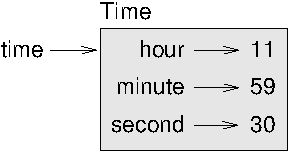
\includegraphics[scale=0.8]{figs/time.pdf}}
\caption{对象图.}
\label{fig.time}
\end{figure}


\section{纯函数}
\index{prototype and patch}
\index{development plan!prototype and patch}

下面章节中, 我们将编写两个函数, 实现时间计算. 
这两个函数展示了两种函数类型: 纯函数以及修改器. 
同时, 也展示了一个我称之为{\tt 原型和补丁}的开发范式, 
这是一种通过构建简单原型, 逐步改进, 从而解决复杂问题的方法. 

以下为 \verb"add_time"的一个简单原型:

\begin{verbatim}
def add_time(t1, t2):
    sum = Time()
    sum.hour = t1.hour + t2.hour
    sum.minute = t1.minute + t2.minute
    sum.second = t1.second + t2.second
    return sum
\end{verbatim}
%
该函数新建了一个{\tt Time}对象, 并初始化其属性, 同时返回对象的引用. 
这便称之为{\tt 纯函数}, 因为它不会修改作为参数传入的任何对象, 
同时也不会产生其他效果, 比如显示值或提示用户输入, 而仅仅是返回一个值. 
\index{pure function}
\index{function type!pure}

为了测试此函数, 新建两个Time对象: 包含某电影开始时间的{\tt start}, 
比如电影{\em Monty Python and the Holy Grail},  
以及放映时长的{\tt duration}, 此处时长为1小时35分钟. 
\index{Monty Python and the Holy Grail}

\verb"add_time" 会计算出电影结束时间. 

\begin{verbatim}
>>> start = Time()
>>> start.hour = 9
>>> start.minute = 45
>>> start.second =  0

>>> duration = Time()
>>> duration.hour = 1
>>> duration.minute = 35
>>> duration.second = 0

>>> done = add_time(start, duration)
>>> print_time(done)
10:80:00
\end{verbatim}
%
结果值{\tt 10:80:00}, 肯定不是你想要的. 
问题在于, 函数没有处理秒数或分钟数相加后超过60的情况. 
遇到这种情况, 我们需要将每60秒进位到分钟, 
每60分钟进位到小时. 
\index{carrying, addition with}

优化后的版本如下:

\begin{verbatim}
def add_time(t1, t2):
    sum = Time()
    sum.hour = t1.hour + t2.hour
    sum.minute = t1.minute + t2.minute
    sum.second = t1.second + t2.second

    if sum.second >= 60:
        sum.second -= 60
        sum.minute += 1

    if sum.minute >= 60:
        sum.minute -= 60
        sum.hour += 1

    return sum
\end{verbatim}
%
这个函数虽然正确, 但是略显臃肿. 
稍后我们将看到一个简短版本. 


\section{修改器}
\label{increment}
\index{modifier}
\index{function type!modifier}

有时, 对于一个函数来说, 直接修改其获取的参数对象, 更为高效. 
在此情境中, 更改对于调用者来说, 是可见的. 
这样的函数, 被称之为{\bf 修改器}. 
\index{increment}

函数{\tt increment}, 是对{\tt Time}对象增加特定秒数, 
这天然便适合用修改器实现. 
下面是个初稿:

\begin{verbatim}
def increment(time, seconds):
    time.second += seconds

    if time.second >= 60:
        time.second -= 60
        time.minute += 1

    if time.minute >= 60:
        time.minute -= 60
        time.hour += 1
\end{verbatim}
%
第一行执行基本操作;
其余的则处理我们之前看到的特殊情况. 
\index{special case}

这个函数正确吗? 如果{\tt seconds}远大于60, 会怎样?

这时, 只进位一次是不够的;
我们需要重复执行, 直到{\tt time.second}小于60.
一种解决方案是用{\tt while}语句替换{\tt if}语句. 
虽然可行, 但不够高效. 
做个练习, 编写一个不包含任何循环的{\tt increment}正确版本. 

修改器所为, 纯函数皆可为. 
事实上, 有些编程语言只允许使用纯函数. 
有证据表明, 使用纯函数比使用修改器, 开发更快, 出错更少. 
但有时修改器用来更方便, 而函数式程序则效率不高. 

通常, 我建议在合理的情况下, 都使用纯函数, 只有在优势明显时才
采用修改器. 这种方法便称之为{\bf 函数式编程模式}. 
\index{functional programming style}

做个练习, 编写一个``纯''版本的{\tt increment}函数, 使其创建并返回新的Time对象, 
而不是修改其参数. 


\section{原型与规划}
\label{prototype}
\index{prototype and patch}
\index{development plan!prototype and patch}
\index{planned development}
\index{development plan!designed}

刚刚展示的开发方案是``原型和补丁''.
就是针对每个函数, 编写一个可以完成基本运算的原型, 然后对其测试, 
并逐步修正错误. 

这种方法很有效, 尤其在你尚未对问题有深入了解时. 
但是增量修正往往会产生大量过于复杂代码---因为需要关注特殊情况---和不可靠的代码
---因为你很难确定是否找到了所有异常. 

另一种方法是采用{\bf 设计开发}, 用这种方法, 就是采用上帝视角处理问题, 
从而开发会容易很多. 
在这里, 这个视角就是Time对象, 实际是三个六十进制的数字(参考\url{http://en.wikipedia.org/wiki/Sexagesimal}). 
{\tt second}属性是``个位'', {\tt minute}属性是``60位'', {\tt hour}属性是``3600位''.
\index{sexagesimal}

当我们编写\verb"add_time" 和{\tt increment}函数时, 
实际是进行60位的加法, 着就是为何我们需要从当前位进位到下一位的原因. 
\index{carrying, addition with}

这个发现给出了另一种解决问题的方法---我们将Time对象转为整数, 
然后利用计算机善于进行整数运算的优势. 

这是个将Time对象转为整数的函数:

\begin{verbatim}
def time_to_int(time):
    minutes = time.hour * 60 + time.minute
    seconds = minutes * 60 + time.second
    return seconds
\end{verbatim}
%
下面函数可以将整数转换为Time(回忆一下{\tt divmod}, 也就是将第一个参数除以第二个参数, 
将商和余数作为元组返回). 
\index{divmod}

\begin{verbatim}
def int_to_time(seconds):
    time = Time()
    minutes, time.second = divmod(seconds, 60)
    time.hour, time.minute = divmod(minutes, 60)
    return time
\end{verbatim}
%
你可能需要费点脑力, 并运行一些测试, 以说服自己这些函数是正确的. 
一种方法是针对各种{\tt x}值, 检查\verb"time_to_int(int_to_time(x)) == x"是否正确. 
这就是一种一致性检验. 
\index{consistency check}

一旦你确信它们正确, 便可以用其重写\verb"add_time":

\begin{verbatim}
def add_time(t1, t2):
    seconds = time_to_int(t1) + time_to_int(t2)
    return int_to_time(seconds)
\end{verbatim}
%
这个版本相比原来的版本, 更容易验证. 
试一下, 用\verb"time_to_int" 和
\verb"int_to_time"来重写{\tt increment} . 

在某些方面, 60进制与10进制的相互转换相比时间处理要更难. 
因为进制转换更加抽象;
而时间处理更符合我们的直观感受. 

但如果我们注意到时间不过是60进制的数字, 并预先编写转换函数 (\verb"time_to_int"
和 \verb"int_to_time"), 便可以得到一个更精简, 易读, 易调试, 也更可靠的程序. 

同时这也更利于后续添加新的功能. 
比如, 假如要对两个Time对象相减, 获取其时间间隔. 
直接的方法, 便是通过借位实现. 
但是, 使用转换函数, 会更容易, 也更可能正确. 
\index{subtraction with borrowing}
\index{borrowing, subtraction with}
\index{generalization}

讽刺的是, 有时候将问题想得复杂(或更通用), 反而会更容易解决(因为特殊情况会更少, 
出错概率也会更低).


\section{调试}
\index{debugging}

如果{\tt minute}和{\tt second}在0到60之间(包括0但不包括60),
同时{\tt hour}是正数, 那这个Time对象便是正确的. 
{\tt hour}和{\tt minute}应该是整数, 但{\tt second}可以允许有小数部分. 
\index{invariant}

这种约束条件, 叫做{\bf 不变式}, 因为它们需要恒为真. 
换句话说, 如果它们不是真, 那肯定有某些地方出错了. 

编写代码来检查不变式, 可以帮助发现错误并找出原因. 
比如, 你可能有个函数\verb"valid_time" , 它会接收一个Time对象, 
如果违反了不变式的某个条件, 返回{\tt False}:

\begin{verbatim}
def valid_time(time):
    if time.hour < 0 or time.minute < 0 or time.second < 0:
        return False
    if time.minute >= 60 or time.second >= 60:
        return False
    return True
\end{verbatim}
%
在每个函数的开始部分, 你都可以检查参数并确保它们合法:
\index{raise statement}
\index{statement!raise}

\begin{verbatim}
def add_time(t1, t2):
    if not valid_time(t1) or not valid_time(t2):
        raise ValueError('invalid Time object in add_time')
    seconds = time_to_int(t1) + time_to_int(t2)
    return int_to_time(seconds)
\end{verbatim}
%
或者你也可以用{\bf assert 语句}, 检查一个给定的不变式, 如果失败, 抛出异常:
\index{assert statement}
\index{statement!assert}

\begin{verbatim}
def add_time(t1, t2):
    assert valid_time(t1) and valid_time(t2)
    seconds = time_to_int(t1) + time_to_int(t2)
    return int_to_time(seconds)
\end{verbatim}
%
{\tt assert}语句非常有用, 因为它们区分了何为常规条件代码, 何为检验错误的代码. 


\section{术语表}

\begin{description}

\item[原型和补丁(prototype and patch):] 一种通过先写程序初稿, 然后测试, 并修正发现的错误的开发方案. 
\index{prototype and patch}

\item[设计开发(designed development):] 一种开发方案, 采用上帝视角处理问题, 
相比于增量开发或者原型开发, 需要更多提前规划. 
\index{designed development}

\item[纯函数(pure function):] 一种不修改任何作为参数传入的对象的函数. 
多数纯函数有返回值. 
\index{pure function}

\item[修改器(modifier):] 一种函数, 
会修改作为参数接收的一个或者多个对象. 
多数修改器都是没有返回值的;
也就是说, 它们返回{\tt None}. \index{modifier}

\item[函数式编程风格(functional programming style):] 一种程序设计风格, 其中多数函数
都是纯函数.
\index{functional programming style}

\item[不变式(invariant):] 程序执行期间, 应该始终为真的条件. 
\index{invariant}

\item[断言语句(assert statement):] 检查条件是否满足, 并在失败时抛出异常的语句. 
\index{assert statement}
\index{statement!assert}

\end{description}


\section{习题集}

本章代码样例在
\url{http://thinkpython2.com/code/Time1.py}; 
同时习题答案在\url{http://thinkpython2.com/code/Time1_soln.py}.

\begin{exercise}

编写\verb"mul_time" 函数, 接收一个Time对象以及一个数字, 
返回一个原始时间和数字的乘积的新时间对象. 

然后用\verb"mul_time" 来编写一个函数, 接收一个表示比赛结束时间的Time对象, 
以及一个表示距离的数字, 返回一个表示平均配速(每英里耗时)的Time对象. 
\index{running pace}

\end{exercise}


\begin{exercise}
\index{datetime module}
\index{module!datetime}

{\tt datetime}模块提供的{\tt time}对象和本章的Time对象相似, 
但是前者提供了更丰富的方法和操作. 
可在\url{http://docs.python.org/3/library/datetime.html}阅读相关文档.

\begin{enumerate}

\item 使用 {\tt datetime} 模块编写程序, 获取当前日期并打印星期几. 

\item 编写个程序, 输入生日, 输出用户的年龄以及距离下个生日的
天数, 小时数, 分钟数和秒数. 
\index{birthday}

\item 对于两个生日不同的人, 
总有一天, 一个人的出生天数是另一个人的两倍. 
我们称之为``双倍日''.
编写个程序, 输入两个生日, 计算他们的``双倍日''.

\item 进阶一下, 编写个更通用的版本, 计算某人的出生天数是另一个$n$倍大的那一天. 
\index{Double Day}

\end{enumerate}

参看: \url{http://thinkpython2.com/code/double.py}

\end{exercise}


\chapter{类和方法}

虽然我们已经接触了一些Python的面向对象的特性, 
但前面两章的内容并不算是真正的面向对象, 
因为自定义类型与操作它们的函数之间的关系, 并未涉及. 
下面会将这些函数转换为方法, 从而使其关系明晰. 

本章代码可以从
\url{http://thinkpython2.com/code/Time2.py}下载, 
同时习题答案在\url{http://thinkpython2.com/code/Point2_soln.py}中.


\section{面向对象特性}
\index{object-oriented programming}

Python是个{\bf 面向对象编程语言}, 
也就是说, 它提供了支持面向对象编程的诸多特性, 而面向对象编程有以下特征:

\begin{itemize}

\item 程序包括类和方法定义.

\item 多数运算都基于对象操作而存在. 

\item 对象通常表示现实世界中的事物, 方法通常对应现实世界中事物的交互方式. 

\end{itemize}

比如, 在第~\ref{time}节定义的{\tt Time}类, 对应人们记录一天中时间的方式, 
而我们定义的函数, 则对应了人们处理时间的不同策略. 
类似的, 第~\ref{clobjects}节的{\tt Point}和{\tt Rectangle}类, 
分别表示点和矩形的数学概念. 

到目前为止, 我们都还没有充分使用Python提供的支持面向对象编程的强大功能. 
这些功能严格来说并非必须;
多数功能的语法我们都已经变相实现过了. 
但很多时候, 面向对象的语法更加简洁, 同时更加精确地表达程序结构. 

比如, 在{\tt Time1.py}中, 类定义和函数定义并无明显关联. 
认真观察, 便会发现每个函数都至少有一个{\tt Time}对象作为参数. 
\index{method}
\index{function}

透过观察, 很自然地引出了{\bf 方法};
一个方法便是一个与某个类相关联的函数. 
我们已经接触过字符串, 列表, 字典和元组的方法. 
本章中, 我们将构建自定义类型的方法. 
\index{syntax}
\index{semantics}
\index{programmer-defined type}
\index{type!programmer-defined}

方法和函数, 语义相同, 但语法有两处差异:

\begin{itemize}

\item 方法定义在类中, 以使类和方法的关系一目了然. 

\item 调用方法的语法和调用函数的语法不同. 

\end{itemize}

后面章节中, 我们将把前两章涉及的函数转换为方法. 
这种转换纯粹是机械性的; 通过一系列步骤便可实现. 
如果你可以熟练地从一种形式转换为另一种形式, 
那么你便能够为眼下的事情, 选择最合适的形式. 

\section{打印对象}
\index{object!printing}

在第~\ref{time}节, 我们定义了{\tt Time}类, 在第~\ref{isafter}节, 
你编写了\verb"print_time"函数:

\begin{verbatim}
class Time:
    """Represents the time of day."""

def print_time(time):
    print('%.2d:%.2d:%.2d' % (time.hour, time.minute, time.second))
\end{verbatim}
%
若要调用函数, 需要传递一个{\tt Time}对象作为参数:

\begin{verbatim}
>>> start = Time()
>>> start.hour = 9
>>> start.minute = 45
>>> start.second = 00
>>> print_time(start)
09:45:00
\end{verbatim}
%

要使\verb"print_time" 成为方法, 只需要将函数定义移动到类定义内部. 
同时注意缩进的变化. 
\index{indentation}

\begin{verbatim}
class Time:
    def print_time(time):
        print('%.2d:%.2d:%.2d' % (time.hour, time.minute, time.second))
\end{verbatim}
%
现在有两种方式调用\verb"print_time" . 
第一种(也是不常用的)方式是使用函数语法:
\index{function syntax}
\index{dot notation}

\begin{verbatim}
>>> Time.print_time(start)
09:45:00
\end{verbatim}
%
这里用到了点标法, {\tt Time}是类的名称, 
\verb"print_time"是方法的名称. 
{\tt start}是传入的参数. 

第二种(也是更简洁的)方式, 是使用方法语法:
\index{method syntax}

\begin{verbatim}
>>> start.print_time()
09:45:00
\end{verbatim}
%
这里也用了点标法, \verb"print_time" 也是方法的名字, {\tt start}是调用方法的对象, 
也被称为{\tt 主体}. 
正如句子的主语是句子主体, 方法的调用主体也就是方法的主体. 
\index{subject}

在方法内部, 主体被赋值给了第一个参数, 所以在这里{\tt start}被赋值给了{\tt time}.
\index{self (parameter name)}
\index{parameter!self}

按照惯例, 方法的第一个参数称为{\tt self}, 所以\verb"print_time"的常见写法如下:

\begin{verbatim}
class Time:
    def print_time(self):
        print('%.2d:%.2d:%.2d' % (self.hour, self.minute, self.second))
\end{verbatim}
%

这种约定是有其内在缘由的:
\index{metaphor, method invocation}

\begin{itemize}

\item 函数调用的语法, \verb"print_time(start)",  表示函数是主动一方. 
就像, ``嘿, \verb"print_time"!  这有个对象需要你打印一下.''

\item 在面向对象编程中, 对象是主动一方. 像\verb"start.print_time()"这种方法调用, 
就像是说, ``嗨, {\tt start}! 请打印你自己. ''

\end{itemize}

这种视角的转换看似更优雅了, 但并没有明显的优势. 
在目前遇到的例子中, 看不出什么差异. 
但有时候, 将触发者从函数转移到对象上, 
可以写出更通用的函数(或方法), 便于后期维护和复用. 

做个练习, 将\verb"time_to_int"(见第~\ref{prototype}节), 重写为方法. 
你可以尝试将\verb"int_to_time" 也重写为方法, 但没有什么意义, 
因为没有对象可以调用它. 


\section{另一个示例}
\index{increment}

下面是 {\tt increment}(章节~\ref{increment})作为方法的重写版本:

\begin{verbatim}
# inside class Time:

    def increment(self, seconds):
        seconds += self.time_to_int()
        return int_to_time(seconds)
\end{verbatim}
%
这个版本假设 \verb"time_to_int" 已经被重写为了方法. 
同时, 也要注意它是一个纯函数, 而不是修改器. 

下面是调用{\tt increment}的方式:

\begin{verbatim}
>>> start.print_time()
09:45:00
>>> end = start.increment(1337)
>>> end.print_time()
10:07:17
\end{verbatim}
%
主体{\tt start}, 被赋值给了第一个参数{\tt self}. 
实参{\tt 1337}, 则被分配给了第二个参数, {\tt seconds}. 

这种机制让人感觉很迷惑, 尤其是产生错误的时候. 
比如, 如果你用两个实参调用{\tt increment}, 会报错:
\index{exception!TypeError}
\index{TypeError}

\begin{verbatim}
>>> end = start.increment(1337, 460)
TypeError: increment() takes 2 positional arguments but 3 were given
\end{verbatim}
%
这个错误信息初看很难理解, 因为括号里只有两个参数. 
但这个主体也被当作了一个参数, 所以一共有三个. 

另外, {\bf 位置参数}是没有参数名的参数;
也就是说, 它不是关键字参数. 
下面函数调用中:
\index{positional argument}
\index{argument!positional}

\begin{verbatim}
sketch(parrot, cage, dead=True)
\end{verbatim}

{\tt parrot}和{\tt cage}是位置参数, 而{\tt dead}是
关键字参数.


\section{一个进阶案例}

重写\verb"is_after"(见第~\ref{isafter}节)会略微复杂, 因为它需要两个Time对象作为参数. 
这种情况, 通常将第一个参数命名为{\tt self}, 第二个命名为{\tt other}:
\index{other (parameter name)}
\index{parameter!other}

\begin{verbatim}
# inside class Time:

    def is_after(self, other):
        return self.time_to_int() > other.time_to_int()
\end{verbatim}
%
若要使用此方法, 你需要在某个对象上调用此方法, 并将另一个对象作为参数传入:

\begin{verbatim}
>>> end.is_after(start)
True
\end{verbatim}
%
这种语法的一个好处, 是它读起来如同英语: ``end is after start?''


\section{init方法}
\index{init method}
\index{method!init}

init方法(``initialization''的简称)是一个特殊的方法, 
在对象被实例化时才被调用. 
其全称为\verb"__init__"(两个下划线, 然后紧跟{\tt init}, 然后又是两个下划线).
{\tt Time}类的init方法如下:

\begin{verbatim}
# inside class Time:

    def __init__(self, hour=0, minute=0, second=0):
        self.hour = hour
        self.minute = minute
        self.second = second
\end{verbatim}
%
通常\verb"__init__"方法的参数名称和类中属性名称相同. 
下面语句

\begin{verbatim}
        self.hour = hour
\end{verbatim}
%
会将参数{\tt hour}的值存储为{\tt self}的一个属性.
\index{optional parameter}
\index{parameter!optional}
\index{default value}
\index{override}

这个参数是可选的, 所以如果你调用{\tt Time}时没有传参, 
那便会使用默认值. 

\begin{verbatim}
>>> time = Time()
>>> time.print_time()
00:00:00
\end{verbatim}
%
如果你提供了一个参数, 那只会覆盖{\tt hour}:

\begin{verbatim}
>>> time = Time (9)
>>> time.print_time()
09:00:00
\end{verbatim}
%
如果提供了两个参数, 则会覆写{\tt hour}和{\tt minute}.

\begin{verbatim}
>>> time = Time(9, 45)
>>> time.print_time()
09:45:00
\end{verbatim}
%
如果提供三个参数, 则会覆写三个默认值. 

做个练习, 为{\tt Point}类编写init方法, 使用{\tt x}和 {\tt y} 作为可选参数, 
并赋值给相应的属性. 
\index{Point class}
\index{class!Point}


\section{{\tt \_\_str\_\_}方法}
\index{str method@\_\_str\_\_ method}
\index{method!\_\_str\_\_}

\verb"__str__" 和 \verb"__init__"类似, 也是一个特殊的方法, 
其一般返回对象的字符串表示. 
\index{string representation}

比如, 下面是Time对象的{\tt str}方法:

\begin{verbatim}
# inside class Time:

    def __str__(self):
        return '%.2d:%.2d:%.2d' % (self.hour, self.minute, self.second)
\end{verbatim}
%
当用{\tt print}打印对象时, Python调用的就是{\tt str}方法:
\index{print statement}
\index{statement!print}

\begin{verbatim}
>>> time = Time(9, 45)
>>> print(time)
09:45:00
\end{verbatim}
%
当编写新类时, 我总是先写\verb"__init__"方法, 这样更容易初始化对象, 
同时编写\verb"__str__"方法, 以方便调试. 

试着为{\tt Point}类编写{\tt str}方法. 
创建一个Point对象, 并打印输出. 


\section{运算符重载}
\label{operator.overloading}

通过定义一些特殊方法, 你可以对自定义类型, 重新定义运算符的行为. 
比如, 你为{\tt Time}类定义了\verb"__add__" 方法, 便可以用{\tt +}运算符操作Time对象. 
\index{programmer-defined type}
\index{type!programmer-defined}

如下定义:
\index{add method}
\index{method!add}

\begin{verbatim}
# inside class Time:

    def __add__(self, other):
        seconds = self.time_to_int() + other.time_to_int()
        return int_to_time(seconds)
\end{verbatim}
%
可以这样使用:

\begin{verbatim}
>>> start = Time(9, 45)
>>> duration = Time(1, 35)
>>> print(start + duration)
11:20:00
\end{verbatim}
%
当对Time对象应用{\tt +}运算符时, Python会调用\verb"__add__".
当打印结果时, Python会调用\verb"__str__".
所以我们看到的, 只是冰山一角而已!
\index{operator overloading}

对自定义类型, 改变运算符的行为, 这便是{\bf 运算符重载}. 
对于Python中的每个运算符, 都有一个类似\verb"__add__"的特殊方法与之对应. 
更多详细信息, 请参考
\url{http://docs.python.org/3/reference/datamodel.html#specialnames}.

作为练习, 请为Point类编写{\tt add}方法. 

\section{类型分发}

在上一节, 我们将两个Time对象进行加法操作, 
但是你可能想将一个整数与Time对象相加. 
下面是一个\verb"__add__"的新版本, 它会检验{\tt other}的类型, 
从而决定调用\verb"add_time" , 还是{\tt increment}方法:

\begin{verbatim}
# inside class Time:

    def __add__(self, other):
        if isinstance(other, Time):
            return self.add_time(other)
        else:
            return self.increment(other)

    def add_time(self, other):
        seconds = self.time_to_int() + other.time_to_int()
        return int_to_time(seconds)

    def increment(self, seconds):
        seconds += self.time_to_int()
        return int_to_time(seconds)
\end{verbatim}
%
内置函数{\tt isinstance}会接收一个值和一个类对象, 
如果值是这个类的实例, 则返回{\tt True}.
\index{isinstance function}
\index{function!isinstance}

如果{\tt other} 是一个Time对象, 
\verb"__add__"会调用\verb"add_time". 
否则, 会认为参数是个数字, 从而调用{\tt increment}方法. 
这种操作叫做{\tt 类型分发}, 因为它基于参数的类型不同, 
将计算任务分发给不同的方法. 
\index{type-based dispatch}
\index{dispatch, type-based}

下面时一个在不同类型上使用{\tt +}运算符的例子:

\begin{verbatim}
>>> start = Time(9, 45)
>>> duration = Time(1, 35)
>>> print(start + duration)
11:20:00
>>> print(start + 1337)
10:07:17
\end{verbatim}
%
不幸的是, 这个加法的实现并不具有可交换性. 
如果整数在前, 你会得到报错:
\index{commutativity}

\begin{verbatim}
>>> print(1337 + start)
TypeError: unsupported operand type(s) for +: 'int' and 'instance'
\end{verbatim}
%
问题在于, Python并不是对Time对象加上一个整数, 
而是对一个整数加上Time对象, 
所以不知道如何处理了. 
有个取巧的解决办法: 用特殊方法\verb"__radd__", 表示``右侧相加''. 
当Time对象出现在{\tt +}运算符右侧时, 将调用此方法. 
以下是定义:
\index{radd method}
\index{method!radd}

\begin{verbatim}
# inside class Time:

    def __radd__(self, other):
        return self.__add__(other)
\end{verbatim}
%
下面是使用方式:

\begin{verbatim}
>>> print(1337 + start)
10:07:17
\end{verbatim}
%

做个练习, 为Points编写{\tt add}方法, 使其同时适用于Point对象和元组:

\begin{itemize}

\item 如果第二个操作数是Point对象, 方法则返回一个新的Point, 
其$x$坐标是操作数的$x$坐标总和, $y$坐标同理. 

\item 如果第二个操作数是元组, 则方法应该将元组的第一个元素和$x$坐标相加, 
第二个元素和$y$坐标相加, 然后返回此结果的一个新Point对象. 

\end{itemize}


\section{多态性}
\label{polymorphism}

当需要的时候, 基于类型分发是有用的, 但(幸好)不用总要如此. 
通常, 你可以编写适用不同类型参数的函数, 来避免类型分发. 
\index{type-based dispatch}
\index{dispatch!type-based}

我们为字符串操作编写的很多函数, 对于其他序列类型也适用. 
比如, 在第~\ref{histogram}节, 我们用{\tt histogram} 来统计单词中每个字母出现的次数. 

\begin{verbatim}
def histogram(s):
    d = dict()
    for c in s:
        if c not in d:
            d[c] = 1
        else:
            d[c] = d[c]+1
    return d
\end{verbatim}
%
这个函数对于列表, 元组, 甚至字典都适用, 只要{\tt s}中的元素是可哈希的, 
就都可以作为{\tt d}的键. 

\begin{verbatim}
>>> t = ['spam', 'egg', 'spam', 'spam', 'bacon', 'spam']
>>> histogram(t)
{'bacon': 1, 'egg': 1, 'spam': 4}
\end{verbatim}
%
能够处理多种类型的函数, 称为{\bf 多态}. 
多态性有助于代码复用. 
例如, 可以对序列中元素求和的内置函数{\tt sum}, 
也同样适用于其他支持加法运算的元素序列. 
\index{polymorphism}

因为Time对象也提供了{\tt add}方法, 所以也同样适用于{\tt sum}:

\begin{verbatim}
>>> t1 = Time(7, 43)
>>> t2 = Time(7, 41)
>>> t3 = Time(7, 37)
>>> total = sum([t1, t2, t3])
>>> print(total)
23:01:00
\end{verbatim}
%
通常, 如果函数内的所有操作适用于某种类型, 那么这个函数便同样适用于此类型. 

最好的多态, 是那种不求而得, 
就像你突然发现你写的函数, 对于规划之外的某种类型, 也同样适用. 


\section{调试}
\index{debugging}

在程序运行的任何时刻, 向对象添加属性都是可行的, 
但如果对象类型相同, 属性不同, 那很容易出错. 
所以比较好的方法是在init方法中初始化对象的全部属性. 
\index{init method}
\index{attribute!initializing}

如果你不确定一个对象是否包含某个属性, 可以适用内置函数{\tt hasattr}
 (见第~\ref{hasattr}节)进行判断. 
\index{hasattr function}
\index{function!hasattr}
\index{dict attribute@\_\_dict\_\_ attribute}
\index{attribute!\_\_dict\_\_}

另一种获取属性的方式, 是使用内置函数{\tt vars},
它会接收一个对象, 并返回一个属性名(字符串格式)映射到属性值的字典:

\begin{verbatim}
>>> p = Point(3, 4)
>>> vars(p)
{'y': 4, 'x': 3}
\end{verbatim}
%

对于调试而言, 你会发现保留下面的函数, 会很有用:

\begin{verbatim}
def print_attributes(obj):
    for attr in vars(obj):
        print(attr, getattr(obj, attr))
\end{verbatim}
%
\verb"print_attributes"会遍历字典, 输出每个属性名称以及其对应的值. 
\index{traversal!dictionary}
\index{dictionary!traversal}

内置函数{\tt getattr}会接收一个对象和一个属性名(字符串格式), 返回该属性的值. 
\index{getattr function}
\index{function!getattr}


\section{接口和实现}

面向对象设计的一个目标便是令软件便于维护, 
也就是说当系统的某些部分发生了变化, 你依然可以保证程序正常运行, 
从而可以修改程序, 以满足新的需求. 
\index{interface}
\index{implementation}
\index{maintainable}
\index{object-oriented design}

实现这一目标的一个设计原则便是, 接口和实现分离. 
对于对象来说, 就是类提供的方法不应该依赖于属性的形式. 
\index{attribute}

比如, 本章我们开发了一个类, 表示一天中某个时间. 
这个类提供的方法包括
\verb"time_to_int", \verb"is_after", 以及\verb"add_time".

我们有多种方式实现这些方法. 
实现的细节取决于我们如何表示时间. 
在本章, {\tt Time}对象的属性有{\tt hour}, {\tt minute}, 和
{\tt second}. 

同样的, 我们也可以用一个整数, 即从零点以来的秒数来表示这些属性. 
这种实现方式, 将会令某些方法, 比如\verb"is_after", 更容易实现, 而令某些方法更难编写. 

当你应用了一个新的类后, 你可能发现更好的实现方式. 
但如果程序的其他部分正在使用你的类, 这时候修改接口, 
往往比较耗时, 且容易出错. 

但如果你设计接口时足够仔细, 你便可以在不改变接口的同时, 修改内部实现, 
也就意味着程序其他部分无需变动. 


\section{术语表}

\begin{description}

\item[面向对象语言(object-oriented language):] 提供自定义类型和方法等特性, 
以方便面向对象编程的语言. 
\index{object-oriented language}

\item[面向对象编程(object-oriented programming):] 
一种将数据和操作
封装进类和方法中的编程风格.
\index{object-oriented programming}

\item[方法(method):] 定义在类定义中的函数, 
在该类的实例上被调用. 
\index{method}

\item[主体(subject):] 方法调用所基于的对象. 
\index{subject}

\item[位置参数(positional argument):] 不包括参数名称的参数, 
所以不是关键字参数. 
\index{positional argument}
\index{argument!positional}

\item[运算符重载(operator overloading):] 修改类似{\tt +}这样运算符的操作, 
从而令其适用于自定义类型. 
\index{overloading}
\index{operator!overloading}

\item[类型分发(type-based dispatch):] 一种编程模式, 检验操作对象的类型, 
并根据不同类型, 调用不同的函数. 
\index{type-based dispatch}

\item[多态(polymorphic):] 表示函数可以应用于多种类型的特性. 
\index{polymorphism}

\end{description}


\section{习题集}

\begin{exercise}

从\url{http://thinkpython2.com/code/Time2.py}下载本章代码. 
修改{\tt Time}的属性为整数, 用来表示从午夜零点计时的秒数. 
然后修改方法(以及\verb"int_to_time"函数), 以适应新的实现. 
你不必修改{\tt main}中的测试代码. 
完成修改后, 输出应该和以前一样. 
参考答案: \url{http://thinkpython2.com/code/Time2_soln.py}.

\end{exercise}


\begin{exercise}
\label{kangaroo}
\index{default value!avoiding mutable}
\index{mutable object, as default value}
\index{worst bug}
\index{bug!worst}
\index{Kangaroo class}
\index{class!Kangaroo}

这个习题是个警示故事, 涉及了Python中一个最常见, 却最难发现的错误. 
编写一个名为{\tt Kangaroo}的类, 需要包含下面的方法:

\begin{enumerate}

\item 一个\verb"__init__" 方法, 初始化一个名为\verb"pouch_contents"的属性, 
使其为空列表. 

\item 一个名为\verb"put_in_pouch"的方法, 使其接收一个任意类型对象, 并将其放入
\verb"pouch_contents"中. 

\item 一个\verb"__str__" 方法, 返回一个字符串格式的 Kangaroo 对象和 \verb"pouch_contents" 中的内容. 

\end{enumerate}
%
创建两个{\tt Kangaroo}对象, 将其分别赋值给{\tt kanga}和{\tt roo}, 
然后将{\tt roo}添加到{\tt kanga}的\verb"pouch_contents"中, 测试代码. 

从\url{http://thinkpython2.com/code/BadKangaroo.py}下载代码. 
代码里面是上面习题的一个答案, 
可是其中有个又大又棘手的错误. 找到并修复这个错误. 

如果你难以解决, 可以下载
\url{http://thinkpython2.com/code/GoodKangaroo.py}, 
在这里面详细解释了问题所在, 并展示了一个解决方案. 
\index{aliasing}
\index{embedded object}
\index{object!embedded}

\end{exercise}


\chapter{继承}

面向对象编程中涉及最多的语言特性, 便是{\bf 继承}. 
继承是一种基于已有类, 进行修改, 从而定义新的类的能力. 
本章我将用表示扑克牌, 一副牌以及牌型的类来讲解何为继承. 
\index{deck} 
\index{card, playing} 
\index{poker}

如果你不玩扑克, 你可以从\url{http://en.wikipedia.org/wiki/Poker}入门. 
不过也不必纠结, 因为我稍后会讲解清楚练习所涉及的内容. 

本章代码样例在
\url{http://thinkpython2.com/code/Card.py}.


\section{纸牌对象}

一副扑克有五十二张牌, 每个都属于四种花色中的一种, 同时也是十三个等级牌之一. 
四种花色分别为黑桃, 红心, 方块和梅花(桥牌中降序排列). 
等级分别是A, 2, 3, 4, 5, 6, 7, 8, 9, 10, J, Q 和K. 根据玩法不同, 
A可能比K大, 或者比2小. 
\index{rank}
\index{suit}

如果你想定义个新对象来表示一张牌, 
很明显有两个属性: {\tt 等级}和{\tt 花色}.
至于属性用何类型表示, 就不太明显了. 
一种方式是用字符串表示, 比如\verb"'黑桃'"表示花色, 
\verb"'Q'"表示等级. 
但这种实现方式有个问题, 比较哪张牌的等级或者花色更高, 便不太容易了. 
\index{encode}
\index{encrypt}
\index{map to}
\index{representation}

另一种方式是用整数来{\bf 编码}等级和花色. 
在这里, ``编码'' 表示我们定义一个数字和花色, 或者数字和等级之间的映射. 
这种编码并不是为了保密(而是``加密''). 

\newcommand{\mymapsto}{$\mapsto$}

举例来说, 下面表格展示了花色和相应整数编码:

\begin{tabular}{l c l}
黑桃(Spades) & \mymapsto & 3 \\
红心(Hearts) & \mymapsto & 2 \\
方块(Diamonds) & \mymapsto & 1 \\
梅花(Clubs) & \mymapsto & 0
\end{tabular}

通过编码, 比较牌的大小便容易很多;
因为更高的花色对应了更高的数字, 我们可以通过比较它们的编码来比较花色大小. 

等级的映射编码更容易明白了; 
每个数字等级对应相应的整数, 对于脸牌, 编码如下:

\begin{tabular}{l c l}
J(Jack) & \mymapsto & 11 \\
Q(Queen) & \mymapsto & 12 \\
K(King) & \mymapsto & 13 \\
\end{tabular}

我用\mymapsto~符号表示映射比较清晰明了, 但不能写入Python程序中. 
它们只是程序设计的一部分, 不应出现在代码中. 
\index{Card class}
\index{class!Card}

{\tt Card} 的类定义如下:

\begin{verbatim}
class Card:
    """Represents a standard playing card."""

    def __init__(self, suit=0, rank=2):
        self.suit = suit
        self.rank = rank
\end{verbatim}
%
通常, init方法对每个属性都接收一个可选参数. 
默认的卡牌是梅花2.
\index{init method}
\index{method!init}

使用你想要的花色和等级, 调用{\tt Card}类, 便可以创建一个新的Card对象. 

\begin{verbatim}
queen_of_diamonds = Card(1, 12)
\end{verbatim}
%


\section{类属性}
\label{class.attribute}
\index{class attribute}
\index{attribute!class}

若要以人们容易理解的方式打印Card对象, 我们需要
将整数编码映射到相应等级和花色. 
很自然想到使用字符串列表来实现. 
我们将列表赋值给{\bf 类属性}:

\begin{verbatim}
# inside class Card:

    suit_names = ['Clubs', 'Diamonds', 'Hearts', 'Spades']
    rank_names = [None, 'Ace', '2', '3', '4', '5', '6', '7', 
              '8', '9', '10', 'Jack', 'Queen', 'King']

    def __str__(self):
        return '%s of %s' % (Card.rank_names[self.rank],
                             Card.suit_names[self.suit])
\end{verbatim}
%
像变量\verb"suit_names" 和\verb"rank_names"一样, 
定义在类的内部, 但同时在方法外部的变量, 叫做类属性, 
因为它们属于{\tt Card}这个类对象. 
\index{instance attribute}
\index{attribute!instance}

这将其与类似{\tt suit}和{\tt rank}的{\bf 实例属性}进行了区分, 
因为实例属性和特定实例相关联. 
\index{dot notation}

无论何种类型的属性, 都是通过点标法来获取. 
比如, 在\verb"__str__"中, {\tt self}是指卡牌对象, 
同时{\tt self.rank}是其等级. 同样, {\tt Card}是个类对象, 
\verb"Card.rank_names"表示与类相关的字符串列表. 

每个卡牌都有自己的{\tt suit}和{\tt rank}, 
但\verb"suit_names" 和 \verb"rank_names"只有一份副本. 

综合来看, 表达式\verb"Card.rank_names[self.rank]" 
表示``用{\tt self}对象的{\tt rank}属性作为索引, 
从{\tt Card}类的\verb"rank_names"列表中, 获取相应的字符串.''

\verb"rank_names"的第一个元素是{\tt None},
因为没有卡牌的等级为零. 
通过囊括{\tt None}作为一个占位符, 
从而令索引2恰到好处地映射到了字符串\verb"'2'", 其他一样. 
如果不想要这种取巧操作, 可以用字典替代列表. 

利用现有方法, 我们可以创建并打印纸牌:

\begin{verbatim}
>>> card1 = Card(2, 11)
>>> print(card1)
Jack of Hearts
\end{verbatim}

\begin{figure}
\centerline
{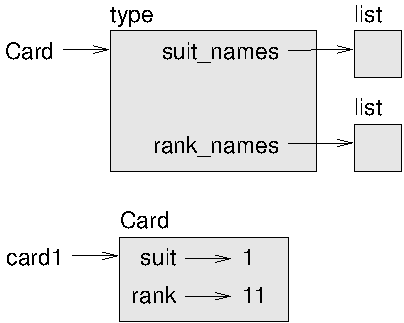
\includegraphics[scale=0.8]{figs/card1.pdf}}
\caption{对象图.}
\label{fig.card1}
\end{figure}

图~\ref{fig.card1}是{\tt Card}类对象和一个Card实例的对象图;
{\tt Card}是个类对象, 其类型是{\tt type}.  
{\tt card1}是{\tt Card}的一个实例, 
所以其类型是{\tt Card}.
为了节约空间, 我没有画出\verb"suit_names"和\verb"rank_names"的内容. 
\index{state diagram}
\index{diagram!state} \index{object diagram} \index{diagram!object}


\section{比较卡牌}
\label{comparecard}
\index{operator!relational}
\index{relational operator}

对于内置类型, 有比较运算符({\tt <}, {\tt >}, {\tt ==}, 等.)
可以比较值, 并判断一个值大于, 小于或者等于另一个. 
对于自定义类型, 我们可以提供一个表示``小于''的\verb"__lt__"方法, 
来覆盖内置运算符的操作. 
\index{programmer-defined type}
\index{type!programmer-defined}

\verb"__lt__" 接收两个参数, {\tt self}和{\tt other},
并在{\tt self}小于{\tt other}时返回{\tt True}.
\index{override}
\index{operator overloading}

然而卡牌的正确顺序并不明了. 
比如, 梅花3和方块2, 哪个更好?
一个等级高, 一个花色大. 
若要比较两个牌大小, 你首先需要确定等级和花色, 哪个更重要. 

答案取决于玩的何种游戏,
但简便起见, 我们定义花色更重要, 所以所有的黑桃大于任意方块, 以此类推. 
\index{cmp method@\_\_cmp\_\_ method}
\index{method!\_\_cmp\_\_}

定好规则, 我们便可以编写\verb"__lt__"了:

\begin{verbatim}
# inside class Card:

    def __lt__(self, other):
        # check the suits
        if self.suit < other.suit: return True
        if self.suit > other.suit: return False

        # suits are the same... check ranks
        return self.rank < other.rank
\end{verbatim}
%
使用元组来比较, 更加简洁:
\index{tuple!comparison}
\index{comparison!tuple}

\begin{verbatim}
# inside class Card:

    def __lt__(self, other):
        t1 = self.suit, self.rank
        t2 = other.suit, other.rank
        return t1 < t2
\end{verbatim}
%
做个练习, 为Time对象编写\verb"__lt__"方法. 
你可以用元组进行比较, 也可以考虑比较整数. 


\section{整幅牌}
\index{list!of objects}
\index{deck, playing cards}

现在我们有Card类了, 下一步要定义整副牌(Deck)了. 
既然整幅牌是由卡牌构成, 那自然每副牌都应该包含一个卡牌列表作为属性. 
\index{init method}
\index{method!init}

下面是{\tt Deck}的类定义. 
init方法新建了一个{\tt cards}属性, 
同时生成了标准的52张牌:
\index{composition}
\index{loop!nested}
\index{Deck class}
\index{class!Deck}

\begin{verbatim}
class Deck:

    def __init__(self):
        self.cards = []
        for suit in range(4):
            for rank in range(1, 14):
                card = Card(suit, rank)
                self.cards.append(card)
\end{verbatim}
%
生成一副牌最容易的方法便是嵌套循环了. 
外层循环枚举了0到3的花色. 
内层循环枚举了1至13的等级. 
每次迭代都会用当前花色和等级创建一张牌, 
并将其附加到{\tt self.cards}中. 
\index{append method}
\index{method!append}


\section{打印整幅牌}
\label{printdeck}
\index{str method@\_\_str\_\_ method}
\index{method!\_\_str\_\_}

下面是{\tt Deck}的\verb"__str__"方法:

\begin{verbatim}
# inside class Deck:

    def __str__(self):
        res = []
        for card in self.cards:
            res.append(str(card))
        return '\n'.join(res)
\end{verbatim}
%
这个方法展示了一个拼接超大字符串的高效方法: 建立一个字符串列表, 然后使用字符串方法{\tt join}进行拼接. 
内置函数{\tt str}会对每个card都应用\verb"__str__"方法, 以返回字符串格式.
\index{accumulator!string} \index{string!accumulator}
\index{join method} \index{method!join} \index{newline}

我们在换行符上调用了{\tt join}方法, 卡牌之间被分隔成了新行. 
下面是结果示例:

\begin{verbatim}
>>> deck = Deck()
>>> print(deck)
Ace of Clubs
2 of Clubs
3 of Clubs
...
10 of Spades
Jack of Spades
Queen of Spades
King of Spades
\end{verbatim}
%
虽然结果看起来是52行, 但它其实是一个包含换行符的长字符串. 


\section{添加, 移除, 洗牌和排序}

若要发牌, 首先需要一个能够从整副牌中移除并返回此对象的方法. 
列表方法{\tt pop}提供了一种便捷的方法:
\index{pop method}
\index{method!pop}

\begin{verbatim}
# inside class Deck:

    def pop_card(self):
        return self.cards.pop()
\end{verbatim}
%
由于{\tt pop}是从列表中移除{\em 最后一张}牌, 所以我们从底部发牌. 
\index{append method}
\index{method!append}

若要添加一张牌, 可以用列表方法{\tt append}:

\begin{verbatim}
# inside class Deck:

    def add_card(self, card):
        self.cards.append(card)
\end{verbatim}
%
像上面这样仅使用另一个方法, 而不做过多操作, 有时被称为{\bf veneer(装饰)}. 
这个比喻来自于木工行业, 在一块便宜木头表面贴一层优质的薄木板, 进行伪装, 
从而改善外观. 
\index{veneer}

这里, \verb"add_card" 是一个``薄''方法, 用卡牌术语的方式, 表达列表操作. 
而这会令实现的外观, 或者接口, 容易理解. 

再举个例子, 我们可以用{\tt random}模块中的{\tt shuffle}函数, 为Deck编写一个
{\tt shuffle}方法:
\index{random module}
\index{module!random}
\index{shuffle function}
\index{function!shuffle}

\begin{verbatim}
# inside class Deck:
            
    def shuffle(self):
        random.shuffle(self.cards)
\end{verbatim}
%
不要忘记引入{\tt random}模块.

做个练习, 用列表方法{\tt sort}为Deck编写一个{\tt sort}方法, 
为{\tt Deck}中的卡牌排序. 
{\tt sort}方法会使用我们定义的\verb"__lt__"方法来确定顺序. 
\index{sort method} \index{method!sort}



\section{继承}
\index{inheritance}
\index{object-oriented programming}

继承是一种基于已有类进行修改, 从而定义新类的能力. 
比如, 我们想要一个类来表示``手牌'', 即玩家手中持有的牌. 
一副手牌和整副牌相差无几: 都是由卡牌构成, 并且都需要支持添加和移除牌等操作. 

但二者也有差异: 有些手牌需要某些操作, 但整幅牌却不需要. 比如, 在
扑克牌中, 我们可能需要比较两幅手牌, 看哪个获胜. 
在桥牌中, 我们可能需要计算手牌的分数, 以便下注. 

类之间这种---相似却又不同---的关系, 非常适合使用继承. 
若要定义一个继承自现有类的新类, 只需要将现有类的名称放在括号中即可:
\index{parentheses!parent class in}
\index{parent class}
\index{class!parent}
\index{Hand class}
\index{class!Hand}

\begin{verbatim}
class Hand(Deck):
    """Represents a hand of playing cards."""
\end{verbatim}
%
这个定义表明{\tt Hand}继承自{\tt Deck};
也就是说, 我们可以像Deck一样对Hand应用\verb"pop_card"和\verb"add_card"方法.

当一个新类继承自现有类, 那么现有的类叫做{\bf 父类}, 
新的类叫做{\bf 子类}.
\index{parent class}
\index{child class}
\index{class!child}

在本例中, {\tt Hand}从{\tt Deck}继承了\verb"__init__"方法, 
但没有满足我们的需求: init方法本应用空列表初始化{\tt cards}, 
而不是用52张新牌. 
\index{override} \index{init method}
\index{method!init}

如果我们在{\tt Hand}类中提供了init方法, 那它会覆写{\tt Deck}类中的init方法:

\begin{verbatim}
# inside class Hand:

    def __init__(self, label=''):
        self.cards = []
        self.label = label
\end{verbatim}
%
当你创建一个Hand时, Python便会调用这个init方法, 而不是{\tt Deck}中的那个. 

\begin{verbatim}
>>> hand = Hand('new hand')
>>> hand.cards
[]
>>> hand.label
'new hand'
\end{verbatim}
%
其他的方法从{\tt Deck}继承而来, 所以我们可以用
\verb"pop_card"和\verb"add_card"方法来发牌:

\begin{verbatim}
>>> deck = Deck()
>>> card = deck.pop_card()
>>> hand.add_card(card)
>>> print(hand)
King of Spades
\end{verbatim}
%
很显然, 下一步就是要把这些代码封装进一个叫\verb"move_cards"的方法中:
\index{encapsulation}

\begin{verbatim}
# inside class Deck:

    def move_cards(self, hand, num):
        for i in range(num):
            hand.add_card(self.pop_card())
\end{verbatim}
%

\verb"move_cards"方法接受两个参数, 一个Hand对象, 一个发牌数量. 
同时它也会修改{\tt self}和{\tt hand}, 并返回{\tt None}.

在某些游戏中, 卡牌会从一副手牌, 移到另一副手牌, 或者
从手牌退还到牌堆中. 
你可以使用\verb"move_cards"来执行这些操作: {\tt self}可以是
一个Deck, 或者一副Hand, 尽管名字叫Hand, 但也可以是一个{\tt Deck}.

继承是种很有用的特性. 
某些没用继承的重复性代码, 使用继承可以变得更优雅. 
继承也方便了代码复用, 你可以通过修改父类行为, 
为子类都添加行为. 
在某些情况下, 继承的结构反映了问题的真正结构, 也就使得
设计更易于理解. 

另一方面, 继承会使程序变得难以阅读. 
当调用一个方法时, 有时很难搞明白它的定义在哪里. 
相关代码可能分散在数个模块. 
此外, 许多使用继承实现的事情, 不用继承也能做到, 甚至做得更好. 


\section{类图}
\label{class.diagram}

我们已经接触过表示程序状态的栈图, 以及展示对象的属性以及值的对象图. 
这些图好比程序运行时的快照, 因此也会随着程序运行而变化. 

它们通常很详细; 但对于某些目的来说, 偏于细致. 
类图是程序结构的一种更抽象的表达. 
它不展示单独对象, 而是表示类和类之间的关系. 

类之间有多种关系:

\begin{itemize}

\item 一个类中的对象可以包括其他类中对象的引用. 
例如, 每个Rectangle都包含了一个对Point的引用,
同时每个Deck包含了多个Card的引用. 
这种关系叫做{\bf 组合(HAS-A)}, 也就是, ``一个Rectangle有一个Point.''

\item 一个类可以继承自其他类. 
这种关系叫做{\bf 继承(IS-A)}, 就如, ``一个Hand是一种Deck.''

\item 一个类可能依赖于另一个类, 因为类中对象可能会将其他类中的对象作为参数
使用, 或者将其他类中的对象作为计算的一部分. 
这种关系, 叫做{\bf 依赖(dependency)}.

\end{itemize}
\index{IS-A relationship}
\index{HAS-A relationship}
\index{class diagram}
\index{diagram!class}

{\bf 类图}是这些关系的图形化表示. 比如, 图~\ref{fig.class1} 
展示了{\tt Card}, {\tt Deck}和{\tt Hand}之间的关系. 

\begin{figure}
\centerline
{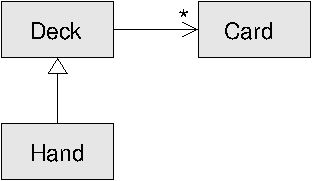
\includegraphics[scale=0.8]{figs/class1.pdf}}
\caption{类图.}
\label{fig.class1}
\end{figure}

空心三角箭头表示 IS-A 关系;
这里表示Hand继承自Deck. 

标准箭头表示HAS-A关系;
这里表示Deck包含Card对象的引用. 
\index{multiplicity (in class diagram)}

箭头附近的星号({\tt *})是一个{\bf 复数表达};
表示Deck包含多少个Card. 
复数表达可以是一个{\tt 52}一样的简单数字, 
可以是{\tt 5..7}一样的一个范围, 
或者一个星号, 表示Deck可以有任意个Card. 

此类图中没有依赖关系. 
依赖关系通常用虚线箭头表示. 
或者, 若有很多依赖关系存在, 它们有时候会被省略. 

一个更详细的类图, 可能会显示Deck实际上包含了一个Card{\em 列表}, 
但是一般类图中不包含列表和字典这些内置类型. 

\section{调试}
\index{debugging}

继承可能会令调试变得困难, 因为当你调用对象的方法时, 
可能很难确定是调用的哪个方法. 
\index{inheritance}

假设你正在写一个处理Hand对象的函数. 
你希望适用于各种牌型, 比如PokerHands, BridgeHands, 等等. 
如果你调用像{\tt Shuffle}这样的方法, 
你可能用的是{\tt Deck}中定义的方法, 
但如果子类重写了这个方法, 
你调用的便是子类中的方法了. 
这个特性说来是好事, 但有时令人困惑. 

如果你不确定程序执行流程的时候, 最简单的方法便是在相关方法
开始处添加打印语句, 输出信息. 
如果{\tt Deck.shuffle}打印了一条信息, 如{\tt Running Deck.shuffle}, 
那便可以据此来追踪执行流程. 
\index{flow of execution}

另一个思路, 你可以用下面的函数, 接收对象和方法名称(字符串表示), 
然后返回提供该方法定义的类:

\begin{verbatim}
def find_defining_class(obj, meth_name):
    for ty in type(obj).mro():
        if meth_name in ty.__dict__:
            return ty
\end{verbatim}
%
下面是个示例:

\begin{verbatim}
>>> hand = Hand()
>>> find_defining_class(hand, 'shuffle')
<class '__main__.Deck'>
\end{verbatim}
%
这样便可以知道Hand中的{\tt shuffle}方法来自于{\tt Deck}.
\index{mro method}
\index{method!mro}
\index{method resolution order}

\verb"find_defining_class"函数使用{\tt mro}方法, 获取类对象的列表, 
进而根据方法进行搜索. 
``MRO''是``method resolution order''的简称, 
是指Python``解析''方法名时所搜索的序列.

下面是个设计建议: 当你覆盖一个方法时, 
新方法的接口, 要和旧的保持一致. 
它应该接收同样的参数, 返回相同的类型, 
同时遵守相同的先决条件和后置条件. 
如果你遵循上述规则, 你会发现为父类实例, 如Deck, 所设计的函数, 
也同样适用于子类实例, 比如Hand和PokerHand. 

\index{override}
\index{interface}
\index{precondition}
\index{postcondition}

如果你违反了这个``里氏替换原理''原则, 
那代码将很不幸地像纸牌屋一样崩塌. 
\index{Liskov substitution principle}


\section{数据封装}

前面章节讲述了一种``面向对象设计''的开发模式. 
我们识别了对象--比如{\tt Point}, {\tt Rectangle}和{\tt Time}---同时
定义类来表示这些对象. 
在每个例子中, 对象和现实世界(或者至少是数学世界)实体之间一般都有明显的对应关系. 
\index{development plan!data encapsulation}

但有时候很难界定所需的对象以及如何与之交互. 
这种情况下, 你需要一个不同的开发模式. 
之前我们通过封装和泛化来设计函数接口, 同样我们也可以通过{\bf 数据封装}
来设计类接口. 
\index{data encapsulation}

第~\ref{markov}节的马尔可夫分析, 便是一个很好的例子. 
如果你从\url{http://thinkpython2.com/code/markov.py}下载我的代码, 
你会看到使用了两个全局变量---\verb"suffix_map" 和
\verb"prefix"---会被多个函数读写. 

\begin{verbatim}
suffix_map = {}        
prefix = ()            
\end{verbatim}

因为这些变量是全局的, 我们一次只能运行一个分析. 
如果我们读取两个文本, 他们的前置和后置词汇都会被添加到同一个数据结构
中(会生成一些有趣的文本). 

若要运行多个分析, 同时保持互不影响, 我们可以把每个分析的状态封装到对象中. 
代码如下:

\begin{verbatim}
class Markov:

    def __init__(self):
        self.suffix_map = {}
        self.prefix = ()    
\end{verbatim}

接下来, 我们把函数转换为方法. 
下面是\verb"process_word"方法的示例:

\begin{verbatim}
    def process_word(self, word, order=2):
        if len(self.prefix) < order:
            self.prefix += (word,)
            return

        try:
            self.suffix_map[self.prefix].append(word)
        except KeyError:
            # if there is no entry for this prefix, make one
            self.suffix_map[self.prefix] = [word]

        self.prefix = shift(self.prefix, word)        
\end{verbatim}
像这样修改程序---改变设计而不改变其行为---便是另一种重构
(参见第~\ref{refactoring}节).
\index{refactoring}

这个例子展示了一种新的设计对象和方法的开发模式:

\begin{enumerate}

\item 先编写读写全局变量的函数(如有必要).

\item 一旦程序可以运行, 便可寻找全局变量和使用它们的函数之间的关联.

\item 将相关变量封装为对象的属性.

\item 将相关函数转换为新类的方法.

\end{enumerate}

做个练习, 从\url{http://thinkpython2.com/code/markov.py}下载笔者的马尔可夫代码, 
遵循上述步骤, 将全局变量封装为新类{\tt Markov}的属性. 
解决方案代码见\url{http://thinkpython2.com/code/markov2.py}.



\section{术语表}

\begin{description}

\item[编码(encode):] 通过建立一个映射, 用另一组值来表示一组值的过程.
\index{encode}

\item[类属性(class attribute):] 类对象中的属性. 类属性定义在类定义的内部, 
但在方法外部. 
\index{class attribute}
\index{attribute!class}

\item[实例属性(instance attribute):] 与类实例关联的属性.
\index{instance attribute}
\index{attribute!instance}

\item[伪装方法(veneer):] 一个方法或者函数, 无需太多计算便可以为其他方法提供不同的接口. 
\index{veneer}

\item[继承(inheritance):] 定义新类的能力, 这个新类是先前定义的类的修改版本. 
\index{inheritance}

\item[父类(parent class):] 子类所继承的类.
\index{parent class}

\item[子类(child class):] 通过继承现有类而创建的新类; 也叫做``派生类''. 
\index{child class}
\index{class!child}

\item[IS-A关系(IS-A relationship):] 子类和其父类之间的关系.
\index{IS-A relationship}

\item[HAS-A关系(HAS-A relationship):] 指两个类之间, 一个类实例包含了
另一个类实例的引用.
\index{HAS-A relationship}

\item[依赖(dependency):] 两个类之间的关系, 
一个类的实例使用了另一个类的实例, 但没有将其作为属性存储. 
\index{HAS-A relationship}

\item[类图(class diagram):] 表示程序中各个类及其之间关系的图解. 
\index{class diagram}
\index{diagram!class}

\item[多倍数(multiplicity):] 类图中一种符号, 
用于表示HAS-A关系中一个类中对另一个类的实例引用的数量. 
\index{multiplicity (in class diagram)}

\item[数据封装(data encapsulation):] 一种开发模式, 
起始用全局变量出原型, 最后将全局变量均变为实例属性, 从而产生最终版本. 
\index{data encapsulation}
\index{development plan!data encapsulation}

\end{description}


\section{习题集}

\begin{exercise}
针对下面的程序, 绘制UML类图, 展示其中的类和类之间的关系. 

\begin{verbatim}
class PingPongParent:
    pass

class Ping(PingPongParent):
    def __init__(self, pong):
        self.pong = pong


class Pong(PingPongParent):
    def __init__(self, pings=None):
        if pings is None:
            self.pings = []
        else:
            self.pings = pings

    def add_ping(self, ping):
        self.pings.append(ping)

pong = Pong()
ping = Ping(pong)
pong.add_ping(ping)
\end{verbatim}


\end{exercise}



\begin{exercise}
编写Deck的\verb"deal_hands"方法, 使其接收两个参数, 分别为手牌数量以及每副手牌所含的卡牌数量. 
此方法会创建相应数量的手牌对象, 给每幅手牌分配相应数量的卡牌, 然后返回一个手牌实例的列表. 
\end{exercise}


\begin{exercise}
\label{poker}
下面是德州扑克中的可能牌型, 按照价值升序以及出现概率降序排列:
\index{poker}

\begin{description}

\item[一对:] 两张同样大小的牌
\vspace{-0.05in}

\item[两对:] 两对同样大小的牌
\vspace{-0.05in}

\item[三条:] 三张同样大小的牌
\vspace{-0.05in}

\item[顺子:] 顺序相连的五张牌 (A牌可以表示最高也可以表示最低的牌
, 所有{\tt A-2-3-4-5}是顺子, 同时{\tt
10-J-Q-K-A}也是顺子, 但是 {\tt Q-K-A-2-3} 不是顺子.)
\vspace{-0.05in}

\item[同花:] 五张同样花色的牌
\vspace{-0.05in}

\item[葫芦:] 三张同样大小的牌, 外加两张同样大小的牌
\vspace{-0.05in}

\item[四条:] 四张同样大小的牌
\vspace{-0.05in}

\item[同花顺:] 五张同花色的顺子
\vspace{-0.05in}

\end{description}
%
本练习主要用来估算抽到各种牌型的概率.

\begin{enumerate}

\item 从\url{http://thinkpython2.com/code}下载以下文件:

\begin{description}

\item[{\tt Card.py}]: 本章涉及的{\tt Card},
{\tt Deck}和{\tt Hand}类的完整版本. 

\item[{\tt PokerHand.py}]: 一个表示手牌类的不完整版本, 同时包含一些测试代码.

\end{description}
%
\item 如果运行 {\tt PokerHand.py}, 它将发放七张牌, 
并检查其中是否包含同花. 先仔细阅读代码, 再继续下面的操作. 

\item 向{\tt PokerHand.py}中添加一些方法, 可以叫\verb"has_pair",
\verb"has_twopair", 等等. 使其判断手牌是否满足特定要求, 而返回True或False. 
你的代码适用于任意数量的``手牌''(虽然5和7是常见的牌数). 

\item 编写名为{\tt classify}的方法, 使其标识出手牌中最高价值的牌型, 
并设置对应的{\tt label}属性. 比如, 一副七张牌的手牌, 
可能包含同花和一对;
那应将其标记为``同花''.

\item 当你确信分类方法正确无误, 下一步便是估算各种牌型出现的概率. 
在{\tt PokerHand.py}中编写函数, 完成洗牌, 分牌, 手牌分类, 
统计各种分类出现的次数. 

\item 打印一个表格, 显示各种分类及其出现概率. 
用大量手牌, 不断运行程序, 直到输出结果收敛于合理区间. 
把你得到的结果和\url{http://en.wikipedia.org/wiki/Hand_rankings}上的结果进行比较. 

\end{enumerate}

参考答案: \url{http://thinkpython2.com/code/PokerHandSoln.py}.
\end{exercise}


\chapter{利器}

本书中我一个主要目标便是尽量少提Python. 
当有两种方法可以实现同一个功能, 我会选择一种并避免提及另一种. 
有时我会将第二种方法放进习题中. 

现在我们回过头来介绍一些之前被忽略的好东西. 
Python 提供了一些虽非必要, 但好用的功能---你不用这些功能仍然可以写出好代码---但是
使用了这些技巧, 有时可以编写更简洁, 易读, 高效的代码, 甚至有时能同时兼顾这三个目标. 

% TODO: add the with statement

\section{条件表达式}

我们在第~\ref{conditional.execution}节见过条件语句. 
条件语句通常用来二选一; 比如:
\index{conditional expression}
\index{expression!conditional}

\begin{verbatim}
if x > 0:
    y = math.log(x)
else:
    y = float('nan')
\end{verbatim}

这个语句检验{\tt x} 是否是正数. 
如果是, 则计算{\tt math.log}. 
如果不是, {\tt math.log}则会抛出一个ValueError.
为了避免程序异常退出, 我们使用一个``NaN'', 这个符号是一个特殊的浮点数, 
表示``不是一个数字''. 
\index{NaN}
\index{floating-point}

我们可用一个{\bf 条件表达式}来更简洁编写此语句:

\begin{verbatim}
y = math.log(x) if x > 0 else float('nan')
\end{verbatim}

你可以像读英语一样读这行代码: ``{\tt y} gets log-{\tt x}
if {\tt x} is greater than 0; otherwise it gets NaN''.

递归函数有时候可以用条件表达式重写. 
比如, 下面是一个{\tt 阶乘}函数的递归版本:
\index{factorial}
\index{function!factorial}

\begin{verbatim}
def factorial(n):
    if n == 0:
        return 1
    else:
        return n * factorial(n-1)
\end{verbatim}

我们可以重写为:

\begin{verbatim}
def factorial(n):
    return 1 if n == 0 else n * factorial(n-1)
\end{verbatim}

条件表达式的另一个用途是处理可选参数. 
比如, 下面是{\tt GoodKangaroo}(参见习题~\ref{kangaroo})中的
init方法:
\index{optional argument}
\index{argument!optional}

\begin{verbatim}
    def __init__(self, name, contents=None):
        self.name = name
        if contents == None:
            contents = []
        self.pouch_contents = contents
\end{verbatim}

我们可以这样改写:

\begin{verbatim}
    def __init__(self, name, contents=None):
        self.name = name
        self.pouch_contents = [] if contents == None else contents 
\end{verbatim}

通常, 如果条件语句的两个分支都是简单表达式, 要么是被返回, 要么是被赋给同一变量, 
那么你便可以用条件表达式替换条件语句. 
\index{conditional statement}
\index{statement!conditional}



\section{列表推导式}

在第~\ref{filter}节, 我们学习了map和filter模式. 
比如, 下面函数接收一个字符串列表, 将字符串方法{\tt capitalize}映射到每个元素上, 
并返回一个新的字符串列表:

\begin{verbatim}
def capitalize_all(t):
    res = []
    for s in t:
        res.append(s.capitalize())
    return res
\end{verbatim}

我们可以用{\bf 列表推导式}来精简此函数:
\index{list comprehension}

\begin{verbatim}
def capitalize_all(t):
    return [s.capitalize() for s in t]
\end{verbatim}

方括号操作符表示我们在构造一个新列表. 
方括号中的表达式, 指定了列表中的元素, 同时{\tt for}语句声明了我们要遍历的序列. 
\index{list}
\index{for loop}

列表推导式的语法略显奇怪, 主要因为这个循环变量, 如例子中的{\tt s}, 在定义之前, 
便出现在了表达式中. 
\index{loop variable}

列表推导式也可以用来过滤. 
比如, 下面函数仅选择{\tt t}中大写字母的元素, 并返回新列表:
\index{filter pattern}
\index{pattern!filter}

\begin{verbatim}
def only_upper(t):
    res = []
    for s in t:
        if s.isupper():
            res.append(s)
    return res
\end{verbatim}

我们可以用列表推导式来重写:

\begin{verbatim}
def only_upper(t):
    return [s for s in t if s.isupper()]
\end{verbatim}

列表推导式更加简洁, 也更易读, 至少对于简单表达式是这样的. 
而且, 它们相比同样的for循环, 要更快, 甚至有时快很多. 
所以如果你因为我没有更早提及而生气, 我理解. 

但是, 我要申辩一下, 列表推导式通常更难调试, 
因为你不能在循环内部放置一个打印语句. 
我建议你只在计算足够简单的情况, 也就是你上手便能正确完成的时候使用. 
对于新手来说, 尽量别用. 
\index{debugging}



\section{生成器表达式}

{\bf 生成器表达式}和列表推导式相似, 但它使用圆括号而不是方括号:
\index{generator expression}
\index{expression!generator}

\begin{verbatim}
>>> g = (x**2 for x in range(5))
>>> g
<generator object <genexpr> at 0x7f4c45a786c0>
\end{verbatim}
%
结果是一个生成器对象, 同时其知晓如何遍历一个值序列. 
但是与列表推导式不同, 它不会立即计算所有值; 而是在被调用时才计算. 
内置函数{\tt next}会从生成器获取下一个值:
\index{generator object}
\index{object!generator}

\begin{verbatim}
>>> next(g)
0
>>> next(g)
1
\end{verbatim}
%
当抵达了序列末尾, {\tt next}会抛出一个StopIteration异常. 
你也可以使用{\tt for}循环来遍历这些值:
\index{StopIteration}
\index{exception!StopIteration}

\begin{verbatim}
>>> for val in g:
...     print(val)
4
9
16
\end{verbatim}
%
生成器对象会跟踪序列中的位置, 
所以{\tt for}循环会在{\tt next}停止的地方开始. 
一旦生成器被耗尽, 依然会抛出{\tt StopIteration}:

\begin{verbatim}
>>> next(g)
StopIteration
\end{verbatim}

生成器表达式通常和{\tt sum},
{\tt max}, 以及{\tt min}等函数一起使用:
\index{sum}
\index{function!sum}

\begin{verbatim}
>>> sum(x**2 for x in range(5))
30
\end{verbatim}


\section{{\tt any} 和 {\tt all}}

Python提供了一个内置函数, {\tt any}, 其接收一个布尔值序列, 
如果任意一个值为{\tt True}, 则返回{\tt True}. 通常适用于列表:
\index{any}
\index{built-in function!any}

\begin{verbatim}
>>> any([False, False, True])
True
\end{verbatim}
%
但也多用于生成器表达式:
\index{generator expression}
\index{expression!generator}

\begin{verbatim}
>>> any(letter == 't' for letter in 'monty')
True
\end{verbatim}
%
这个例子不太明显, 因为和{\tt in}运算符的效果一样. 
但我们可以用{\tt any}来重写第~\ref{search}节中, 曾经写的一些搜索函数. 
例如, 我们可以如下改写{\tt avoids}:
\index{search pattern}
\index{pattern!search}

\begin{verbatim}
def avoids(word, forbidden):
    return not any(letter in forbidden for letter in word)
\end{verbatim}
%
这个函数可以像读英语那样理解, ``{\tt word} avoids
{\tt forbidden} if there are not any forbidden letters in {\tt word}.
(如果{\tt 单词}中不包含任何禁用字母, 那么{\tt 单词}便避免{\tt 被禁用})''

将{\tt any}和生成器表达式一起使用, 效率更高, 因为只要遇到{\tt True}值, 它便会立刻停止, 
所以不会计算整个序列. 

Python还提供了另一个内置函数, {\tt all}, 如果序列中每个元素都是{\tt True}, 
那么它便会返回{\tt True}.
作为练习, 用{\tt all}重写第~\ref{search}节的\verb"uses_all"函数.
\index{all}
\index{built-in function!any}


\section{集合(set)}
\label{sets}

在第~\ref{dictsub}节, 我用字典来寻找出现在文档中, 但是不在单词列表中的单词. 
该函数接收两个参数, 包含文档中单词的参数{\tt d1}(作为键),  和包含单词列表的参数{\tt d2}. 
最后返回一个字典, 其键存在于{\tt d1}中, 但不包含在{\tt d2}中. 

\begin{verbatim}
def subtract(d1, d2):
    res = dict()
    for key in d1:
        if key not in d2:
            res[key] = None
    return res
\end{verbatim}
%
在这些字典中, 值都是{\tt None}, 因为从没有使用它们. 
结果就是我们浪费了一些存储空间. 
\index{dictionary subtraction}

Python提供了另一种内置类型, 叫做{\tt set}, 
其效果很像字典中没有值的键的集合. 
向集合中添加元素是很快的; 检查成员也很快. 
同时集合也提供了执行常见操作的方法和运算符. 
\index{set}
\index{object!set}

比如, 集合的差集操作有{\tt difference}方法, 或者{\tt -}操作符. 
所以我们可以将{\tt subtract}像下面一样重写:
\index{set subtraction}

\begin{verbatim}
def subtract(d1, d2):
    return set(d1) - set(d2)
\end{verbatim}
%
结果是一个集合, 而不是字典, 
但对于像迭代这样的操作, 其行为是相同的. 

本书中的一些练习题可以用集合进行精简和优化. 
比如, 下面是习题~\ref{duplicate}中, 使用字典解决\verb"has_duplicates"的一个方案:

\begin{verbatim}
def has_duplicates(t):
    d = {}
    for x in t:
        if x in d:
            return True
        d[x] = True
    return False
\end{verbatim}

当一个元素首次出现, 则被加入字典. 
如果同一元素再次出现, 函数返回{\tt True}. 

使用集合, 我们可以如下一般, 实现相同的函数:

\begin{verbatim}
def has_duplicates(t):
    return len(set(t)) < len(t)
\end{verbatim}
%
一个元素在集合中只能出现一次, 所以如果{\tt t}中有元素出现多次, 那么集合长度必然小于
{\tt t}的长度. 
如果没有重复的, 集合大小和{\tt t}的大小相同. 
\index{duplicate}

我们也可以使用集合完成第~\ref{wordplay}节的某些习题. 
比如, 下面是一个使用循环的\verb"uses_only"实现版本:

\begin{verbatim}
def uses_only(word, available):
    for letter in word: 
        if letter not in available:
            return False
    return True
\end{verbatim}
%
\verb"uses_only"会检查{\tt word}中所有字母是否都在{\tt available}中.
我们可以像这样重写:

\begin{verbatim}
def uses_only(word, available):
    return set(word) <= set(available)
\end{verbatim}
%

运算符\verb"<=" 会检验一个集合是否是另一个的子集, 包括两者相等的情况, 
也就是如果{\tt word}中的字母都出现在{\tt available}, 则返回真. 
\index{subset}

做个练习, 使用集合重写\verb"avoids". 


\section{计数器(Counter)}

{\bf Counter(计数器)}类似于集合, 不同之处在于如果一个元素出现多次, 计数器会跟踪其出现次数. 
如果你熟悉数学概念中的{\bf 多重集合}, 便会发现计数器是表示多重集合的一种自然方式. 
\index{Counter}
\index{object!Counter}
\index{multiset}

计数器定义在{\tt collections}标准模块中, 
所以你需要先导入. 
你可以用字符串, 列表或者支持迭代的任意类型来初始化计数器. 
\index{collections}
\index{module!collections}

\begin{verbatim}
>>> from collections import Counter
>>> count = Counter('parrot')
>>> count
Counter({'r': 2, 't': 1, 'o': 1, 'p': 1, 'a': 1})
\end{verbatim}

计数器和字典在表现上相似之处颇多;
它们都是将每个键映射到其出现次数. 
和字典一样, 键必需是可哈希的. 

与字典不同, 如果你访问一个不存在的元素, 计数器不会抛出异常, 而是返回0:

\begin{verbatim}
>>> count['d']
0
\end{verbatim}

我们可以用计数器来重写习题~\ref{anagram}中的\verb"is_anagram"函数:

\begin{verbatim}
def is_anagram(word1, word2):
    return Counter(word1) == Counter(word2)
\end{verbatim}

如果两个单词是换位词, 那么它们的相同字母具有相同的数量, 因此它们的计数器是等价的. 

计数器提供了一些类似集合操作的方法和运算符, 
包括方法, 减法, 并集和交集. 
此外, 还提供了一个常用的方法, \verb"most_common", 这个方法
会返回一个按照最常见到最不常见排序的值-频率对列表:

\begin{verbatim}
>>> count = Counter('parrot')
>>> for val, freq in count.most_common(3):
...     print(val, freq)
r 2
p 1
a 1
\end{verbatim}

\section{默认字典(defaultdict)}

{\tt collections}模块同时提供了{\tt defaultdict(默认字典)}, 
其与字典类似, 不同之处在于, 如果你访问一个不存在的键, 它可以即刻生成一个新值. 
\index{defaultdict}
\index{object!defaultdict}
\index{collections}
\index{module!collections}

当你创建默认字典时, 你需要提供一个函数, 以用于创建新值. 
用来创建对象的函数, 有时也称为{\bf 工厂}.
创建列表, 集合, 以及其他类型的内置函数, 都可以称为工厂:
\index{factory function}

\begin{verbatim}
>>> from collections import defaultdict
>>> d = defaultdict(list)
\end{verbatim}

注意这个函数的参数{\tt list}, 是个类对象, 
而不是一个新列表{\tt list()}. 
而且只有在访问不存在的键时, 才会调用提供的函数.

\begin{verbatim}
>>> t = d['new key']
>>> t
[]
\end{verbatim}

新的列表, 也就是{\tt t}, 便被加入了字典中. 
所以, 如果我们修改{\tt t}, {\tt d}也会相应变化:

\begin{verbatim}
>>> t.append('new value')
>>> d
defaultdict(<class 'list'>, {'new key': ['new value']})
\end{verbatim}

如果你要创建一个值为列表的字典, 可以使用{\tt defaultdict}来简化代码. 
在习题~\ref{anagrams}的答案(可以从\url{http://thinkpython2.com/code/anagram_sets.py}获取)中, 
我创建了一个字典, 该字典将一个有序字母的字符串映射到了一个由这些字母构成的单词的列表. 
比如, {\tt 'opst'}映射了列表{\tt ['opts', 'post', 'pots', 'spot', 'stop', 'tops']}.

下面是原始代码:

\begin{verbatim}
def all_anagrams(filename):
    d = {}
    for line in open(filename):
        word = line.strip().lower()
        t = signature(word)
        if t not in d:
            d[t] = [word]
        else:
            d[t].append(word)
    return d
\end{verbatim}

这里可以用{\tt setdefault}来简化代码, 你可能已经在练习~\ref{setdefault}中使用过:
\index{setdefault}

\begin{verbatim}
def all_anagrams(filename):
    d = {}
    for line in open(filename):
        word = line.strip().lower()
        t = signature(word)
        d.setdefault(t, []).append(word)
    return d
\end{verbatim}

但此方案也略有不足, 其不论是否必要, 每次都会创建新列表. 
对于列表来说, 尚无关紧要, 但如果工厂函数很复杂, 
那影响就很大了. 
\index{factory function}

我们可以用{\tt defaultdict}来避免这个问题, 并简化代码:

\begin{verbatim}
def all_anagrams(filename):
    d = defaultdict(list)
    for line in open(filename):
        word = line.strip().lower()
        t = signature(word)
        d[t].append(word)
    return d
\end{verbatim}

对于习题~\ref{poker}, 你可以从
\url{http://thinkpython2.com/code/PokerHandSoln.py}下载我的方案, 
在函数\verb"has_straightflush"中使用了{\tt setdefault}. 
这个方案也有缺陷, 不论是否需要, 每次循环都会创建{\tt Hand}对象. 
作为一项练习, 试试用{\tt defaultdict}来重写它. 


\section{命名元组}
\label{Named tuples}

许多简单对象基本都是相关值的集合. 
比如, 第~\ref{clobjects}节的Point对象包含两个数值, {\tt x}和{\tt y}.
当你像下面一样定义类时, 通常会从{\tt init}方法和{\tt str}方法开始:

\begin{verbatim}
class Point:

    def __init__(self, x=0, y=0):
        self.x = x
        self.y = y

    def __str__(self):
        return '(%g, %g)' % (self.x, self.y)
\end{verbatim}

传递如此少的信息, 竟使用了如此多的代码, 杀鸡用了牛刀. 
Python提供了一个更加简洁的方法实现同样的事情:

\begin{verbatim}
from collections import namedtuple
Point = namedtuple('Point', ['x', 'y'])
\end{verbatim}

第一个参数是你要创建的类的名称. 
第二个参数是Point对象应具有的属性列表, 都用字符串表示. 
最后, {\tt namedtuple}的返回值是一个类对象:
\index{namedtuple}
\index{object!namedtuple}
\index{collections}
\index{module!collections}

\begin{verbatim}
>>> Point
<class '__main__.Point'>
\end{verbatim}

{\tt Point}自动构建了\verb"__init__"和
\verb"__str__"这样的方法, 所以你无需自己编写它们. 
\index{class object}
\index{object!class}

若要创建Point对象, 只需要将Point类作为函数使用:

\begin{verbatim}
>>> p = Point(1, 2)
>>> p
Point(x=1, y=2)
\end{verbatim}

{\tt init}方法将参数赋值给你命名的属性. 
{\tt str}方法会输出字符串格式的Point类及其属性. 

你可以通过名字访问命名元组的元素:

\begin{verbatim}
>>> p.x, p.y
(1, 2)
\end{verbatim}

也可以将命名元组作为一个元组来操作:

\begin{verbatim}
>>> p[0], p[1]
(1, 2)

>>> x, y = p
>>> x, y
(1, 2)
\end{verbatim}

命名元组提供了一种定义简单类的快捷方式. 
不足之处在于, 简单的类不会一直简单下去. 
后续你可能想给一个命名元组添加方法. 
遇到这种情况, 你可以定义一个继承自命名元组的新类:
\index{inheritance}

\begin{verbatim}
class Pointier(Point):
    # add more methods here
\end{verbatim}

或者你可以回到传统的类定义方案. 


\section{收集关键字参数}

在第~\ref{gather}节, 我们已经学到如何编写将参数收集到元组的函数:
\index{gather}

\begin{verbatim}
def printall(*args):
    print(args)
\end{verbatim}
%
你可以用任意数量的位置参数(即无关键字的参数)来调用此函数:
\index{positional argument}
\index{argument!positional}

\begin{verbatim}
>>> printall(1, 2.0, '3')
(1, 2.0, '3')
\end{verbatim}
%
然而{\tt *}运算符不会收集关键字参数:
\index{keyword argument}
\index{argument!keyword}

\begin{verbatim}
>>> printall(1, 2.0, third='3')
TypeError: printall() got an unexpected keyword argument 'third'
\end{verbatim}
%
若要收集关键字参数, 可以使用{\tt **}运算符:

\begin{verbatim}
def printall(*args, **kwargs):
    print(args, kwargs)
\end{verbatim}
%
你可以将关键字收集参数命名为任意名称, 但一般常用{\tt kwargs}命名. 
其结果便是一个从关键字映射到值的字典:

\begin{verbatim}
>>> printall(1, 2.0, third='3')
(1, 2.0) {'third': '3'}
\end{verbatim}
%
同样, 如果你有一个映射关键字和值的字典, 也可以在调用函数时, 
使用发散运算符{\tt **}:
\index{scatter}

\begin{verbatim}
>>> d = dict(x=1, y=2)
>>> Point(**d)
Point(x=1, y=2)
\end{verbatim}
%
如果没用发散运算符, 函数会将{\tt d}当作一个位置参数, 
所以便会将{\tt d}赋值给{\tt x}, 同时报错, 因为没有对{\tt y}进行赋值:

\begin{verbatim}
>>> d = dict(x=1, y=2)
>>> Point(d)
Traceback (most recent call last):
  File "<stdin>", line 1, in <module>
TypeError: __new__() missing 1 required positional argument: 'y'
\end{verbatim}
%
当你需要处理具有大量参数的函数时, 
创建并传递声明了常用关键字的字典, 会比较高效. 


\section{术语表}

\begin{description}

\item[条件表达式(conditional expression):] 基于条件, 进行二选一抉择的表达式.
\index{conditional expression}
\index{expression!conditional}

\item[列表推导式(list comprehension):] 一种方括号内包含{\tt for}循环, 产生新列表的表达式.
\index{list comprehension}

\item[生成器表达式(generator expression):] 一种圆括号内包含{\tt for}循环, 
从而产生生成器对象的表达式.  
\index{generator expression}
\index{expression!generator}

\item[多重集合(multiset):] 一种表示集合中元素与其出现次数的数学概念.

\item[工厂(factory):] 用来创建对象的函数, 通常作为参数传递. 
\index{factory}

\end{description}




\section{习题集}

\begin{exercise}

下面是个递归计算二项式系数的函数.

\begin{verbatim}
def binomial_coeff(n, k):
    """Compute the binomial coefficient "n choose k".

    n: number of trials
    k: number of successes

    returns: int
    """
    if k == 0:
        return 1
    if n == 0:
        return 0

    res = binomial_coeff(n-1, k) + binomial_coeff(n-1, k-1)
    return res
\end{verbatim}

使用嵌套条件表达式优化函数体.

提示: 因为这个函数最终会不断重复计算相同的值, 所以不够高效. 
你可以使用缓存模式(参见第~\ref{memoize}节)来提升其效率. 
但是你会发现, 一旦使用了条件表达式, 缓存实现便变得困难. 
\end{exercise}



\appendix

\chapter{调试}
\index{debugging}

在调试阶段, 你要对不同类型错误进行区分, 从而快速定位:

\begin{itemize}

\item 语法错误多出现在解释器翻译源码为字节码的时候. 
通常表示程序结构有缺陷. 
比如: {\tt def}语句后面遗漏了冒号, 会出现{\tt SyntaxError: invalid syntax}这样的信息.
\index{syntax error}
\index{error!syntax}

\item 运行时异常多在程序运行过程中, 因解释器出错而产生. 
多数运行时异常信息包括异常发生的位置以及所执行的函数. 
比如: 一个无尽的递归, 终会导致运行时异常, 出现``maximum recursion depth exceeded''报错信息.
\index{runtime error}
\index{error!runtime}
\index{exception}

\item 语义异常多指程序运行不报错, 但结果不正确.
比如: 表达式没有按你期望的顺序执行, 从而产生了错误的结果.
\index{semantic error}
\index{error!semantic}

\end{itemize}

调试的第一步, 是明确你面对的是何种异常. 
虽然下面章节都是按照异常类型所组织, 但有些技巧也适用于其他情况. 


\section{语法异常}
\index{error message}

如果你能弄清程序的语法异常是什么, 便很容易修复. 
不幸的是, 错误提示往往无用. 常见的多是{\tt SyntaxError: invalid syntax}和
{\tt SyntaxError: invalid token}, 都是大而无用的笼统概括. 

但另一方面, 错误信息确实告诉了你程序异常发生的位置. 
实际上, 是告知你Python所认为的异常所在, 但不一定就是错误确实发生的地方. 
有时候, 错误信息先于错误的位置信息出现, 通常在前一行. 
\index{incremental development}
\index{development plan!incremental}
如果你是逐步构建程序, 你便很容易定位错误所在. 其通常出现在你最后添加的代码中. 

如果你正从书中复制代码, 从一开始, 便需要仔细比较你的代码和书中的代码. 
检查每个字符. 同时, 要谨记, 书中可能有错误, 所以你若看到了某些语法异常的代码, 
那可能真是语法异常. 

下面是一些避免产生常见语法错误的方法:
\index{syntax}

\begin{enumerate}

\item 确保你没有用Python关键字作为变量名. 
\index{keyword}

\item 检查每个复合语句的头部末尾是否都写了冒号, 包括{\tt for}, {\tt while},
{\tt if}, 和{\tt def}语句. 
\index{header}
\index{colon}

\item 确保代码中所有字符串都有成对的引号. 确保所有的引号都是``直引号'', 而不是``弯引号''. 
\index{quotation mark}

\item 如果你有三个引号(单引号或者双银行)包起来的多行字符串, 确保正确终止了字符串. 
未终止的字符串可能会在程序末尾引发{\tt invalid token}异常, 
或者可能会将程序余下部分当作字符串, 直至碰到下个字符串的标识. 
而在第二种情形下, 可能不会产生错误信息!
\index{multiline string}
\index{string!multiline}

\item 未封闭的开放运算符---\verb+(+, \verb+{+, 或
\verb+[+---会使Python将下一行作为当前语句的一部分处理. 
通常, 下一行立刻会报错. 

\item 检查条件表达式中是否使用了经典的{\tt =}, 而不是{\tt ==}.
\index{conditional}

\item 检查缩进是否都对齐. Python可以使用空格和制表符, 但如果你
混用, 很可能会引发问题. 
避免这种问题的最好方式, 是使用了解Python并能生成一致性缩进的文本编辑器. 
\index{indentation}
\index{whitespace}

\item 如果代码中有非-ASCII字符(无论字符串还是注释), 都会引发一场, 
即使Python 3通常可以处理非-ASCII字符. 
所以你从网页或者其他地方复制文本的时候要当心. 

\end{enumerate}

如果还不起作用, 那进行下一步操作吧...


\subsection{不断修正, 却毫无作用.}

如果解释器说有个错误, 但你总是找不到, 
那可能是因为你和解释器看到的不是相同的代码. 
检查编码环境, 确保你编辑的便是Python运行的程序. 

如果你不确定, 则可以在程序开始的地方, 放个明显且可控的异常. 
然后再次运行, 如果编译器没有报错, 那你便不是在运行最新的代码. 


下面是几个可能的元凶:

\begin{itemize}

\item 修改了文件, 但再次运行前忘记保存更改. 有些编程环境可以自动保存, 但有些不会. 

\item 修改了文件名, 但仍用旧的文件名运行. 

\item 开发环境设置不正确. 

\item 如果你编写了个模块, 并使用了{\tt import}语句, 一定要确保
没有和标准Python模块同名. 

\item 如果用{\tt import}来加载模块, 要记住, 对于修改过的文件, 要重启
编译器或者使用{\tt reload}重载模块. 
如果你只是再次用{\tt import}加载模块, 那不起作用. 
\index{module!reload}
\index{reload function}
\index{function!reload}

\end{itemize}

如果依然囿于困境, 不知缘由, 
一种方法是从一个类似``Hello, World!''的新程序开始, 重新构建, 
并确保该程序可以正常运行. 
然后将原来的程序代码, 逐步迁移到新的程序中. 


\section{运行时异常}

如果你的程序语法都正常, Python便可以读取并至少可以运行了. 
那可能会出现什么问题呢?


\subsection{我的程序什么也不做.}

这种情况, 往往由于你的文件虽然有函数和类, 但却没有调用函数来执行程序. 
这也可能是你有意为之, 因为你只是需要导入模块, 提供类和函数而已. 

如果不是有意而为, 那便要确保程序中有调用函数的地方, 同时保证执行流程能
触及函数调用(参见下面的``执行流程''). 


\subsection{程序挂起.}
\index{infinite loop}
\index{infinite recursion}
\index{hanging}

如果一个程序一直不运行, 看起来似乎什么也没做, 那便是程序``挂起''了. 
通常是指程序陷入了无限循环或者无尽递归中. 

\begin{itemize}

\item 如果你对程序中某个循环有所疑虑, 可以在循环开始前添加一个{\tt print}语句, 
打印``进入循环'', 在循环结束的地方, 添加一个打印``退出循环''的语句. 

运行程序, 如果你只得到第一个信息, 而第二个没有出现, 
那便是陷入了无限循环. 可以跳转到下面的``无限循环''章节, 深入理解. 

\item 多数情况下, 无尽递归会令程序运行运行一段时间后, 产生``RuntimeError: Maximum
recursion depth exceeded(运行时错误: 超出最大递归深度)''的错误. 
如果不幸如此, 前往后面的``无尽递归''章节, 有更深入的介绍. 

如果你没有遇到这种错误, 但是仍然怀疑某个递归方法或函数, 存在问题, 
你仍然可以使用``无尽递归''章节中的技巧进行排查解决. 

\item 如果上面步骤都无效, 那便需要检查其他循环以及递归的函数和方法了. 

\item 如果仍然无效, 那可能是你对于程序中的执行流程不太清楚. 
可以参看后面的``执行流程''章节. 
\end{itemize}


\subsubsection{无限循环}
\index{infinite loop}
\index{loop!infinite}
\index{condition}
\index{loop!condition}

如果你认为程序中存在无限循环, 同时知道出问题的循环所在, 那便可以在
循环的末尾添加{\tt print}语句, 输出条件中变量的值以及条件的结果. 

比如:

\begin{verbatim}
while x > 0 and y < 0 :
    # do something to x
    # do something to y

    print('x: ', x)
    print('y: ', y)
    print("condition: ", (x > 0 and y < 0))
\end{verbatim}
%
现在运行程序, 你会看到每次循环都有三行输出. 
最后一次循环时, 条件应该是{\tt False}.
如果循环继续执行, 那你便可以看到{\tt x}和{\tt y}的值, 
同时你便会发现其值未被正确更新的原因.


\subsubsection{无尽递归}
\index{infinite recursion}
\index{recursion!infinite}

多数情况下, 无尽递归会令程序运行片刻, 然后产生
{\tt Maximum recursion depth exceeded(超出最大递归深度)}的异常. 

如果你怀疑某个函数存在无尽递归, 那要确保函数有基线条件. 
也就是有条件令函数可以返回而不是继续递归调用. 
如果没有基线条件, 那你需要重构算法, 定义一个基线条件. 

如果有基线条件, 但是程序看起来没有触及, 
可以在函数起始位置添加({\tt print}语句, 输出参数. 
那当你运行程序时, 每次函数调用, 你都会看到几行输出, 
同时, 也会看到参数值. 
如果参数没有趋向于基线变化, 你便大概可以明确问题所在. 


\subsubsection{执行流程}
\index{flow of execution}

如果你不确定程序的执行过程是如何流转, 
可以在每个函数的开头, 添加{\tt print}语句, 
输出像``entering function(进入函数){\tt foo}''这样的信息, 
信息中的{\tt foo}是相应的函数名称.

现在运行程序, 随着函数调用, 会输出每个函数的轨迹. 


\subsection{运行程序, 得到异常.}
\index{exception}
\index{runtime error}

如果运行时出现问题, Python会输出包括异常名称, 
问题发生的代码行号, 以及回溯信息. 
\index{traceback}

回溯信息会显示当前运行函数, 以及调用它的函数, 以及更上层的函数, 等等. 
换而言之, 它会跟踪导致出现问题的函数调用序列, 包括每个调用语句所在的行号. 

首先要检查程序中异常发生的位置, 
看看能否找到问题所在. 
下面是一些常见的运行时错误:

\begin{description}

\item[名称异常(NameError):] 尝试使用当前环境不存在的变量. 
检查名称拼写是否正确, 或者前后是否一致. 
同时要谨记局部变量是局部的; 你不能在函数定义的外面引用它们.
\index{NameError}
\index{exception!NameError}

\item[类型异常(TypeError):] 有几种可能原因:
\index{TypeError}
\index{exception!TypeError}

\begin{itemize}

\item  使用了不正确的值. 比如: 对字符串, 字典或元组进行索引时, 没有使用整数. 
\index{index}

\item 格式化字符串时, 传入了不匹配的项. 
如果项数不匹配, 或进行无效转换, 都会出现这个问题. 
\index{format operator}
\index{operator!format}

\item 向函数传递了错误数量的参数. 对于方法来说, 查看方法定义, 
检查其首个参数是否是{\tt self}.
然后看方法调用; 确保是在正确类型的对象上调用方法, 
并正确提供了其他参数. 

\end{itemize}

\item[键异常(KeyError):]  尝试用字典没有的键获取字典的元素. 
如果键是字符串, 要注意区分大小写. 
\index{KeyError}
\index{exception!KeyError}
\index{dictionary}

\item[属性异常(AttributeError):] 尝试访问不存在的属性或方法. 
仔细检查拼写! 你可以用内置函数{\tt vars}来列出现有属性. 
\index{dir function}
\index{function!dir}

如果一个属性错误中, 提到某对象是{\tt NoneType},
也就表示其本身是{\tt None}.
所以问题不是出在属性名上, 而在于对象本身. 

对象是{\tt None}的原因, 多是因为忘记了给函数返回一个值;
如果一直运行到函数末尾, 都没有{\tt return}语句, 那函数便会
返回{\tt None}. 
另外一个常见的原因是, 直接使用了某些列表方法的结果, 比如{\tt sort}, 
也会返回{\tt None}.
\index{AttributeError}
\index{exception!AttributeError}

\item[索引异常(IndexError):] 用来访问列表, 字符串或元组的索引, 超过了其长度减一. 
在错误发生位置之前, 添加{\tt print}语句, 显示索引的值和数组长度. 
看看数组长度是否正确? 索引是否正确?
\index{IndexError}
\index{exception!IndexError}

\end{description}

Python调试器({\tt pdb})对于追踪异常非常有用, 
因为它可以让你检查异常发生前, 程序的状态. 
你可以阅读\url{https://docs.python.org/3/library/pdb.html}, 来深入了解{\tt pdb}.
\index{debugger (pdb)}
\index{pdb (Python debugger)}


\subsection{添加{\tt print}太多, 我已混乱.}
\index{print statement}
\index{statement!print}

使用{\tt print}语句调试程序的一大难题在于, 你将被大量输出所淹没. 
有两种解决途径: 简化输出, 或简化程序. 

若是简化输出, 你可以移除或者注释掉无用的{\tt print}语句, 或者将其合并, 或者
格式化为便于理解的格式. 

若要简化程序, 可以从以下几个方面着手. 
首先, 缩减程序所解决问题的规模. 
比如, 如果你要检索列表, 用{\tt 小的}列表. 
如果程序是从用户获取输入, 那便提供一个引发问题的最简输入. 
\index{dead code}

第二, 清理程序. 移除无用代码, 重新组织程序, 使其便于理解. 
例如, 如果你怀疑问题出在程序的深层嵌套中, 
尝试用简单结构优化这部分. 
如果你怀疑问题源于一个臃肿函数, 尝试将其拆分为小函数, 并分别测试. 
\index{testing!minimal test case}
\index{test case, minimal}

通常寻找最小测试用例的过程, 会引导你发现问题. 
如果你发现程序在某个条件下运行正常, 但是另外条件下, 不正常, 
这就给了你解决所面临问题的线索. 

同样, 重写代码可以帮你发现一些微妙的错误. 
如果你改变了一些代码, 以为不会影响程序, 但现实是影响到了, 
这也在某方面能给你一些提示. 


\section{语义错误}

在某些方面, 语义错误是最难调试的, 
因为解释器无法提供错误的有效信息. 
只有你才知道程序应该如何运行. 
\index{semantic error}
\index{error!semantic}

第一步是在程序代码和你之所见之间, 建立连接. 
你需要先假设程序做了某些事情. 
令调试如此困难的一方面, 在于计算机运行太快了. 

你会期望可以减慢程序运行速度, 从而满足人类的速度, 
确实有些调试器可以满足你. 
但相比较设置调试器, 插入或移除断点, 以及``步进''程序到错误出现的位置, 其所耗费时间, 
不如放置一些恰到好处的{\tt print}语句, 更加快捷. 

\subsection{我的程序不能运行.}

你应该问问自己这些问题::

\begin{itemize}

\item 程序是否有应该执行, 却没有执行?
找到不满足要求的代码部分, 使其符合预期. 

\item 是否有不该发生的, 却发生了?
找到运行此功能的代码, 看看是否不该执行的时候, 却运行了. 

\item 是否有部分代码运行不符合预期? 
确保你完全了解了这些代码, 尤其是涉及到调用其他模块的函数或方法. 
仔细阅读所调用函数的文档. 
尝试编写一些简单的测试用例, 并检查结果是否符合预期. 
\end{itemize}

编程之前, 你需要先构建程序运行的逻辑模型. 
如果你写的程序运行不符合预期, 
通常问题不在代码上; 而在于你脑海中的模型. 
\index{model, mental}
\index{mental model}

修正逻辑模型的最好方式, 是将程序拆解为组件(通常是函数和方法), 同时
单独测试每个部件. 
一旦遇到模型和实际不符, 你便能快速解决问题. 

当然, 你需要在开发程序时构建并测试组件. 
如果遇到问题, 也应该只有少量的新代码, 令你无所适从. 


\subsection{表达式复杂却不合预期.}
\index{expression!big and hairy}
\index{big, hairy expression}

编写复杂的表达式, 代码长一些, 但可读性高的话, 也没问题.
只是调试就不方便了. 
通常更好的做法是, 将复杂表达式拆解为一系列对临时变量赋值的语句. 

比如:

\begin{verbatim}
self.hands[i].addCard(self.hands[self.findNeighbor(i)].popCard())
\end{verbatim}
%
可以写成这样:

\begin{verbatim}
neighbor = self.findNeighbor(i)
pickedCard = self.hands[neighbor].popCard()
self.hands[i].addCard(pickedCard)
\end{verbatim}
%

显然这个版本更易于阅读, 因为变量名称提供了额外的文档说明, 
同时它也便于调试, 因为你可以检查中间变量的类型和值. 
\index{temporary variable}
\index{variable!temporary}

对于复杂表达式, 另一个问题在于执行顺序不一定是所预期的. 
例如, 你想将表达式$\frac{x}{2 \pi}$转为Python代码, 
你可能会写成这样:

\begin{verbatim}
y = x / 2 * math.pi
\end{verbatim}
%
这是不正确的, 因为乘法和除法是同样的优先级, 所以会从左向右执行. 
所以表达式计算的是 $x \pi / 2$.
\index{order of operations}
\index{precedence}

调试表达式的一个好策略是添加括号来明确执行顺序:

\begin{verbatim}
 y = x / (2 * math.pi)
\end{verbatim}
%
无论什么时候, 只要你不确定执行顺序, 便可以使用括号. 
不仅能确保程序正确(按期望顺序执行), 同时对于未能记忆运算符优先级的人来说, 
也便于阅读. 


\subsection{函数未返回期望结果.}
\index{return statement}
\index{statement!return}

如果你的{\tt return}语句是个复杂的表达式, 
那你很难在返回之前打印结果. 
不过, 你依然可以用临时变量. 
比如, 将:

\begin{verbatim}
return self.hands[i].removeMatches()
\end{verbatim}
%
替换成:

\begin{verbatim}
count = self.hands[i].removeMatches()
return count
\end{verbatim}
%
现在你可以在返回之前, 显示{\tt count}的值了.


\subsection{我无能为力了, 我需要帮助.}

首先, 远离电脑几分钟. 
电脑会发出影响大脑的神奇电波, 造成以下症状:

\begin{itemize}

\item 沮丧和愤怒.
\index{frustration}
\index{rage}
\index{debugging!emotional response}
\index{emotional debugging}

\item 迷信(``电脑讨厌我'')和
幻觉(``我反戴帽子, 程序才能正常运行'').
\index{debugging!superstition}
\index{superstitious debugging}

\item 随机游走编程(企图编写所有可能的程序, 从中选择正确执行的那个).
\index{random walk programming}
\index{development plan!random walk programming}

\end{itemize}

如果你发现自己出现了上述症状, 起来走走. 
当你冷静下来后, 再去思考程序. 
想想它在做什么? 造成这种现象的原因可能是什么?
上次程序正常运行是什么时候, 以及后来做了什么?

有时候, 你需要点时间才能找到问题. 
我通常会在远离电脑, 让思绪漫游时发现问题. 
一些找到问题的绝佳之地, 是火车上, 淋浴间, 以及入睡前的床上. 


\subsection{不, 我真的需要帮助.}

问题时有发生. 即使最好的程序员, 偶尔也会陷入困境. 
有时候你专注在程序上的时间太长了, 以致于无法发现错误. 
你需要的是一双重新审视的眼睛. 

在你向他人寻求帮助之前, 要确保你做好了准备, 
你的程序要尽量简单, 并且程序在尽量少的输入下, 可以产生错误. 
你应该在恰当的位置加入{\tt print}语句(同时输出的信息也要便于理解). 
你要对问题足够了解, 从而能够简明扼要地描述清楚. 

当你找来了他人帮忙, 要确保能提供他们需要的信息:

\begin{itemize}

\item 如果有错误信息, 错误是什么, 程序哪部分产生的?

\item 错误出现之前, 你最后做了什么?
你写的最后一行代码是什么, 或者最早产生异常的测试用例是什么?

\item 到目前为止, 你都尝试了什么方法, 以及你都发现了什么?

\end{itemize}

当你找到错误时, 可以花时间想想, 如何能更快地找到它. 
下次, 你遇到相似情形, 你便可以更快地定位问题. 

要记住, 目标不仅仅是让程序正常工作, 更是要学会如何令程序正常工作. 


\chapter{算法分析}
\label{algorithms}

\begin{quote}
本附录选自Allen B. Downey的{\it Think Complexity}一书, 由O'Reilly Media (2012)出版. 
当你读完此书, 可以读读它. 
\end{quote}

{\bf 算法分析}是计算机科学的一个分支, 主要研究算法的性能, 特别是其运行时间和所需空间. 
请参阅
\url{http://en.wikipedia.org/wiki/Analysis_of_algorithms}.
\index{algorithm} \index{analysis of algorithms}

算法分析的实际目标是预测不同算法的性能, 以指导设计决策. 

2008年美国大选期间, 候选人Barack Obama在访问谷歌时, 被要求进行即兴问题分析. 
首席执行官Eric Schmidt开玩笑地问他, ``对一百万个32位整数排序的最高效的方法是什么.''
很显然, 有人已经提前告知了Obama, 因为他立刻回答道, ``我认为冒泡排序起码是最差的方法. ''
详见\url{http://www.youtube.com/watch?v=k4RRi_ntQc8}.
\index{Obama, Barack}
\index{Schmidt, Eric}
\index{bubble sort}

确实如此: 冒泡排序概念上简单, 但是对于大数据集来说, 速度很慢. 
Schmidt所期望的答案可能是
是``基数排序''(\url{http://en.wikipedia.org/wiki/Radix_sort}). \footnote{
但如果你是在一个像这样的采访中遇到这个问题, 我认为
更好的答案是, ``对一百万个整数进行排序的最快的方法是, 
用我正使用的编程语言所提供的任意排序算法先实现. 
其性能对于大部分应用来说已经足够了, 但如果我的应用程序确实太慢, 
我会用性能分析器来查看时间耗费在哪里. 
如果更快的排序算法对性能确实影响显著, 那我会用一个较好的基线排序算法去实现''}.
\index{radix sort}

算法分析的目标是在算法之间进行有意义的比较, 但面临一些问题:
\index{comparing algorithms}

\begin{itemize}

\item 算法的相对性能, 可能取决于硬件的特性, 所以一个算法在机器A上可能更快, 
但另一个算法可能在机器B上更快. 
通常的方案是指定一个{\bf 机器模型}, 并分析在给定模型下, 
算法所需的步骤或运算的次数. 
\index{machine model}

\item 算法的相对性能, 也可能取决于数据集的细节. 
比如, 数据已被部分排序, 则某些排序算法运行更快, 
但有些算法则会运行较慢. 
为了避免这种影响, 通常是分析{\tt 最坏情况}. 
有时候, 分析平均情况的性能, 可能更有用, 但是通常也会更难, 
需要对哪些情景进行平均, 并不是那么显而易见. 
\index{worst case}
\index{average case}

\item 算法的性能也取决于问题的规模. 
某种排序算法, 可能在小列表下排序快, 但对于长列表, 则排序慢. 
对于这种问题, 一个通用的方案是将运行时间(或操作数)表示为问题规模的函数, 
然后根据其随着问题规模的增加, 而速度增长的不同, 将这些函数进行归类. 

\end{itemize}

进行这种比较, 好处在于可以方便对算法进行简单分类. 
比如, 若我知道算法A的运行时间和输入数据的规模, $n$, 是成比例变化, 
而算法B的运行时间, 和$n^2$成比例, 
那么我便可以预期, 起码对于较大的$n$值, A要比B运行更快. 

这种分析需要关注一些注意事项, 但我们稍后再讨论. 


\section{增长趋势}

设想你分析了两个算法, 并用输入的规模来表示运行时间:
算法A在解决规模为$n$的问题时, 需要$100n+1$步, 而算法B则需要$n^2 + n + 1$步. 
\index{order of growth}

下表展示了这些算法在不同问题规模下的运行时间:

\begin{tabular}{|r|r|r|}
\hline
输入     &  算法A     & 算法B \\
规模      &   运行时间     & 运行时间 \\
\hline
10        &   1 001           & 111         \\
100       &   10 001          & 10 101         \\
1 000     &   100 001         & 1 001 001         \\
10 000    &   1 000 001       & 100 010 001         \\
\hline
\end{tabular}

当$n=10$时, 算法A看起来表现不佳; 花费时间是算法B的10倍有余. 
但当$n=100$时, 两者表现一致, 而对于更大的规模, 算法A表现要更优. 

根本原因在于对于大的$n$值来说, 任何含有主导项$n^2$的函数, 都会比主导项
为$n$的函数, 增长得更快. 
{\bf 主导项}是指最高次幂的项. 
\index{leading term}
\index{exponent}

对于算法A来说, 主导项有一个较大的系数, 100, 这也是算法B在较小的$n$时, 
优于A的原因. 但无论系数为何, 
总会有某个$n$值令任何的$a$和$b$, 都满足$a n^2 > b n$. 
\index{leading coefficient}

同理, 这个逻辑对于无主导项的也同样适用. 
即使算法A的运行时间为$n+1000000$, 但对于足够大的$n$, 它仍然要优于算法B. 

通常, 对于大规模问题, 我们可预期拥有小的主导项的算法要更优, 
但是对于小规模问题, 一般会有另一个算法更优的{\bf 交点}. 
而这个交点的位置取决于算法, 输入以及硬件的细节, 
因此通常在算法分析时会忽略其影响. 但这不意味着你可以忽视其存在. 
\index{crossover point}

如果两个算法有同样的阶数主导项, 很难说哪个更好;
同样, 答案取决于细节. 
对于算法分析来说, 一般认为具有同样阶数主导项的函数是等价的, 
即使它们有不同的系数. 

所谓{\bf 增长量级}, 是指其增长行为相同的函数集合. 
比如$2n$, $100n$和$n+1$, 属于相同的增长量级, 
用{\bf 大O表示法}可以写成 $O(n)$, 同时因为集合中每个函数
都与$n$线性增长, 也通常称为{\bf 线性时间}. 
\index{big-oh notation}
\index{linear growth}

所有具有$n^2$主导项的函数, 都是$O(n^2)$复杂度; 也被叫做{\bf 二次时间}. 
\index{quadratic growth}

下面的表展示了一些算法分析中最常用的增长量级, 
按照复杂度递增排列. 
\index{badness}

\begin{tabular}{|r|r|r|}
\hline
增长     &   名称      \\
顺序      &               \\
\hline
$O(1)$             & 常数时间 \\
$O(\log_b n)$      & 对数时间(对于任意$b$) \\
$O(n)$             & 线性时间 \\
$O(n \log_b n)$    & 线性对数时间 \\
$O(n^2)$           & 二次时间   \\
$O(n^3)$           & 三次时间   \\
$O(c^n)$           & 指数时间(对于任意$c$)  \\
\hline
\end{tabular}

对于对数项来说, 对数的底数并不重要;
修改底数, 相当于乘以了一个常数, 
而这不会改变增长量级. 
同样, 所有的指数函数, 无论其底是大是小, 都具有相同的增长量级. 

指数函数增长得非常快, 所以指数算法仅适用于小规模问题. 
\index{logarithmic growth}
\index{exponential growth}


\begin{exercise}
前往\url{http://en.wikipedia.org/wiki/Big_O_notation}阅读大-O表示法的描述, 
同时回答下面的问题:

\begin{enumerate}
\item $n^3 + n^2$的增长量级是什么? $1000000 n^3 + n^2$的呢?
$n^3 + 1000000 n^2$的又是什么?

\item $(n^2 + n) \cdot (n + 1)$的增长量级是什么? 在开始相乘前, 要记得你只需要主导项. 

\item 如果$f$复杂度属于$O(g)$, 其中$g$暂未确定, 那么当$a$和$b$都是常量时, 
$af+b$的复杂度如何?

\item 如果$f_1$和$f_2$的复杂度属于$O(g)$, 那么$f_1 + f_2$的复杂度是多少?

\item 如果$f_1$复杂度属于$O(g)$, 而$f_2$属于$O(h)$, 那么$f_1 + f_2$的复杂度是什么?

\item 如果$f_1$复杂度属于$O(g)$, 同时$f_2$属于$O(h)$, 那么$f_1 \cdot f_2$的复杂度是多少?
\end{enumerate}

\end{exercise}

关心性能的程序员对于这种分析通常难以接受.
他们有一种观点: 有时候系数和非主导项才是真正的影响因素. 
有时硬件的细节, 编程的语言, 输入的特征, 也会造成很大的差异. 
而对于小规模的问题来说, 复杂度的增长量级无关紧要. 

但如果你牢记这些注意事项, 那算法分析对你便是一个很有用的工具. 
至少对于大规模问题来说, ``更优''的算法通常便是更优的效率, 有时候, 
甚至要优出{\em 很多}. 
两个同样增长量级的算法之间的差异, 至多也是一个常量因子的差异, 
但一个高效算法和一个糟糕算法之间的差异, 那是有无限的可能!


\section{基础Python运算分析}

Python中, 多数的算数运算都是常数时间;
乘法通常会比加减法耗时, 而除法要更耗时, 
但这些运行时间却不取决于运算数的大小. 
非常大的整数是个例外; 如果在这种情况, 那运行时间会随着数字位数增大而增加. 
\index{analysis of primitives}

索引算法--读写序列或字典中的元素--是常数时间, 无论数据结构大小如何. 
\index{indexing}

遍历序列或字典的{\tt for}循环通常是线性时间, 前提是
循环体中的所有操作都是常数时间. 
例如, 对列表中元素进行累加便是线性耗时:

\begin{verbatim}
    total = 0
    for x in t:
        total += x
\end{verbatim}

内置函数{\tt sum}也是一个线性时间, 因为其内部做的事情一样, 
但其效率更高, 因为它是一个更加高效的实现; 用算法分析的语言来说, 
就是它有较小的前导系数.

经验来说, 如果循环体内的复杂度是$O(n^a)$, 那么整个循环的复杂度便是
$O(n^{a+1})$. 
例外情况在于, 你确定循环会在特定迭代次数后退出. 
如果不管$n$是多大, 循环仅运行$k$次, 
那么即使$k$很大, 该循环的复杂度也是$O(n^a)$.

乘以$k$不会改变增长量级, 同样除以一个数也不会. 
所以如果循环体复杂度为 $O(n^a)$, 并且运行$n/k$次, 无论$k$多大, 
循环的复杂度都是$O(n^{a+1})$. 

多数字符串和元组操作都是线性时间, 除了索引查找以及{\tt len}函数, 这两个是
常数时间. 内置函数{\tt min}和{\tt max}都是线性时间. 
切片操作的耗时和输出结果的长度成正比, 但与输入的大小无关. 
\index{string methods}
\index{tuple methods}

字符串拼接耗时也是线性的; 其运行时间取决于操作对象的长度总和. 
\index{string concatenation}

所有字符串方法都是线性时间, 但如果字符串的长度是固定的---比如, 操作对象
是单个字符---这便可以认为是常数时间.
字符串方法{\tt join}的耗时是线性的; 其运行时间取决于字符串的总长度. 
\index{join@{\tt join}}

大部分列表方法的耗时都是线性的, 但也有一些例外情况:
\index{list methods}

\begin{itemize}

\item 平均情况下, 向列表末尾增加一个元素是常数时间;
当用尽空间时, 偶尔需要复制到更大空间, 
但是$n$个操作的总体时间依然是$O(n)$, 所以每个操作的平均时间是
$O(1)$. 

\item 从列表末尾移除元素是常数时间.

\item 排序复杂度是$O(n \log n)$.
\index{sorting}

\end{itemize}

多数字典操作和方法都是常数时间, 但也有些例外:
\index{dictionary methods}

\begin{itemize}

\item {\tt update}的耗时和作为参数的字典的大小成比例变化, 而和被更新的字典无关. 

\item {\tt keys}, {\tt values}和{\tt items}都是常数时间, 因为他们都是返回迭代器. 
但如果你遍历迭代器, 那这个循环便是线性时间. 
\index{iterator}

\end{itemize}

字典的出现是计算机科学的一个小奇迹. 在第~\ref{hashtable}节我们会
看到它们是如何工作的. 

\begin{exercise}

前往\url{http://en.wikipedia.org/wiki/Sorting_algorithm}阅读关于排序算法的网页, 
并回答以下问题:
\index{sorting}

\begin{enumerate}

\item 什么是``比较排序?'' 最糟糕情况下比较排序中最好的增长量级是什么? 
最糟糕情况下排序算法中最好的增长量级又是什么?
\index{comparison sort}

\item 冒泡排序的增长量级是多少, 为何Barack Obama认为它是``糟糕的选择''?

\item 基数排序的增长量级是多少? 我们需要在应用时预设哪些前提?

\item 什么是稳定排序, 为何实际应用中很重要?
\index{stable sort}

\item 最差的排序算法是什么(给出名字)?

\item C库用的什么排序算法? Python用的哪种排序算法? 这些算法稳定吗?
你可能需要用Google以找到答案.

\item 既然很多非比较排序的算法耗时都是线性的, 
那为何Python使用复杂度为$O(n \log n)$的比较排序?

\end{enumerate}

\end{exercise}


\section{检索算法分析}

{\bf 检索}是一种根据集合和目标对象, 判断目标是否在集合中的算法, 
通常返回目标的索引. 
\index{search}

最简单的检索算法是``线性检索'', 它会顺序遍历集合中的数据项, 直到找到目标为止. 
最糟糕的情况下需要遍历整个集合, 所以其运行耗时是线性的.
\index{linear search}

序列的{\tt in}运算便使用了线性检索;
字符串方法{\tt find}和{\tt count}也是如此.
\index{in@{\tt in} operator}

如果序列的元素是有序的, 则可以用{\bf 二分检索}, 其时间复杂度为$O(\log n)$. 
二分检索和你从字典(纸质版词典, 不是数据结构)中查找单词的方法很相似. 
你会先从中间打开, 检查单词在前面还是后面, 而不是从首页开始按顺序查找. 
如果在前面, 你则去前半部查找, 否则去后半部查找. 
但无论前后, 你都会从剩下一半的中间位置开始检索. 
\index{bisection search}

如果序列有1,000,000个项, 大约花费20步便能找到单词或者确认单词不在其中. 
所以这比线性检索要快50,000倍. 

二分检索相比线性检索要快很多, 但需要序列是顺序排列的, 
而这往往需要额外的工作. 

还有一种数据类型, 叫做{\bf 哈希表}, 检索更快---它可以
在常数时间内进行检索---同时不需要对项目排序. 
Python字典便是使用哈希表实现, 这也是为什么大量字典操作, 包括{\tt in}操作, 
都是常数时间的原因. 


\section{哈希表}
\label{hashtable}

想要解释哈希表如何运作以及为何其性能如此出色, 
我需要先从一个map的简单实现说起, 
再逐步改进, 直到成为哈希表为止. 
\index{hashtable}

这里我用Python来演示这些实现, 但现实中, 你不必在Python中编写这些代码; 
你只需要使用字典即可!
因此, 在剩下的章节中, 你需要想象字典不存在, 同时你想实现一种键值映射的
数据结构. 而你需要实现的功能如下:

\begin{description}

\item[{\tt add(k, v)}:] 添加一个从键{\tt k}映射到值{\tt v}的新项.
如果用Python字典{\tt d}表示, 这个操作可以写成 {\tt d[k] = v}.

\item[{\tt get(k)}:] 查询并返回与键{\tt k}对应的值.
用Python字典{\tt d}表示, 这个操作可以写生{\tt d[k]}或{\tt d.get(k)}.

\end{description}
现在, 我假设每个键只出现一次.
那么这个接口最简单的实现方式便是使用一个元组列表,
其中每个元组都是一个键-值对.
\index{LinearMap@{\tt LinearMap}}

\begin{verbatim}
class LinearMap:

    def __init__(self):
        self.items = []

    def add(self, k, v):
        self.items.append((k, v))

    def get(self, k):
        for key, val in self.items:
            if key == k:
                return val
        raise KeyError
\end{verbatim}

{\tt add}会将一个键-值元组加入数据项列表, 这需要常数时间.

{\tt get}使用一个{\tt for}循环来检索列表:
如果找到目标键, 则返回对应的值;
否则, 抛出{\tt KeyError}.
所以{\tt get}耗时是线性时间.
\index{KeyError@{\tt KeyError}}

另一种选择是维护一个按键排序的列表.
那么{\tt get}操作便可以使用二分检索, 其时间复杂度为$O(\log n)$.
但是在列表中插入新项的耗时变成了线性的,
所以这可能不是最佳选择.
也有其他数据结构可以用对数时间实现{\tt add}和{\tt get}操作,
但是仍然不如常数时间好, 那么让我们继续.
\index{red-black tree}

一种优化{\tt LinearMap}的方法是将键-值对列表拆分并放入更小的列表中. 
有一种实现方式叫做{\tt BetterMap}, 这是一个包含100个LinearMap的列表.
稍后我们会看到, 虽然其{\tt get}的时间增长量级仍然是线性时间,
但是{\tt BetterMap}是迈向哈希表的重要一步:
\index{BetterMap@{\tt BetterMap}}

\begin{verbatim}
class BetterMap:

    def __init__(self, n=100):
        self.maps = []
        for i in range(n):
            self.maps.append(LinearMap())

    def find_map(self, k):
        index = hash(k) % len(self.maps)
        return self.maps[index]

    def add(self, k, v):
        m = self.find_map(k)
        m.add(k, v)

    def get(self, k):
        m = self.find_map(k)
        return m.get(k)
\end{verbatim}

\verb"__init__"创建了一个包含{\tt n}个{\tt LinearMap}的列表.

\verb"find_map"则被{\tt add}和{\tt get}用来
定位要放置新项的映射, 或者查找元素所在的映射.

\verb"find_map"使用内置函数{\tt hash}, 其几乎可以接收任意Python对象, 
并返回一个整数.
但局限之处在于, 只对可哈希化的键有效. 对列表和字典这种可变类型, 因其不可哈希化而无效.
\index{hash function}

一般认为哈希对象相等, 则返回相同的哈希值,
但是反之不一定正确: 具有不同值的两个对象可能返回相同的哈希值.

\verb"find_map" 使用模运算将哈希值转换为0到{\tt len(self.maps)}之间的数, 
所以结果便是列表的合法索引.
当然, 这也意味着很多不同的哈希值都会拥有同样的索引. 
但如果哈希函数将结果均匀分布(哈希函数如此设计也是旨在于此), 
那我们希望每个LinearMap都有$n/100$个项. 

既然{\tt LinearMap.get}的运行时间和其内部项数量成正比, 
那我们预计 BetterMap 大约比 LinearMap 快100倍. 
时间增长量级虽然依旧是线性的, 但是前导系数变小了. 
看起来是不错了, 但仍不如哈希表好. 

这里(最后)是令哈希表高效的关键策略:
如果可以限定LinearMaps的最大长度, 那么{\tt LinearMap.get}便是常数时间.
你只需要跟踪项的数量, 当每个LinearMap中的项数超出了阈值, 便增加
更多的LinearMap, 调整哈希表大小. 
\index{bounded}

下面是一个哈希表的实现:
\index{HashMap}

\begin{verbatim}
class HashMap:

    def __init__(self):
        self.maps = BetterMap(2)
        self.num = 0

    def get(self, k):
        return self.maps.get(k)

    def add(self, k, v):
        if self.num == len(self.maps.maps):
            self.resize()

        self.maps.add(k, v)
        self.num += 1

    def resize(self):
        new_maps = BetterMap(self.num * 2)

        for m in self.maps.maps:
            for k, v in m.items:
                new_maps.add(k, v)

        self.maps = new_maps
\end{verbatim}

\verb"__init__" 创建一个{\tt BetterMap}并初始化{\tt num}, 用来跟踪项的数量. 

{\tt get}只是实现向{\tt BetterMap}的转发. 实际工作都由{\tt add}负责,
它会检查项数和{\tt BetterMap}的大小: 如果两者相等, 则每个LinearMap的
平均项数是1, 所以便会调用{\tt resize}.


{\tt resize} 会创建一个新的{\tt BetterMap}, 是之前规模的两倍, 
然后将之前映射中的项, ``再哈希''到新的映射中.

``再哈希''是必须的, 因为改变LinearMap的数量, 会导致\verb"find_map"中
模运算的分母发生变化. 这也就意味着之前会哈希到同一个LinearMap的多个对象
将被分散到不同地方(这正是我们想要的, 对吗?).
\index{rehashing}

再哈希的耗时是线性的, 所以{\tt resize}耗时是线性的, 
这看似不太好, 因为我承诺过{\tt add}将是常数时间.
但要注意, 我们不必每次都调整大小, 所以{\tt add}多数是常数时间, 
只是偶尔是线性时间. 运行$n$次{\tt add}的总耗时, 与$n$成正比, 
所以每个{\tt add}的平均耗时是常数时间!
\index{constant time}

若要了解其原理, 想象从一个空哈希表开始, 向其中添加一系列的项.
我们从2个LinearMap开始, 因此前两个项添加很快(无需调整大小).
假设每个都用了一单位的耗时. 
再添加新的项就需要调整大小了, 所以我们需要先将前两个进行再哈希(这个过程
会额外增加两单位耗时), 然后添加第三个项(增加一单位耗时).
再添加下一个项, 会耗时一单位, 因此到目前为止, 4个项一共需要6单位耗时.

下一次{\tt add}会消耗5单位, 但其后三次, 每次都只会消耗一单位, 
所以前8次添加, 总共耗时14单位.

再下一次{\tt add}消耗9单位, 但在下一次调整规模之前, 我们可以添加
7次, 所以前16次添加, 总耗时为30个单位. 

如果完成32次添加, 总耗时62个单位, 我希望你已经看到规律.
完成$n$次添加, 其中$n$是2的幂,
总耗时是 $2n-2$个单位, 所以每次添加的平均耗时小于2个单位.
当$n$是2的幂时, 是最佳情况;
对于其他大小的 $n$, 平均耗时会稍大一些, 但这并不重要.
重要的是, 它的复杂度是$O(1)$.
\index{average cost}

图~\ref{fig.hash}用图形化的方式展示了其原理. 
每个块表示一单位的耗时. 
每一列表示从左到右, 每次添加所需要的总耗时: 开始的两个
{\tt add}操作, 每个耗时一单位, 第三个耗时3单位, 依此类推. 

\begin{figure}
\centerline{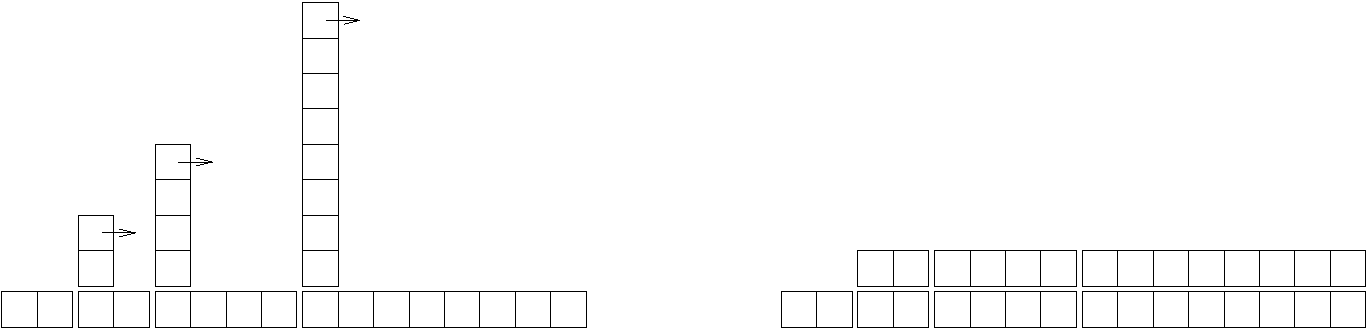
\includegraphics[width=5.5in]{figs/towers.pdf}}
\caption{哈希表元素添加成本图.\label{fig.hash}}
\end{figure}

再哈希所需要的额外消耗, 仿若一系列间距不断增加, 同时高度不断增长的高塔.
如果你推倒这些塔, 将调整空间大小的成本分摊到所有添加操作上, 
你可以从图中明显看到, $n$次添加操作的总成本为$2n-n$.

这个算法的一个重要特性是, 当我们调整哈希表大小时, 其耗时呈几何方式增长;
也就是说, 其大小乘以一个常数.
如果你增大其规模---每次增加固定数量---每次{\tt add}的平均耗时便是线性的.
\index{geometric resizing}

你可以从\url{http://thinkpython2.com/code/Map.py}下载我的哈希表的实现代码,
但请记住, 没有必要用它; 如果你想使用映射, 用Python的字典即可.

\section{术语表}

\begin{description}

\item[算法分析(analysis of algorithms):] 一种基于算法运行时间和/或所需空间, 比较算法优劣的方法. 
\index{analysis of algorithms}

\item[机器模型(machine model):] 一种计算机的简化表达方式, 用来描述算法.
\index{machine model}

\item[最糟糕情况(worst case):] 令给定算法运行最慢(或耗费空间最大)的输入.
\index{worst case}

\item[主导项(leading term):] 多项式中, 具有最高次幂的项.
\index{leading term}

\item[交点(crossover point):] 两种算法需要相同运行时间或空间的问题规模.
\index{crossover point}

\item[增长量级(order of growth):] 在算法分析中, 可以看作相同增长模式的函数集合.
比如, 所有耗时为线性变化的函数, 都属于同样的增长量级.
\index{order of growth}

\item[大O表示法(Big-Oh notation):] 用来表示增长量级的符号;
比如, $O(n)$表示耗时线性增长的函数集合. 
\index{Big-Oh notation}

\item[线性的(linear):] 一种运行时间和问题规模成比例变化的算法,
至少对大规模问题是如此.
\index{linear}

\item[二次方(quadratic):] 运行时间是$n^2$的算法, 其中$n$是问题规模的一个度量. 
\index{quadratic}

\item[检索(search):] 定位集合(列表或字典)中的元素或确认其不存在的过程.
\index{search}

\item[哈希表(hashtable):] 一种数据结构, 用来表示键-值对的集合, 同时
可以用常数时间进行检索.
\index{hashtable}

\end{description}


\printindex

\clearemptydoublepage
%\blankpage
%\blankpage
%\blankpage

\end{document}
